\documentclass[11pt,oneside]{ociamthesis}\usepackage[]{graphicx}\usepackage[]{color}
%% maxwidth is the original width if it is less than linewidth
%% otherwise use linewidth (to make sure the graphics do not exceed the margin)
\makeatletter
\def\maxwidth{ %
  \ifdim\Gin@nat@width>\linewidth
    \linewidth
  \else
    \Gin@nat@width
  \fi
}
\makeatother

\definecolor{fgcolor}{rgb}{0.345, 0.345, 0.345}
\newcommand{\hlnum}[1]{\textcolor[rgb]{0.686,0.059,0.569}{#1}}%
\newcommand{\hlstr}[1]{\textcolor[rgb]{0.192,0.494,0.8}{#1}}%
\newcommand{\hlcom}[1]{\textcolor[rgb]{0.678,0.584,0.686}{\textit{#1}}}%
\newcommand{\hlopt}[1]{\textcolor[rgb]{0,0,0}{#1}}%
\newcommand{\hlstd}[1]{\textcolor[rgb]{0.345,0.345,0.345}{#1}}%
\newcommand{\hlkwa}[1]{\textcolor[rgb]{0.161,0.373,0.58}{\textbf{#1}}}%
\newcommand{\hlkwb}[1]{\textcolor[rgb]{0.69,0.353,0.396}{#1}}%
\newcommand{\hlkwc}[1]{\textcolor[rgb]{0.333,0.667,0.333}{#1}}%
\newcommand{\hlkwd}[1]{\textcolor[rgb]{0.737,0.353,0.396}{\textbf{#1}}}%

\usepackage{framed}
\makeatletter
\newenvironment{kframe}{%
 \def\at@end@of@kframe{}%
 \ifinner\ifhmode%
  \def\at@end@of@kframe{\end{minipage}}%
  \begin{minipage}{\columnwidth}%
 \fi\fi%
 \def\FrameCommand##1{\hskip\@totalleftmargin \hskip-\fboxsep
 \colorbox{shadecolor}{##1}\hskip-\fboxsep
     % There is no \\@totalrightmargin, so:
     \hskip-\linewidth \hskip-\@totalleftmargin \hskip\columnwidth}%
 \MakeFramed {\advance\hsize-\width
   \@totalleftmargin\z@ \linewidth\hsize
   \@setminipage}}%
 {\par\unskip\endMakeFramed%
 \at@end@of@kframe}
\makeatother

\definecolor{shadecolor}{rgb}{.97, .97, .97}
\definecolor{messagecolor}{rgb}{0, 0, 0}
\definecolor{warningcolor}{rgb}{1, 0, 1}
\definecolor{errorcolor}{rgb}{1, 0, 0}
\newenvironment{knitrout}{}{} % an empty environment to be redefined in TeX

\usepackage{alltt}



% =================
% Macro definitions
% =================

\usepackage{amssymb}
\usepackage{hyperref}
\usepackage{graphicx}
\usepackage{booktabs}
\usepackage{tabularx}
\usepackage{amsmath}
\usepackage{algorithm}
\usepackage{algcompatible}
\usepackage{lscape}
\usepackage{rotating}
\usepackage{mathrsfs}
\usepackage{stmaryrd}
\usepackage{subcaption}
\usepackage{longtable}
\usepackage[noend]{algpseudocode}
\usepackage[font=normal,labelfont=bf]{caption}
\usepackage[superscript]{cite}
\usepackage[toc,page]{appendix}
%\usepackage[natbib=true,style=numeric,sorting=none]{biblatex}
\renewcommand{\citedash}{--}

\RequirePackage[osf,sc]{mathpazo}
\RequirePackage[scaled=0.90]{helvet}
\RequirePackage[scaled=0.85]{beramono}
\RequirePackage[T1]{fontenc}
\RequirePackage{textcomp}
\RequirePackage{titlesec,titletoc}

\titleformat{\chapter}[hang]{\itshape\huge}{\thechapter}{1em}{}[]
\titleformat{\section}[hang]{\normalfont\Large\itshape}{\thesection}{1em}{}[]
\titleformat{\subsection}[hang]{\normalfont\large\itshape}{\thesubsection}{1em}{}[]
\titleformat{\subsubsection}[hang]{\normalfont\normalsize\itshape}{\thesubsubsection}{1em}{}[]
\titleformat{\paragraph}[runin]{\normalfont\itshape}{\theparagraph}{1em}{}[]

%\titlespacing*{\chapter}{0pt}{50pt}{40pt}
%\titlespacing*{\section}{0pt}{3.5ex plus 1ex minus .2ex}{2.3ex plus .2ex}
%\titlespacing*{\subsection}{0pt}{3.25ex plus 1ex minus .2ex}{1.5ex plus.2ex}
%\titlespacing*{\subsubsection}{0pt}{3.0ex plus 1ex minus .2ex}{0.7ex plus.2ex}

\providecommand\newthought[1]{%
   \addvspace{1.0\baselineskip plus 0.5ex minus 0.2ex}%
   \noindent\textsc{#1} % small caps text out
}

\newcommand{\edge}{ %
  \mathrel{-}       % minus as a relation
  \joinrel\joinrel  % some backup
  \mathrel{-}       % minus as a relation
}

\graphicspath{{../motivation/figure/}{../background/figure/}{../detection/figure/}{../simulation/figure/}{../pf/figure/}{../chimp/figure/}{../discussion/figure/}}

% =============
% Configuration
% =============
\title{Hypothesis-free detection of genome-changing events in pedigree sequencing}
\author{Kiran V Garimella}
\college{Green Templeton College}
\degree{Doctor of Philosophy}
\degreedate{Hilary 2016}
\IfFileExists{upquote.sty}{\usepackage{upquote}}{}
\begin{document}

\baselineskip=18pt plus1pt  % this baselineskip gives sufficient line spacing for an examiner to easily markup the thesis with comments
\setcounter{secnumdepth}{3} % set the number of levels in each section heading
\setcounter{tocdepth}{3}    % set the number of levels in each chapter heading

% ========
% Preamble
% ========
\pagenumbering{gobble}
\maketitle                  % create a title page from the preamble info
\begin{dedication}
Dedication
\end{dedication}
        % include a dedication.tex file
\begin{acknowledgements}
Acknowledgements
\end{acknowledgements}
  % include an acknowledgements.tex file
\begin{abstract}

In high-diversity populations, a complete accounting of \textit{de novo} mutations can be difficult to obtain.  Most analyses involve alignment of genomic reads to a reference genome, but if the haplotypic background upon which a mutation occurs is absent, events can be easily missed (as reads have nowhere to align) and false-positives may abound (as the aligner forces the reads to align elsewhere).  In this thesis, I describe methods for \textit{de novo} mutation discovery and genotyping based on a so-called "pedigree graph" - a de Bruijn graph where all available sequencing data (trusted and untrusted data alike) is represented.  I constrain genotyping efforts to locations containing "novel kmers" - sequence present in the child but absent from the parents.  I then apply Dijkstra's shortest path algorithm to perform the genotyping, even in the presence of sequencing error.  In simulation, this approach provides a vastly more sensitive and specific set of \textit{de novo} variants than traditional methods.

In Chapter 1, I use part of a real dataset, progeny from the crossing of two \textit{Plasmodium falciparum} parasites, to demonstrate the pitfalls of the reference-based approach.  I also introduce de Bruijn graphs for genome assembly.

In Chapter 2, I present a review on mutational mechanisms that generate \textit{de novo} mutations, their rates, factors that influence their generation, and known events in various species.

Chapters 3 and 4 detail the software packages I have written for this work, the former including descriptions of the realistic variant read simulations, the latter detailing the graph genotyping algorithm.  Results from the application of the algorithm to the complete \textit{P. falciparum} dataset are presented in Chapter 5.

Finally, Chapter 6 discusses the work in a larger context and details various improvements that can be made in future work.

\end{abstract}
          % include the abstract
\pagenumbering{arabic}

\begin{romanpages}          % start roman page numbering
\tableofcontents            % generate and include a table of contents
\listoffigures              % generate and include a list of figures
\listoftables               % generate and include a list of tables
\listofalgorithms           % generate and include a list of algorithms
\end{romanpages}            % end roman page numbering

% ========
% Chapters
% ========
\chapter{Motivation}
\label{ch:motivation}

\section{Introduction}

\newthought{Spontaneously arising (\textit{de novo}) mutations} are rare genomic variants occurring within germ cells or the fertilized egg itself.  These variants are therefore absent from their parents' genomes, and in principle, straightforward to detect.  Modern experiments on second-generation sequencing platforms can now produce billions of short $75$ to $150$-bp reads during each instrument run.  These experiments are relatively inexpensive, making it feasible to generate moderate to high coverage data for members of a pedigree in mere hours or days.  Aligned to a reference, a canonical representation of a genome for a single member of the species, consistent differences at a single genomic position within reads that span the locus reveal genomic variants.  Sufficiently high coverage helps statistical software to distinguish sequencing error from true variation, and searches for alleles present in a child but absent in its parents can yield a candidate set of \textit{de novo} mutations (DNMs).

This protocol, widely adopted and applied in a variety of datasets, makes a tacit assumption: the reference genome and a new sample's genome should be nearly identical in sequence.  This assumption is necessary and is typically reasonable: when working with samples having a low heterozygosity, most sites in the genomes of two or more samples should be identical, and occasional differences are small and easily handled by read-to-reference alignment methods that are capable of tolerating a small amount of heterology.

However, there are plenty of loci within genomes that do not meet this assumption.  Different strains of the uropathogenic bacterium \textit{Escherichia coli} are reported to have strain-specific genomic islands containing virulence factors that are entirely absent from the laboratory strain $MG1655$ used as the basis for the reference sequence\cite{Fukiya:2004cn}.  In assembled samples from the diploid coccolithophore \textit{Emiliania huxleyi}, $8$ to $40$ Mbp of the approximately $142$ Mbp genome was shown to be isolate-specific; $25\%$ of genes in the reference strain, CCMP1516, were not found in the other $13$ examined isolates\cite{Read:2013bf}.  The human major histocompatibility complex (MHC), a $163$ Mbp region of chromosome $6$ that encodes genes critical to innate and adaptive immunity\cite{Mungall:2003br,Shiina:2009iy}, exhibits tremendous population diversity\cite{GonzalezGalarza:2014cd} and can generally not be recovered by simple alignment to the reference, but \textit{can} be reconstructed with high accuracy by aligning data to an augmented version of the reference with alternative loci included\cite{Dilthey:2015dq}.

When a haplotype represented in a canonical reference sequence differs substantially from a sample under study, sequenced reads spanning gross differences may behave in two different ways: either they fail to align anywhere in the reference, or they align incorrectly.  In the former case, interesting inter-sample variation in those regions is lost.  In the latter case, the incorrect alignments may generate false-positive variant calls.  This constitutes a reference bias: samples similar to the reference align properly and their genomic content can be analyzed easily.  Those sufficiently dissimilar cannot.

Reference bias may thwart complete discovery of \textit{de novo} mutations, a class of mutations particularly important in the study of pathogens.  For example, a single serine to asparagine amino acid substitution (S31N) in influenza A alters the properties of the $M_2$ ion channel\cite{Wang:1993uc}, interferes with the action of the adamantane class of antiviral drugs, and has reached fixation in the population\cite{Nelson:2009en}.  In \textit{Mycobacterium tuberculosis}, a four-year \textit{in vitro} drug challenge experiment on nine drug-susceptible isolates from a single patient demonstrated the strain could acquire resistance to nearly all first-line and most second-line drugs through just $12$ single nucleotide polymorphisms (SNPs)\cite{Eldholm:2014ei}.  \textit{Staphylococcus aureus} is the most common cause of post-operative infection worldwide and is increasingly unresponsive to $\beta$-lactam treatment and drugs in the penicillin group (methicillin, dicloxacillin, nafcillin, oxacillin, etc.).  Sequencing of methicillin-susceptible (MSSA) in the penicillin group and resistant (MRSA)\footnote{The term "methicillin resistant" is used in the literature, though it is commonly taken to mean all drugs, including more stable variants of methicillin used in modern clinical practice.} strains reveals the acquisition of resistance genes via mobile genetic elements and horizontally transferred genomic islands (e.g. the SCC\textit{mec} cassette chromosome upon which the methicillin and other $\beta$-lactam antibiotic resistance gene, \textit{mecA}, resides)\cite{Holden:2004kd}.

\section{\textit{De novo} mutations (DNMs) in \textit{Plasmodium falciparum}}

\begin{table}[]
\centering
\caption{Phenotypes of \textit{P. falciparum} isolates used for genetic crosses.}
\label{tb:pf_phenotypes}
\begin{tabular}{@{}rcccccc@{}}
\toprule
                                 & 3D7 & HB3 & DD2 & 7G8 & GB4 & 803 \\
\midrule
pyrimethamine sensitivity        & -   & +   &     &     &     &     \\
chloroquine sensitivity          &     & +   & -   &     &     &     \\
infects mosquitoes easily        &     & +   & -   &     &     &     \\
infects \textit{Aotus nancymaae} &     &     &     & -   & +   & -   \\
artemisinin sensitivity          &     &     &     &     & +   & -   \\
\bottomrule
\end{tabular}
\end{table}

To see how reference bias may affect DNM discovery, let us consider a second-generation sequencing dataset on experimental crosses of \textit{Plasmodium falciparum} parasites, the etiological agent for the most deadly form of malaria.  These crosses have enabled the discovery of a number of inherited and \textit{de novo} virulence factors.  The contrasting phenotypes for various strains of \textit{P. falciparum} are listed in Table \ref{tb:pf_phenotypes}.  For inherited factors, crossing of the pyrimethamine-resistant 3D7 and sensitive HB3 strains~\cite{Walliker:1987cv} revealed a non-synonymous point mutation in the \textit{dhfr-ts}\footnote{dihydrofolate reductase-thymidylate synthase} gene, inhibiting binding of (and thus conferring resistance to) the drug~\cite{Peterson:1988wt}.  Analysis of the HB3 x DD2 cross\cite{Wellems:1990eg}, the latter of which is resistant to chloroquine, localized the determinant to a previously undetected gene on chromosome $7$, labelled \textit{pfcrt}\footnote{\textit{P. falciparum} chloroquine resistance transporter}, a member of a new family of transporters.  Additional investigation into differences in mosquito infection efficacy revealed down-regulation of the \textit{pfmdv-1}\footnote{\textit{P. falciparum} male gametocyte development gene 1} gene~\cite{Vaidya:1995up,Furuya:2005jn}, disruption of which results in marked reduction of mature and functional male gametocytes.

For uninherited factors, cytoadherence and antigenic properties of parasites facilitate evasion from host immune attack, and can differ substantially from the properties of their progenitors.  In 2000, Freitas-Junior \textit{et al.} showed that some 3D7 x HB3, HB3 x DD2, and HB3 x HB3 progeny harbored non-parental forms of subtelomeric \textit{var} genes, key members of an antigenic gene family\cite{FreitasJunior:2000cp}.  These altered forms were likely generated during mitosis by non-allelic homologous recombination\footnote{sometimes referred to as "ectopic" (aberrant) recombination in the literature} (NAHR) of telomeres from two different chromosomes\cite{Duffy:2009cc}.  The resulting genes are novel, functional, and never before observed by the host immune system.

These DNMs are critical tools for malaria to evade drug and immune pressure.  NAHR can further diversify a pathogen's antigenic repertoire, enabling continued evasion of immunological actors.  Duplications of a transporter gene may enable faster drug clearance in a parasite, thus conferring resistance.  Spontaneous point mutations may alter the binding site of a drug to a receptor, thus conferring immunity. 

\subsection{A reference-based approach for DNM discovery and genotyping}

With the advent of sequencing technologies, it is now straightforward to discover many DNMs.  Long reads (\textasciitilde $500$ bp) from the first-generation sequencing technology, Sanger sequencing, can be stitched together \textit{in silico} by considering the overlaps of sequences generated from many copies of the genome\cite{Myers:1995vma}.  This has enabled the reconstructions of full-length genomes and subsequent gene annotations for a single representative (or "reference") individual in a population.  Second-generation sequencing is leveraging economies of scale to reduce sequencing costs by several orders of magnitude\cite{Mardis:2011cr}.  The reads it produces are shorter (\textasciitilde $100$ bp) and more error-prone, but billions of them can be produced quickly.  Like the long reads, the short read data can also be assembled into a new genome, albeit with more errors and gaps, owing to the difficulty of overcoming large repetitive regions with short genomic fragments\cite{Schatz:2010if}.  Alternatively, assuming the sequence for the reference genome and a new individual are highly similar, it is far more common (and computationally more efficient) to align the reads to the reference\cite{Flicek:2009dl}.  String matching algorithms that allow mismatches, insertion, and deletions to appear in the alignments allow millions of sequenced reads to be placed on the reference genome quickly.  Separate tools can then examine the alignments, looking for the presence of non-reference alleles, and using statistical approaches to call and genotype variants with high accuracy\cite{Nielsen:2011kz}.

Variant calling software has been successfully applied to many sequencing datasets for the discovery of DNMs.  These variant callsets have provided insight into the development of drug resistance\cite{Woodford:2007it}, the genetic architecture of some common diseases\cite{Neale:2012ki}, and mutational rates in humans and chimpanzees with a strong paternal age effect\cite{Conrad:2011eh,Venn:2014ep,Kloosterman:2015cn,Francioli:2015kj}.  Many groups have released sophisticated software packages to facilitate these analyses and detailed instructions on their use\cite{DePristo:2011fo,Rimmer:2014ho}.

\subsection{A reference-free approach for assessing DNM sensitivity}

Specificity and sensitivity are crucial metrics to consider for any variant callset.  There are many approaches to establishing the specificity of a DNM callset.  For select variants (typically on the order of \textasciitilde $100$ variants from a callset), Sanger sequencing, Sequenom assays, and even targeted third-generation sequencing (i.e. PacBio sequencing, which can generate reads up to \textasciitilde $50,000$ bp as of this writing) have been used successfully to validate mutations.  Establishing sensitivity is much more difficult.  In theory, one would need complete and error-free reference genomes for both parents and each child in which the mutation calls are made.  Except for the smallest genomes, such an approach is prohibitively expensive.

Instead, it may be possible to establish the sensitivity of the reference-based protocol by considering how DNMs alter the genome of a sample with respect to its progenitors.  Consider a site where a DNM - say, a single SNP - has occurred, as depicted in Figure \ref{fig:kmer_venn}.  Although a single base of the genome has been altered, when the genome is divided into fixed-length words of length $k$, or "kmers", we find $k$ kmers that are present in the child but absent in the parents.  In this manner, DNMs can be considered generators of "novel" kmers - kmers present in the child but absent in the parents.  These kmers can be used as a signal to indicate the presence of a \textit{de novo} variant.  By choosing $k$ to be reasonably large so as to avoid analyzing short sequences that pervade the genome (half to two-thirds the length of a read will suffice), we can simply count continuous stretches of novel kmers as a proxy for the number of DNMs.

\begin{figure}[h!]
  \centering
    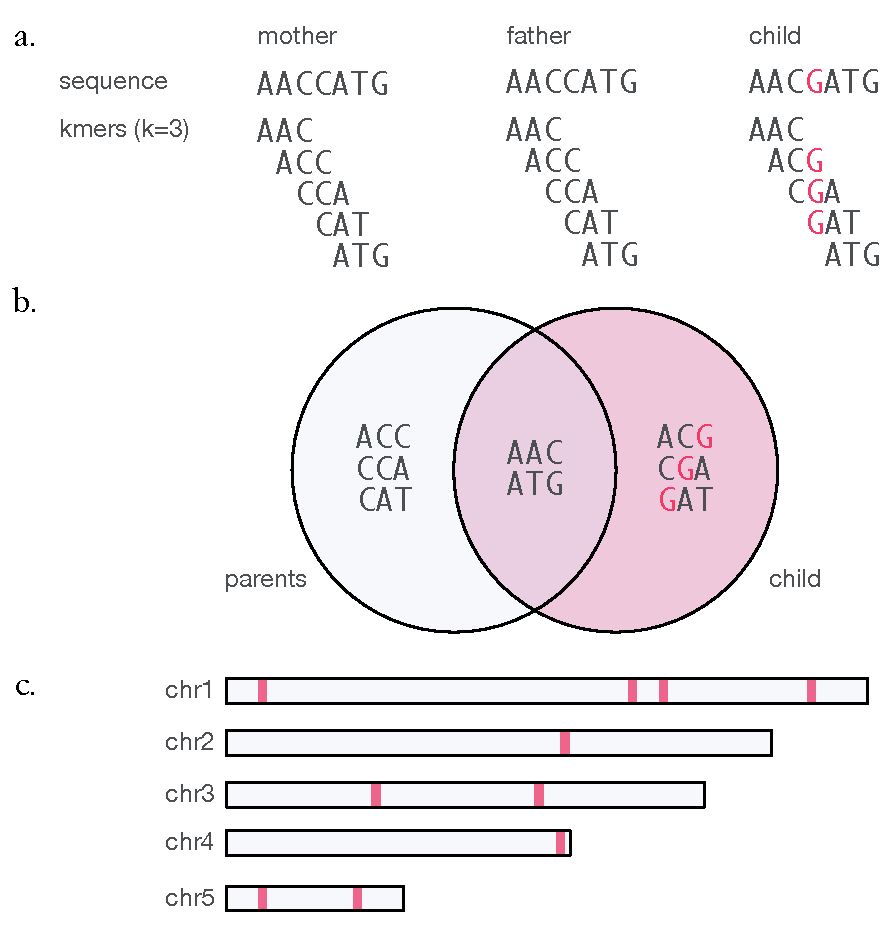
\includegraphics[width=0.8\textwidth]{kmer_venn}
  \caption{a. Parental and child sequences at the site of a \textit{de novo} mutation, and the kmers generated at $k=3$.  b. The resulting Venn diagram of kmers found exclusively in the parents, the child, or common to both.  c. Novel kmers found around the genome indicate the presence of a \textit{de novo} mutation.}
  \label{fig:kmer_venn}
\end{figure}

This approach gives us a powerful, reference-free mechanism to verify the results of the reference-based analysis.  Sequencing of the whole genome is independent of any reference sequence that may already exist for the sample, and given sufficient coverage (Table \ref{tb:lw_cov} shows the requirements, assuming $76$ bp reads and a $23$ megabase genome), the raw data from a sequencing experiment should contain the full set of DNM-generated novel kmers, regardless of any mapping issues\cite{Lander:1988bp}.  Taking the reads that map, calling \textit{de novo} variants, and extracting the novel kmers from the immediate vicinity should theoretically reproduce that set.  Comparing the expected (reference-free) set to the observed (reference-based) kmer set should thus provide the sought sensitivity measure.

\begin{table}[]
\centering
\caption{Theoretical percentage of the genome recovered at a target depth of coverage.}
\label{tb:lw_cov}

\begin{tabular}{llll}
\toprule
coverage & reads & nucleotides covered & genome (\%)\\
\midrule
1 & 302631 & 2.3e+07 & 63.21\\
2 & 605263 & 4.6e+07 & 86.47\\
3 & 907894 & 6.9e+07 & 95.02\\
4 & 1210526 & 9.2e+07 & 98.17\\
5 & 1513157 & 1.15e+08 & 99.33\\
6 & 1815789 & 1.38e+08 & 99.75\\
7 & 2118421 & 1.61e+08 & 99.91\\
8 & 2421052 & 1.84e+08 & 99.97\\
9 & 2723684 & 2.07e+08 & 99.99\\
10 & 3026315 & 2.3e+08 & 100.00\\
11 & 3328947 & 2.53e+08 & 100.00\\
12 & 3631578 & 2.76e+08 & 100.00\\
13 & 3934210 & 2.99e+08 & 100.00\\
14 & 4236842 & 3.22e+08 & 100.00\\
15 & 4539473 & 3.45e+08 & 100.00\\
\bottomrule
\end{tabular}


\end{table}

\section{DNM sensitivity of the reference-based approach}

We now test these ideas on part of a real dataset that will be used throughout this dissertation: experimental crosses between malaria parasites (\textit{Plasmodium falciparum}).  For simplicity, we shall focus on $17$ samples from the 3D7xHB3 experimental cross, sequenced to an average fold-coverage of $105 \pm 34$, using $76$ bp reads.

%, and a two-generation pedigree of human's closest extant ancestor (and susceptible to \textit{falciparum} malaria), chimpanzees (\textit{Pan troglodytes})\footnote{Note that, while chimpanzees are used as an \textit{in vivo} model for the malaria parasite's liver stage in the production of the crosses, these two datasets are not related to one another.}.

%The datasets that we'll be referring to in this work are summarized in Table \ref{tb:cross_info}.  For simplicity, we shall focus on the samples from the 3D7xHB3 cross.
%
%\begin{table}[]
%\centering
%\caption{The \textit{P. falciparum} datasets that will be referred to throughout this work.}
%\label{tb:cross_info}
%\begin{tabular}{@{}rcccc@{}}
%\toprule
%                  & 3D7xHB3      & HB3xDD2      & 7G8xGB4      & 803xGB4      \\
%\midrule
%progeny           & $17$         & $30$         & $38$         & $29$         \\
%read length       & $76$         & $76$         & $76$         & $100$        \\
%fragment size     & $300 \pm 30$ & $248 \pm 46$ & $294 \pm 17$ & $224 \pm 8$  \\
%coverage          & $105 \pm 34$ & $102 \pm 48$ & $105 \pm 30$ & $176 \pm 54$ \\
%\bottomrule
%\end{tabular}
%\end{table}

\subsection{Data processing}
We first generated the list of expected novel kmers by processing the raw sequencing data for each sample with the \textit{de novo} assembly software, Cortex\cite{Iqbal:2012fx} at $k=47$, standard settings for other parameters, and no error cleaning.  We produced the initial list of putative novel kmers by selecting kmers present in a child but absent in both parents.  We further filtered this list in a number of ways.  First, we imposed lower and upper kmer coverage thresholds, automatically determined by a custom algorithm designed to find a local minimum on the LOESS regression of the coverage distribution, as shown in Figure \ref{fig:kmer_cov_dist}.  Additionally, we removed kmers originating from possible contaminants, as determined by performing a BLAST search on the confident list, removing all non-\textit{Plasmodium} hits, and any putatively novel kmers connected to them in the graph.  More details on these steps are presented in Chapter \ref{ch:realdata}.  These steps ensure that the list of novel kmers is very restrictive.

\begin{figure}[h!]
  \centering
    \includegraphics[width=0.8\textwidth]{{{PG0063-C.ERR019060.kmerCovThreshold}}}
  \caption{Kmer coverage distribution for a single 3D7xHB3 progeny, PG0063-C.  Red line indicates non-parametric LOESS fit upon which the local minimum is detected.}
  \label{fig:kmer_cov_dist}
\end{figure}

We aligned each sample's reads to the PlasmoDB 9.0 release of the \textit{Plasmodium falciparum} genome\cite{Gardner:2002p1564,Aurrecoechea:2009hh} using BWA-MEM\cite{Li:2013wn}.  We followed data processing guidelines as specified in the Genome Analysis Toolkit (GATK) best-practices documentation\cite{DePristo:2011fo,McKenna:2010p535}, flagging duplicate reads so that they are ignored downstream, and recalibrating base quality scores using the MalariaGen data release on the crosses as a truth set\cite{Miles:2015in}.  As recent guidance by the authors indicates the GATK's variant calling software has internalized the local indel realignment functionality, we opted to forego running this step separately.  We called variants across all $18$ samples (parents and progeny) simultaneously using the GATK's HaplotypeCaller with standard settings and a ploidy of $1$.

\begin{algorithm}
\caption{Given a small set of variants, generate all possible subsets of variants}
\label{alg:all_subsets}
\begin{algorithmic}[1]
\Function{generateAllPossibleSubsets}{variants}
    \State $\textit{los} \gets []$

    \For{$i \gets 0 \textrm{ to } length(variants)$}
        \State $\textit{lo} \gets []$

        \For{$j \gets 0 \textrm{ to } length(variants)$}
            \If{$i \neq j$}
                \State $\textit{lo.add(variants[j])}$
            \EndIf
        \EndFor

        \If{$\textit{lo.size()} \ge 0$}
            \State $\textit{los.add(lo)}$
        \EndIf

        \If{$\textit{lo.size()} \ge 1$}
            \State $\textit{generateAllPossibleSubsets(lo)}$
        \EndIf
    \EndFor

    \State $\textit{return los}$
\EndFunction
\end{algorithmic}
\end{algorithm}

A complete and perfect variant callset details the alterations that must be performed on the reference sequence in order to generate the genome of the sequenced sample.  Unfortunately, it is typically not possible to obtain a perfectly sensitive and specific callset.  False positives and false negatives proximal to true positives may interfere with our ability to generate the true underlying haplotype sequence.  To bypass this problem, we did not filter the variant callset.  Instead, we combinatorically generated all possible subsets of variants found within $100$ bp of each other using a recursive strategy to leave single elements out of a given set of kmers, presented in Algorithm \ref{alg:all_subsets}.  This will certainly generate vastly more kmers than truly exist in the sample's genome.  However, as we are only interested in verifying that the variant-induced kmers are present in our novel kmer set, this approach has the benefit of providing maximum sensitivity.

\subsection{Results}

\begin{figure}[h!]
  \centering
    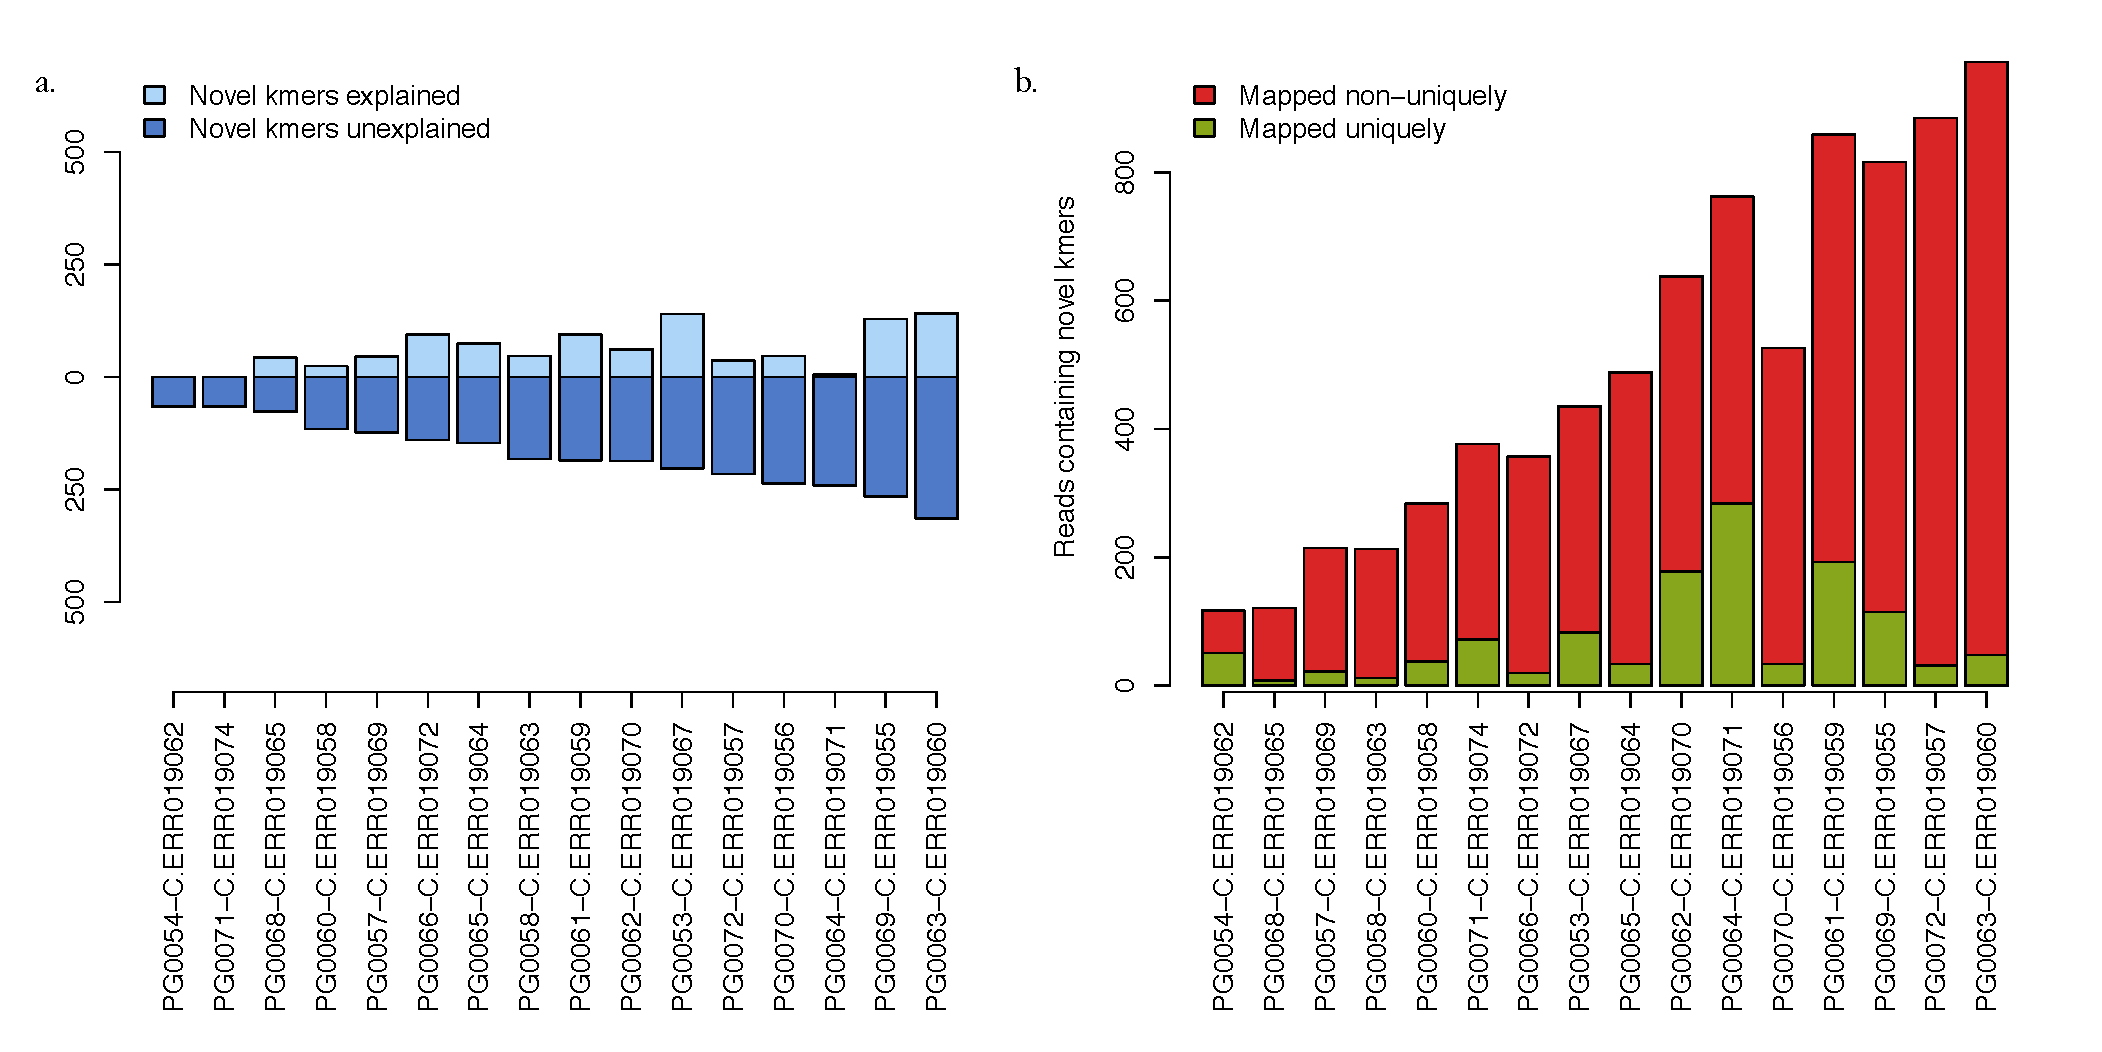
\includegraphics[width=\textwidth]{reffailure}
  \caption{a. Novel kmers observed in the reference-based analysis vs novel kmers expected from the reference-free analysis.  b. Reads that map once to the reference genome versus mapping multiple times, conditioned on the read containing a novel kmer.}
  \label{fig:reffailure}
\end{figure}

%\begin{figure}[h!]
%  \centering
%    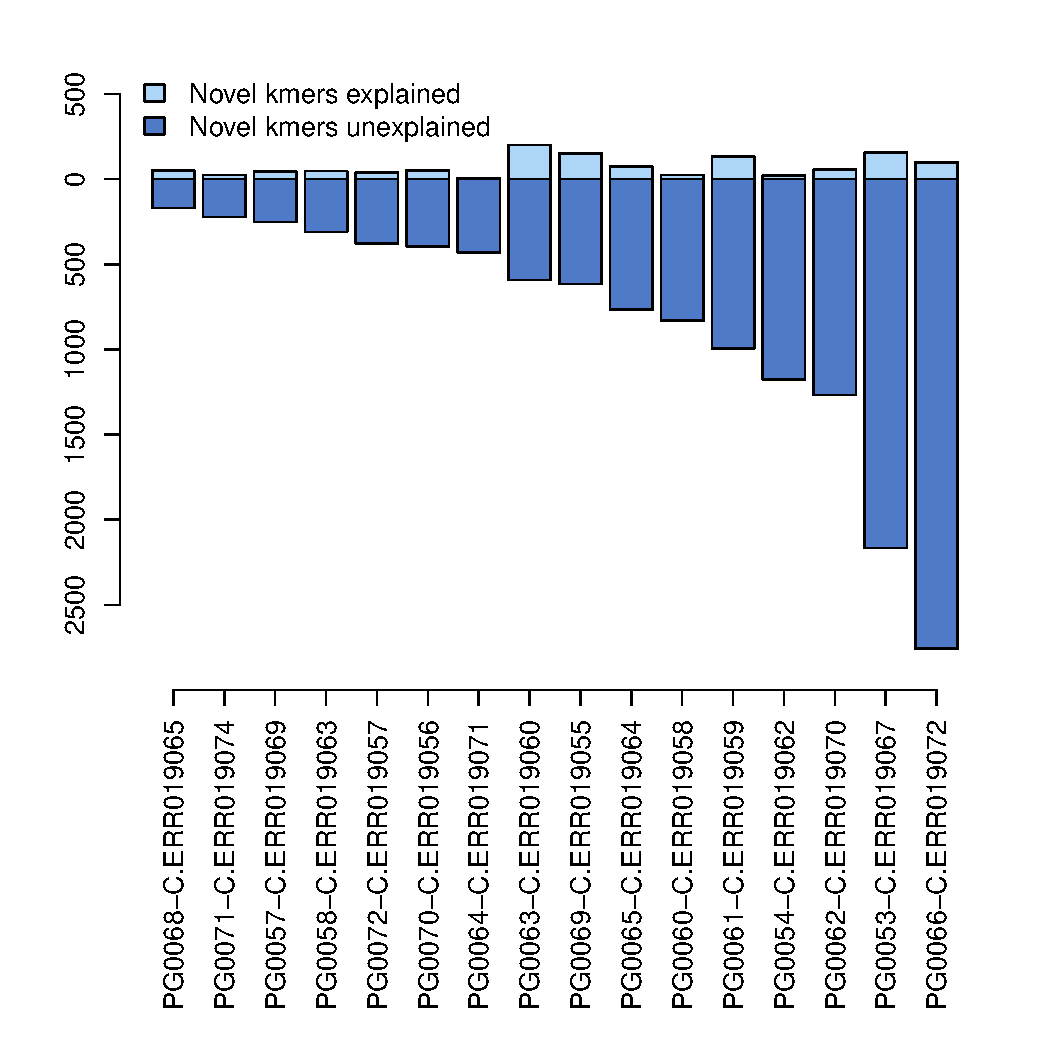
\includegraphics[width=0.8\textwidth]{loadTables-1}
%  \caption{Novel kmers observed in the reference-based analysis vs novel kmers expected from the reference-free analysis.}
%  \label{fig:obs_vs_exp_kmers}
%\end{figure}

Figure \ref{fig:reffailure}a shows the results of our reference-based vs reference-free analysis.  Per sample, our restrictive reference-free analysis has generated hundreds of novel kmers to explain.  However, the reference-based analysis recapitulates only a fraction of these - about $36\%$ on average.

Attempting to explain where these missing kmers have gone, we searched the reads for every novel kmer.  On average, more than $80\%$ of reads containing these kmers were found to map to multiple homes in the genome (summarized per sample in Figure \ref{fig:reffailure}b).

%\begin{figure}[h!]
%  \centering
%    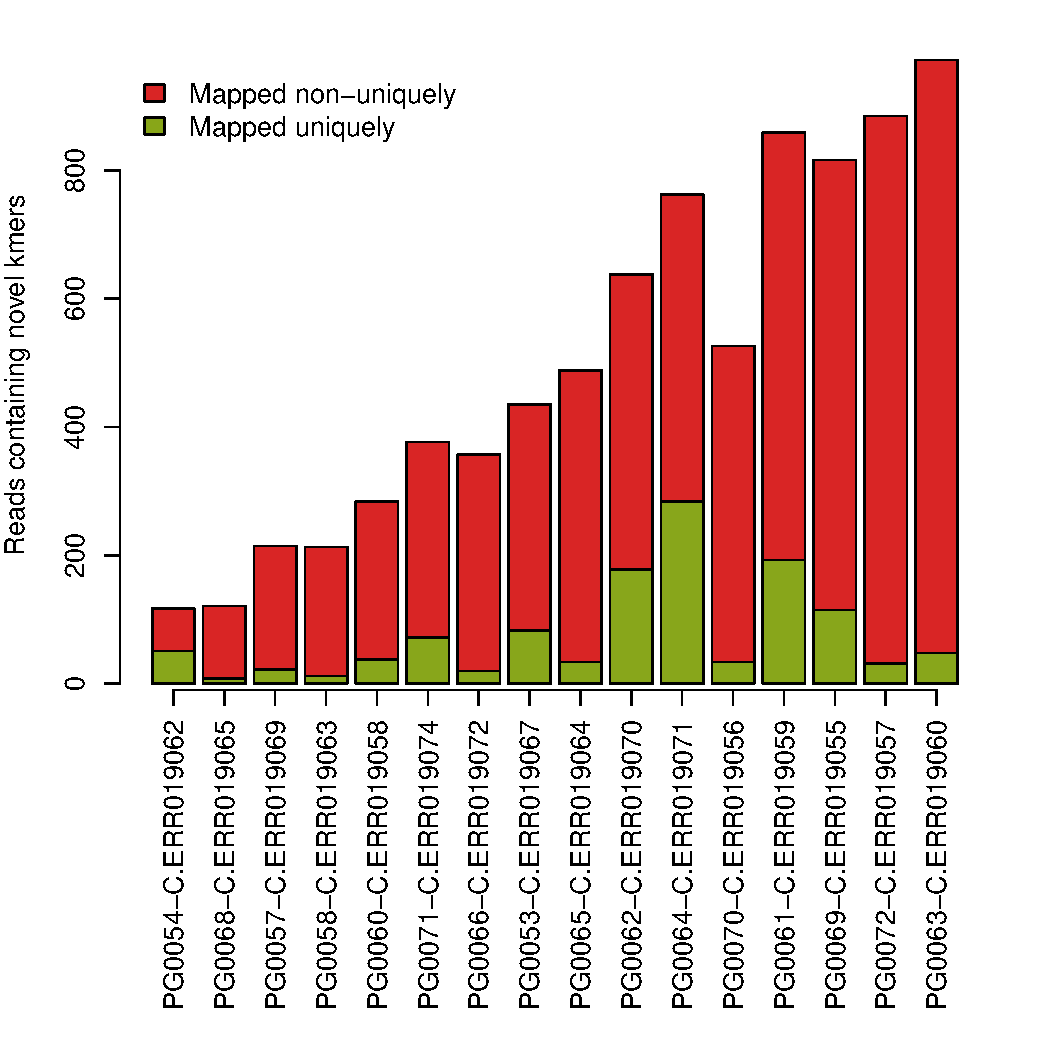
\includegraphics[width=0.8\textwidth]{mapping-1}
%  \caption{Reads that map once to the reference genome versus mapping multiple times, conditioned on the read containing a novel kmer.}
%  \label{fig:mapping}
%\end{figure}

\section{Discussion}
\subsection{Failure of the mapping approach}

The preponderance of reads containing novel kmers fail to map uniquely to the reference genome, explaining why we should find such a massive discrepancy between the novel kmers we expect versus explain - reference-based calling approaches cannot call variants on unplaced reads.  That there should be so many reads that fail to map is perhaps not surprising, given the divergent nature of the reference genome to other samples.  Figure \ref{fig:ref_venn_HB3} shows the overlap between kmer sets between the 3D7 and HB3 genomes.  More than $20\%$ of the total set of kmers between these two samples is unique to each sample.

\begin{figure}[h!]
  \centering
    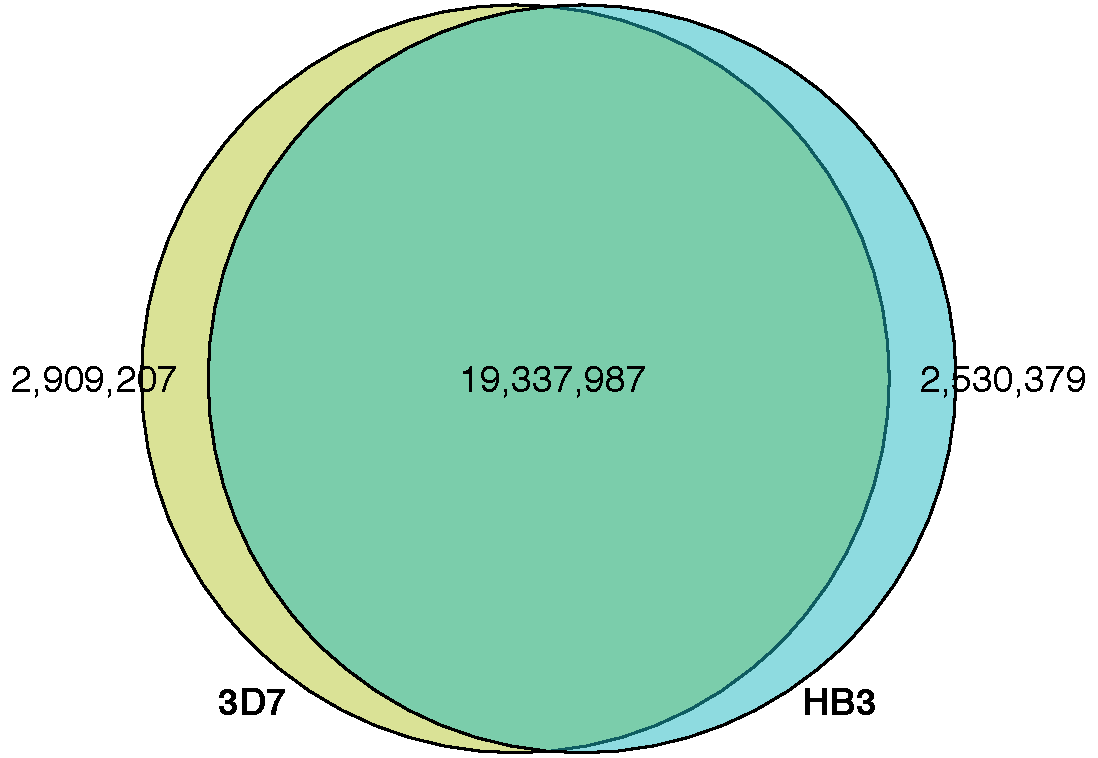
\includegraphics[width=0.8\textwidth]{ref_venn_HB3}
  \caption{Venn diagram of kmers present in the 3D7 and HB3 genomes at $k=47$.  Both forward and reverse-compliment kmers are considered the same.}
  \label{fig:ref_venn_HB3}
\end{figure}

These unique kmers are not simply repetitive, intergenic, or otherwise uninteresting.  They often reflect interesting biology.  Figure \ref{fig:kmer_recovery} shows one example: three \textit{var} genes from 3D7's $60$-member antigenic repertoire.  These genes do not overlap with the HB3 repertoire.  One of the 3D7xHB3 progeny, has inherited one of the 3D7 \textit{var} genes in full, but curiously exhibits mosaic recovery of two others.  This is known to be an NAHR event between the telomeres of chromosomes $1$ and $2$, likely to have occurred during mitosis, preserving the domain architecture and yielding a functional product\cite{Claessens:2014fo}.

%\begin{sidewaysfigure}[h!]
\begin{landscape}
\begin{figure}
  \centering
    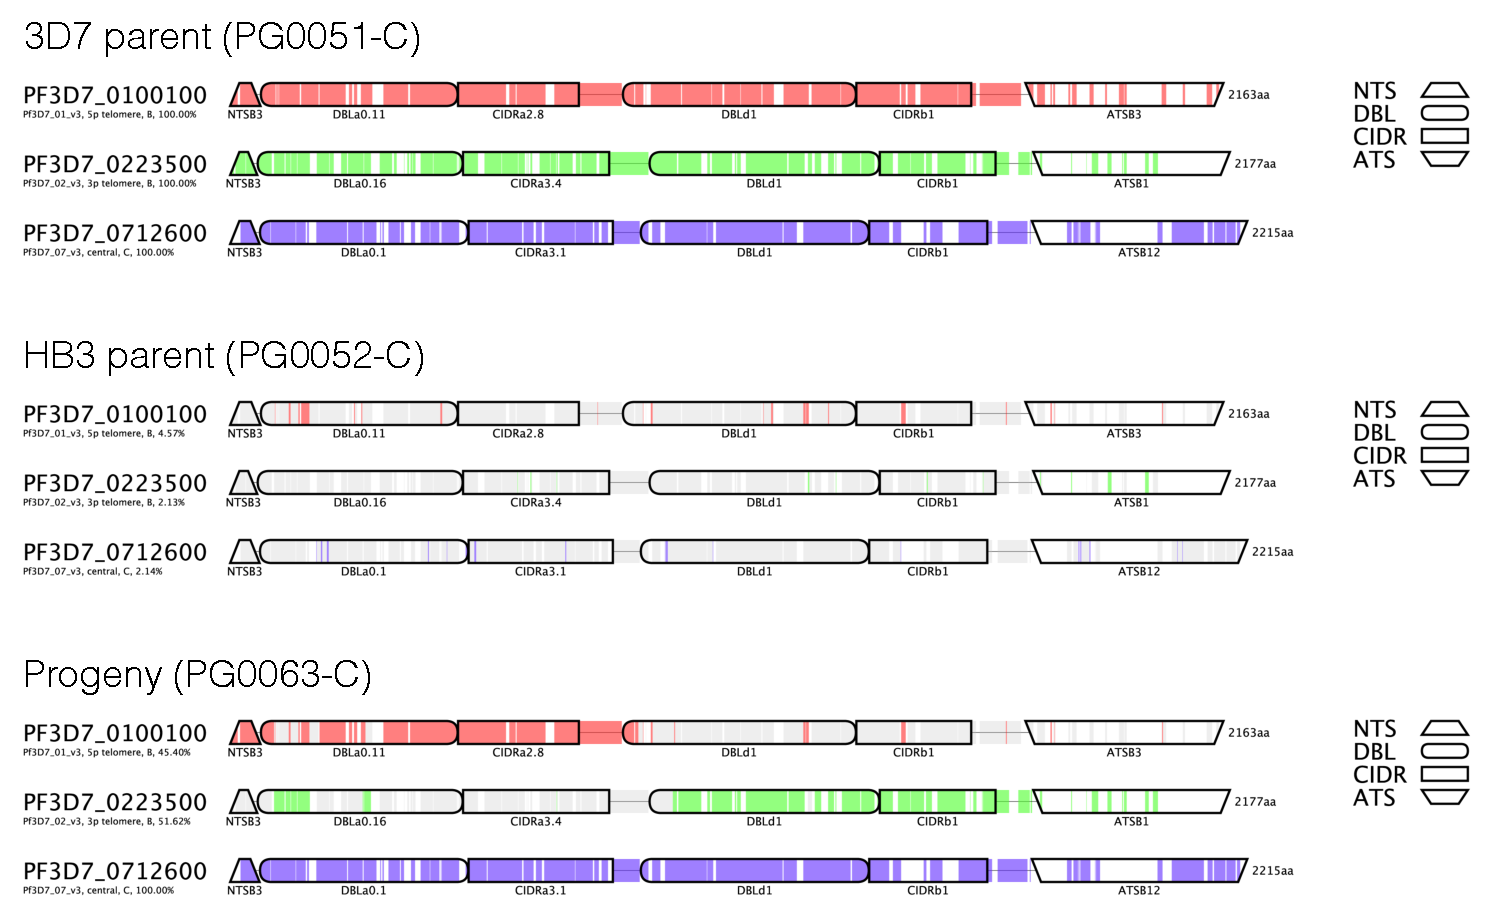
\includegraphics[width=1.45\textwidth]{kmer_recovery}
  \caption{Presence and absence of unique kmers in three 3D7 \textit{var} genes.  Each vertical line represents a kmer.  Colored kmers represent those unique 3D7 kmers that are recovered in the sample.  Grey indicates no recovery.  White indicates the kmer at that position was not unique in the 3D7 genome.  Only the coding regions of the respective genes are shown, with domain annotations obtained from the VarDom server\cite{Rask:2010fia}.}
  \label{fig:kmer_recovery}
\end{figure}
\end{landscape}
%\end{sidewaysfigure}

Alignment of short reads to a single reference and subsequent application of variant callers is a poor strategy for \textit{de novo} variant discovery in \textit{P. falciparum} (and likely higher-order species as well) for a number of reasons:

\begin{enumerate}
\item \textbf{Absent or divergent loci in genome} \hfill \\ The underlying assumption that two genomes from the same species should be very similar is inappropriate for highly diverse populations (e.g. pathogens) or hypervariable regions (e.g. immune loci in mammals).  If a haplotype present in the sample is too dissimilar to the reference, or perhaps even completely absent, read aligners may return incorrect results.  Reads may align to the wrong location, the resultant mismatches mistaken for real mutations.  Alternatively, they may fail to align at all, thus obscuring evidence of real variation.

\item \textbf{Incomplete or errorful reference sequences} \hfill \\ Reference sequences are often incomplete and/or contain errors due to technical artifacts.  Chaisson \textit{et al.} provide an excellent review on the various errors that may arise\cite{Chaisson:2015dg}.  Regions of the genome may fail to amplify during library preparation, leading to coverage dropout and subsequent gaps in the assembly.  Insufficiently long reads used in the reference genome construction may lead to the misestimation of lengths of repetitive regions, causing repeats to have a collapsed representation relative to the true genome.  Segmental duplications, gene families, or other loci with high sequence identity may generate ambiguous read overlaps that cannot be resolved without very long reads.

\item \textbf{Difficult to include prior information about variation in a species} \hfill \\ Read aligners must make a decision as to how many apparent mismatches to permit with respect to the reference sequence.  However, these software packages typically operate per-read, without information on prior population variation throughout the genome.  

\item \textbf{Inability to include improved or project-specific data} \hfill \\ Improvements in sequencing technology, or new platforms altogether, can yield supplementary datasets that adds missing information to a genome or repairs a misrepresented locus.  There is no natural framework for incorporating these additional datasets to the alignment framework.
\end{enumerate}

\begin{figure}[h!]
  \centering
    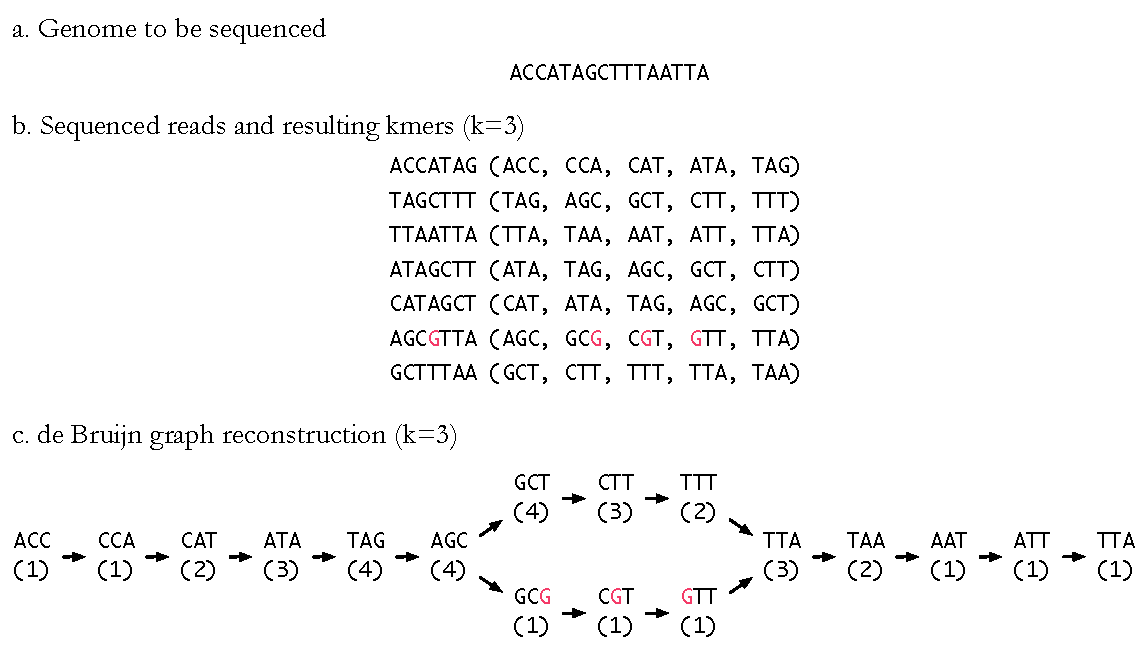
\includegraphics[width=\textwidth]{debruijn}
  \caption{The process of generating a de Bruijn graph representation of sequence data.  a. The underlying genome. b. Reads sequenced from the genome (including one read with a sequencing error).  Reverse-complement reads are not shown for clarity.  c. The $k=3$ de Bruijn graph reconstruction, including kmer coverage annotations.}
  \label{fig:debruijn}
\end{figure}

\subsection{\textit{De novo} assembly as an alternative approach}

Consider Table \ref{tb:lw_cov} again, which demonstrates that we can expect to recover the full genome at as little as $10$-fold coverage.  For small genomes (\textit{P. falciparum} is approximately $23$ megabases in length), modern sequencing experiments can routinely return excess of $100$-fold coverage.  It is therefore clear that deeply-sequenced samples will have reads representing the entirety of the genome despite our inability to align all of them to the genome.  Rather than relying on mapping to an imperfect and incomplete reference, we can attempt to assemble the genome \textit{de novo} - from the sequenced data itself, ignoring the availability of a reference sequence.

The problem of performing \textit{de novo} assembly essentially reduces to computing read-to-read alignments, rather than read-to-reference alignments.  As each read represents recovery of some small region of the genome, the supersequence of overlapping reads (the aligned nucleotides flanked by the non-overlapping sequences from each read) represent some larger linear stretch of the genome.  Brute-force computation of all possible pairwise alignments is $\mathcal{O}(N^2)$ in the number of reads, which is impractical for second-generation sequencing datasets with tens or hundreds of millions of reads.  Fortunately, there are many ways to compute and represent these overlaps efficiently.  We shall focus on one $\mathcal{O}(N)$ method in this work: assembly via construction of a de Bruijn graph.

Formal definitions can be found in Chapter \ref{ch:methods}.  Informally, a graph is simply a data structure representing a collection of objects (termed "vertices" or "nodes") and connections ("edges" or "links").  In a de Bruijn graph, each vertex is a unique element.  Applied to sequencing, a de Bruijn graph encodes linear stretches of sequence, while each edge represents an overlap with the connected vertices.  Commonly, each read is decomposed into fixed-length words of an arbitrary length $k$, or "kmers".  As each kmer is sequentially extracted from a read and added to the graph as vertices, edges between adjacent kmers in the read are stored as well.  Overlapping reads will share kmers, and since each kmer can only appear once in the graph, adding kmers and edges from the overlapping read effectively records the alignment without needing to literally compute all possibilities.  Figure \ref{fig:debruijn} depicts a simple $16$ bp genome, sequenced with $7$ bp reads, and the resulting de Bruijn graph constructed at a kmer size of $3$.

Construction of this data structure is challenging.  First, errors in second-generation sequencing data are very common, and therefore the graph produced from raw sequencing data will contain many branches that are not in the actual genome (examine Figure \ref{fig:debruijn} again, observing the highlighted base - a sequencing error - and the resultant perturbation to the otherwise linear graph).  These can be mitigated (but perhaps not completely solved) by error-cleaning algorithms that remove low coverage kmers, as presumably in high coverage data, random errors are rare and can be detected and discarded.  Second, long repetitive stretches of the genome that feature the same kmers multiple times will be collapsed into a single copy, as de Bruijn graphs only store each kmer once.  Finally, homology in the genome can cause two separate regions of the genome to appear adjacent to one another in the graph.  This may result in a vertices with multiple outgoing edges, causing unresolvable ambiguity when traversing the graph.

Nevertheless, such an approach should resolve many of the deficiencies of an alignment-based approach.  Absent or divergent loci should be recovered.  The uncleaned graph should be complete (barring any regions of the genome that suffer from an amplification bias that prevents them from being sequenced).  Prior information about variation in the species (or in this case, just the parents) are included by assembling the parents and comparing to them directly, rather than indirectly via the reference.  Finally, additional information can be added at graph construction time or by adding a separate color to the graph encoding the supplementary data.

\section{Overview of this work}

In this dissertation, we present a novel multi-color graph-based approach to \textit{de novo} mutation detection and allele identification.  We show how knowledge of the pedigree enables us to identify so-called novel kmers - kmers present in children and absent from parents - that serve as an exceedingly strong signal as to the presence of \textit{de novo} variation.  We use these kmers to analyze subgraphs in the genome likely to represent DNMs and navigate color-specific paths and trails to determine the precise allele.  We also demonstrate how the novel kmers act as "sign posts" during graph traversal, indicating that a traversal is following a fruitful path.  This simultaneously constrains the runtime of the algorithm and allows us to bypass sequencing error that could not otherwise be overcome.  We demonstrate that this approaches yields superior sensitivity and specificity to DNMs than reference-based methods, and can easily access events that occur on the haplotypic background of the non-reference parent.  

In Chapter \ref{ch:background}, I present an overview of the \textit{P. falciparum} lifecycle, review mutational mechanisms that generate \textit{de novo} mutations, discuss their rates, factors that influence their generation, and known events in various species.

Chapters \ref{ch:simulation} and \ref{ch:methods} detail the software packages I have written for this work, the former including descriptions of the realistic variant read simulations, the latter detailing the graph genotyping algorithm.

Chapter \ref{ch:realdata} presents long-read data for a \textit{P. falciparum} isolate which, when assembled, provides validation data for DNMs in a single sample.  It also reveals the need for modifications to our novel kmer filtering strategy when presented with real (rather than simulated) data.

Chapters \ref{ch:pf} and \ref{ch:chimp} present results from applying the algorithm to real datasets.  The former chapter focuses on $152$ samples from four experimental \textit{P. falciparum} crosses, providing insight into point mutation, indel, and NAHR events.  The latter addresses $3$ samples from a $9$-member \textit{Pan troglodytes} (chimpanzee) pedigree.  The chimpanzee genome is two orders of magnitude larger than the malaria parasite.  The dataset is substantially lower coverage than the \textit{P. falciparum} data and lacks a high-quality reference genome.  Both are challenging datasets to process.

Chapter \ref{ch:discussion} concludes the work by discussing it in a larger context and details various improvements that can be made in future development and analyses.

\chapter{Background}
\label{ch:background}

\section{How genome changes}
\subsection{Cross-over}
\subsection{Gene conversion}
\subsection{Point mutations}
\subsection{Structural variants}
\subsubsection{Small (indels)}
\subsubsection{Large (fusions, NAHR)}
\subsubsection{Chromosomal changes}

\chapter{Simulation}
\label{ch:simulation}

\newthought{\textit{De novo} mutations will undoubtedly take myriad forms} (SNPs, insertions and deletions of varying length, expansions and contractions of short tandem repeats, tandem duplications, non-allelic homologous recombinations, and possibly even inversions).  Detecting all types of variants is a considerable challenge, and the software to do so will be introduced in the next chapter.  In order to measure that software's expected sensitivity and specificity to such variation, we require truth datasets to which we can compare our calls.  A sufficiently small genome (on the order of tens of megabases), could be run on third-generation sequencers, the long reads used to assemble full-length genomes.  Then, the variants called from short-read second-generation sequencing data could be compared to the "truth" dataset established by the newer platform.  This is still very expensive (thousands of dollars for each sample), which limits the number of samples that could be feasibly obtained.  Furthermore, if variants of the classes we are attempting to identify are absent in the handful of genomes we can afford to sequence, we would not be able to accurately ascertain our power.  Finally, it is extraordinarily time-consuming; long-read sequencing experiments require tens of micrograms of genomic, high molecular weight DNA during library construction, which translates to several months of culturing.  For \textit{P. falciparum} parasites which are notorious for being difficult to adapt to culture conditions, this limits the number of samples one can reasonably expect to sequence.

We chose to pursue both a simulation strategy and a validation strategy in order to measure our DNM calling performance.  The results from validation will be presented in Chapter \ref{ch:realdata}.  For the simulation work, we developed two components: first we must generate the genomes of the parents and several children, including each type of DNM we hope to discover.  From these genomes, we must then simulate reads that realistically model errors inherent in our data (matching read lengths, fragment size distributions, single base mismatch errors, indel errors, read pair chimeras, coverage profile, etc.).  We discuss both of these components below.

\section{Simulating genomes}

Simulating a genome merely involves generating an artificial reference sequence in FASTA format.  Our framework is a simple forward simulation of samples.  We first generate the genomes of the parents.  To generate a child's initial genome, we perform recombination \textit{in silico}.  We then add \textit{de novo} mutations on this substrate, thus producing the child's final genome.

We make use of the Variant Call Format (VCF)\cite{Danecek:2011gz}, a text file that encodes one variant per line, specifying the genomic locus, reference and alternate alleles, and metadata for the variant, to describe differences between the two parents and the DNMs to incorporate into the child's genome.  While the \texttt{FastaAlternateReferenceMaker} module in the GATK does purport to generate a new reference sequence based on variants in a VCF, we note that at the time of this writing, it silently fails to incorporate multinucleotide polymorphisms (MNPs) (simultaneous deletion and insertion).  We generate many of these events to remove a reference allele and add an alternate allele in its place (e.g. inversions or gene repertoire replacements).  To include this critical functionality, we developed our own tool to permute an existing reference sequence based on a single-sample VCF file.

Our algorithm, \texttt{IncorporateVariantsIntoGenome}, is described in Algorithm \ref{alg:IncorporateVariantsIntoGenome}.  Briefly, the sequence of each chromosome is loaded into an array, one nucleotide per array element.  We then iterate over each record in the VCF file.  For each SNP or insertion, we replace the reference nucleotide at that position with the entire alternate allele (for insertions, more than a single nucleotide).  For deletions, we replace each corresponding array elements with empty strings.  To generate the new genome, we iterate through each element of the array, emitting the string found in each position.

Note that we chose not to process each variant iteratively as insertions (deletions) would increase (decrease) the size of the array, altering the mapping between the VCF positions and the array positions.  Keeping track of the mapping in spite of the changes is cumbersome.  Instead, out scheme of placing all of the variants on the chromosome array first and then emitting the resulting sequence preserves the mapping.  We will revisit this strategy later on in this chapter when we introduce an algorithm to lift data over from the reference genome coordinates to a simulated genome's coordinates.

Algorithm \ref{alg:IncorporateVariantsIntoGenome} could fail to produce a correct FASTA file in the pathological case that there are multiple overlapping variants called at a single locus.  We are careful to avoid that scenario; we set our simulated variants to be placed no closer than $1000$ bp from one another.

\begin{algorithm}
\caption{Generate an alternative reference sequence based on a VCF file.}
\label{alg:IncorporateVariantsIntoGenome}
\begin{algorithmic}[1]
\Function{IncorporateVariantsIntoGenome}{ref, vcf}
    \ForAll{$\textit{chr} \textrm{ in } \textit{ref}$}
        \State $\textit{vcs} \gets \textit{vcf.getVariants(chr)}$

        \ForAll{$\textit{vc} \textrm{ in } \textit{vcs}$}
            \If{$\textit{vc.getType()} \textrm{ == } \texttt{DEL} \textrm{ || } \textit{vc.getType()} \textrm{ == } \texttt{MNP}$}
                \For{$\textit{pos} \textrm{ in } \textit{vc.getPosition()}:(\textit{vc.getPosition()} + \textit{vc.getReferenceAllele().length())}$}
                    \State $\textit{chr[pos]} = ""$
                \EndFor
            \EndIf

            \State $\textit{chr[vc.getPosition()]} = \textit{vc.getAlternateAllele()}$
        \EndFor

        \State $\textit{write(chr)}$
    \EndFor
\EndFunction
\end{algorithmic}
\end{algorithm}

Many algorithms presented in this chapter rely on empirical distributions to model cross-over rates, read fragment size, indel lengths, and positional errors in reads.  In all cases, we use the inverse transform sampling method for pseudo-random number generation from an arbitrary probability distribution given its cumulative distribution function (CDF)\cite{Devroye:2013gi}.  Simply put, we compute the CDF for an empirical probability distribution, generate a random uniform deviate between $0$ and $1$ for the $x$ value, and interpolate the $y$ value from the CDF.

\subsection{Parents}

\begin{table}[]
\centering
\caption{Assembly statistics on publicly available finished and draft \textit{P. falciparum} references, ordered by scaffold N50 length.  Parental samples are shown in boldface.}
\label{tbl:ref_asm_stats}
\begin{tabular}{@{}llllll@{}}
\toprule
Isolate         & Origin                  & Length (Mb)    & Scaffolds      & Scaffolds N50 (Kb) & \%Q40          \\
\midrule
\textbf{3D7}    & \textbf{Unknown}        & \textbf{23.30} & \textbf{16}    & \textbf{1,690.00}  & \textbf{-}     \\
\textbf{HB3}    & \textbf{Honduras}       & \textbf{24.26} & \textbf{1,189} & \textbf{96.47}     & \textbf{93.17} \\
IGH-CR14        & India                   & 21.74          & 849            & 37.02              & 95.49          \\
\textbf{DD2}    & \textbf{Indochina/Laos} & \textbf{20.88} & \textbf{2,837} & \textbf{19.11}     & \textbf{85.66} \\
RAJ116          & India                   & 14.11          & 1,199          & 13.00              & 89.68          \\
VS/1            & Vietnam                 & 18.89          & 5,856          & 4.42               & 74.79          \\
\textbf{7G8}    & \textbf{Brazil}         & \textbf{14.28} & \textbf{4,843} & \textbf{3.87}      & \textbf{71.00} \\
Senegal\_V34.04 & Senegal                 & 13.24          & 4,329          & 3.76               & 76.22          \\
D10             & PNG                     & 13.38          & 4,471          & 3.71               & 71.80          \\
RO-33           & Ghana                   & 13.71          & 4,991          & 3.47               & 69.91          \\
K1              & Thailand                & 13.29          & 4,772          & 3.42               & 73.30          \\
FCC-2/Hainan    & China                   & 12.96          & 4,956          & 3.30               & 69.39          \\
D6              & Sierra Leone            & 13.22          & 5,011          & 3.23               & 71.62          \\
SL              & El Salvador             & 13.19          & 5,193          & 3.08               & 69.41          \\
PFCLIN          & Ghana                   & 42.19          & 18,711         & 2.99               & -              \\
\bottomrule
\end{tabular}
\end{table}

We began by simulating the genomes of two parents using a workflow depicted in Figure \ref{fig:modrefworkflow}.  For convenience, we simulated samples from the 3D7xHB3 cross.  Choosing the existing reference sequence for the 3D7 sample obviates the need to generate any data for the first parent.  The second parent is tricker; while an existing draft reference sequences does exist for HB3, it is of low quality, assembled into thousands of pieces rather than the simple $14$ autosomes we expect (Table \ref{tbl:ref_asm_stats} shows metrics on every \textit{P. falciparum} sample publicly available).  Using the supercontigs from draft reference sequences is hugely cumbersome for simulating recombination as it is not straightforward to decide which chromosomes in the 3D7 genome and which supercontigs should be processed together.

Instead, we chose to produce a new HB3 reference genome sequence by taking the 3D7 reference and inserting the appropriate modifications using Algorithm \ref{alg:IncorporateVariantsIntoGenome}. These modifications are comprised of two parts: introducing the appropriate variants, and replacing the \textit{var} gene repertoire.

\begin{figure}[h!]
  \centering
    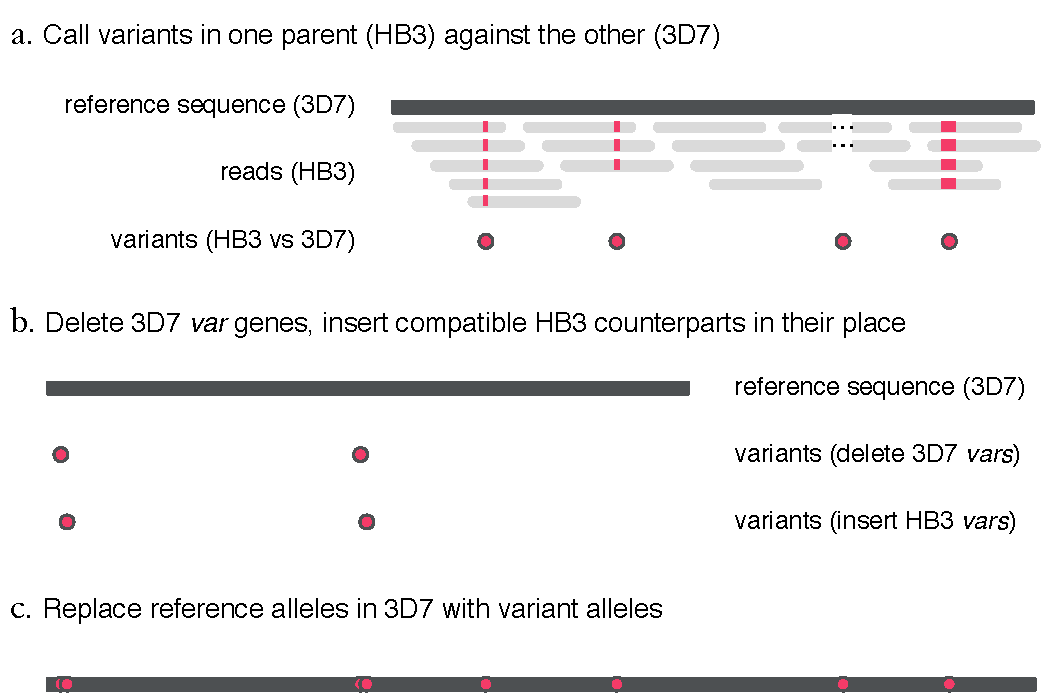
\includegraphics[width=\textwidth]{modrefworkflow}
  \caption{Workflow for generating the HB3 parental genome.  a. Reads from HB3 sample, PG0052-C, are mapped to the 3D7 reference genome, and variants (SNPs and indels) are called and stored as a VCF file.  b. We remove the 3D7 \textit{var} gene repertoire, replacing each with a reasonable HB3 \textit{var} counterpart, and encode the changes to the 3D7 reference genome as a VCF file.  c. We alter the reference genome using Algorithm \ref{alg:IncorporateVariantsIntoGenome}, thus producing the simulated HB3 genome.}
  \label{fig:modrefworkflow}
\end{figure}

We first obtained a VCF of variants found in the HB3 sample, PG0052-C, from the MalariaGen 3D7xHB3 cross dataset\cite{Miles:2015in}.  Variant counts are described in the Table \ref{tb:hb3_variants}, and include SNPs, insertions, deletions, and complex (simultaneous insertions and deletions) events.  These calls were made by combining the results of the reference-based \texttt{UnifiedGenotyper} module in the GATK\cite{DePristo:2011fo} and the reference-free bubble-calling algorithm in the Cortex\cite{Iqbal:2012fx} software.  All calls were restricted to the core genome; subtelomeric regions were masked out due to poor mapping properties (owing to the tremendous diversity in these regions of other \textit{P. falciparum} parasites with respect to the 3D7 reference).

\begin{table}[]
\centering
\caption{Variants found the HB3 (PG0052-C) sample from the MalariaGen 3D7xHB3 dataset.}
\label{tb:hb3_variants}
\begin{tabular}{@{}ccccc@{}}
\toprule
variants & SNPs   & insertions & deletions & complex \\
\midrule
42,054   & 15,376 & 11,807     & 14,643    & 228     \\
\bottomrule
\end{tabular}
\end{table}

Next, we produced a VCF describing \textit{var} gene replacements.  The sequences for HB3 \textit{var} genes and upstream promoter metadata were obtained from the VarDom server\cite{Rask:2010fi}.  No positional information from this data source is available, thus the exact placement of these \textit{var} genes in a chromosomal context is unclear.  However, previous work has established a strong association between conserved sequences of upstream promoters (phylogenetically grouped into five classes: A through E) and placement in the genome\cite{Kraemer:2006gv}.  We therefore replaced 3D7 \textit{var} genes with HB3 \textit{var} gene counterparts, taking care to replace genes with similar UPS classes whenever possible, and grouping genes with suspiciously incomplete metadata otherwise. The replacements were described in the resulting VCF as simultaneous deletions of the 3D7 allele and insertions of the HB3 allele.  No effort was made to match the orientation of the replacement \textit{var} gene with the replaced \textit{var} gene. The precise replacements are summarized in Table \ref{tb:hb3_vars}.

\begin{table}[]
\centering
\caption{\textit{Var} gene replacements from 3D7 to HB3 repertoire.}
\label{tb:hb3_vars}
\begin{tabular}{@{}llll@{}}
\toprule
3D7 gene & 3D7 ups class & HB3 gene & HB3 ups class \\
\midrule
PF3D7\_0421100 & UPSB5 & PFHG\_02500 & UNKNOWN \\
PF3D7\_0600200 & UPSB2 & PFHG\_02495 & UNKNOWN \\
PF3D7\_0632500 & UPSB5 & PFHG\_05132 & UNKNOWN \\
PF3D7\_0800300 & UPSB2 & PFHG\_04012 & ND \\
PF3D7\_1200400 & UPSB5 & PFHG\_05200 & ND \\
PF3D7\_1240900 & U     & PFHG\_05483 & ND \\
PF3D7\_0400400 & UPSA1 & PFHG\_03840 & UPSA1 \\
PF3D7\_0425800 & UPSA1 & PFHG\_03671 & UPSA1 \\
PF3D7\_1100200 & UPSA1 & PFHG\_04861 & UPSA1 \\
PF3D7\_1150400 & UPSA1 & PFHG\_05052 & UPSA1 \\
PF3D7\_1300300 & UPSA1 & PFHG\_03234 & UPSA1 \\
PF3D7\_0533100 & UPSA2 & PFHG\_03521 & UPSA2* \\
PF3D7\_0100300 & UPSA3 & PFHG\_02274 & UPSA3 \\
PF3D7\_0100100 & UPSB1 & PFHG\_04081 & UPSB1 \\
PF3D7\_0115700 & UPSB1 & PFHG\_04749 & UPSB1 \\
PF3D7\_0200100 & UPSB1 & PFHG\_03516 & UPSB1 \\
PF3D7\_0223500 & UPSB1 & PFHG\_04277 & UPSB1 \\
PF3D7\_0300100 & UPSB1 & PFHG\_03717 & UPSB1 \\
PF3D7\_0324900 & UPSB1 & PFHG\_04035 & UPSB1 \\
PF3D7\_0400100 & UPSB1 & PFHG\_04491 & UPSB1 \\
PF3D7\_0426000 & UPSB1 & PFHG\_04620 & UPSB1 \\
PF3D7\_0500100 & UPSB1 & PFHG\_04593 & UPSB1 \\
PF3D7\_0632800 & UPSB1 & PFHG\_04770 & UPSB1 \\
PF3D7\_0700100 & UPSB1 & PFHG\_04057 & UPSB1 \\
PF3D7\_0712300 & UPSB1 & PFHG\_03232 & UPSB1 \\
PF3D7\_0733000 & UPSB1 & PFHG\_04928 & UPSB1 \\
PF3D7\_0800100 & UPSB1 & PFHG\_03416 & UPSB1 \\
PF3D7\_0413100 & UPSB3 & PFHG\_03476 & UPSB3* \\
PF3D7\_0712400 & UPSB3 & PFHG\_02421 & UPSB3 \\
PF3D7\_1240300 & UPSB4 & PFHG\_02272 & UPSB4 \\
PF3D7\_0809100 & UPSB6 & PFHG\_02276 & UPSB6 \\
PF3D7\_0712800 & UPSB7 & PFHG\_04014 & UPSB7 \\
PF3D7\_0808700 & UPSB7 & PFHG\_02425 & UPSB7 \\
PF3D7\_1240400 & UPSB7 & PFHG\_04769 & UPSB7 \\
PF3D7\_0412400 & UPSC1 & PFHG\_03480 & UPSC1 \\
PF3D7\_0412700 & UPSC1 & PFHG\_03478 & UPSC1 \\
PF3D7\_0412900 & UPSC1 & PFHG\_00592 & UPSC1 \\
PF3D7\_0420700 & UPSC1 & PFHG\_02419 & UPSC1 \\
PF3D7\_0420900 & UPSC1 & PFHG\_02429 & UPSC1 \\
PF3D7\_0421300 & UPSC1 & PFHG\_02277 & UPSC1 \\
PF3D7\_0617400 & UPSC1 & PFHG\_02273 & UPSC1 \\
PF3D7\_0712900 & UPSC2 & PFHG\_04015 & UPSC2 \\
PF3D7\_1200600 & UPSE  & PFHG\_05046 & UPSE  \\
\bottomrule
\end{tabular}
\end{table}

These two VCFs were combined to produce a complete set of changes required to transform the 3D7 genome into a pseudo HB3 genome.  The transformation was applied using Algorithm \ref{alg:IncorporateVariantsIntoGenome}.

\section{Children}

Generating the genomes of the children is slightly more involved, as there is much more biology to simulate, and many more considerations to be made when placing variants. We generated VCF descriptions of the children using a multi-stage workflow shown in Figure \ref{fig:generatechildrenpipeline}.  In order, we simulate:

\begin{enumerate}
    \item homologous recombination between 3D7 and HB3 genomes
    \item gene conversion events
    \item NAHR events between compatible \textit{var} genes
    \item \textit{de novo} SNPs, insertions, deletions, and inversions
\end{enumerate}

\begin{figure}[h!]
  \centering
    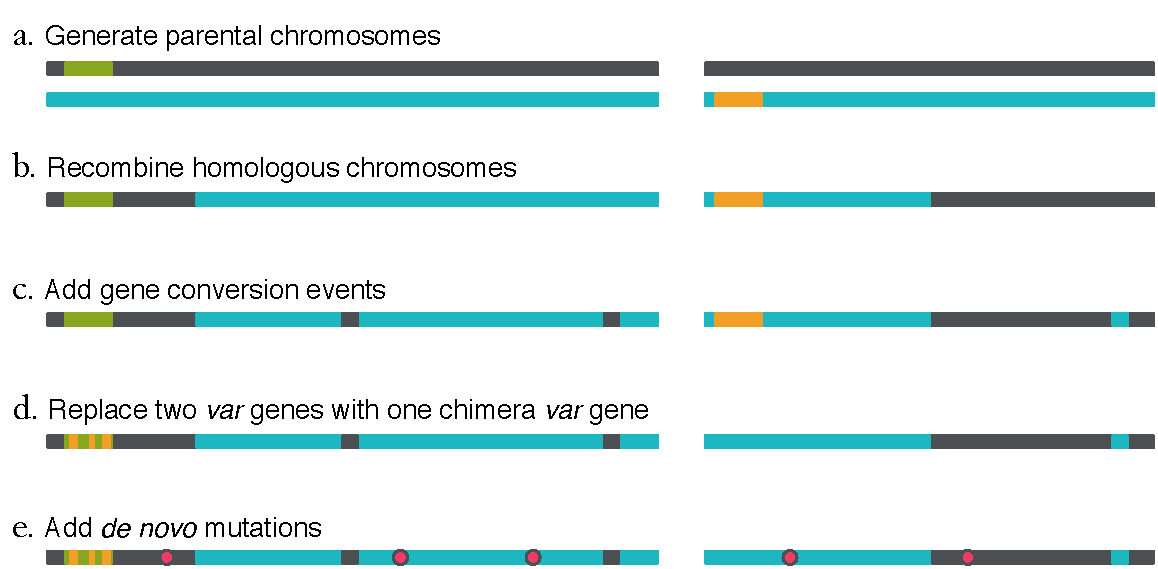
\includegraphics[width=\textwidth]{generatechildrenpipeline}
  \caption{Workflow for generating children's genomes.  a. Generate chromosomes from the parental genomes (compatible \textit{var} genes shown in green and orange).  b. Recombine homologous chromosomes.  c. Add gene conversion events (by incorporating variants from the alternative haplotypic background over a limited genomic window).  d. Replace one of the \textit{var} genes with a chimera of compatible genes.  e. Add \textit{de novo} mutations.}
  \label{fig:generatechildrenpipeline}
\end{figure}

\subsection{Homologous recombination}

\subsubsection{Allelic homologous recombination}

\begin{figure}[h!]
  \centering
    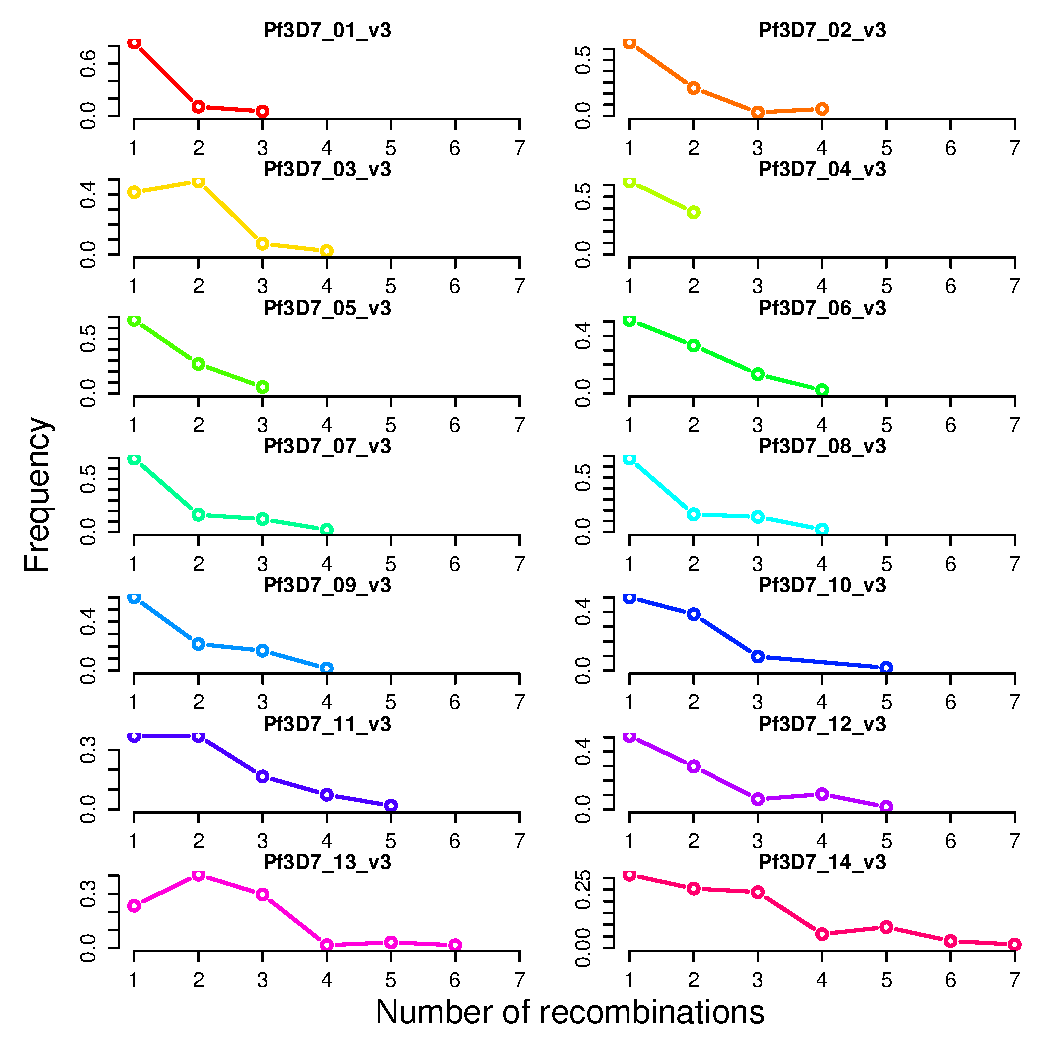
\includegraphics[width=\textwidth]{recomb-1}
  \caption{Empirical recombination frequencies per chromosome}
  \label{fig:recomb-1}
\end{figure}

For each bivalent chromosome, the cross-over rate will be dependent on the length of the chromosome. The empirical distributions for bivalent formation and crossover were generated from the $75$ samples in the MalariaGen crosses data. For each sample, only half of the chromosomes are expected to exhibit cross-over events.  The cross-over rates are plotted in Figure \ref{fig:recomb-1}. We simulated recombination in a sample by first drawing a binary number indicating whether a chromosome should be recombined, and if so, drawing the number of cross-over events per chromosome from these empirical distributions. The recombination sites themselves were chosen by drawing a uniform random variate between $1$ and the length of the chromosome. Although there are certainly hotspots and coldspots of recombination in the genome, we have ignored this complication.  An example haplotype mosaic of chromosome $12$ for five samples is shown in Figure \ref{fig:haplotypes12}.

\begin{figure}[h!]
  \centering
    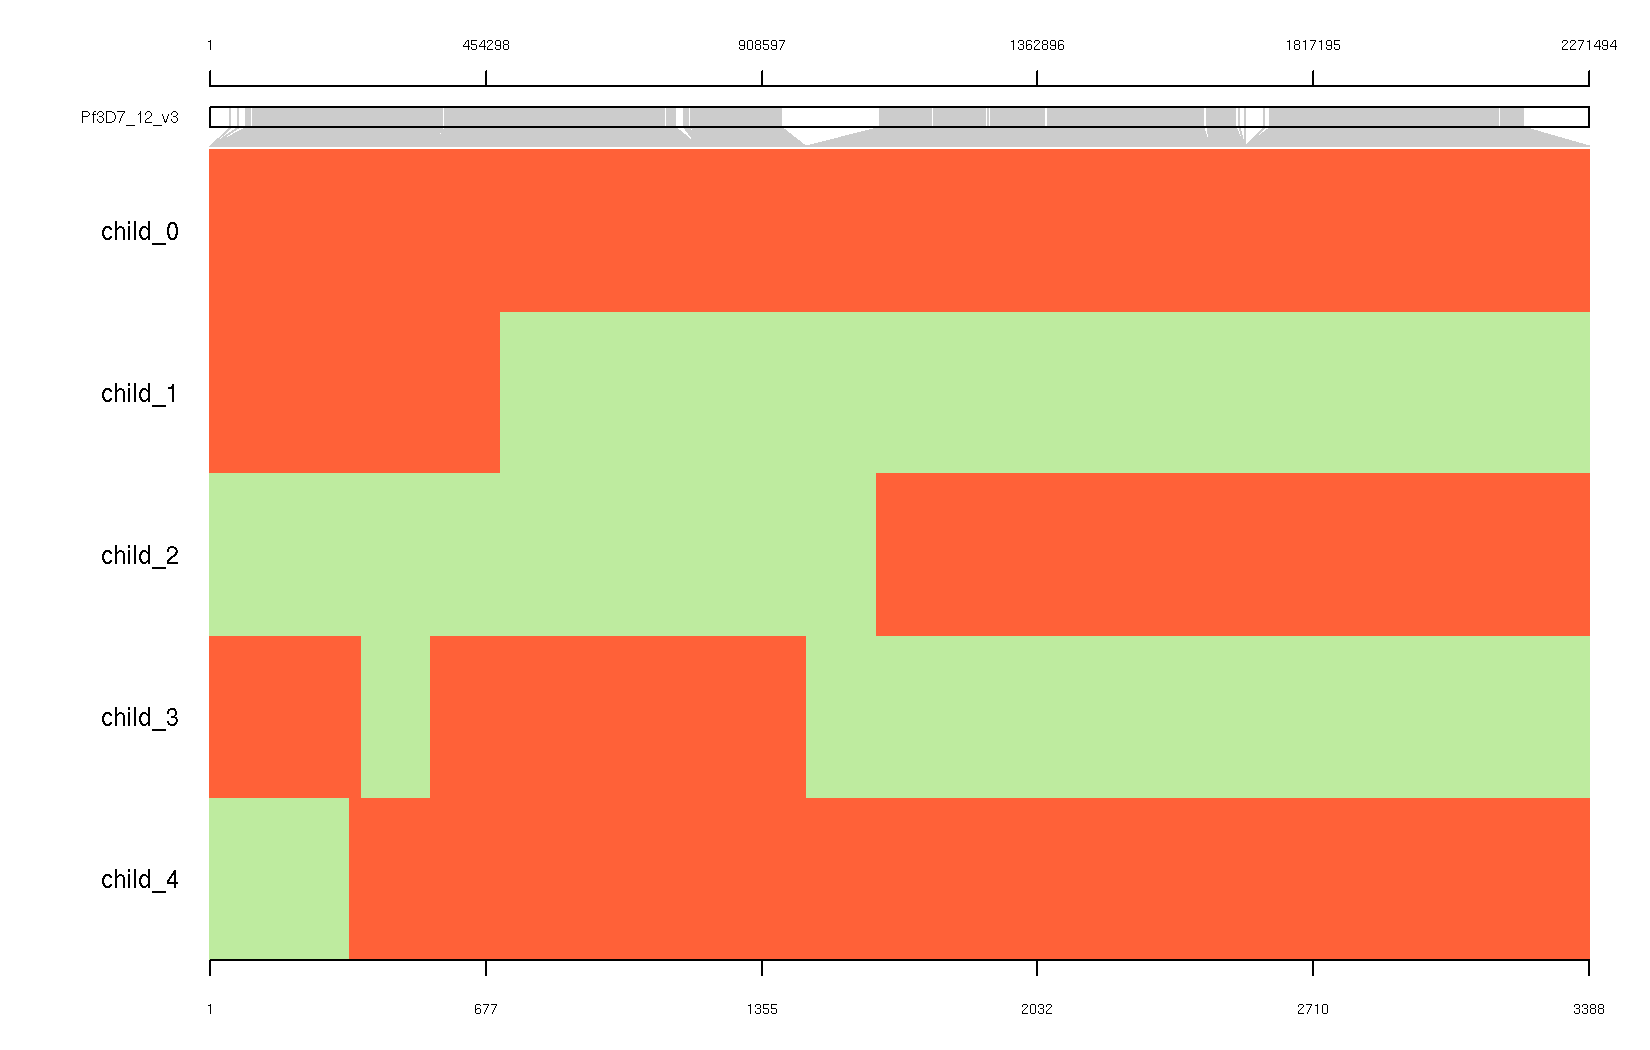
\includegraphics[width=\textwidth]{haplotypes12}
  \caption{Simulated haplotype mosaics for chromosome 12.  Genomic position is shown at the top of the figure, while variant number is shown at the bottom.  Each variant is depicted as a vertical grey line attached to the mosaic plot at the appropriate location.  In the mosaic, every variant is color-coded by parent of origin.}
  \label{fig:haplotypes12}
\end{figure}

\subsubsection{Gene conversion}

To simulate gene conversion events, we first chose a handful of random sites known to be variant in HB3, and determined the size of the event (number of adjacent HB3 variants involved in the gene conversion) by choosing a random uniform variate between $1$ and $3$. If these sites were originally transmitted to the child, they were removed from the VCF. If they had not been transmitted, they were added. The homologous recombinations and gene conversion events are displayed below for each chromosome and sample.

\subsubsection{Non-allelic homologous recombination}

NAHR events were generated by first finding compatible recombination partners. This list was generated by determining which 3D7 \textit{var} genes had been transmitted to the child, grouped by upstream promoter class and telomeric positioning ($5'$ or $3'$). In each group, two random genes were chosen. If necessary, the gene sequences were reverse complemented to have matching orientation (note that the sequences may not have the same orientation in the simulated genomes themselves). As NAHR events between two \textit{var} genes appear to occur in regions of homology, we identified shared $9$-mers, positioned between $20$ bp and $100$ bp between the two genes, to act as possible recombination sites. We randomly selected between $2$ and $5$ of these positions to act as recombination breakpoints, switching between the sequences and copied sequence data accordingly. Keeping in mind that our previous work has shown that the recombined \textit{var} genes are lost in order to produce the chimera, we added VCF records to delete the previous \textit{var} alleles from the child's genome and replace one of them with the recombined sequence.

\begin{figure}[h!]
  \centering
    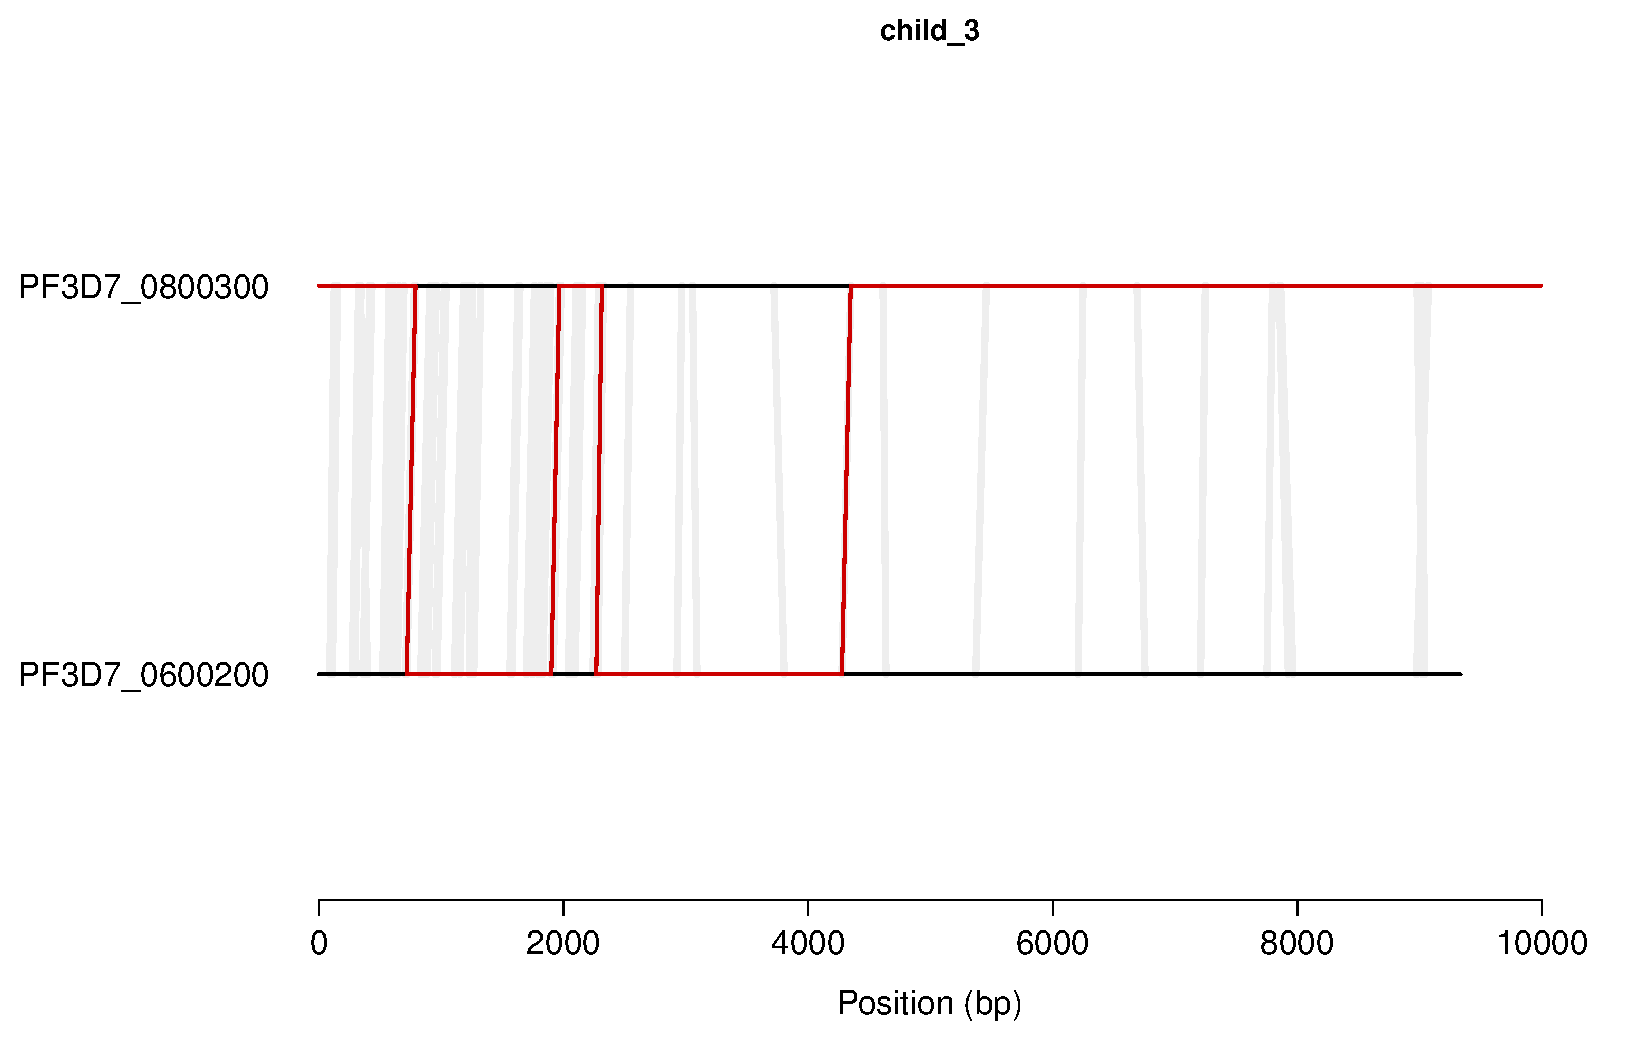
\includegraphics[width=\textwidth]{showrecomb-24}
  \caption{Non-allelic recombinations for two compatible \textit{var} genes.}
  \label{fig:showrecomb-24}
\end{figure}

\subsection{SNPs, insertions, and deletions}

\begin{figure}[h!]
  \centering
    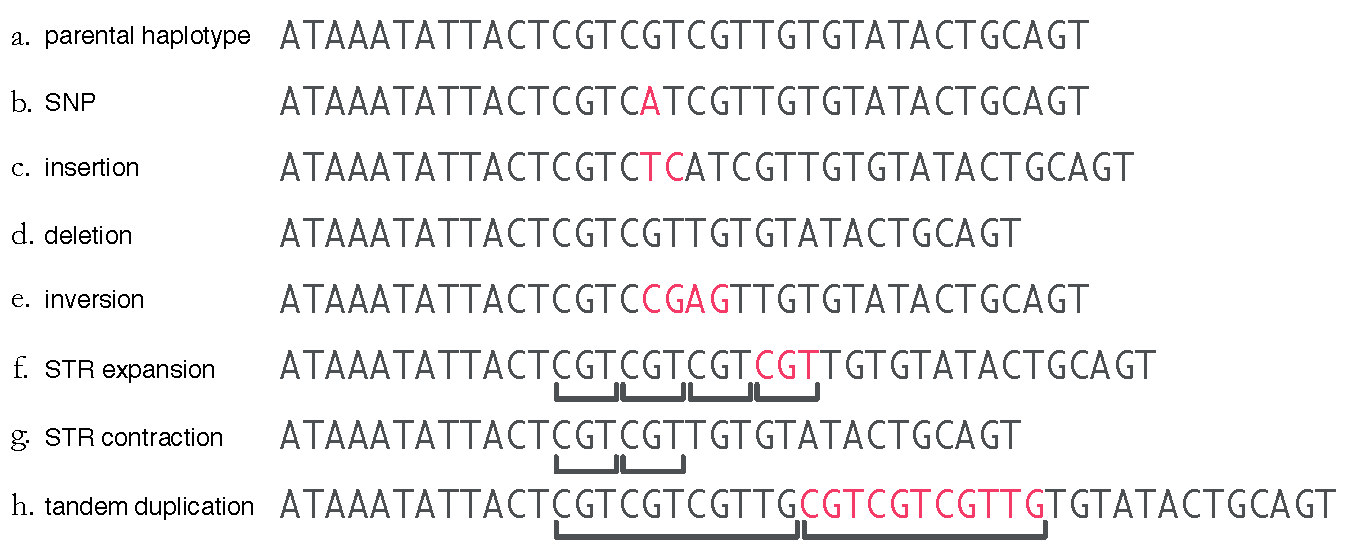
\includegraphics[width=\textwidth]{variants}
  \caption{Simulated variant types.  a. Original, parental haplotypic background upon which variants will be placed.  b. A single nucleotide polymorphism.  c. An insertion of two nucleotides.  d. A deletion of three nucleotides.  e. An inversion of four nucleotides.  f. Expansion of a $3$ bp short tandem repeat (STR) by one unit.  g. A contraction of an STR by one unit.  h. A tandem duplication of $11$ nucleotides.}
  \label{fig:variants}
\end{figure}

With the ground state genome now generated, we further generated simple events - SNPs, insertions, and deletions - on this foundation to complete the production of the child's genome.  The precise number of events can be specified by the user at runtime, and for each simulated genome, different counts were specified.

To simulate \textit{de novo} SNPs, we added sites with random (non-reference) alleles at random positions throughout the genome.  We also simulated insertion, deletion, and inversion events at every length between $1$ and $100$ bp. For insertions, random alleles were generated and tested to ensure they did not match the allele already in the reference sequence. For deletions, we simply replaced the reference allele with a truncated allele of the prescribed length. For inversions, we replace the reference allele with its complement.

\subsubsection{Expansion and contraction of short tandem repeats (STRs)}

As a special case of indels, we sought specifically to simulate the expansion and contraction of short tandem repeats (STRs), depicted in Figure \ref{fig:variants}f-g. STRs are constrained to occur at loci where there are already existing repeats, and expansions (contractions) should manifest as the insertion (deletion) of whole units at a time.  We first built a map of repeated $2$-bp, $3$-bp, $4$-bp, and $5$-bp sequences in the 3D7 genome. We filtered these lists, retaining only STRs where the repeated unit occurred at least three times. For each simulated event, we randomly chose a position from the appropriate list and select a number of units to add or remove. The number of units is constrained to be less than the length of the number of repeat units of the existing STR. With these considerations, we simulated expansions and contractions at the aforementioned repeat unit sizes.

\subsubsection{Tandem duplications}

For tandem duplications (as depicted in Figure \ref{fig:variants}h) of length $l$, we chose positions in the genome at random, copied the next $l$ bases, and inserted an identical copy at the same locus.  Events at each length between $10$ bp and $50$ bp were produced.

\section{Simulating reads}

We now turn our attention to simulating second-generation sequencing reads given an underlying genome.  There are existing tools that will simulate perfect reads and uniform coverage, which will be important for initial tests of our variant identification software.  However, the crucial simulation is of imperfect reads with non-uniform coverage.  Without this, any estimate of our sensitivity and specificity is unlikely to be predictive of performance in real data.

There are many tools that can simulate imperfect reads from a given sequence.  Almost every solution involves user-specified parameters controlling the properties of the sequencing data.  For instance, a tool may model fragment size as a normal distribution, requiring the user to specify the requisite shape parameters.  It may also permit the user to specify a desired mismatch rate to simulate the presence of sequencing error.  Some tools have presets that automatically set parameters to those consistent with average behavior for various sequencing platforms.

The problem with all of these tools is an over-reliance on assumed parameters of real data.  Should a fragment size distribution for real data deviate from the typical normal distribution, this will not be captured in the simulated dataset.  Mismatch and indel errors do not happen at any position in the read with equal probability, but rather are biased towards later cycles and certain sequence contexts.  Read coverage is not simply Poisson-distributed, but varies across the length of the genome depending on GC bias, secondary structure, even the particular sequencing chemistry used.  There are currently no tools that are capable of capturing such nuance.

Instead, we chose to learn empirical distributions of major sequencing properties using an exemplar dataset and sample from those distributions directly in order to generate reads.  This frees us from having to make any assumptions about our dataset, easily generalizes to any dataset regardless of when, where, or how it was sequenced.  It's also vastly more realistic than other approaches.

Our approach is detailed below.  Briefly, it consists of three components:

\begin{enumerate}
    \item A "coverage profile": a description of where every fragment and read in the genome should fall and which should contain errors.
    \item A "read profile": a description of where to place errors within a read, including mismatches, insertions, and deletions.
    \item The read simulator: samples from the profiles to generate reads in the new reference sequence.
\end{enumerate}

\subsection{Constructing the coverage profile}

Construction of a coverage profile consists of two sub-problems: providing a complete description of where reads fall on the existing reference sequence, and transferring that information sensibly to the modified reference sequence.  This is depicted in Figure \ref{fig:coverageprofile}.  We address each of these needs with custom tools.

\begin{figure}[h!]
  \centering
    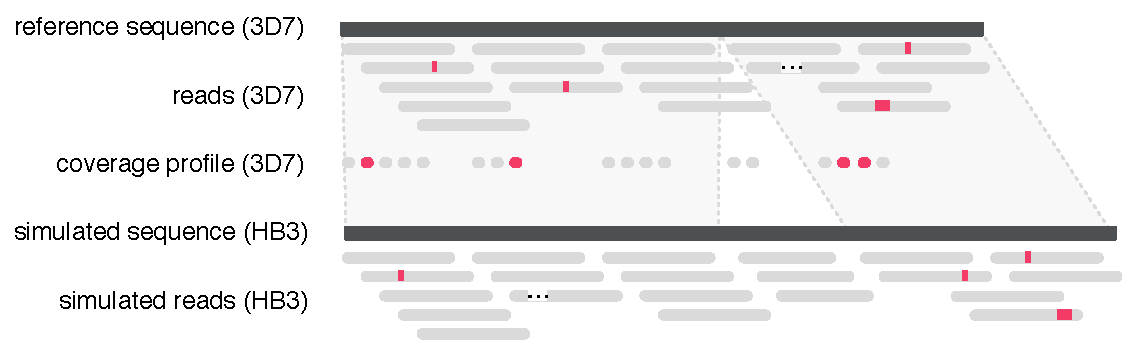
\includegraphics[width=\textwidth]{coverageprofile}
  \caption{Construction of the coverage profile for the reference genome and liftover to the altered genome.  Each read start (and fragment start, not shown) is stored along with a count of the number of reads at that location that contain errors.  This information is then lifted over to the simulated sequence, and gaps in the table are filled in with neighboring values.}
  \label{fig:coverageprofile}
\end{figure}

\subsubsection{Computing read and fragment starts, and error rates}

We developed a tool, \texttt{ComputeBaseAndFragmentErrorRates}, which provides a precise specification for the number of fragments and reads found starting at of every position in the canonical reference genome, as well as an accounting as to which reads and fragments contained any kind of error (mismatch or indels).  Briefly, we iterate over every chromosome in the reference genome, advancing through every aligned read stored in an exemplar sample's coordinate-sorted BAM file.  We instantiate a chromosome-length array indicating the number of reads that start at a given position and the number of reads that contain apparent errors (any discrepancy from the reference sequence).

We must also store information about read fragment starts and error rates, which requires us to keep track of read pairs as we traverse the BAM file.  To do so, we hash the read name to the first instance of the read we see along the length of a chromosome.  As paired-end reads have the same name, the second time we see the same read name, we will have found the second end of the pair.  We then increment the count at the chromosome array position that corresponds to the $5'$-most end of the pair, and increment the fragment errors array based on errors in either end of the pair.

This algorithm is described in Algorithm \ref{alg:ComputeBaseAndFragmentErrorRates}.

\begin{algorithm}
\caption{Emit all fragment starts, read starts, and error rates per position.}
\label{alg:ComputeBaseAndFragmentErrorRates}
\begin{algorithmic}[1]
\Function{ComputeBaseAndFragmentErrorRates}{BAM}
    \ForAll{$\textit{chr} \textrm{ in } \textit{chrs}$}
        \State $\textit{nReadsErrors} \gets []$
        \State $\textit{nReads} \gets []$
        \State $\textit{nFragmentsErrors} \gets []$
        \State $\textit{nFragments} \gets []$
        \State $\textit{seenReads} \gets []$

        \State $\textit{reads} \gets \textit{BAM.getAllReads(chr)}$

        \ForAll{$\textit{read} \textrm{ in } \textit{reads}$}
            \State $\textit{readErrorPositions} \gets \textit{getPositionsErrors(read)}$
            \State $\textit{refErrorPositions} \gets \textit{convertReadPositionsToReferencePositions(readErrorPositions)}$

            \ForAll{$\textit{refErrorPosition} \textrm{ in } \textit{refErrorPositions}$}
                \State $\textit{nReadsErrors[refErrorPosition]}++$
            \EndFor

            \For{$\textit{readPosition} \textrm{ in } 0:\textit{read.length()}$}
                \State $\textit{nReads[convertReadPositionsToReferencePositions(readPosition)]}++$
            \EndFor

            \If{$\textit{!seenReads.contains(read.getName())}$}
                \State $\textit{seenReads} \gets \textit{read.getName()}$
            \Else
                \State $\textit{mateErrorPositions} \gets \textit{getPositionsErrors(seenReads[read.getName()])}$

                \If $\textit{readErrorPositions.size()} + \textit{mateErrorPositions.size()} \ge 1$
                    \State $\textit{nFragmentsErrors[seenReads[read.getName()].getAlignmentStart()}++$  
                \EndIf

                \State $\textit{nFragments[seenReads[read.getName()]}++$  
            \EndIf
        \EndFor

        \For{$\textit{pos} \textrm{ in } 0:\textit{nReads.length()}$}
            \State $\textit{print chr, pos, nReadsErrors[pos], nReads[pos], nFragmentsErrors[pos], nFragments[pos]}$
        \EndFor
    \EndFor
\EndFunction
\end{algorithmic}
\end{algorithm}

\subsubsection{Lifting read profile over from reference to simulated genome}

The genomic coordinates present in the table produced by Algorithm \ref{alg:ComputeBaseAndFragmentErrorRates} must be transformed from the reference sequence to the simulated genome before it can be used.  To do so, we developed a tool that could liftover the coordinates appropriately when given the table, reference sequence, and a VCF file describing the alterations made to the reference to transform it into the simulated genome.  This is accomplished with an algorithm similar to Algorithm \ref{alg:IncorporateVariantsIntoGenome}.  We iterate through each chromosome as we did before, storing the entire sequence as an array of strings, placing alternate alleles in the place of reference alleles, or in the case of deletions, replacing reference alleles with blank strings.  Once the array is populated, we advance through the coverage table one position at a time.  At each position, we emit the contents of the previously constructed table with the number of reads, fragments, and errors for each.  At some positions, insertions will have changed the length of the sequence in the bin, and the extra positions will not have explicit read and fragment information to emit.  To account for this, we keep running statistics on previously seen read and fragment statistics from which we can compute running means and standard deviation.  We generate new values for the number of reads, fragments, and error rates as necessary as the mean plus standard deviation of the relevant metric, ensuring the values are never less than $0$, and that we round up or down to the nearest integer (error rates are rounded up and read/fragment counts are rounded down to increase our self-penalty).

This algorithm is described in \ref{alg:LiftoverFromRefToChild}.

\begin{algorithm}
\caption{Lift a table from reference to child coordinates.}
\label{alg:LiftoverFromRefToChild}
\begin{algorithmic}[1]
\Function{LiftoverFromRefToChild}{ref, vcf, table}
    \ForAll{$\textit{chr} \textrm{ in } \textit{ref}$}
        \State $\textit{newchr} = \textit{IncorporateVariantsIntoGenome(ref, vcf)}$

        \For{$i \textrm{ in } 0:newchr.length()$}
            \State $\textit{emit(table[i])}$
            \If{$newchr[i].length() > 1$}
                \For{$j \textrm{ in } 1:newchr[i].length()$}
                    \State $\textit{emit(extrapolate(table[i]))}$
                \EndFor
            \EndIf
        \EndFor
    \EndFor
\EndFunction
\end{algorithmic}
\end{algorithm}

\subsection{Constructing the read profile}

Next, we generate the read profile, describing the various properties of fragments and read.  As in previous examples, we iterate over each read in the exemplar sample's BAM file, storing relevant information in tabular form.

\subsubsection{Scalar properties}
We first store the following scalar information (as the data we are modelling is assumed to be Illumina data generated from a single library, some properties which could otherwise be stored as distributions are instead treated as a single number that will be simple constants in our simulation):

\begin{enumerate}
    \item read length
    \item number of reads
    \item number of reads with errors
    \item number of read pairs
    \item number of chimeric pairs (each end aligned to different chromosomes)
    \item number of mismatches 
    \item number of insertions
    \item number of deletions
\end{enumerate}

Example values for each of these metrics can be found in Table \ref{tbl:scalarvalues}.  Note that some of the mismatches, insertions, and deletions may represent true variation between the sample and the reference sequence.  We do not mask these sites out.  While this increases the apparent error rate, the variant rates are typically low compared to the number of bases in the reference sequence itself, making the difference negligible.  Furthermore, we will choose the reference sample as the exemplar dataset for the read simulations.  Since this sample should theoretically be identical to the reference sequence, this choice obviates the need for any masking of variants in the reference sample against the reference sequence.

\begin{table}[]
\centering
\caption{Example read and fragment scalar properties for sample PG0063-C.}
\label{tbl:scalarvalues}
\begin{tabular}{@{}lr@{}}
\toprule
                   & PG0051-C\\
\midrule
readLength         & 76\\
numReads           & 38,846,418\\
numReadsWithErrors & 3,696,708\\
numPairs           & 19,473,634\\
numChimericPairs   & 348,294\\
numMismatches      & 6,525,504\\
numInsertions      & 139,941\\
numDeletions       & 317,076\\
\bottomrule
\end{tabular}
\end{table}

\subsubsection{Empirical distributions}

Other properties take on a range of values with some probability.  Rather than trying to fit the underlying distributions explicitly (which can often fail as datasets contain more nuance than what sequencing platforms should theoretically produce), we instead store empirical distributions and generate random values from them accordingly.  We store the following empirical distributions:

\begin{enumerate}
    \item number of errors (of any type - mismatch, insertion, or deletion) in a read
    \item fragment size
    \item insertion size
    \item deletion size
\end{enumerate}

Note that these distributions are not conditioned on position in the read.  Example distributions derived from an exemplar sample are shown in Figure \ref{fig:empDists-1}.

\begin{figure}[h!]
  \centering
    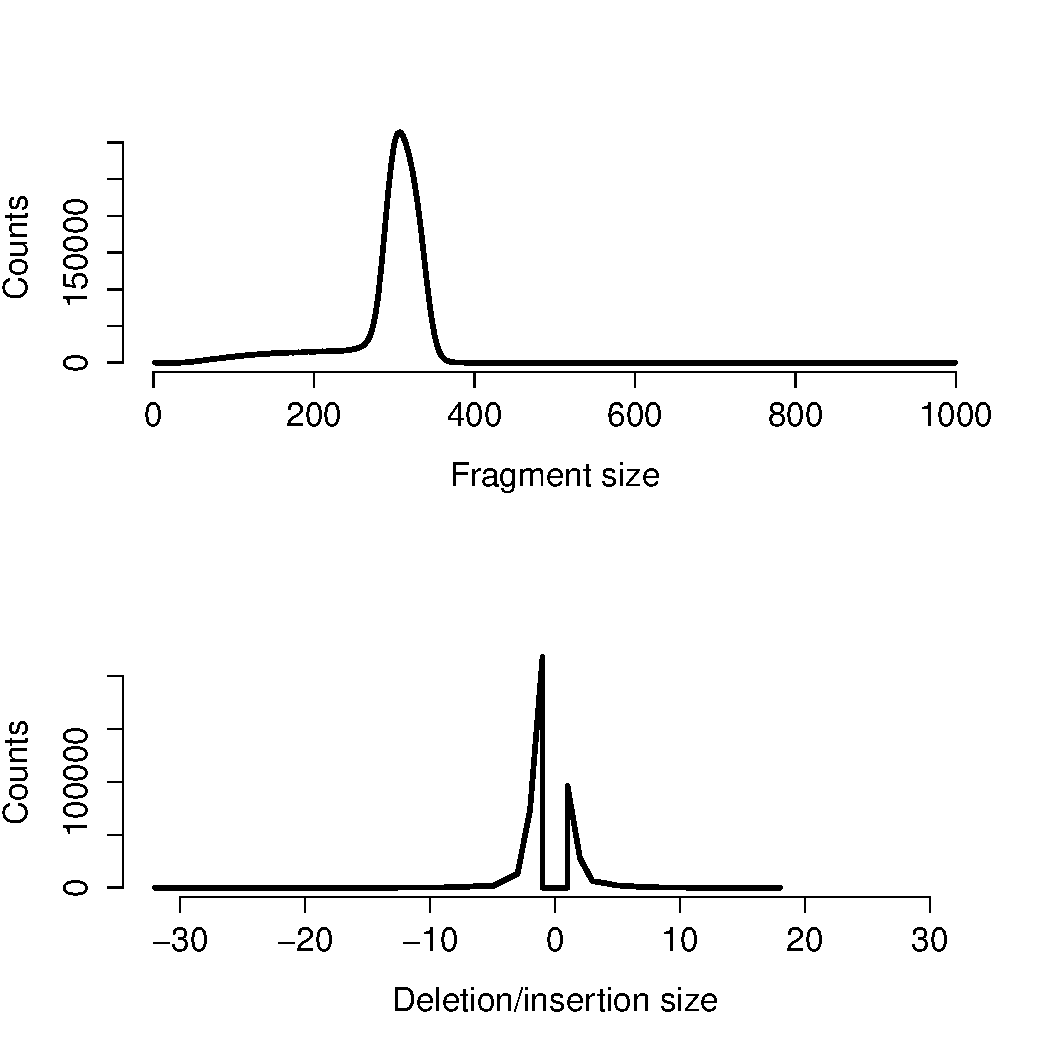
\includegraphics[width=\textwidth]{empDists-1}
  \caption{Top: empirical fragment size distribution for PG0051-C.  Bottom: empirical deletion (negative values) and insertion (positive values) length distribution for the same sample.}
  \label{fig:empDists-1}
\end{figure}

\subsubsection{Covariate table}

Finally, we construct the covariate table: a set of empirical distributions for various error events conditioned on the following:

\begin{enumerate}
    \item type (SNP, insertion, deletion)
    \item end of pair (first end or second end)
    \item strand (positive or negative)
    \item $5'$ dinucleotide context
    \item position in read
    \item first base of error sequence (empty for deletions)
\end{enumerate}

For each read, we increment an element in a table that corresponds to these six covariates.  The code to do so is contained in our \texttt{GenerateReadSimProfile} module.

\subsection{The read simulator}

With the coverage and read profiles in hand, we are finally ready to simulate reads.  We advance through each base of the simulated genome, reading the coverage profile as we traverse.  At each site, we use the coverage profile to dictate the number of fragments that must be generated and how many of those fragments should contain errors, thus modelling regions of the genome with higher or lower error rates.  We then generate fragments, sampling fragment lengths from the empirical fragment length distribution.  If a read is to contain an error, as specified by the coverage profile, we construct a read-specific error profile for mismatches, insertions, and deletions.  These profiles take into account the preceeding dinucleotide context for each position in the read\footnote{To handle the first and second positions in the read, which do not have a dinucleotide context, we simply extract a read by starting two nucleotides into the simulated fragment.}, the end of the pair being simulated, whether the fragment came from the positive or negative strand, and the first nucleotide of the error to be incorporated (not applicable for deletions).  

\begin{sidewaysfigure}[h!]
  \centering
    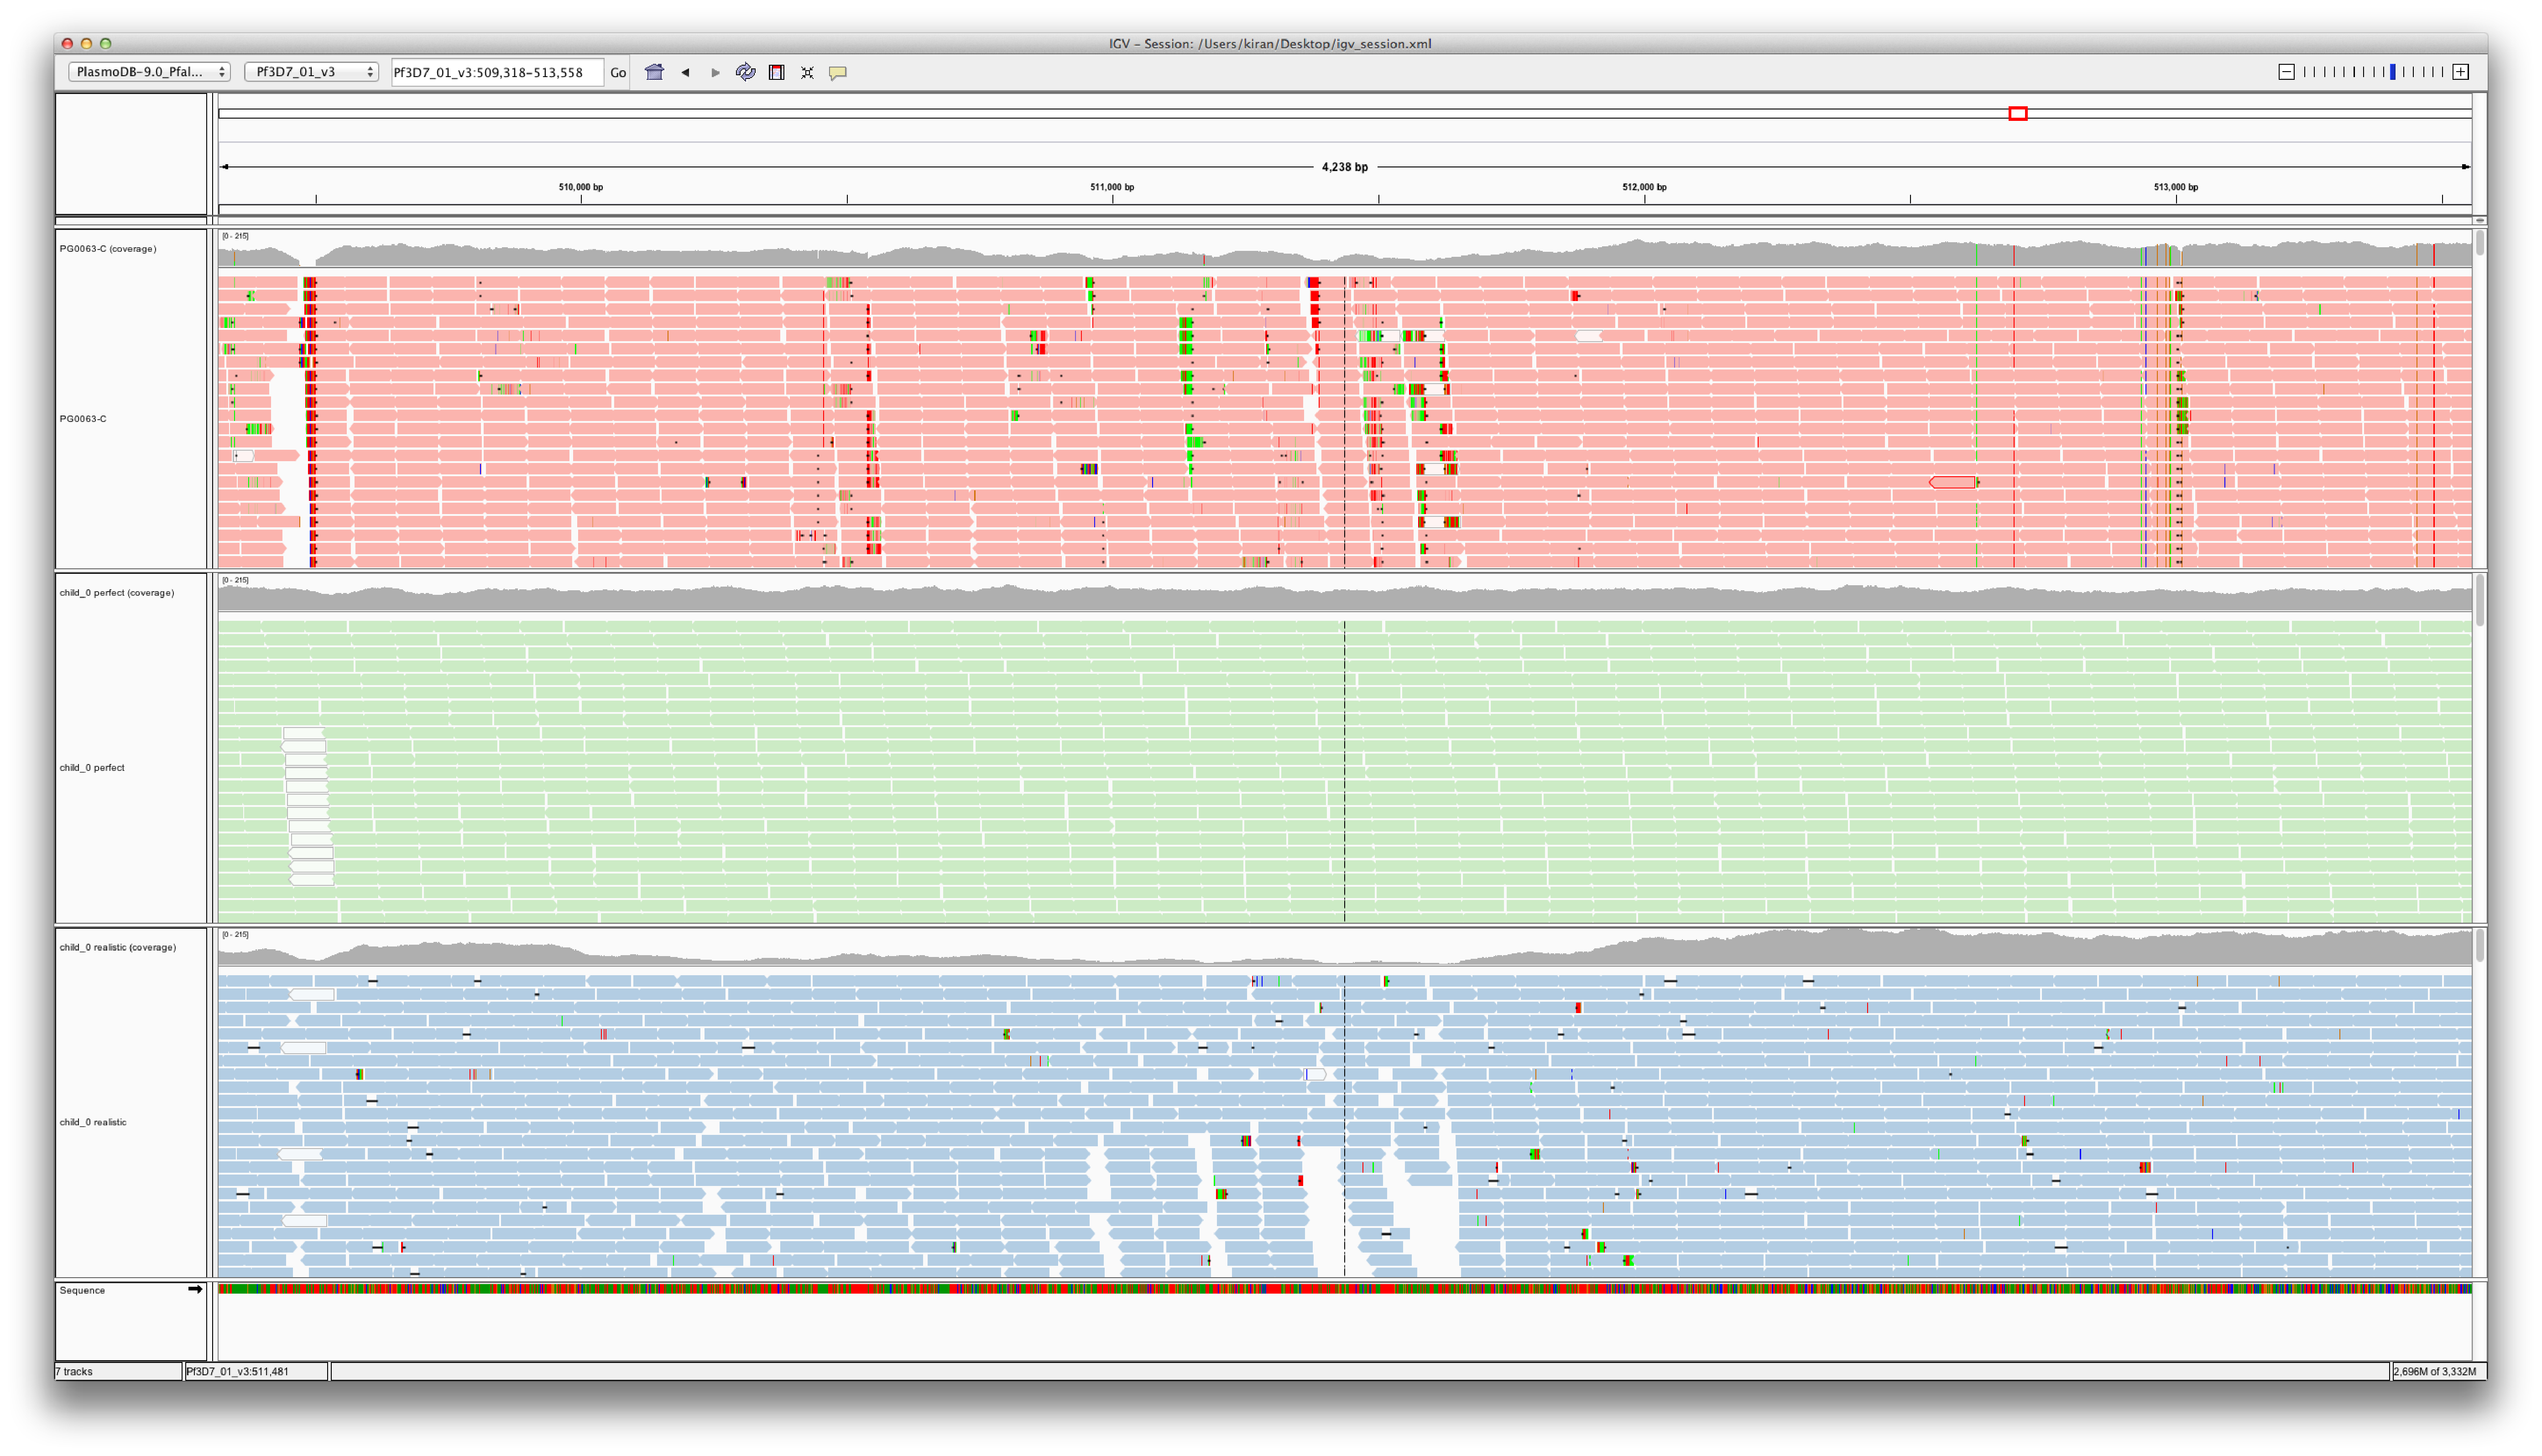
\includegraphics[width=\textwidth]{simreads}
  \caption{Read datasets for real (top panel), simulated perfect (middle panel), and simulated realistic (bottom panel) data.}
  \label{fig:simreads}
\end{sidewaysfigure}

\section{The simulated dataset}

With our genome and read simulation framework now complete, we simulated the genomes of $20$ progeny from a pseudo 3D7xHB3 cross.  The precise counts of variant types per sample are shown in Table \ref{tb:simstats}.  For each sample, we generated two datasets: a so-called "perfect" dataset (uniform coverage, perfect reads), and a so-called "realistic" dataset (non-uniform coverage, imperfect reads).  Both datasets contain approximately $150x$ coverage.

\begin{table}[]
\centering
\caption{\textit{De novo} variant counts for each of the $20$ simulated children.}
\label{tb:simstats}
\begin{tabular}{lrrrrrrrrrr}
\toprule
  & DEL & GC & INS & INV & NAHR & RECOMB & SNP & STR\_CON & STR\_EXP & TD\\
\midrule
0 & 22 & 25 & 22 & 22 & 2 & 10 & 5 & 3 & 3 & 26\\
1 & 21 & 21 & 21 & 21 & 2 & 10 & 23 & 11 & 11 & 26\\
2 & 11 & 22 & 11 & 11 & 2 & 8 & 13 & 22 & 22 & 8\\
3 & 25 & 17 & 25 & 25 & 2 & 32 & 23 & 17 & 17 & 21\\
4 & 4 & 23 & 4 & 4 & 2 & 8 & 14 & 16 & 16 & 12\\
5 & 26 & 23 & 26 & 26 & 2 & 37 & 28 & 5 & 5 & 8\\
6 & 13 & 17 & 13 & 13 & 2 & 15 & 27 & 23 & 23 & 4\\
7 & 1 & 22 & 1 & 1 & 2 & 30 & 28 & 5 & 5 & 12\\
8 & 26 & 16 & 26 & 26 & 2 & 16 & 16 & 13 & 13 & 8\\
9 & 4 & 23 & 4 & 4 & 2 & 25 & 23 & 23 & 23 & 21\\
10 & 12 & 20 & 12 & 12 & 2 & 16 & 23 & 19 & 19 & 27\\
11 & 13 & 19 & 13 & 13 & 2 & 7 & 20 & 18 & 18 & 17\\
12 & 19 & 20 & 19 & 19 & 2 & 8 & 14 & 5 & 5 & 28\\
13 & 10 & 20 & 10 & 10 & 2 & 25 & 13 & 28 & 28 & 11\\
14 & 28 & 18 & 28 & 28 & 2 & 8 & 3 & 29 & 29 & 17\\
15 & 27 & 22 & 27 & 27 & 2 & 30 & 5 & 19 & 19 & 2\\
16 & 23 & 22 & 23 & 23 & 2 & 12 & 29 & 24 & 24 & 17\\
17 & 17 & 22 & 17 & 17 & 1 & 10 & 28 & 13 & 13 & 11\\
18 & 23 & 18 & 23 & 23 & 2 & 8 & 1 & 21 & 21 & 18\\
19 & 22 & 22 & 22 & 22 & 2 & 17 & 19 & 3 & 3 & 2\\
\bottomrule
\end{tabular}
\end{table}

\section{Summary}

Unlike many other genome and read simulation software packages, our framework is able to generate realistic genomes and reads that exhibit allelic recombinations, non-allelic recombinations, a wide (and tuneable) spectrum of \textit{de novo} variants, and reads with realistic sequencing properties.  Rather than requiring a user to specify recombination rates, coverage levels, insert size distributions, and sequencing error rates (all of which may deviate wildly from real data), we have adopted the point of view that the end goal is to simulate data similar to a dataset one already possesses.  By drawing from empirical distributions derived from real data, we should find that the performance of our software on simulated data is informative of its capabilities on real data.

We do note a minor error in our simulation.  When producing empirical distributions for the lengths of indel errors, we treated insertions and deletions as separate events needing separate distributions.  However, inspecting these distributions more closely, we notice a bias: more deletion errors are present than insertion errors.  This is likely to be an artifact of read mapping, rather than of biology or even of sequencing.  Reads with insertions are typically more troublesome to place on a reference genome correctly than reads with deletions.  Still, it would have been more appropriate to sample insertion and deletion error lengths from the same distribution.  This error is not expected to compromise the results from the simulation.

We also note a deliberate omission: sample contamination.  Sample contamination by non-\textit{P. falciparum} data could generate false positive calls if, for instance, a child's sample is contaminated but the parents are not.  This point will be discussed in greater detail when examining validation data in Chapter \ref{cg:realdata}.

\chapter{Detection and classification}
\label{ch:methods}

\newthought{We now present a novel graphical method} for detecting and classifiying \textit{de novo} variants.  We shall present some brief foundational background on \textit{de novo} assembly and graphical models, concepts upon which the variant caller is built.  The simulation framework and dataset we described in Chapter \ref{ch:simulation} will be used to establish the method's accuracy.

Reference-based analyses benefit from being reasonably intuitive, as the underlying genome is linear and there are many visualization tools that can facilitate the user's understanding of the underlying data\cite{Li:2009p181,Bao:2009ie,Robinson:2011gy,Milne:2013gf,Thorvaldsdottir:2013iw}.  In contrast, graph data structures are far less intuitive and lack dedicated visualization tools in the genomics space.  In this chapter, we will also present images from our purpose-built graph visualization software for the purposes of guiding the reader's intuition regarding graphical variant motifs and the operation of the calling algorithms.

\section{\textit{De novo} assembly}

\textit{De novo} assembly refers to the process wherein a sampled genome is reconstructed from sequencing data without guidance from an existing genome.  Sequenced deeply enough, a set of reads from a single sample will contain overlaps that can be used to infer the sequence of contiguous segments of the genome into so-called \textbf{contigs}.  If the reads are long enough to span repetitive regions in the genome, these contigs could be as long as the chromosome itself.  Otherwise, separate contigs can be joined together into \textbf{scaffolds} (contigs plus gaps) using paired-end reads, long reads, information from linkage analysis, Hi-C data\cite{Burton:2013dj}, or other methods.

The quality of the reconstruction can vary considerably depending on how the assembly is performed.  Typically, constructing a complete and high-quality reference sequence (one with few errors and few gaps in the linear sequence of each assembled chromosome) is a big first step to studying the genome of an organism, done at great expense and labor over a period of several years.  In 2002, after several years of work, Gardner \textit{et al.} published the sequence of the 3D7 \textit{P. falciparum} parasite clone.  By using a whole chromosome shotgun strategy with accurate and long (several hundred bp) first-generation sequencing reads (Sanger), each chromosome was fully resolved with very few gaps in the sequence and no unplaced contigs\cite{Gardner:2002p1564}.

Today, the same sample can be assembled in a matter of days rather than years using high-throughput second-generation sequencing.  Short reads ($76-100$ bp) from second-generation sequencers (Illumina) can be produced cheaply and in abundant quantities, and similar read overlap considerations can be used to generate assemblies.  However, these reads tend to be much more error prone, and the shorter read length fails to span many repetitive regions of the genome.  The result is a much cheaper, but far more fragmented assembly than the reference assembly.  Table \ref{tbl:asmcompare} compares the assembly statistics of the reference genome versus a reconstruction of the same sample from Illumina data taken from our cross dataset (PG0051-C) using the McCortex assembly software\cite{Turner:2015ve}.  While the parasite genome is known to have $16$ chromosomes (which the reference recapitulates), the Illumina assembly broken into over $50,000$ pieces with an N50\footnote{\textbf{N50}: the length for which the set of all contigs that length or greater represents half the total lengths of all contigs.} of a mere $1,280$ bp.

\begin{table}[]
\centering
\caption{Comparison of assembly statistics of the finished 3D7 reference genome and a reconstruction of the same sample from $76$-bp Illumina data.}
\label{tbl:asmcompare}
\begin{tabular}{@{}lllllll@{}}
\toprule
          & contigs & min length & max length & mean length & N50     & total sequence \\ \midrule
3D7       & 16      & 5967       & 3291936    & 1458302     & 1687656 & 23332831       \\
PG0051-C  & 51425   & 47         & 27520      & 478         & 1280    & 24602599       \\ \bottomrule
\end{tabular}
\end{table}

It is perhaps surprising then to discover the central argument of this dissertation is on the value of \textit{de novo} assembly of short reads for \textit{de novo} mutation discovery.  After all, a poor-quality Illumina assembly - as evidenced by the numerous short contigs - would seem to be very limiting, even if it could theoretically reconstruct pieces of the genome that cannot be recovered from a reference-based analysis.  However, for the work that we describe in this chapter, the value is not in the contig reconstructions, but in the underlying data structure from which the contigs are produced: the "de Bruijn graph".

The de Bruijn graph is a data structure that encodes read overlaps such that a walk through the vertices with unambiguous connections yields contiguous sequence in the genome.  In real data, those walks may end prematurely due to errors or homology, yielding junctions that cannot be confidently navigated.  Typically, assembly algorithms will be conservative in the contigs they emit from this data, choosing to terminate the walk at the junction rather than risk going forward and emitting sequence that does not actually appear in the genome.  However, with an additional set of metadata and a reasonable assumption, we can traverse the barrier.  In trio data, it is easy to detect a so-called novel kmer: a kmer occuring in the child but absent in the parents.  By annotating the graph with this information, we can see stretches of novel kmers.  Figure \ref{fig:graphwithextras} shows a portion of such an annotated graph.  Ignoring the annotations, a traversal that starts at vertex $D$ would yield a short contig: $C \rightarrow D \rightarrow E$.  However, if we assume the novel kmers link together, we can extend our traversal to yield $C \rightarrow D \rightarrow E \rightarrow F \rightarrow G \rightarrow H$.  These novel kmers are the hallmark of \textit{de novo} variation, and by utilizing these annotations, we can navigate parts of the graph that are otherwise unnavigable, surpassing what conservative contigs can give us and providing tremendous sensitivity and specificity to DNMs.

\begin{figure}[h!]
  \centering
    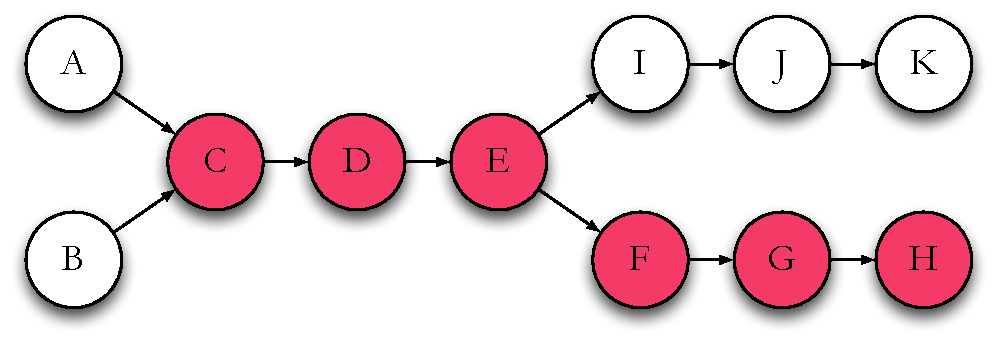
\includegraphics[width=0.8\textwidth]{graphwithextras}
  \caption{Graph with novel kmer annotations in red.}
  \label{fig:graphwithextras}
\end{figure}

\subsection{Definitions}

\begin{figure}[h!]
  \centering
    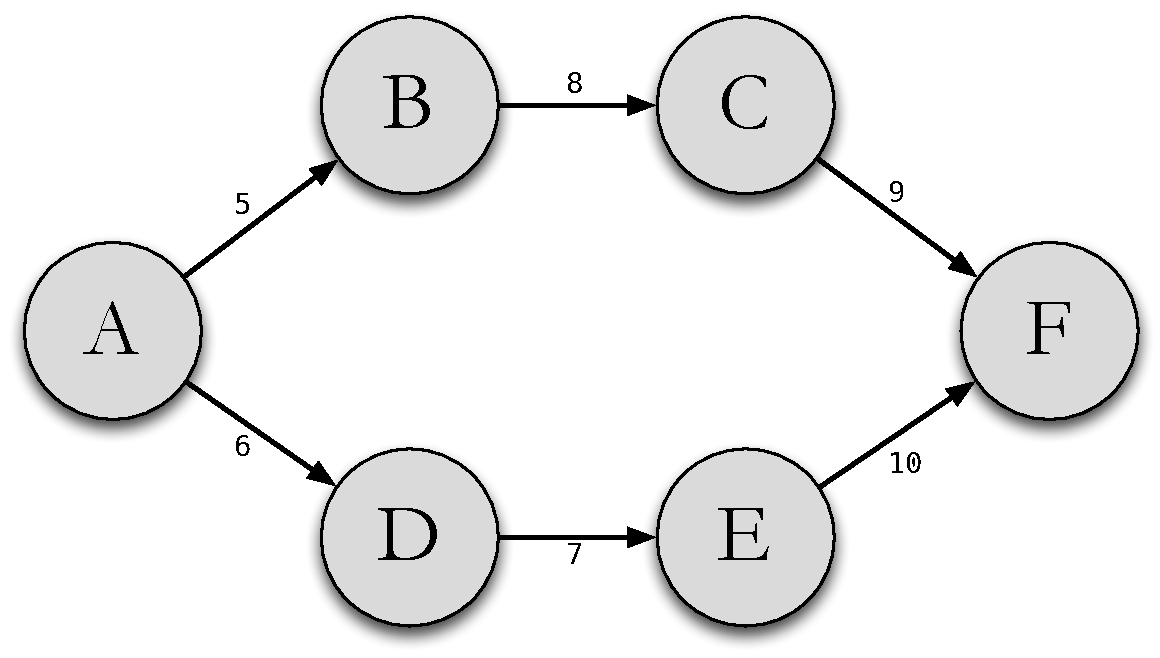
\includegraphics[width=0.5\textwidth]{examplegraph}
  \caption{An example directed graph with six vertices.}
  \label{fig:examplegraph}
\end{figure}

Let us establish some definitions.  We denote a \textbf{graph} as $G = \{\mathcal{V}, \mathcal{E}\}$ where $\mathcal{V}$ represents a unique set of \textbf{vertices}, and $\mathcal{E}$ a set of \textbf{edges}\cite{Koller:2009ty}.  We shall assume the set of vertices $\mathcal{V} = V_1, V_2, ..., V_n$.  A pair of vertices may be connected by an edge.  For the purposes of this dissertation, we shall require that all edges are \textbf{directed} (though for some applications outside this work, it is also possible for edges to be \textbf{undirected}).  Written as $V_i \rightarrow V_j$ (or equivalently $V_i \leftarrow V_j$ and $V_j \rightarrow V_i$), directed edges restrict graph traversal in one direction (thus enforcing a traversal order when reconstructing a region of the genome).  A vertex may have a number of incoming (outgoing) edges, the precise count being referred to as a vertex's \textbf{in- (out-) degree}.  We shall also refer to any vertex with an in-degree or out-degree greater than $1$ as a \textbf{junction}.

A \textbf{path} is a sequence of adjacent vertices that respects these edge relationships, i.e. $V_i, ..., V_k$ such that for every $j = i, ..., k$, we have $V_j \rightarrow V_{j+1}$.  In Figure \ref{fig:examplegraph}, the vertex sequence $A, B, C, F$ forms a path.  Similarly, a \textbf{trail} denotes a sequence of adjacent vertices, but does not respect the directionality of the edges.  In Figure \ref{fig:examplegraph}, the sequence $F, E, D, A$ forms a trail.  Edges can optionally carry \textbf{weight}, indicating an arbitrary cost for traversing from one vertex to another via particular edges.  Unless otherwise specified, we shall assume the edge weight is always $1$ (however, see Chapter \ref{ch:discussion} for a discussion on circumstances where weights might be a fruitful parameter in a graphical model of sequence assembly).

A \textbf{multi-color graph} is a useful extension for multi-sample scenarios.  Each edge carries additional metadata used to denote sample identity (e.g. each sample is assigned a unique "color").  All kmers in all samples are added to the graph, and following the edges with the same color yields the genome of that sample.  Many kmers will not be accessible when traversing paths or trails in one color versus another.  These motifs are the hallmark of most variation in a graphical setting.

Often in this dissertation, we will perform operations on a limited graph region wherein we process only vertices of interest and all edges present between them in the original graph.  This is referred to as an \textbf{induced subgraph} (which is \textit{not} technically synonymous with a subgraph, but for simplicity in this work, we will often drop the "induced" qualifier).  Let $\mathbf{V} \subset \mathcal{V}$.  The \textbf{subgraph} $G[\mathbf{V}] = \{\mathbf{V}, \mathcal{E'}\}$ where $\mathcal{E'}$ are all the edges $V_i \rightleftharpoons V_j \in \mathcal{E}$ such that $V_i, V_j \in \mathbf{V}$.

A \textbf{de Bruijn} graph represents fixed length symbols (vertices) and their overlaps (edges), with the added restriction that each symbol may only appear once in the graph\cite{Bruijn:1946va}.  Applied to assembly, each symbol is taken to be a genomic sequence of length $k$ (or \textbf{kmer}), with edges connecting vertices overlapping by $k-1$ bases\footnote{According to the original mathematical definition, a de Bruijn graph should represent \textit{every} possible symbol of length $k$, which makes the assembly formulation a subgraph rather than a graph.  However, none of the relevant literature refers to assembly graphs in this manner, so we shall carry on abusing the term.}.

To construct the initial graph, each sequenced read is broken up into $l-k+1$ kmers (where $l$ is the read length) and added to the graph as vertices, with edges being placed between adjacent kmers.  Overlapping reads should share kmers, and the adjacency information stored in the graph can be updated accordingly.  Thus processing one read at a time in this manner will yield a graph of overlaps for the entire dataset.

We rely on the Cortex assembly software for construction of the graph.  Cortex represents the graph on disk as fixed-width records (herein referred to as \textbf{CortexRecords}) consisting of a \textbf{CortexKmer} (defined as a odd-length kmer or its reverse complement, whichever is alphanumerically lower; two CortexKmers constructed from a forward sequence and the reverse complement of that sequence evaluate to the same object), coverage in each color, and a list of incoming and outgoing edges.  The edge lists utilize a minimalist description.  For incoming edges, only the first base of the preceeding kmer is stored; the rest of the kmer is assumed to be the $0$ to $k-1$ substring of the current kmer.  Likewise, for outgoing edges, the subsequent kmer is assumed to be the $1$ to $k$ substring of the current kmer plus the last base of the next kmer.  Figure \ref{fig:cortexrecords} lists three example records.  In the first record, the specified kmer has coverage $9$ in color $0$ (for our purposes, the child), $8$ in color $1$ (mother), and $5$ in color $2$ (father).  The trailing three columns encode edge information per color.  The first four characters of each column denote incoming edges to kmers with A, C, G, or T prefixes (or "." for no edge to that prefix).  The last four characters of each column denote outing edges to kmers with A, C, G, or T suffixes (or "." for no edge to that suffix).

\begin{figure}[h!]
  \centering
    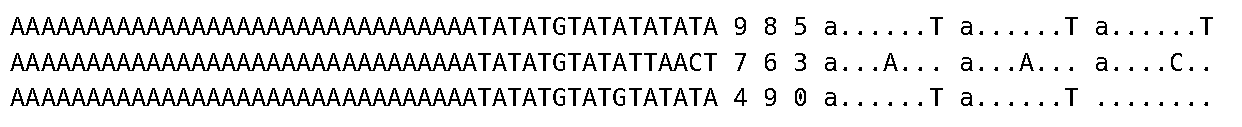
\includegraphics[width=\textwidth]{cortexrecords}
  \caption{Example CortexRecord entries.}
  \label{fig:cortexrecords}
\end{figure}

The Cortex de Bruijn graph can be easily represented as a hash table where each key is a CortexKmer and the associated value a list of incoming and outgoing edges.  This enables lookups to be performed in $\mathcal{O}(1)$ time, but requires the entire graph be loaded into memory.  While this makes sense from the perspective of a software developer writing assembly software (where one would assume that every kmer will be processed during the lifetime of the program's execution), it is cumbersome for our purposes.  DNMs are anticipated to be scant, which implies that the number of kmers that need to be examined is modest.  Furthermore, should we wish to scale to larger genomes in the future (e.g. mammalian genomes on the order of $3$ gigabases), we must be aware of the much greater difficulty in loading such a graph entirely into memory (unless one happens to be operating on a computer with several hundred gigabytes of available RAM).  Instead, we sort the Cortex graphs and perform a binary search whenever we need to load the CortexRecord associated with a particular CortexKmer.  This increases the time complexity for kmer lookups to $\mathcal{O}(\log{}n)$, but eliminates the need to load the entire graph to memory.

We define a series of utility functions that aid graph traversal.  The \textbf{\texttt{findRecord}} method retrieves the CortexRecord indexed by a kmer via a binary search over the sorted disk-based graph, or throws an error if the graph is not sorted.  The CortexKmer within the CortexRecord, in addition to carrying the text of the kmer, also stores a bit that indicates whether the stored orientation matches the requested orientation, which is useful for navigation.  The methods \textbf{\texttt{getPrevKmers}} and \textbf{\texttt{getNextKmers}} retrieve lists of kmers connected to incoming and outgoing edges of the specified kmer, orientation-matched to the kmer \texttt{sk}.

Many methods will accept two graphs rather than just one: a \textbf{clean} graph and a \textbf{dirty} graph.  The clean graph represents data where errors have been removed by the assembly software's automatic filtering process (coverage and contig length considerations).  The dirty graph represents data prior to this cleaning step.  When a kmer is absent from the clean graph or lacks incoming/outgoing edges, traversal can still continue if the dirty graph contains the requested kmer and edge information.  This overcomes an issue wherein \textit{overcleaned} data (data filtered with too stringent a threshold) causes erroneous gaps in the graph.  If carefully used, the dirty graph can be used to patch these holes without causing significant errors in the traversal.  Almost all methods with this double graph signature have a form that look like Algorithm \ref{alg:doublegraph}, wherein a single graph version of the same method is called, only to be called again if the operation on the clean graph was unsuccessful. 

\begin{algorithm}
\caption{Get next kmers from the clean graph, failing back to the dirty graph}
\label{alg:doublegraph}
\begin{algorithmic}[1]
\Function{getNextKmers}{clean, dirty, kmer, color}
    \State nextKmers = getNextKmers(clean, kmer, color)

    \If{(dirty != null \&\& nextKmers.isEmpty())}
        \State nextKmers = getNextKmers(dirty, kmer, color)
    \EndIf

    \State return nextKmers
\EndFunction
\end{algorithmic}
\end{algorithm}

Finally, we present in Figure \ref{fig:uml} the UML diagram of the relevant parts of codebase encapsulating the relationships between \texttt{CortexGraph} (manager of access to underlying disk representation of the multi-color de Bruijn graph); \texttt{CortexRecord} (decodes graph records into kmer, coverage, and incoming/outgoing edges); \texttt{CortexKmer} (the kmer itself, along with orientation information); the utility method object \texttt{CortexUtils} (a collection of miscellaneous methods written to facilitate graph navigation); and the \texttt{AnnotatedVertex} and \texttt{AnnotatedEdge} objects (used to store subgraphs and metadata).

\begin{figure}[h!]
  \centering
    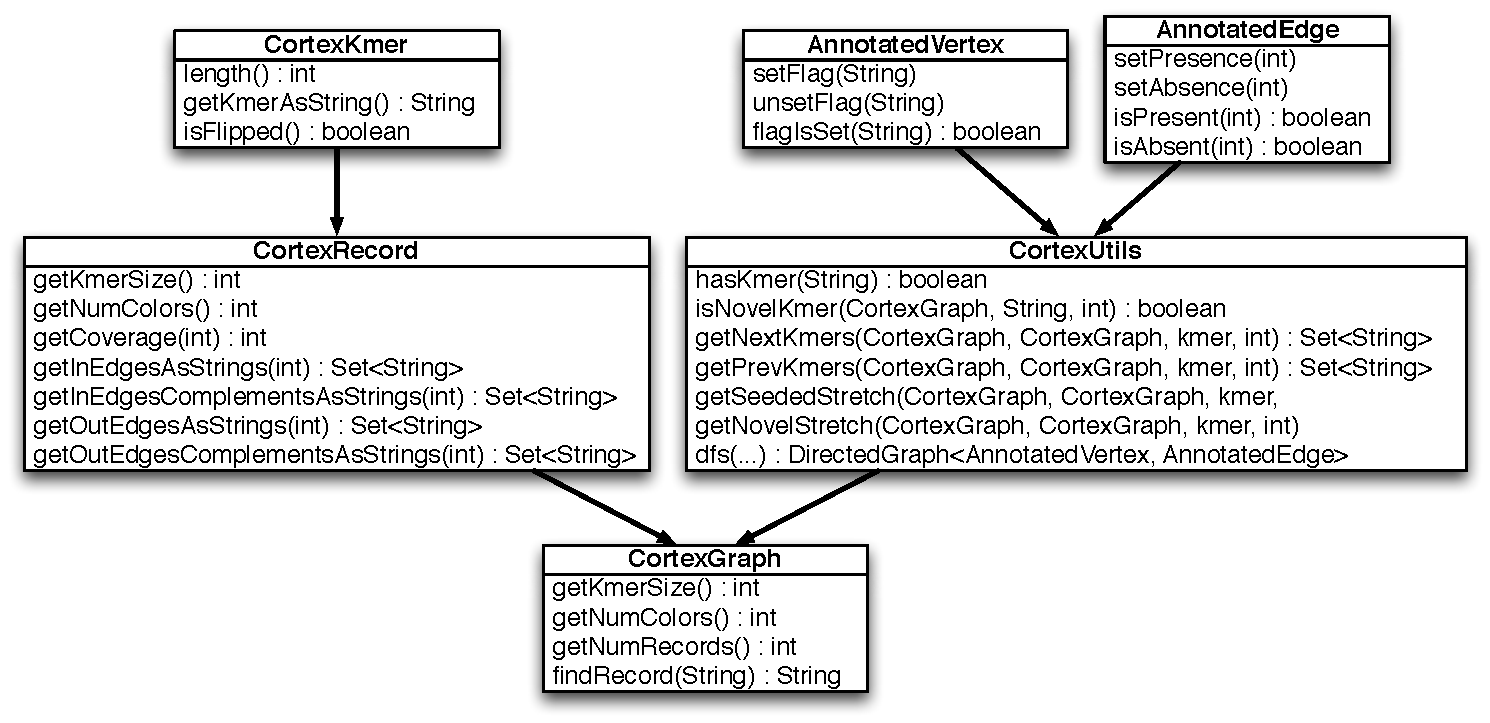
\includegraphics[width=\textwidth]{uml}
  \caption{Relationships between the \texttt{CortexGraph}, \texttt{CortexRecord}, \texttt{CortexKmer}, \texttt{CortexUtils}, \texttt{AnnotatedVertex}, and \texttt{AnnotatedEdge} objects.}
  \label{fig:uml}
\end{figure}

For clarity of the pseudocode presented below, we will refrain from referring to the object to which a method is bound.  For example, rather than specifying \texttt{CortexUtils.getNextKmer(...)} in an algorithm, we shall simply write \texttt{getNextKmer(...)}.  We \textit{will} refer to the parent object if doing so implies different data being accessed.  For example, \texttt{clean.findRecord(...)} and \texttt{dirty.findRecord(...)} refer to different data sources, the former being the error-cleaned data, the latter data that has not be processed in this manner.

\section{Variant motifs}
Just as reference-based methods search for motifs in the data representing variants (e.g. recurrent mismatches, gaps, or unusual truncations in the read alignments; read pairs aligning much further apart than expected; chimeras or inter-chromosomal alignments; etc.), so must we scan for indicative motifs in the assembly graph.  Before we discuss the precise nature of these motifs, it is useful to draw a distinction between "simple" and "complex" variants.  A "simple" variant is a SNP, insertion, or deletion that occurs within a single chromosome.  A "complex" variant could be a homologous or non-homologous recombination, translocation, or other interchromosomal exchange - something that does not fit within the confines of the straightforward SNP or indel classification.  The patterns inherent to these two categories of variants are very different.

\subsection{Simple variant motifs}
Simple variants in \textit{de novo} assembly data typically manifest as "bubbles" in the de Bruijn graph: regions where a variant has broken the homology between sequences, resulting in flanking kmers that are shared between the samples and spanning kmers that differ through the variant itself.  In a single diploid sample, this could be a heterozygous SNP or indel between two homologous chromosomes.  In a collection of haploid samples, one or more samples may differ from the others, resulting in the bubble.

As an illustration, consider three sequences from a mother-father-child pedigree, shown in Figure \ref{fig:db_graph_cartoon}a.  While the maternal and paternal haplotypes (green and blue, respectively) are identical, the child's haplotype (red) differs by a single C to G SNP.  Figure \ref{fig:db_graph_cartoon}b shows the resulting multi-color de Bruijn $k=3$ graph built from this data.  The mutation has given rise to the canonical bubble motif in the graph.  Three novel kmers (kmers present in the child and absent in the parents) spanning the variant allele are present.  Figure \ref{fig:snp_no_errors} is an equivalent graph for another simulated SNP, shown with more context and constructed with a much larger value of $k$ appropriate for $76$ - $100$ bp read lengths, typical of second-generation sequencing datasets (in this case, $k=47$).

\begin{figure}[h!]
  \centering
    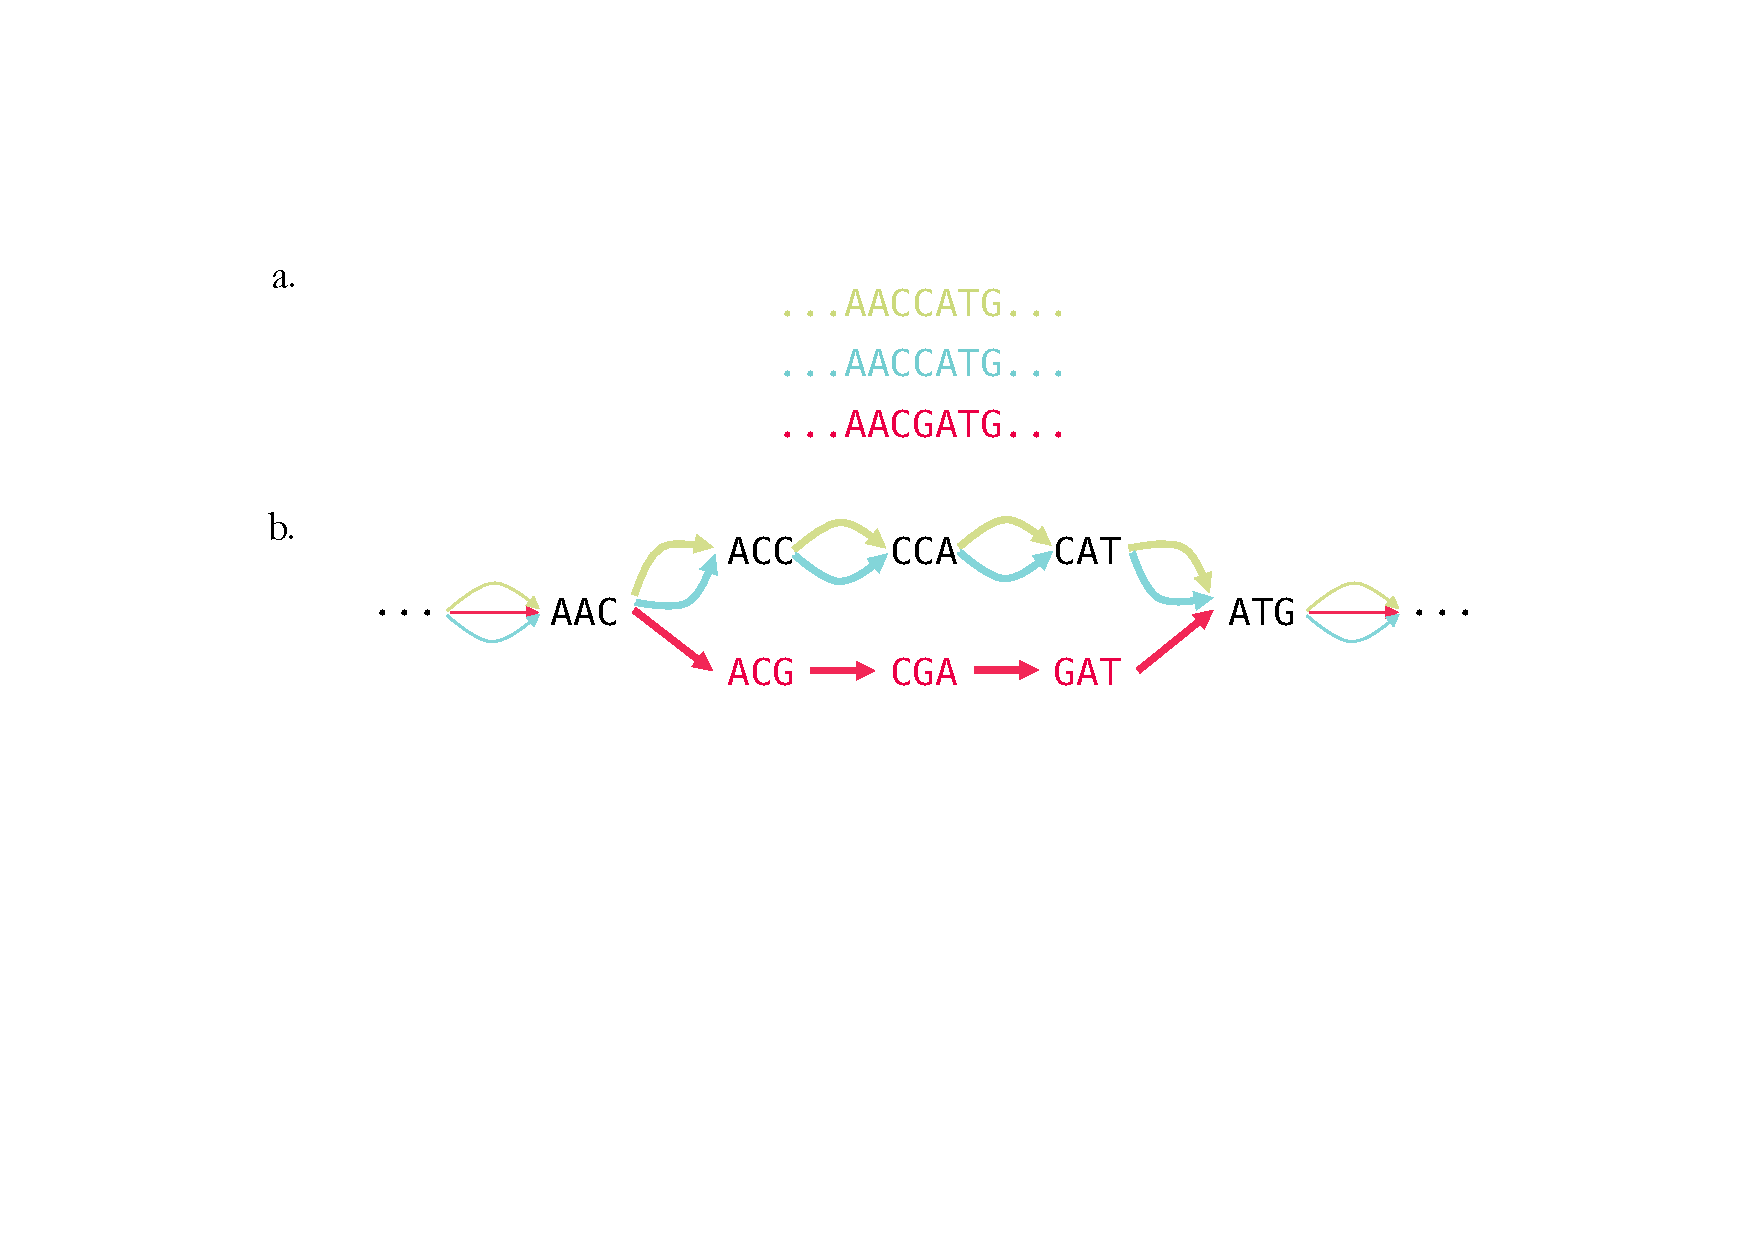
\includegraphics[width=\textwidth]{db_graph_cartoon}
  \caption{A simple variant motif for a C to G SNP.  a. Haploid sequences from a mother (green), father (blue), and child (red), the last differing from the first two by a single base substitution.  b. The resulting multi-color de Bruijn graph for $k=3$.  Red vertices denote kmers that are deemed "novel", i.e. present in the child and absent in the parents. Edge colors reflect the samples in which the connected pairs of kmers are found. Edges that are part of the bubble (variant call) are displayed with thicker lines.}
  \label{fig:db_graph_cartoon}
\end{figure}

\begin{figure}[h!]
  \centering
    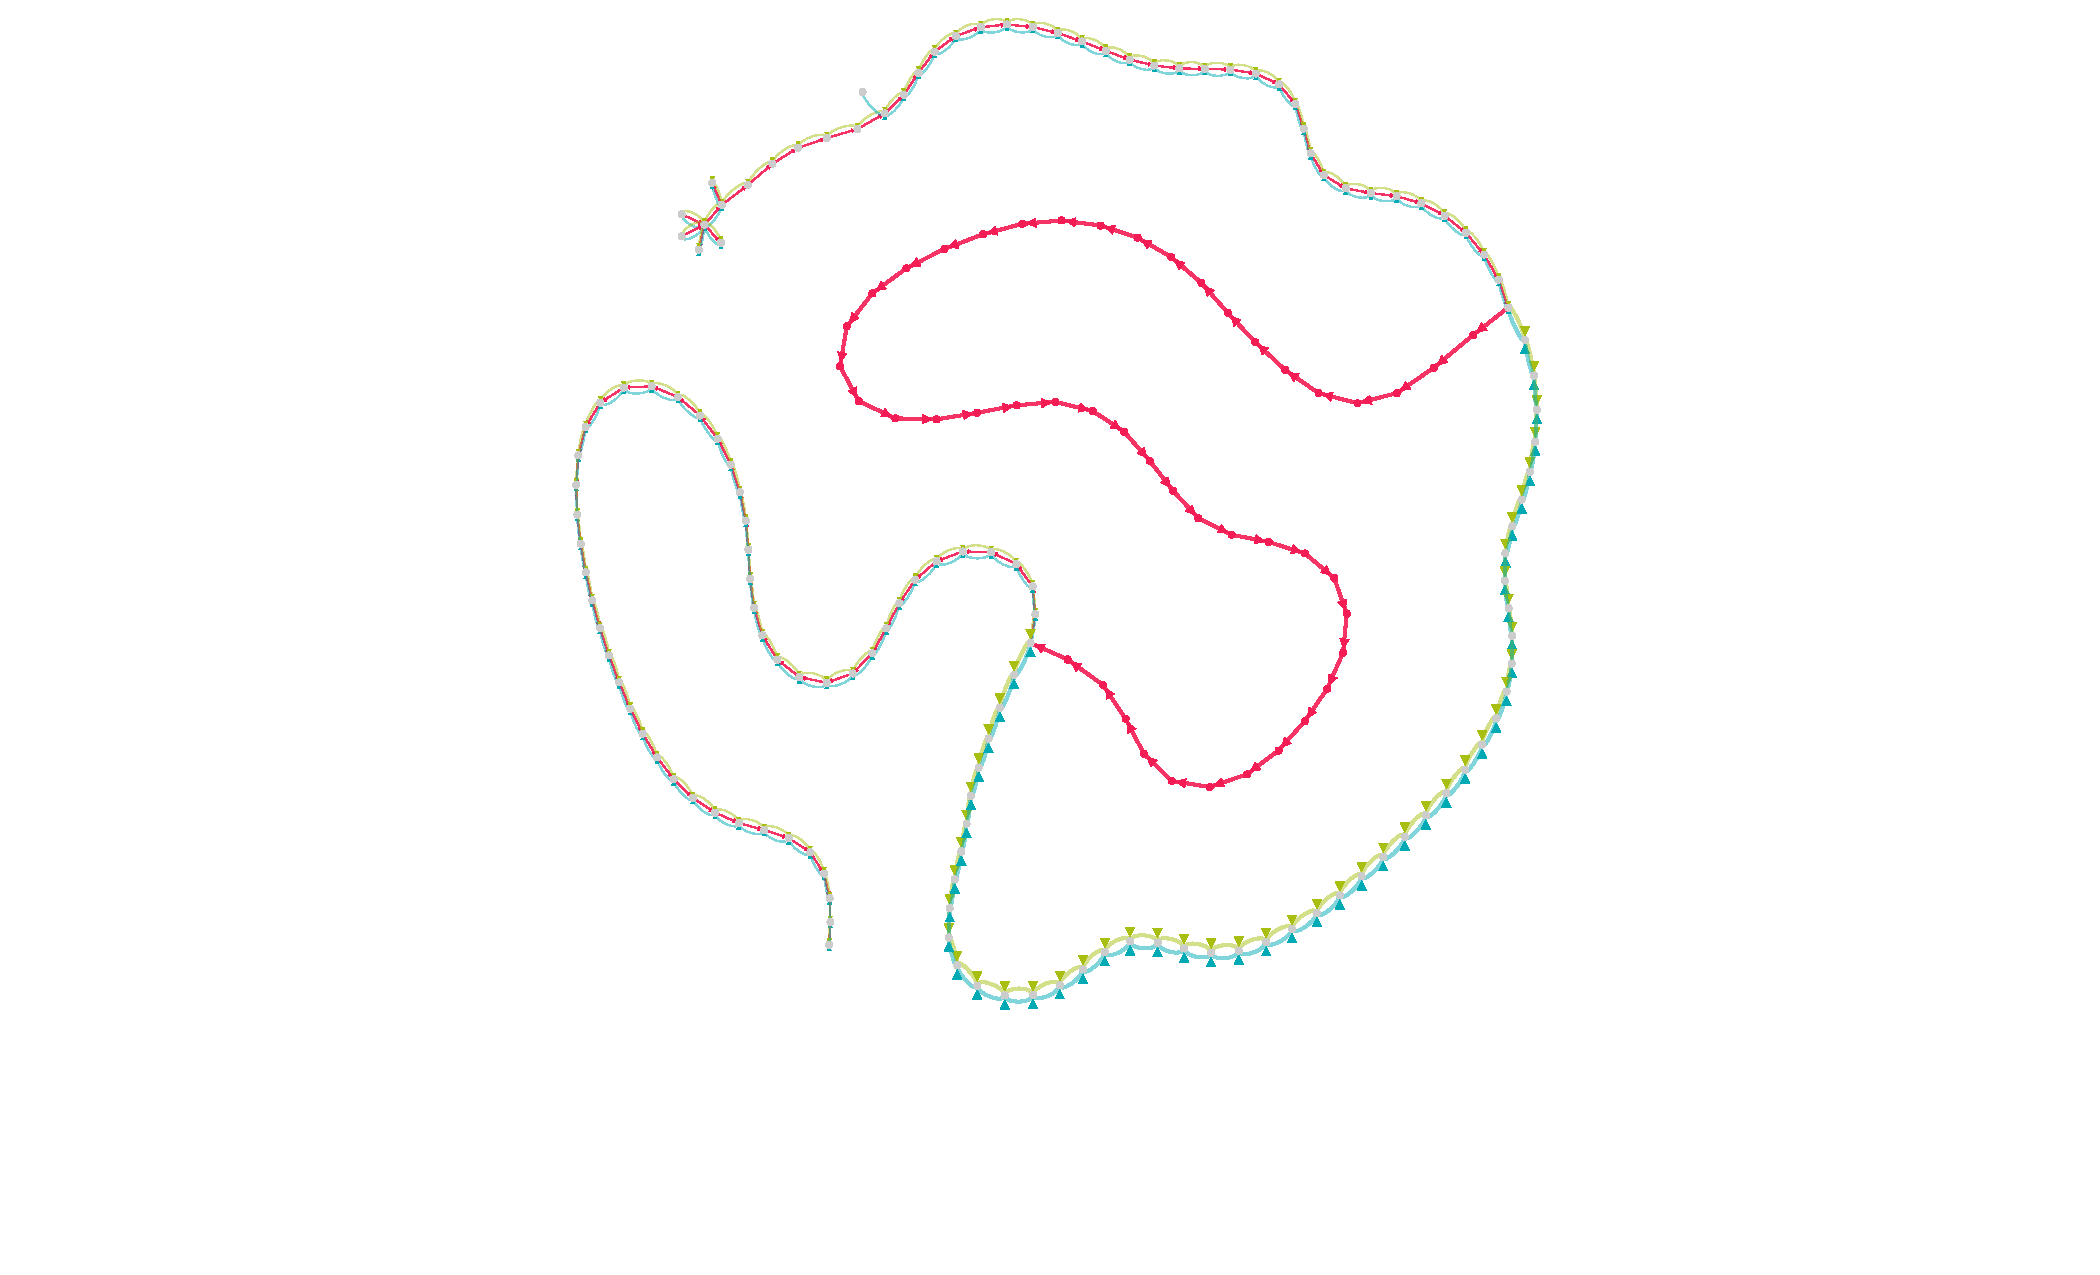
\includegraphics[width=0.5\textwidth]{snp_no_errors}
  \caption{A multi-color de Bruijn graph at $k=47$ for a haploid pedigree spanning a simulated \textit{de novo} SNP, produced by our VisualCortex software.  Vertex labels have been supressed for clarity.  Spatial layout is arbitrary and for display purposes only.}
  \label{fig:snp_no_errors}
\end{figure}

All simple variants will have this basic structure: a bubble in the graph that separates the variant samples from the non-variant samples.  The only major difference is the length of each branch: longer for an insertion in the child, shorter for a deletion (note that for short events, this is generally not apparent from the display, as evidenced by Figures \ref{fig:ins_no_errors} and \ref{fig:del_no_errors}).

\begin{figure}[h!]
  \centering
    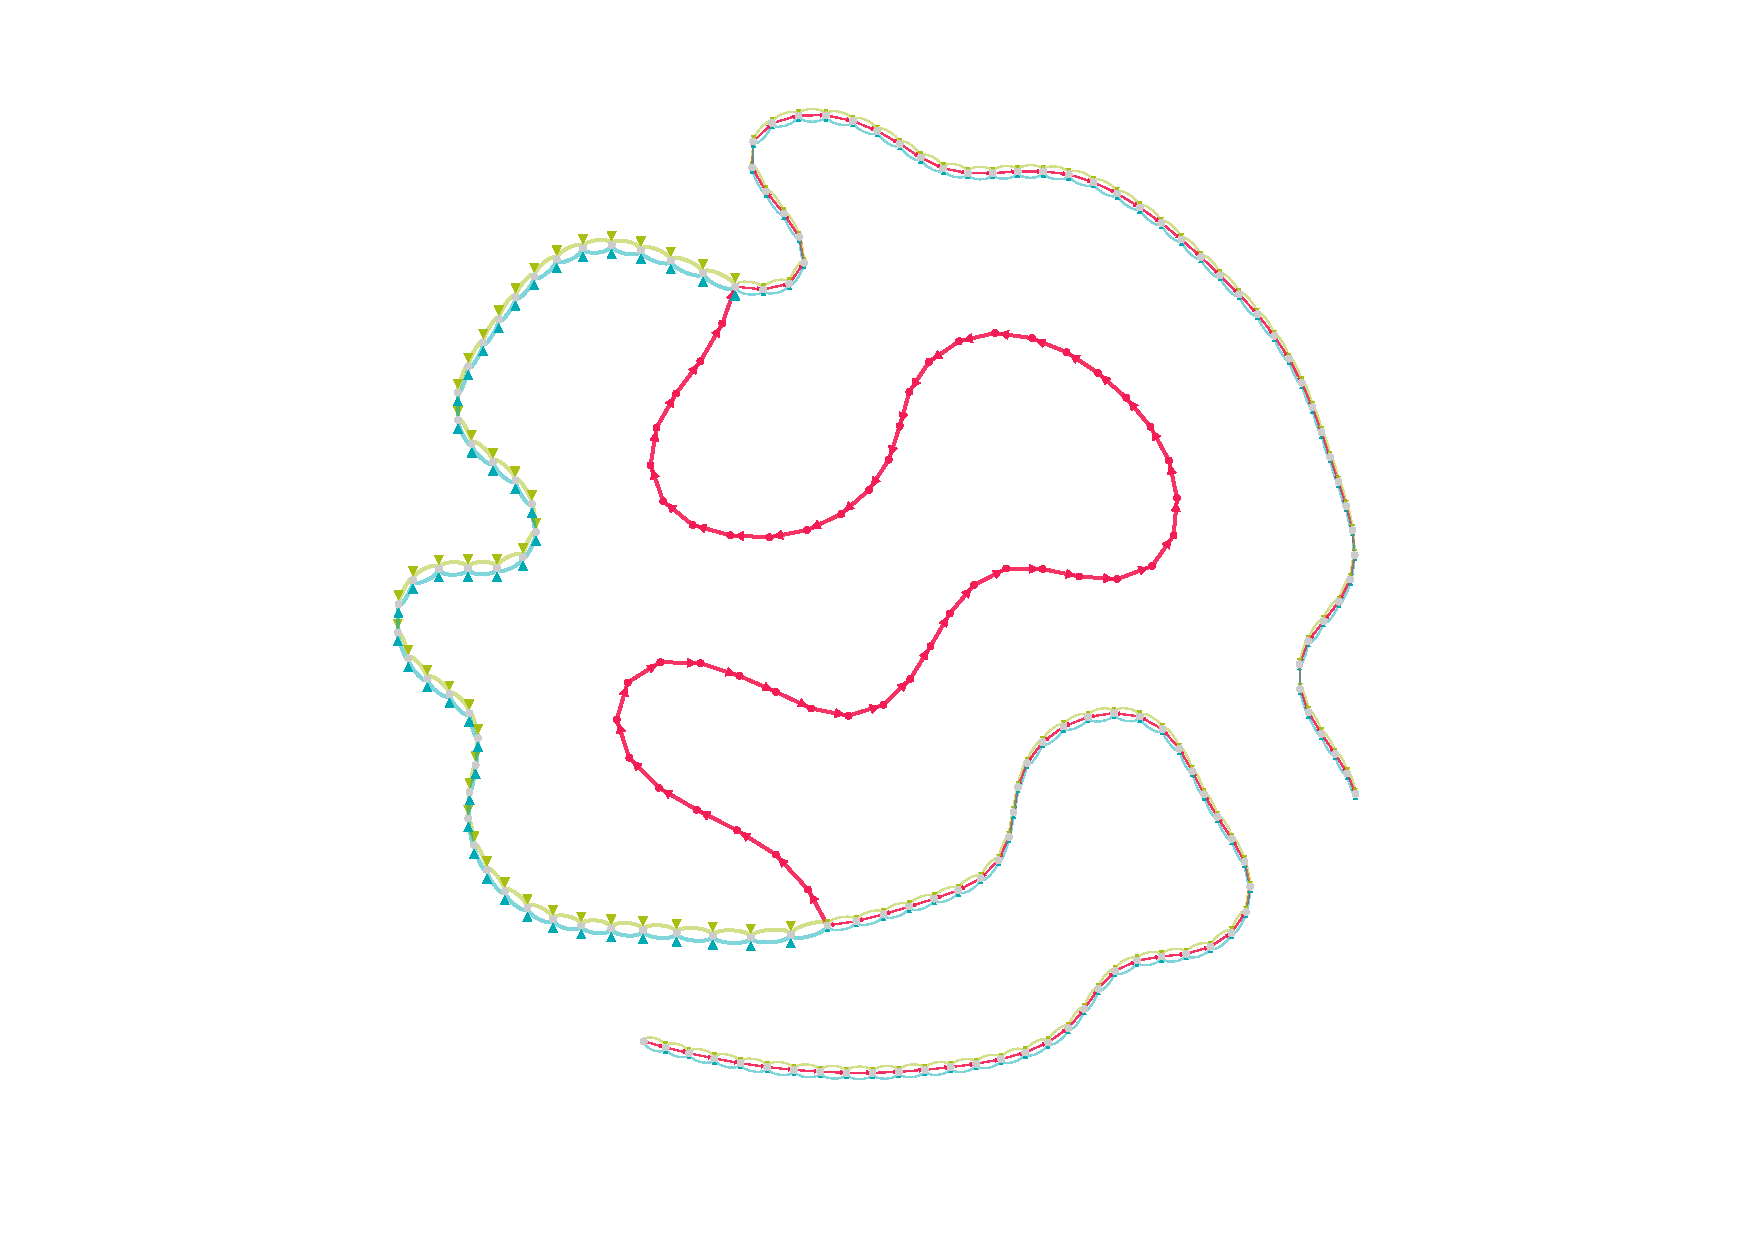
\includegraphics[width=0.9\textwidth]{ins_no_errors}
  \caption{A $5$ bp insertion in the child}
  \label{fig:ins_no_errors}
\end{figure}

\begin{figure}[h!]
  \centering
    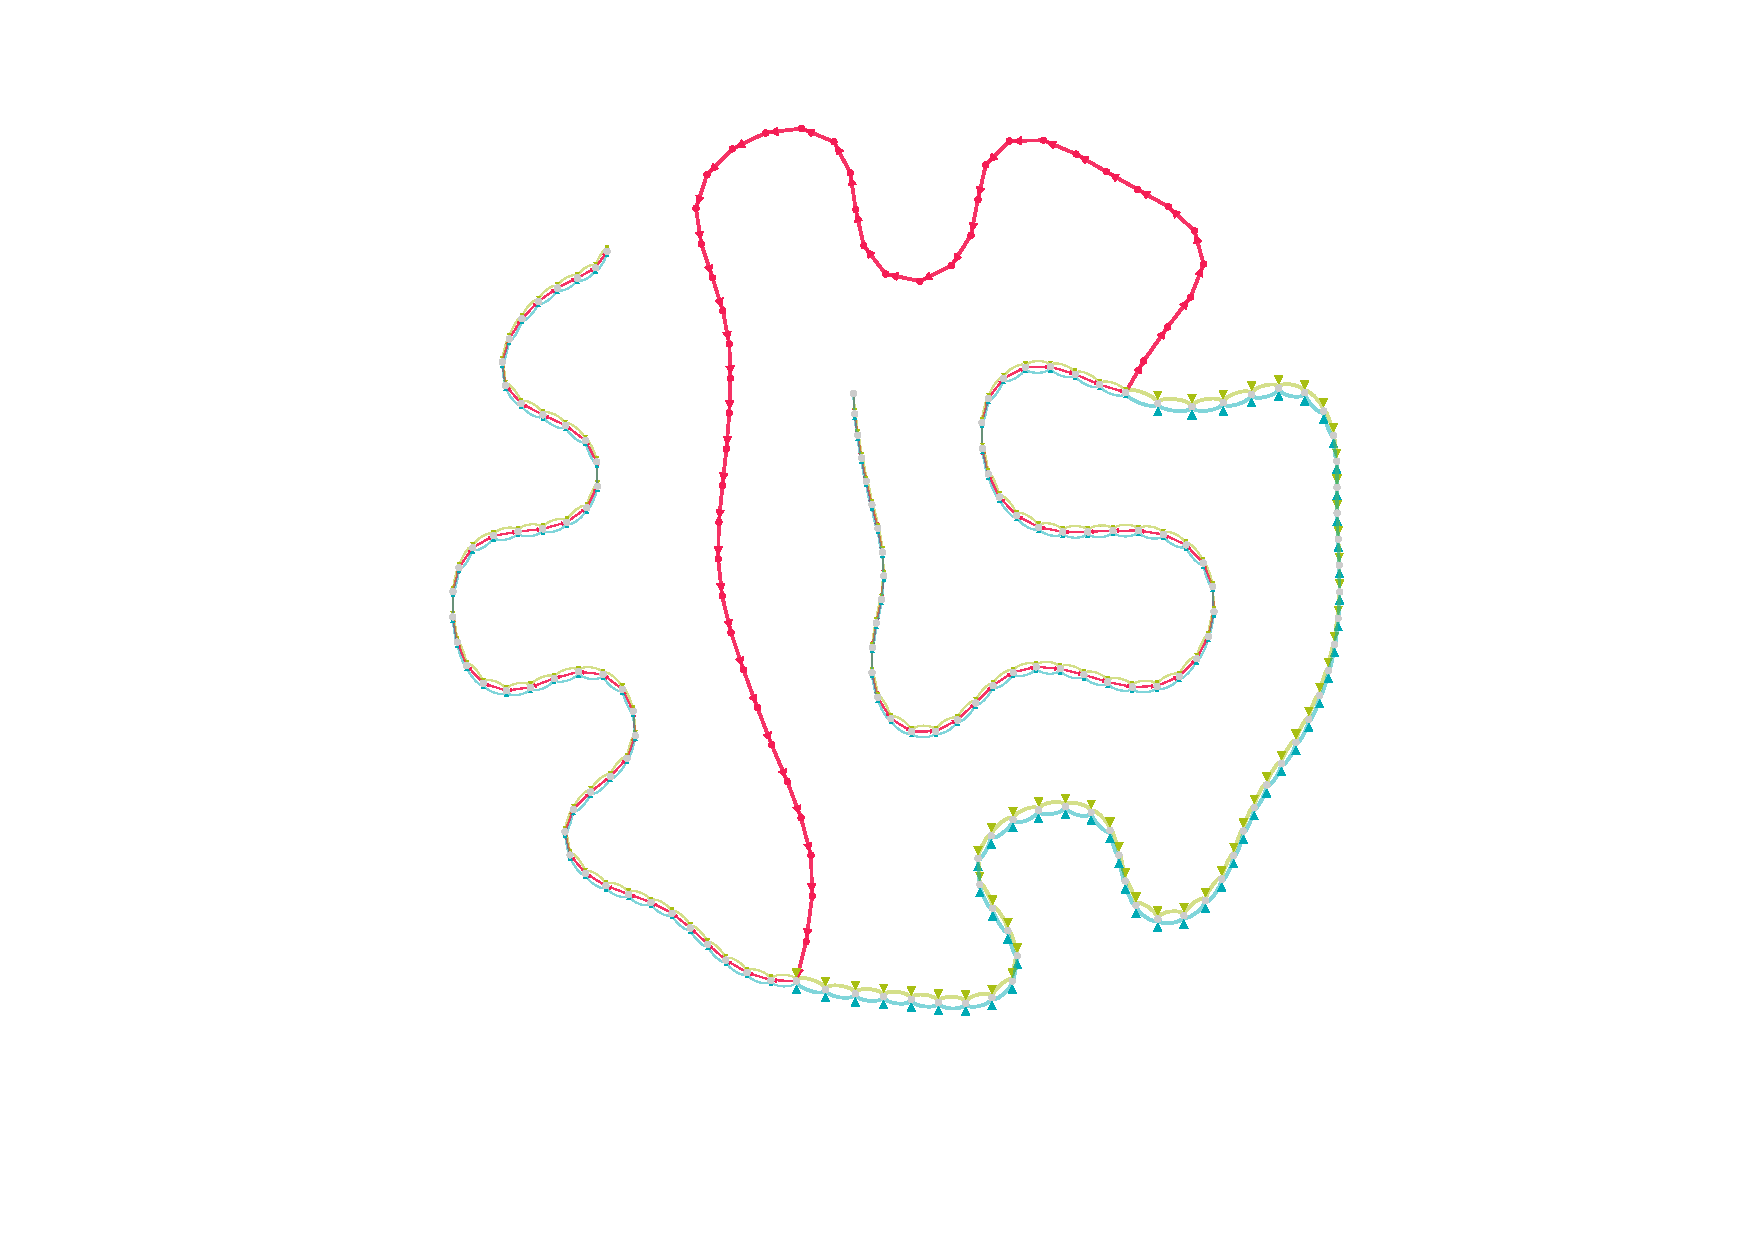
\includegraphics[width=0.9\textwidth]{del_no_errors}
  \caption{A $5$ bp deletion in the child}
  \label{fig:del_no_errors}
\end{figure}

Many variants may occur on the haplotypic background of one parent and not the other.  This is common in regions of the genome that are divergent between the two parents.  Figure \ref{fig:td_haplotypic_background} depicts one such simulated event.  A 41-bp tandem duplication has occurred on the background of the mother (evidenced by the presence of green edges), but not the father (thus the absence of blue edges).  In the flanking tails, edges shared between all three samples are present until a blue edge separates from the graph and connects to different vertices.  While not shown, these branches continue along the genome of the father.

\begin{figure}[h!]
  \centering
    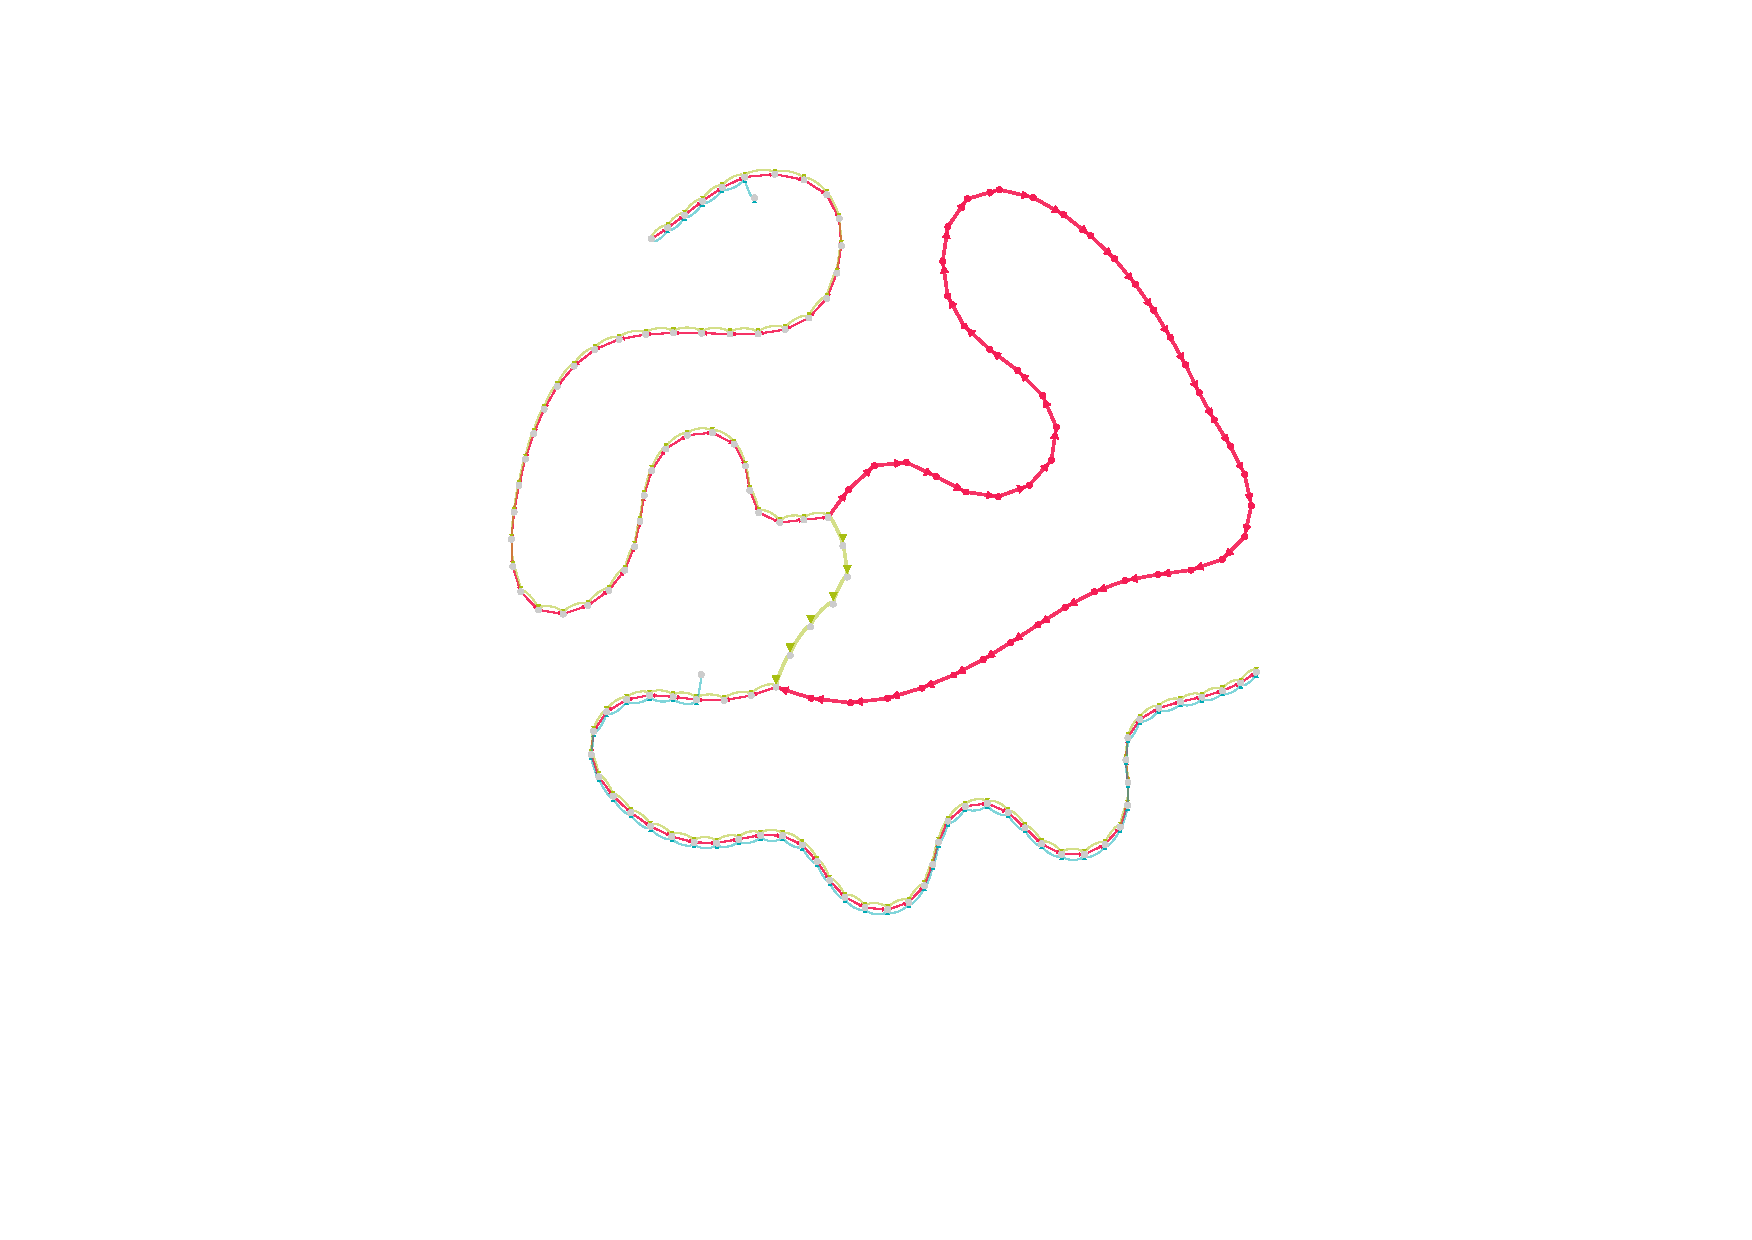
\includegraphics[width=0.9\textwidth]{td_haplotypic_background}
  \caption{A tandem duplication on the haplotypic background of the mother.}
  \label{fig:td_haplotypic_background}
\end{figure}

Finally, it is possible to encounter variants where the path through the graph taken by the child can appear to follow both the variant and non-variant paths, as demonstrated by Figure \ref{fig:inv_child_follows_parents}.  Such a scenario may arise by a mutation on a sequence with copy number greater than $1$: both the unaltered and altered sequences would then exist simultaneously in the child's genome.

\begin{figure}[h!]
  \centering
    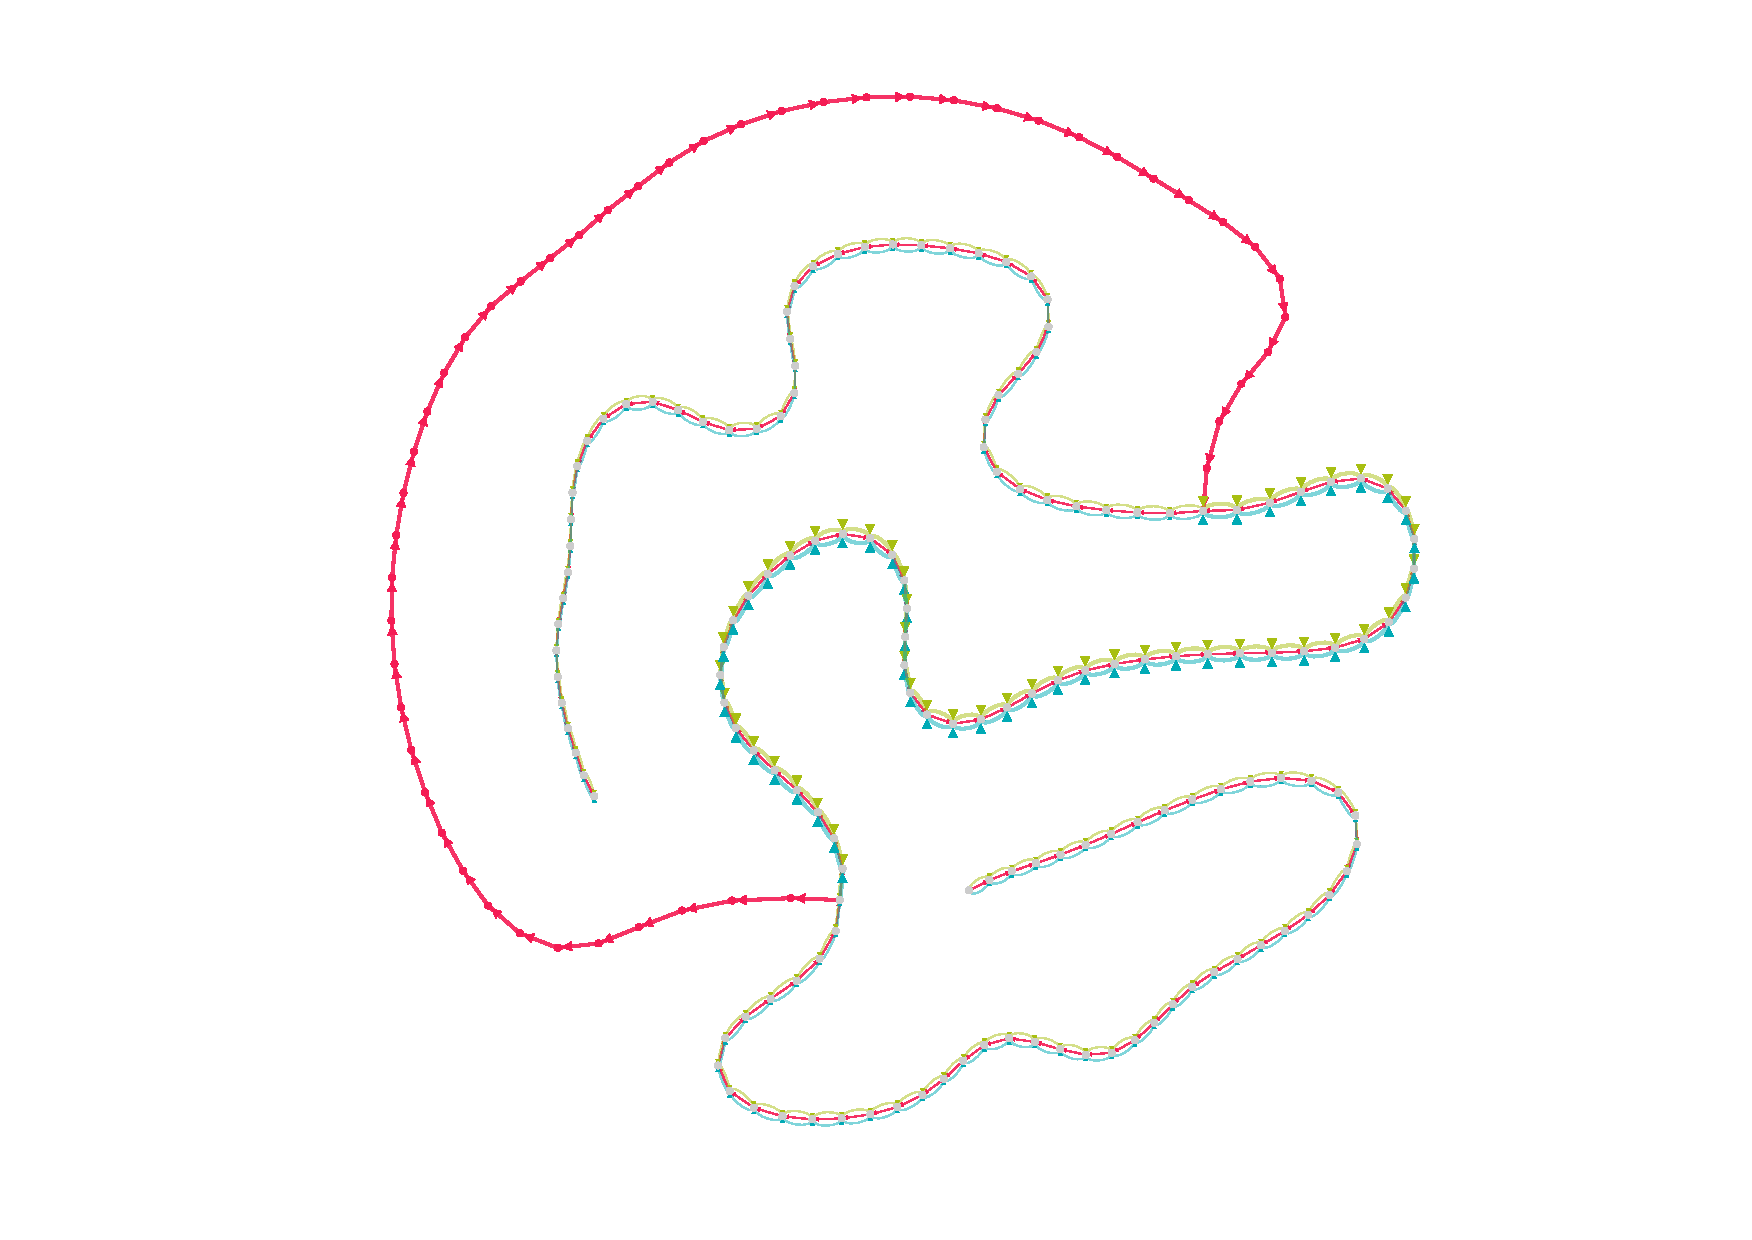
\includegraphics[width=0.9\textwidth]{inv_child_follows_parents}
  \caption{A variant wherein the child's path does not simply diverge from that of the parents, but rather navigates both.}
  \label{fig:inv_child_follows_parents}
\end{figure}

\subsection{Complex variant motifs}

\begin{figure}[h!]
  \centering
    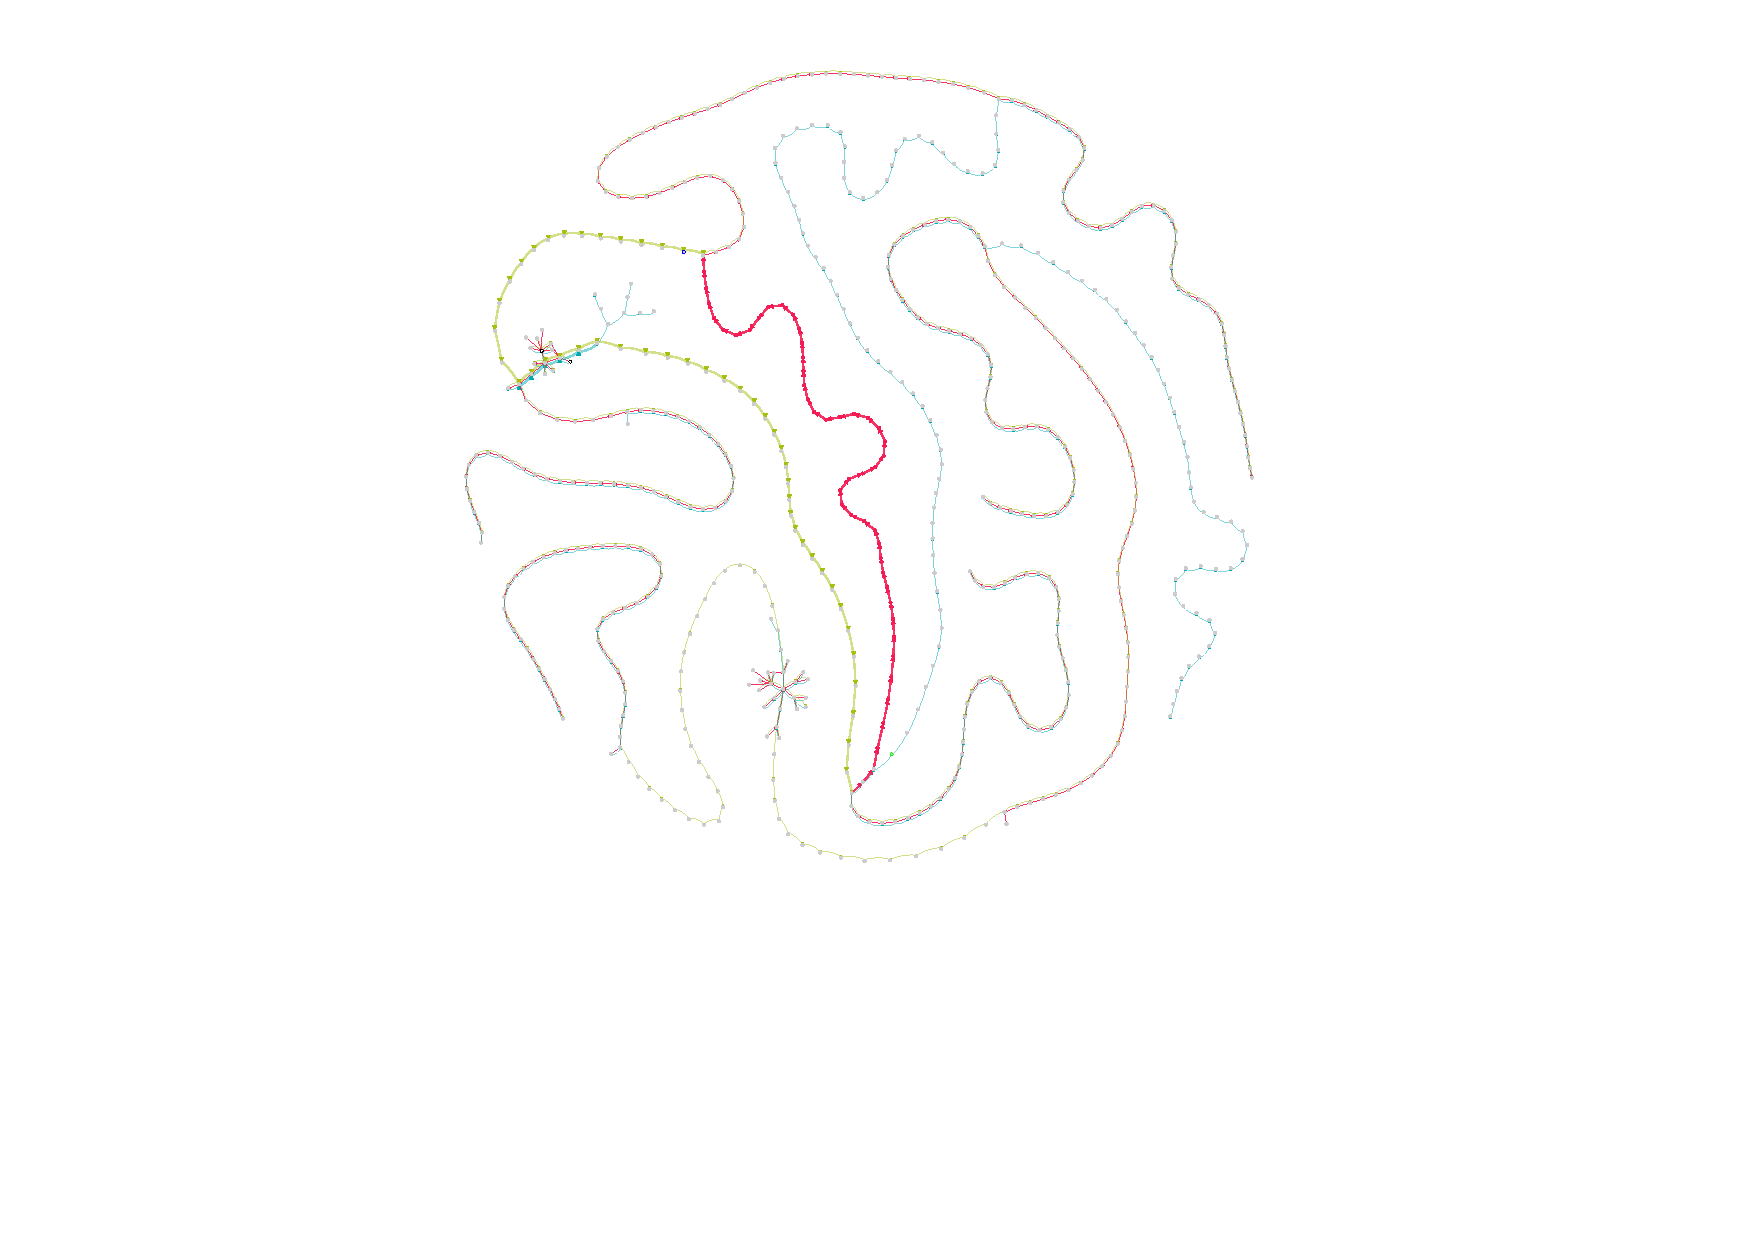
\includegraphics[width=0.9\textwidth]{gc}
  \caption{A gene conversion event}
  \label{fig:gc}
\end{figure}

Recombination events (allelic crossovers or gene conversion events; NAHR events) will not necessarily appear as bubbles.  Bubbles form in the graph when parental and progeny haplotypes diverge (at the site of a variant) and reconnect (at the flanking homologous regions).  In a recombination event, the haplotypes do not necessarily reconnect.  In a crossover or gene conversion event, as in Figure \ref{fig:gc}, the progeny's graph should follow one parent or the other, switching at the crossover site.  Gene conversions and other multiple crossovers may switch back and forth several times.  These events can be detected simply by keeping track of which parent's graph is apparently being followed.  However, we caution the reader that it's quite likely that many events of this nature will likely go uncalled or improperly called.  For such recombination events to be detected, a kmer spanning two proximal variants must be present.  This is unlikely to occur for simple crossovers, particularly in genomes of reasonably low heterozygosity, as neighboring variants beyond a kmer's length away will not give rise to novel kmers necessary for the event's detection.  It is perhaps slightly more likely for gene conversion events, where the multiple crossovers proximal to a variant exclusive to one of the parents will generate the sought-after novel kmer signal.

NAHR events are trickier; as these events are generally mitotic rather than meiotic events, the expected motif is that a child's graph should follow the same parent, but connect disjoint components of the graph (e.g. telomeres of different chromosomes) through novel kmers.  In principle, one should be able to detect such an event by testing whether removing the child's contribution to the pedigree subgraph results in disrupting the otherwise connected components\cite{Hopcroft:1971vx}.  In practice, however, NAHR events are mediated by homology between low-complexity regions of the subtelomeric genomic regions.  The homology will result in confounding connections between disparate regions of the graph.  An easier solution is to track the parent apparently being copied from and determine the chromosome of origin for each kmer present in the flanking regions of the novel kmers.  This is only feasible if one happens to have draft reference genomes for which a kmer's chromosome of origin can be approximately determined.

\subsection{Handling errors in sequencing}

\begin{figure}[h!]
  \centering
    \includegraphics[width=0.9\textwidth]{indel_with_errors_collapsed_and_expanded}
  \caption{Indel with sequencing errors in graph.  a. Selected extraneous branches expanded for illustrative purposes  b. All extraneous branches collapsed.}
  \label{fig:indel_with_errors_collapsed_and_expanded}
\end{figure}

Bubble and non-bubble motifs are trivial to find and navigate if there are no errors in the sequence data, but this situation rarely arises in real data.  Real data is subject to sequencing errors, making graph traversal much more difficult.  Errors manifest as extraneous branches in the graph, adding ambiguity to traversals.  Without a guide as to which branch to explore at a junction, we are either forced to abandon the traversal, make a guess, or explore all possible branches.  The first option is overly conservative; many variants will go untyped.  The second is hazardous; there is the very real potential for choosing erroneously and typing the variant incorrectly.  The last is computationally expensive; errors explode the complexity of the graph, making it prohibitively costly to find the correct path through the graph.

To solve this, recall that DNMs do more than open up a bubble motif in the graph.  Ideally, each kmer along the variant path is novel.  If we assume that branches following the novel branch at junctions are correct and linked with the current variant being explored, we can use these novel kmers as "sign posts" to mark successful traversals.  Navigating a branch and not seeing a sign post gives us adequate cause to abandon a branch in favor of another.

Figure \ref{fig:indel_with_errors_collapsed_and_expanded}a-b depict a simulated indel in imperfect data, the former with some of these extraneous branches displayed, the latter with them suppressed.  Branches with novel kmers (the red vertices) clearly complete the variant, while branches lacking these novel kmers are superfluous to the traversal and can be discarded without loss.  This limits the amount of unnecessary traversal in the graph, making it easier to find paths through the parental and child colors to form the variant.

\section{Calling and classifing \textit{de novo} variants}

Armed with an intuition as to how graphs behave in regions of \textit{de novo} variation, we can now describe the procedure for identifying and classifying a variant.  The overview involves five big steps (and associated substeps):

\begin{enumerate}
\item Identify confident and trusted novel kmers
\item Construct multi-color de Bruijn "trio" graphs (child, mother, father)
\item Load subgraph local to a novel kmer
\item Identify and classify variants in the subgraph
\item Evaluate performance
\end{enumerate}

We discuss these in details in the sections below.

\subsection{Identify confident and trusted novel kmers}

We first seek to build a list of novel kmers that are both \textit{confident} (i.e. unlikely to be sequencing errors) and \textit{trusted} (i.e. are unlikely to be the result of contamination).  Identification of the novel kmers themselves is trivial; we simply build a list of kmers that appear in the child but are completely absent in the parents.  The subsequent filtering steps are described below.

\subsubsection{Remove low coverage kmers}

For a deeply sequenced sample, we expect all kmers in the genome to be of similarly high coverage.  While there will inevitably be regions of the genome where coverage is poor owing to failure to amplify regions with high GC content, the Lander-Waterman statistics in Chapter \ref{ch:motivation} suggest we should easily see many copies of the entire \textit{P. falciparum} genome at a coverage of $100x$.  We can therefore assume that failure to reach a certain coverage threshold is indicative of sequencing error, and such kmers can be removed as candidates from the novel kmer list.

The problem remains as to where the threshold should be set.  For each sample, we plotted the histogram of kmer coverage, shown in Figure \ref{fig:covthreshold}, smoothing the resulting distribution with a non-parametric LOESS fit.  The smoothed histogram makes it easier to find the first local minimum using Algorithm \ref{alg:localminimum}.

\begin{algorithm}
\caption{Compute the local minimum of a kmer coverage distribution}
\label{alg:localminimum}
\begin{algorithmic}[1]
\Function{firstLocalMinimum}{coverageHist}
    \State y = laggedDifferences(c(INT\_MAX, x)) > 0L
    \State y = cumSum(equalRunLengths(y).lengths)
    \State y = y[seq(2L, length(y), 2L)]

    \State return(y[2])
\EndFunction
\end{algorithmic}
\end{algorithm}

\begin{figure}[h!]
  \centering
    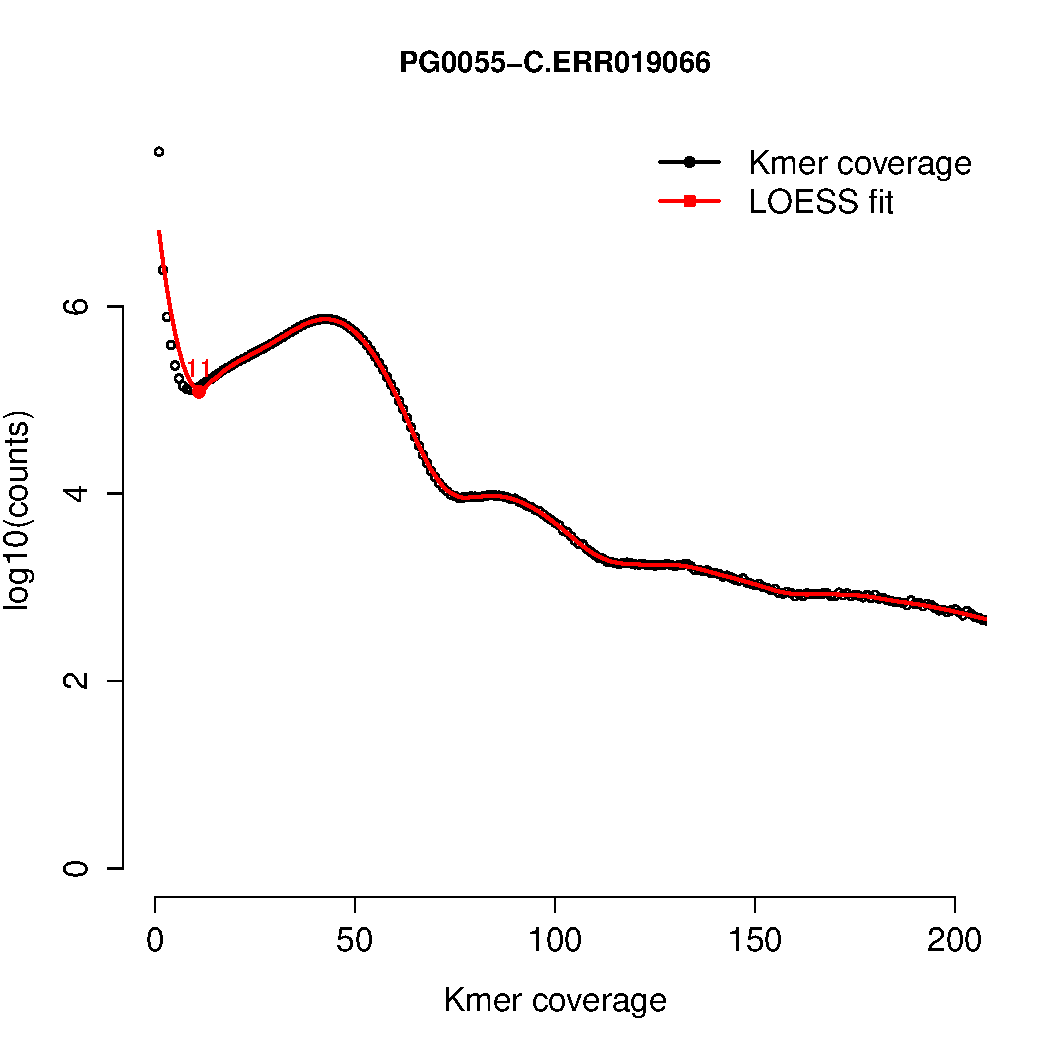
\includegraphics[width=0.9\textwidth]{covthreshold}
  \caption{Kmer coverage histogram for a real sample, with LOESS fit}
  \label{fig:covthreshold}
\end{figure}

\subsubsection{Remove possible contaminants}

Contamination can occur during sequencing library preparation due to handling from human operators (transferring either bacterial or human genetic material to the library) or from other samples (often from different species) being processed in the same laboratory.  Contamination would result in kmers that appear novel - owing to their absense in the parents - but are irrelevant for our study.  It is perhaps not a paramount concern when processing \textit{P. falciparum} data, as the genome is very different than any other sample likely to be a contaminant.  However, it may contribute false-positives that we can easily mitigate.

To remove the effects of contamination, we run every confident novel kmer through BLAST\cite{Altschul:1990dw}.  Specifically, we used the \texttt{blastn} package and all available BLAST nucleotide databases to identify the likely species of every confident novel $47$-mer in each sample.  Any unidentified kmer or apparently \textit{P. falciparum} kmer was retained; all others were removed.  In practice, this removes anywhere from dozens to thousands of kmers from needing to be considered; as evidenced by Figure \ref{fig:contam}, the exact number varies as each sample is prepared independently, at different times and by different personnel.

\begin{sidewaysfigure}[h!]
  \centering
    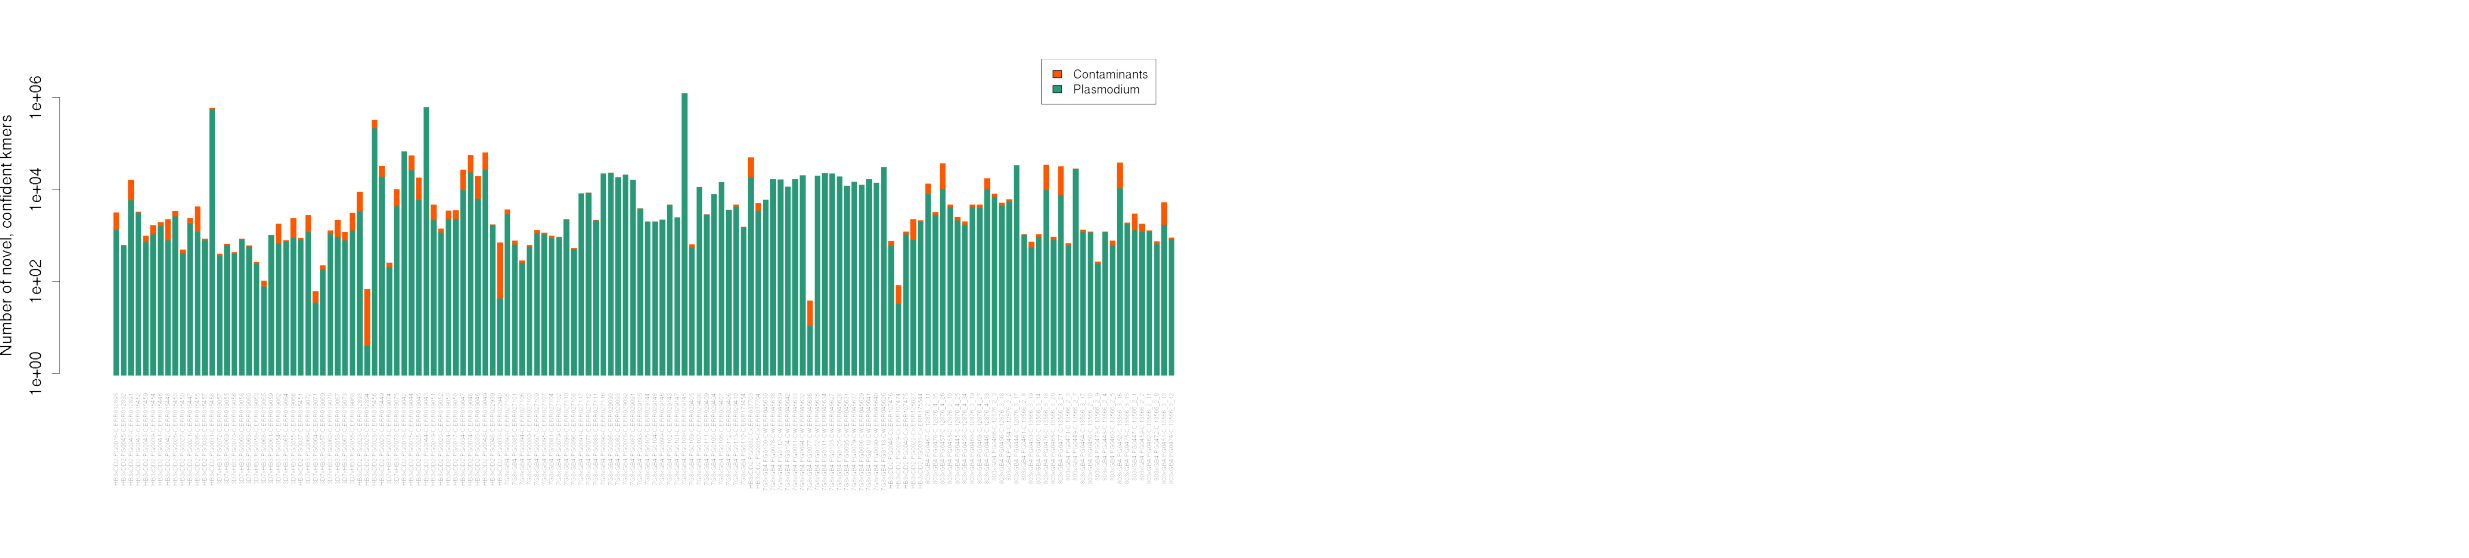
\includegraphics[width=\textwidth]{contam}
  \caption{Removal of contaminating kmers; \textit{P. falciparum} kmers are shown in green; the putative contaminants are shown in orange.}
  \label{fig:contam}
\end{sidewaysfigure}

\subsection{Construct multi-color de Bruijn "trio" graphs}

To construct the "trio" graphs, we perform assembly on each sample with the \textit{Cortex} \textit{de novo} assembly software\cite{Iqbal:2012fx} following the recommended workflow\cite{Turner:2015ve}.  Briefly, each sample is assembled using the \texttt{build} command at a kmer size of $47$ bp\footnote{This setting results from evaluations on optimal kmer size for maximizing contig length, despite not needing to produce contigs for our analyses} and ignoring nucleotides with an Illumina quality score less than $5$.  Each sample was then cleaned of likely sequencing errors with the \texttt{clean} command using automatically calculated coverage and supernode (unambiguous runs of kmers with in/out degree of $1$) length thresholds.  Finally, the graph for the child was merged into a \textit{clean} trio graph, and separately, a \textit{dirty} trio graph (one using the uncleaned graph data) using the \texttt{join} command.  This multi-color graph consists of child, mother, and father.  For our purposes with \textit{P. falciparum}, "child" is assigned color $0$, "mother" (the first parent of the cross) to color $1$, and "father" to color $2$.  Read threading was \textit{not} applied, as in our analyses, there is no need for contigs, just the graph data structure.

\subsection{Load subgraph local to a novel kmer}

To facilitate variant calling, we must process regions of the graph likely to harbor DNMs.  While it is technically possible to load a \textit{P. falciparum} graph into RAM (owing to its small $23$ megabase genome), it is unlikely such a solution would scale to larger genomes.  It is also cumbersome to do so when there are only on the order of dozens, perhaps hundreds, of variants to be discovered per genome.  Therefore, we adopted a solution of fetching only relevant parts of the genome as necessary, operating on the local subgraph surrounding the putative variant, rather than on the entire graph at once.

\subsubsection{Depth-first search}

Graph exploration is an \textit{online} problem, meaning the structure of the graph cannot be known until it is explored.  As a non-linear data structure, it is not trivial to determine where to start and stop exploring a graph.  During traversal, one may encounter junctions (due to errors or homology) without any additional information as to which branch to choose.  Graphs sometimes loop back onto themselves, necessitating that we keep track of our walk so that we do not end up traversing endlessly in circles.  Incorrect decisions in the traversal cannot always be detected, requiring appropriate stopping conditions to abort a traversal if no fruitful data is discovered.

Typically, graph exploration can be accomplished with a so-called \textit{depth-first search}, or DFS.  The basic premise of a DFS is summarized in Algorithm \ref{alg:dfs}: start at a vertex, walk in a chosen direction until a junction is encountered, choose one branch and repeat the DFS from that point until it is deemed appropriate to stop, then jump back to the junction to choose the next branch, and repeat until completion.  In practice, this approach has some drawbacks that manifest quickly in real data.  First, the basic DFS algorithm terminates only when there are no more vertices left to traverse, which is overkill for our purposes.  Second, all branches are treated equally.  For our purposes, branches containing errors are not important and should be discarded lest they confuse later algorithms trying to find paths through bubbles in order to type variants.  Third, this requires us to explore three graphs separately, which is inefficient.

\begin{algorithm}
\caption{A basic, iterative depth-first search}
\label{alg:dfs}
\begin{algorithmic}[1]
\Function{idfs}{graph, vertex}
  \State $s = \textrm{new Stack()}$
  \State $\textrm{visited} = \{\}$
  \State $\textrm{s.push(vertex)}$

  \While{\textrm{!s.isEmpty()}}
    \State $current = s.pop()$
    \If{($\textrm{visited.contains(current)}$)}
        \State $\textrm{next}$
    \EndIf
    \State $\textrm{visited.add(current)}$

    \For{$\textrm{v in graph.nextVertices(vertex)}$}
        \State $\textrm{s.push(v)}$
    \EndFor
  \EndWhile
\EndFunction
\end{algorithmic}
\end{algorithm}

The solution is to instead conduct a DFS with stopping conditions and recursively.  Stopping conditions, specifying the conditions upon which a traversal is deemed "successful" or "failed" allow us to decide certain branches in the subgraph are unfruitful for analysis.  The recursive traversal allows us to act on the result of the stopping condition, adding it to the subgraph if successful, discarding it if not.  This is described in Algorithm \ref{alg:rdfs}.

\begin{algorithm}
\caption{The recursive depth-first search with arbitrary stopping conditions}
\label{alg:rdfs}
\begin{algorithmic}[1]
\Function{rdfs}{clean, dirty, kmer, color, g, stopper, depth, goForward, history}
    \State firstKmer = kmer

    \State sourceKmersAllColors = goForward ? getPrevKmers(clean, dirty, kmer) : getNextKmers(clean, dirty, kmer)
    \State sourceKmers = sourceKmersAllColors.get(color)

    \State dfs = new AnnotatedGraph()

    \Repeat
        \State cv = kmer

        \State cr = clean.findRecord(cv)
        \If{(cr == null \&\& dirty != null)}
            \State cr = dirty.findRecord(cv)
        \EndIf

        \State prevKmers = getPrevKmers(clean, dirty, cv)
        \State nextKmers = getNextKmers(clean, dirty, cv)
        \State adjKmers  = goForward ? nextKmers : prevKmers

        \State addVertexAndConnect(dfs, cv, prevKmers, nextKmers)

        \If{(stopper.keepGoing(cr, g, depth, dfs.vertexSet().size(), adjKmers.get(color).size()) \&\& !history.contains(kmer))}
            \State history.add(kmer)

            \If{(adjKmers.get(color).size() == 1)}
                \State kmer = next(adjKmers.get(color))
            \ElsIf{(adjKmers.get(color).size() != 1)}
                \State childrenWereSuccessful = false

                \For{(ak in adjKmers.get(color))}
                    \State branch = dfs(clean, dirty, ak, color, g, stopperClass, depth + isNovelKmer(cr) ? 0 : 1, goForward, history)

                    \If{(branch != null)}
                        \State addGraph(dfs, branch)
                        \State childrenWereSuccessful = true
                    \EndIf
                \EndFor

                \If{(childrenWereSuccessful || stopper.hasTraversalSucceeded(cr, g, depth, dfs.vertexSet().size(), 0))}
                    \State return dfs
                \EndIf
            \EndIf
        \ElsIf{(stopper.traversalSucceeded())}
            \State return dfs
        \Else
            \State return null
        \EndIf
    \Until{(adjKmers.get(color).size() == 1)}

    \State return null
\EndFunction
\end{algorithmic}
\end{algorithm}

Stopping conditions are implemented as a callback object, permitting programmer-specified limits for different situations.  To type DNMs, we begin traversal at a novel kmer, walking forward and backward in the graph until the stopping conditions are met.  We then explore the parental graphs based on the subgraph we loaded for the child.  As the parental traversals have some additional information (namely, the presence of the child's subgraph allows us to check if a parental traversal has diverged and rejoined from the graph), the stopping conditions are different.

The stopping condition callback object implements two boolean methods: \texttt{hasTraversalSucceeded} and \texttt{hasTraversalFailed}.  Both of them may return \texttt{false}, in which case the traversal continues.  If either returns \texttt{true}, traversal is halted and the branch is evaluated for retention or rejection.

\subsubsection{Stopping conditions for child}

The child's stopping conditions on traversal success or failure are provided in Algorithm \ref{alg:child_hasTraversalSucceded} and \ref{alg:child_hasTraversalFailed}, respectively.  For the child, success is approximately determined by having explored a novel kmer stretch in the graph to the point that it has rejoined the parental graphs.  However, we purposefully continue reading another $50$ kmers before returning success.  If more novel kmers are recovered in that span, we reset our counters and continue walking.  This facilitates two things: the absence of novel kmers due to sequencing errors or overthresholding, and typing complex variants that may have short stretches of non-novel kmers.  Failure is determined by a number of criteria, including the absence of novel kmers, low complexity regions, having no more branches to explore, having reached a maximum graph depth, or having reached a maximum graph size.

\begin{algorithm}
\caption{Child's traversal success determination method}
\label{alg:child_hasTraversalSucceded}
\begin{algorithmic}[1]
\Function{hasTraversalSucceeded}{cr, g, depth, size, edges}
    \If{(goalSize == 0 \&\& (cr.getCoverage(1) > 0 || cr.getCoverage(2) > 0))}
        \State goalSize = size
        \State goalDepth = depth
    \EndIf

    \If{(goalSize > 0 \&\& isNovel(cr))}
        \State goalSize = size
        \State goalDepth = depth
    \EndIf

    \State return (goalSize > 0 \&\& (size >= goalSize + 50 || isLowComplexity(cr) || edges == 0))
\EndFunction
\end{algorithmic}
\end{algorithm}

\begin{algorithm}
\caption{Child's traversal failure determination method}
\label{alg:child_hasTraversalFailed}
\begin{algorithmic}[1]
\Function{hasTraversalFailed}{cr, g, depth, size, edges}
    \State return !isNovel(cr) \&\& (isLowComplexity(cr) || edges == 0 || depth >= 5 || size > 5000)
\EndFunction
\end{algorithmic}
\end{algorithm}

\subsubsection{Stopping conditions for parents}

The parents' stopping conditions on traversal success or failure are provided in Algorithm \ref{alg:parent_hasTraversalSucceded} and \ref{alg:parent_hasTraversalFailed}, respectively.  Success is determined by having diverged from the child's graph and rejoined it.  Care is taken to ensure that we have rejoined the graph at a boundary of the novel kmer stretch, rather than some ther part of the graph obtained when trying to read some extra flanking data in Algorithm \ref{alg:child_hasTraversalSucceded}.  Failure is determined by a number of criteria, including having reached a maximum graph size, having reached a maximum graph depth, or low complexity regions.

\begin{algorithm}
\caption{Parents' traversal success determination method}
\label{alg:parent_hasTraversalSucceded}
\begin{algorithmic}[1]
\Function{hasTraversalSucceeded}{cr, g, depth, size, edges}
    \State fw = cr.getKmerAsString()
    \State rc = reverseComplement(fw)
    \State v = null
    \State rejoinedGraph = false

    \If{(g.containsVertex(fw) || g.containsVertex(rc))}
        \State rejoinedGraph = true

        \For{av in g.vertexSet()}
            \If{ (av.getKmer().equals(fw) || av.getKmer().equals(rc)) }
                \If{ (!sawPredecessorFirst \&\& !sawSuccessorFirst) }
                    \If{ (av.flagIsSet("predecessor")) }
                        sawPredecessorFirst = true 
                    \ElsIf{ (av.flagIsSet("successor")) }
                        sawSuccessorFirst = true 
                    \EndIf
                \EndIf

                \If{ ((sawPredecessorFirst \&\& av.flagIsSet("predecessor")) || (sawSuccessorFirst \&\& av.flagIsSet("successor"))) }
                    \State rejoinedGraph = false
                    \State break
                \EndIf
            \EndIf
        \EndFor
    \EndIf

    \State return size > 1 \&\& rejoinedGraph
\EndFunction
\end{algorithmic}
\end{algorithm}

\begin{algorithm}
\caption{Parents' traversal failure determination method}
\label{alg:parent_hasTraversalFailed}
\begin{algorithmic}[1]
\Function{hasTraversalFailed}{cr, g, depth, size, edges}
    \State return size > 1000 || junctions >= 5 || isLowComplexity(cr)
\EndFunction
\end{algorithmic}
\end{algorithm}

\subsection{Identify and classify variants in the subgraph}

With the relevant subgraph now loaded, we can now attempt to type variants.  Typing involves three steps:

\begin{enumerate}
\item Annotate vertices in the graph that can be possible start and end points of the variant bubble
\item Find the shortest path from start to end that satisfies some conditions
\item From the haplotypes, remove the flanking homologous sequence to reveal the variant alleles
\end{enumerate}

Let us first detail how we annotate the viable starts and ends of the variant, which simply amounts to iterating through each vertex in the subgraph and checking that it means various conditions.  A variant start (end) vertex should have out degree (in degree) greater than $1$.  The branches should be color-specific to reflect the opening of a bubble between the different samples in the graph.  This is detailed in Algorithm \ref{alg:annotate_subgraph}.

\begin{algorithm}
\caption{Annotating possible variant starts and ends of the subgraph}
\label{alg:annotate_subgraph}
\begin{algorithmic}
\Function{annotateStartsAndEnds}{b}
    \For{av in b.vertexSet()}
        \If{(b.outDegreeOf(av) > 1)}
            \State aes = b.outgoingEdgesOf(av)

            \State childEdges = \{\}
            \State parentEdges = \{\}

            \For{(AnnotatedEdge ae in aes)}
                \If{(ae.isPresent(0) \&\& ae.isAbsent(1) \&\& ae.isAbsent(2))} 
                    \State childEdges.add(ae)
                \EndIf

                \If{(ae.isPresent(color))}
                    \State parentEdges.add(ae)
                \EndIf
            \EndFor

            \If{(childEdges.size() > 0 \&\& parentEdges.size() > 0)}
                \State av.setFlag("start")
                \State candidateStarts.add(av)
            \EndIf
        \EndIf

        \If{(b.inDegreeOf(av) > 1)}
            \State aes = b.incomingEdgesOf(av)

            \State childEdges = \{\}
            \State parentEdges = \{\}

            \For{AnnotatedEdge ae in aes}
                \If{ae.isPresent(0) \&\& ae.isAbsent(1) \&\& ae.isAbsent(2)}
                    \State childEdges.add(ae)
                \EndIf

                \If{ae.isPresent(color)}
                    \State parentEdges.add(ae)
                \EndIf
            \EndFor

            \If{(childEdges.size() > 0 \&\& parentEdges.size() > 0) || beAggressive} 
                \State av.setFlag("end")

                \State candidateEnds.add(av)
            \EndIf
        \EndIf
    \EndFor
\EndFunction
\end{algorithmic}
\end{algorithm}

\subsubsection{Dijkstra's shortest path algorithm}

With all of the start and end points now annotated, we now need to find a path from one end of the putative variant to the other.  The number of possible paths could be very large.  We shall make the assumption that the correct path is the shortest path.  While this will often be the case, we note that the shortest path is not necessarily the biological path.  This could be the case in highly repetitive regions longer than a kmer length.  Since de Bruijn graphs tend to collapse long repeats, we may miss some events.

E. W. Dijkstra described his shortest path algorithm in 1959\cite{Dijkstra:1959cw}.  We describe it below in Algorithm \ref{alg:dijkstra}.  Briefly, we keep track of all vertices' distance from the source vertex, setting the source's distance to itself to $0$ and all others to infinity (to denote as-of-yet unvisited vertices).  We then select the vertex with the minimum distance to the source (in the first iteration, the source itself) and compute a new distance to all immediately adjacent vertices.  This new distance is a sum of the distance traversed so far from the source to one of these vertices.  For our purposes, we shall assume the distance between two adjacent vertices is always $1$.  If the distance computed is less than the distance recorded, we replace the old value with the new.  We remove this vertex from the processing queue and proceed to the next vertex with the lowest distance from the source.

\begin{algorithm}
\caption{Finding the shortest path in a graph}
\label{alg:dijkstra}
\begin{algorithmic}
\Function{dspa}{graph, source, destination, color}
    \State dist = \{\}
    \State prev = \{\}
    \State q = []

    \ForAll{v in g.vertexSet()}
        \State dist[v] = infinity
        \State prev[v] = null
        \State push(q, v)
    \EndFor

    \State dist[source] = 1

    \While{!q.isEmpty()}
        \State u = vertexWithMinDistance(q, dist)

        \If{u == destination}
            \State break
        \EndIf

        \State q.remove(u);

        \If{u != -1}
            \ForAll{e in g.outgoingEdgesOf(u, color)}
                \State v = g.getEdgeTarget(e, color)

                \State alt = dist[u] + 1

                \If{alt < dist[v]}
                    \State dist[v] = alt
                    \State prev[v] = u
                \EndIf
            \EndFor
        \EndIf
    \EndWhile

    \State s = []
    \State Integer u = destination

    \While{u != null \&\& prev.containsKey(u)}
        \State push(s, u)
        \State u = prev[u]
    \EndWhile

    \State return s
\EndFunction
\end{algorithmic}
\end{algorithm}

To use this algorithm for allele identification, we iterate through all possible combinations of start and stop vertices, obtained as described in the previous section.  We then iterate through the three graph colors (representing the child, mother, and father).  For each color, we apply Algorithm \ref{alg:dijkstra}.  For the child, we place the additional constraint that the path accepted must contain at least one novel kmer.

This algorithm will return the child and parental haplotypes.  To identify the precise alleles of the event, we simply trim back the homologous regions of the haplotypes with Algorithm \ref{alg:trim}.

\begin{algorithm}
\caption{Trim back haplotypes to reveal alleles}
\label{alg:trim}
\begin{algorithmic}
\Function{trimHaplotypes}{child, parent}
    \State e0 = child.length() - 1
    \State e1 = parent.length() - 1
    \State s = 0
    \State length = (child.length() < parent.length() ? child.length() : parent.length())

    \For{(s = 0; s < length \&\& child[s] == parent[s]; s++)}
        \State (do nothing)
    \EndFor

    \While{(e0 > s \&\& e1 > s \&\& child[e0] == parent[e1])}
        \State e0--
        \State e1--
    \EndWhile
\EndFunction
\end{algorithmic}
\end{algorithm}

\subsubsection{Classify event}

For simple variants (those that conform to the bubble motif), event classification is reasonably straightforward.  We simply inspect the recovered alleles and evaluate them against simple rules.  For example, a SNP should be a single nucleotide in length.  An insertion should have a parental allele length of $1$ and a child allele length $> 1$.

To classify complex variants, we rely on other heuristics.  GC events are classified by keeping track of which parent the child's genome appears to be exclusively copying from (simply by measuring when kmer coverage has dropped from one parent and returned in the other), detailed in Algorithm \ref{alg:hasSwitches}.  NAHR events, involving recombinations between different chromosomes, are detected by examining if any kmers are uniquely found on different chromosomes, detailed in Algorithm \ref{alg:hasChimeras}.

\begin{algorithm}
\caption{Stretch has switches}
\label{alg:hasSwitches}
\begin{algorithmic}
\Function{hasSwitches}{graph, stretch}
    \State inherit = []
    \ForAll{$47$-bp kmers $k$ in stretch}
        \State cov0 = graph.getCoverage(k, 0) \Comment child
        \State cov1 = graph.getCoverage(k, 1) \Comment mother
        \State cov2 = graph.getCoverage(k, 2) \Comment father

        \If{(cov0 > 0 \&\& cov1 == 0 \&\& cov2 == 0)}
            \State append(inherit, "C")
        \ElsIf{(cov0 > 0 \&\& cov1 > 0 \&\& cov2 == 0)}
            \State append(inherit, "M")
        \ElsIf{(cov0 > 0 \&\& cov1 == 0 \&\& cov2 > 0)}
            \State append(inherit, "D")
        \ElsIf{(cov0 > 0 \&\& cov1 > 0 \&\& cov2 > 0)}
            \State append(inherit, "B")
        \EndIf
    \EndFor

    \For{i in inherit.length()}
        \For{inherit[i] == 'B'}
            \State prevContext = '?'
            \State nextContext = '?'

            \For{(j = i - 1; j >= 0; j--)}
                \If{(inherit[j] == 'M' || inherit[j] == 'D')}
                    \State prevContext = inherit[j]
                    \State break
                \EndIf
            \EndFor

            \For{(j = i + 1; j < inherit.length(); j++)}
                \If{(inherit[j] == 'M' || inherit[j] == 'D')}
                    \State nextContext = inherit[j];
                    \State break;
                \EndIf
            \EndFor

            \State context = '?';
            \If{(prevContext == nextContext \&\& prevContext != '?')}
                \State context = prevContext
            \ElsIf{(prevContext != nextContext)}
                \If{(prevContext != '?')}
                    \State context = prevContext
                \Else
                    \State context = nextContext
                \EndIf
            \EndIf

            \State inherit[i] = context
        \EndFor
    \EndFor

    \State return inheritStr.matches(".*D+.C+.M+.*") || inheritStr.matches(".*M+.C+.D+.*")
\EndFunction
\end{algorithmic}
\end{algorithm}

\begin{algorithm}
\caption{Stretch has chimeras}
\label{alg:hasChimeras}
\begin{algorithmic}
\Function{hasChimeras}{stretch, lookup}
    \State chrCount = \{\}

    \ForAll{kmers k in stretch}
        \If{lookup.numAlignments(k) == 1}
            \State chrCount[lookup.getFirstAlignment(k).getChr()]++
        \EndIf
    \EndFor

    \State return chrCount.size() > 1
\EndFunction
\end{algorithmic}
\end{algorithm}

\begin{figure}[h!]
  \centering
    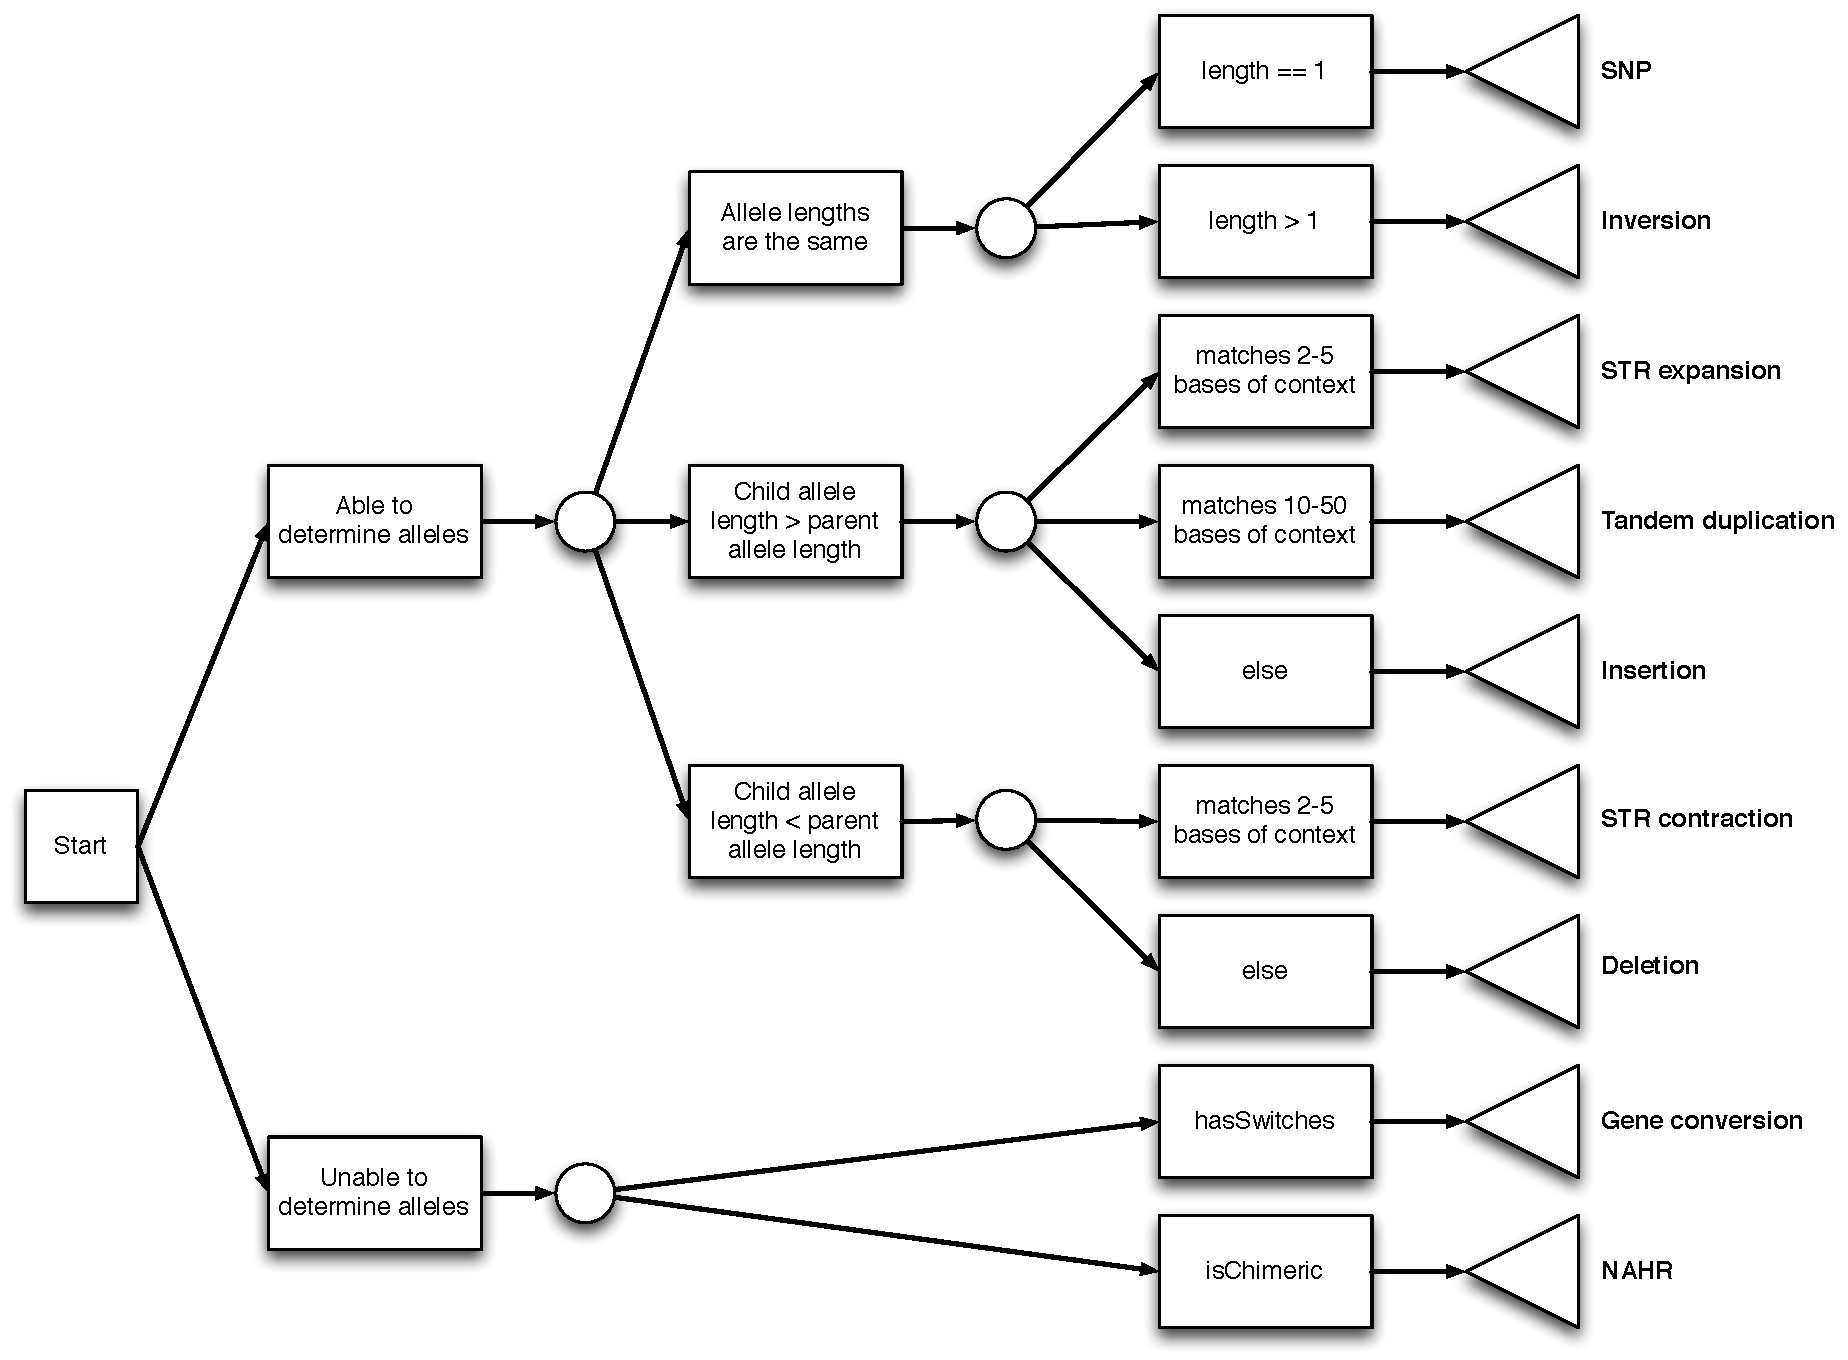
\includegraphics[width=\textwidth]{classification}
  \caption{}
  \label{fig:classification}
\end{figure}

The classification algorithm can be described by the decision tree in Figure \ref{fig:classification}.

\subsubsection{Choosing haplotypic background}

When calling variants, we do not know the haplotypic background upon which a variant has occured.  We must compare the child's graph to the mother's and then to the father's, making separate calls.  This results in two variant calls for the same event.  A single event must be chosen.  In cases where the child and parental alleles are identical, this is trivial.  Additionally, variants where the event can be identified against one parent but not the other are straightforward.  The problematic events are those that have conflicting descriptions between parents.  In this situation, we heuristically assign a score for various properties of the variant, choosing the representation with the highest score.  This has the effect of preferring simpler descriptions (e.g. "SNP") to more complex ones (e.g. "GC").

\begin{algorithm}
\caption{Score variant}
\label{alg:scoreVariant}
\begin{algorithmic}
\Function{chooseVariant}{gvc}
    \State scores = []

    \ForAll{colors c}
        \If{(gvc.traversalIsComplete(c))}
            \State scores[c]++
        \EndIf
        \If{(gvc.variantType(c) != "unknown"}
            \State scores[c]++
        \EndIf
        \If{(gvc.variantType(c) not in ("GC", "NAHR"))}
            \State scores[c]++
        \EndIf
    \EndFor

    \State bestColor = whichMax(scores)

    \State return (scores[0] == scores[1] ? 0 : bestColor)
\EndFunction
\end{algorithmic}
\end{algorithm}

\subsubsection{Mark traversed novel kmers as used}

We then mark all the novel kmers we saw used in the stretch as used so we do not process them again.  This allows us to keep track of our progress, only acting on kmers that have not been associated to any variant yet.

\subsection{Evaluate performance}

We evaluated the performance of our graphical DNM caller by running the thing on some simulated data.  Note that the way a variant is simulated and the way a variant is called are not necessarily identical.  In particular, indels are tricky because there is not a standard representation in graphs.  Usually, when indels are called in reference-based methods, the reference is taken to be the forward strand and indels are left-shifted as far as possible.  In graphs, there is no information available for determining orientation.  When they were simulated, we knew what the forward strand was, but we do not know that in the graph.  Thus, when we go to check on the presence of a variant, we must check it in both orientations, and accounting for multiple representations.

\subsubsection{Pre-compute novel kmer to variant map}

We iterated through all variants, extracting sequence from the simulated child's reference genome between $\textrm{start} - (2k - 1)$ and $\textrm{stop} + (2k - 1)$ bp.  We then extracted each kmer from this sequence and, if the kmer is novel, emitting a table row mapping the novel kmer to variant ID, variant type, and position in the child's reference genome.  Note that because we chose to space our variants out over considerable distance, it is generally not possible for a kmer to map to multiple variants.  However, as we have placed very few constraints on variant positioning otherwise, it is possible a simulated variant has landed in a low-complexity region that occurs multiple times throughout the genome, and that multiple variants thus share novel kmers.  In that instance, the first variant we see during processing is assigned the novel kmer.

\subsubsection{Load variant containing a novel kmer and comparing}

If we are in evaluation mode (that is, if we've a novel kmer to variant map along with a dataset), then after each variant we call, we check if any of the kmers involved in the variant call are in the map, and load the relevant variant information.  We then evaluate our call using Algorithm \ref{alg:evalVariant}.

\begin{algorithm}
\caption{Evaluate variant}
\label{alg:evalVariant}
\begin{algorithmic}
\Function{evalVariant}{call, truth, stretch}
    \State relevantVariants = []

    \ForAll{kmers in stretch}
        \If{(truth.contains(kmer))}
            \State push(relevantVariants, truth.get(kmer))
        \EndIf
    \EndFor

    \State bestVariant = null;
    \ForAll{vi in relevantVariants}
        \State ref = call.getParentalAllele()
        \State alt = call.getChildAllele()

        \State refStretch = call.getParentalStretch()
        \State altStretch = call.getChildStretch()

        \State found = false;

        \If{(!found)}
            \Comment left-shift variants and check
            \State pos = call.getStart()

            \While{(pos >= 0 \&\& pos + ref.length() < refStretch.length() \&\& pos + alt.length() < altStretch.length())}
                \State refFw = refStretch.substring(pos, pos + ref.length())
                \State altFw = altStretch.substring(pos, pos + altLength)

                \State refRc = reverseComplement(refFw);
                \State altRc = reverseComplement(altFw)

                \If{(known ref and alt alleles match called fw or rc alleles)}
                    \State ref = (refFw or refRc)
                    \State alt = (altFw or altRc)
                    \State found = true;
                    \State break;
                \EndIf

                \State pos--
            \EndWhile
        \EndIf

        \If{(!found)}
            \Comment right-shift variants and check
            \State pos = call.getStart()

            \While{(pos >= 0 \&\& pos + ref.length() < refStretch.length() \&\& pos + alt.length() < altStretch.length())}
                \State refFw = refStretch.substring(pos, pos + refLength)
                \State refRc = reverseComplement(refFw)

                \State altFw = altStretch.substring(pos, pos + altLength)
                \State altRc = reverseComplement(altFw)

                \If{(known ref and alt alleles match called fw or rc alleles)}
                    \State ref = (refFw or refRc)
                    \State alt = (altFw or altRc)
                    \State found = true;
                    \State break;
                \EndIf

                \State pos++
            \EndWhile
        \EndIf

        \Comment Maybe what we've found is a truncated version of what we were expecting
        \State knownRef = vi.ref
        \State knownAlt = vi.alt == null ? "" : vi.alt

        \If{(!found \&\& knownRef.length() > ref.length() \&\& knownAlt.length() > alt.length() \&\& knownRef.length() == knownAlt.length())}
            \State refFw = ref;
            \State altFw = alt;
            \State refRc = reverseComplement(refFw);
            \State altRc = reverseComplement(altFw);

            \State refFinal = null, altFinal = null;

            \If{(knownRef contains refFw or refRc and knownAlt contains altFw or altRc)}
                \State refFinal = (refFw or refRc)
                \State altFinal = (altFw or altRc)
            \EndIf

            \If{(refFinal != null \&\& altFinal != null)}
                \State r0index = knownRef.indexOf(refFinal)
                \State a0index = knownAlt.indexOf(altFinal)
                \State r1index = r0index + refFinal.length()
                \State a1index = a0index + altFinal.length()

                \If{(r0index == a0index \&\& r1index == a1index \&\&
                        knownRef.substring(0, r0index).equals(knownAlt.substring(0, a0index)) \&\&
                        knownRef.substring(r1index, knownRef.length()).equals(knownAlt.substring(a1index, knownAlt.length())))}
                    knownRef = ref;
                    knownAlt = alt;
                \EndIf
            \EndIf
        \EndIf

        \State vi.found = true;
        \State vi.matches = (knownRef.equals(ref) \&\& knownAlt.equals(alt)) || vi.type.equals(call.getType())

        \If{(bestVi == null || vi.matches)}
            \State bestVi = vi;
        \EndIf

        \If{(bestVi != null)}
            \State knownRef = bestVi.ref;
            \State knownAlt = bestVi.alt != null ? bestVi.alt : "";
        \EndIf
    \EndFor
\EndFunction
\end{algorithmic}
\end{algorithm}

\section{Results on simulated data}

We ran our algorithm on the perfect and realistic simulated datasets presented in Chapter \ref{ch:simulation}.  Looking first at purely event recovery without classification (i.e. did we find \textit{de novo} variants, irrespective of whether we classified them correctly), we summarize our stats in Tables \ref{tbl:roc_perfect} and \ref{tbl:roc_realistic}.  In both cases, our sensitivity and specificity to DNMs is very high - greater than $98\%$ in nearly all cases.  Note that the true negatives (tn) are effectively every kmer that we did \textit{not} call in our dataset, which effecitvely makes our specificity nearly perfect, as the use of the novel kmers prevents us from making calls in the vast majority of the graph.

Additionally in these tables, we also computed the "redundant call", or "rc" metric.  The rc metric reveals an important caveat regarding graph calls: should the traversals fail and the alleles of the variant not ascertained, the novel kmers involved in the variant will not be marked as used.  However, we still emit a variant "event", despite our inability to classify it.  In the subsequent iteration of the algorithm, the remaining novel kmers will be picked up for calling again, leading to the same variant being emitted multiple times.  Thus, we must exercise caution with untyped variants: the rate at which they appear in our callset may be slightly higher (up to $10\%$) than the rate at which they truly exist in the genome.

\begin{sidewaystable}[]
\centering
\caption{ROC metrics on simulated perfect data}
\label{tbl:roc_perfect}
\begin{tabular}{rlrrrrrrrrrrrrr}
\toprule
sn & sim & fp & fn & tp & tn & rc & sens & spec & prec & npv & fpr & fnr & fdr & acc\\
\midrule
5 & perfect & 1 & 5 & 126 & 22240910 & 9 & 0.9618 & 1 & 0.9921 & 1 & 0 & 0.0382 & 0.0079 & 1\\
3 & perfect & 2 & 3 & 154 & 22200660 & 4 & 0.9809 & 1 & 0.9872 & 1 & 0 & 0.0191 & 0.0128 & 1\\
0 & perfect & 0 & 2 & 106 & 22241343 & 7 & 0.9815 & 1 & 1.0000 & 1 & 0 & 0.0185 & 0.0000 & 1\\
12 & perfect & 0 & 2 & 113 & 22233659 & 3 & 0.9826 & 1 & 1.0000 & 1 & 0 & 0.0174 & 0.0000 & 1\\
13 & perfect & 0 & 2 & 114 & 22217297 & 5 & 0.9828 & 1 & 1.0000 & 1 & 0 & 0.0172 & 0.0000 & 1\\
17 & perfect & 0 & 2 & 117 & 22242890 & 6 & 0.9832 & 1 & 1.0000 & 1 & 0 & 0.0168 & 0.0000 & 1\\
1 & perfect & 1 & 2 & 137 & 22249556 & 8 & 0.9856 & 1 & 0.9928 & 1 & 0 & 0.0144 & 0.0072 & 1\\
14 & perfect & 2 & 2 & 162 & 22196410 & 7 & 0.9878 & 1 & 0.9878 & 1 & 0 & 0.0122 & 0.0122 & 1\\
11 & perfect & 1 & 1 & 114 & 22207761 & 2 & 0.9913 & 1 & 0.9913 & 1 & 0 & 0.0087 & 0.0087 & 1\\
6 & perfect & 1 & 1 & 118 & 22203683 & 2 & 0.9916 & 1 & 0.9916 & 1 & 0 & 0.0084 & 0.0084 & 1\\
8 & perfect & 1 & 1 & 129 & 22229379 & 5 & 0.9923 & 1 & 0.9923 & 1 & 0 & 0.0077 & 0.0077 & 1\\
10 & perfect & 0 & 1 & 130 & 22238480 & 2 & 0.9924 & 1 & 1.0000 & 1 & 0 & 0.0076 & 0.0000 & 1\\
15 & perfect & 1 & 1 & 131 & 22208991 & 10 & 0.9924 & 1 & 0.9924 & 1 & 0 & 0.0076 & 0.0076 & 1\\
16 & perfect & 1 & 1 & 166 & 22213928 & 4 & 0.9940 & 1 & 0.9940 & 1 & 0 & 0.0060 & 0.0060 & 1\\
2 & perfect & 1 & 0 & 105 & 22225262 & 3 & 1.0000 & 1 & 0.9906 & 1 & 0 & 0.0000 & 0.0094 & 1\\
4 & perfect & 2 & 0 & 72 & 22210167 & 2 & 1.0000 & 1 & 0.9730 & 1 & 0 & 0.0000 & 0.0270 & 1\\
7 & perfect & 1 & 0 & 57 & 22225612 & 1 & 1.0000 & 1 & 0.9828 & 1 & 0 & 0.0000 & 0.0172 & 1\\
9 & perfect & 0 & 0 & 107 & 22255460 & 2 & 1.0000 & 1 & 1.0000 & 1 & 0 & 0.0000 & 0.0000 & 1\\
18 & perfect & 2 & 0 & 133 & 22242522 & 0 & 1.0000 & 1 & 0.9852 & 1 & 0 & 0.0000 & 0.0148 & 1\\
19 & perfect & 1 & 0 & 98 & 22236313 & 6 & 1.0000 & 1 & 0.9899 & 1 & 0 & 0.0000 & 0.0101 & 1\\
\bottomrule
\end{tabular}
\end{sidewaystable}

\begin{sidewaystable}[]
\centering
\caption{ROC metrics on simulated realistic data}
\label{tbl:roc_realistic}
\begin{tabular}{rlrrrrrrrrrrrrr}
\toprule
sn & sim & fp & fn & tp & tn & rc & sens & spec & prec & npv & fpr & fnr & fdr & acc\\
\midrule
5 & realistic & 4 & 2 & 123 & 77566161 & 7 & 0.9840 & 1 & 0.9685 & 1 & 0 & 0.0160 & 0.0315 & 1\\
0 & realistic & 1 & 1 & 101 & 77516712 & 7 & 0.9902 & 1 & 0.9902 & 1 & 0 & 0.0098 & 0.0098 & 1\\
6 & realistic & 2 & 1 & 107 & 77289511 & 2 & 0.9907 & 1 & 0.9817 & 1 & 0 & 0.0093 & 0.0183 & 1\\
13 & realistic & 0 & 1 & 107 & 77362132 & 3 & 0.9907 & 1 & 1.0000 & 1 & 0 & 0.0093 & 0.0000 & 1\\
17 & realistic & 3 & 1 & 109 & 77390562 & 5 & 0.9909 & 1 & 0.9732 & 1 & 0 & 0.0091 & 0.0268 & 1\\
12 & realistic & 2 & 1 & 111 & 77440516 & 3 & 0.9911 & 1 & 0.9823 & 1 & 0 & 0.0089 & 0.0177 & 1\\
16 & realistic & 1 & 1 & 155 & 77369055 & 5 & 0.9936 & 1 & 0.9936 & 1 & 0 & 0.0064 & 0.0064 & 1\\
2 & realistic & 4 & 0 & 93 & 77425427 & 1 & 1.0000 & 1 & 0.9588 & 1 & 0 & 0.0000 & 0.0412 & 1\\
4 & realistic & 3 & 0 & 65 & 77312705 & 2 & 1.0000 & 1 & 0.9559 & 1 & 0 & 0.0000 & 0.0441 & 1\\
3 & realistic & 6 & 0 & 150 & 77296380 & 1 & 1.0000 & 1 & 0.9615 & 1 & 0 & 0.0000 & 0.0385 & 1\\
1 & realistic & 1 & 0 & 133 & 77509177 & 5 & 1.0000 & 1 & 0.9925 & 1 & 0 & 0.0000 & 0.0075 & 1\\
7 & realistic & 4 & 0 & 56 & 77445270 & 1 & 1.0000 & 1 & 0.9333 & 1 & 0 & 0.0000 & 0.0667 & 1\\
8 & realistic & 6 & 0 & 126 & 77469034 & 3 & 1.0000 & 1 & 0.9545 & 1 & 0 & 0.0000 & 0.0455 & 1\\
9 & realistic & 2 & 0 & 95 & 77503142 & 2 & 1.0000 & 1 & 0.9794 & 1 & 0 & 0.0000 & 0.0206 & 1\\
10 & realistic & 1 & 0 & 124 & 77398963 & 2 & 1.0000 & 1 & 0.9920 & 1 & 0 & 0.0000 & 0.0080 & 1\\
11 & realistic & 2 & 0 & 108 & 77422535 & 2 & 1.0000 & 1 & 0.9818 & 1 & 0 & 0.0000 & 0.0182 & 1\\
14 & realistic & 6 & 0 & 150 & 77355056 & 7 & 1.0000 & 1 & 0.9615 & 1 & 0 & 0.0000 & 0.0385 & 1\\
15 & realistic & 1 & 0 & 125 & 77435743 & 9 & 1.0000 & 1 & 0.9921 & 1 & 0 & 0.0000 & 0.0079 & 1\\
18 & realistic & 4 & 0 & 123 & 77355144 & 3 & 1.0000 & 1 & 0.9685 & 1 & 0 & 0.0000 & 0.0315 & 1\\
19 & realistic & 2 & 0 & 95 & 77480228 & 6 & 1.0000 & 1 & 0.9794 & 1 & 0 & 0.0000 & 0.0206 & 1\\
\bottomrule
\end{tabular}
\end{sidewaystable}

\begin{figure}[h!]
  \centering
    \includegraphics[width=\textwidth]{{conf.perfect.hm-1}.pdf}
  \caption{Confusion matrix for observed events (below) versus expected events (right), in simulated perfect data.}
  \label{fig:conf_perfect_hm}
\end{figure}

\begin{figure}[h!]
  \centering
    \includegraphics[width=\textwidth]{{conf.realistic.hm-1}.pdf}
  \caption{Confusion matrix for observed events (below) versus expected events (right), in simulated realistic data.}
  \label{fig:conf_realistic_hm}
\end{figure}

Results on event classification are shown as heatmaps in Figures \ref{fig:conf_perfect_hm} and \ref{fig:conf_realistic_hm}, with observed events on the bottom and expected events on the side.  On the observed axis, an "unknown" event denotes a variant that could not be typed.  On the expected axis, an "unknown" event is one that does not appear in the simulation list (i.e. a false positive).  The total number of events simulated that could possibly be recovered via novel kmers is the sum of each row (except for the "unknown" row, which instead enumerates the false positives and the types they've been assigned).  For the most part, variants appear on the diagonal, indicating proper classification.  Performance degrades when we move into the non-bubble motif variants (i.e. GC and NAHR) events.

Gene conversion events are quite often erroneously described as SNPs.  This is likely due to the fact that the classification algorithm is looking for clear switches of parental copying in the child (copying from mother, then father, then mother again, or vice versa).  However, if variants that appear on different haplotypic backgrounds are too close to one another, $47$-bp kmers might span both, and the recombination motif that we seek may be obscured and cause the algorithm to call a SNP instead.

Many NAHR events are classified as "unknown".  This is perhaps not unreasonable.  Our classification algorithm for NAHR events (Algorithm \ref{alg:hasChimeras}) requires that the stretch have kmers from different chromosomes.  However, if the stretch truncates early due to errors or homology, there may be insufficient genomic context in order to determine the chromosomes of origin, leaving us unable to classify the variant accordingly.

\section{Summary}

We have presented our algorithms for identifying and typing \textit{de novo} variation in cross/pedigree data.  At the heart of our approach is a graphical model based on a de Bruijn graph representation of sequencing data from parents and children.  We exploit the novel kmer generation property of DNMs to discover regions of the graph worth exploring for DNM activity, being careful to discard kmers seemingly arising from error.  This approach appears to work well in simulation, typically recovering bubble-motif events well and exhibiting predicted difficulty with more complex, linear-motif events (those involving some form of recombination).

\chapter{\textit{Real data}}
\label{ch:pf}

\begin{figure}[h!]
  \centering
    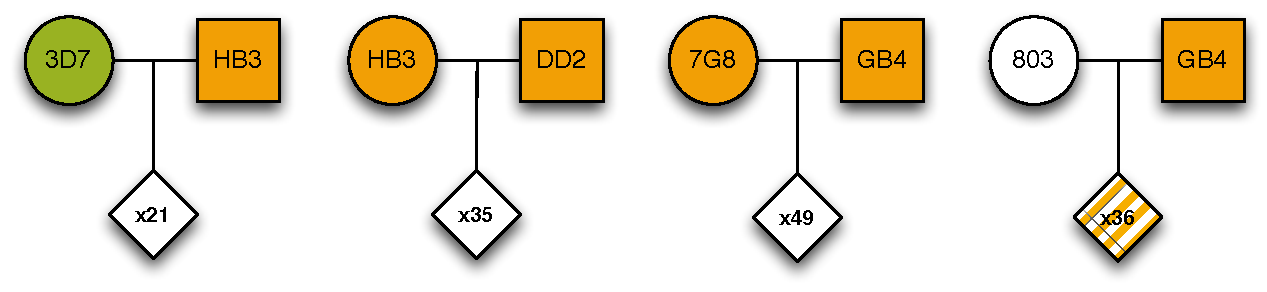
\includegraphics[width=0.9\textwidth]{pfpedigree}
  \caption{Relationships for samples in four \textit{P. falciparum} crosses, with the number of QC-passing Illumina datasets for progeny shown.  Green and orange shading indicates the availability of finished and draft quality reference genomes, respectively.  Orange stripes denote the availability of a draft reference genome for a single progeny, used as validation for \textit{de novo} events.  Gender assignments for the parents are arbitrary, intended only to simplify discussion.}
  \label{fig:pfpedigree}
\end{figure}

\newthought{In the previous chapter, we demonstrated our \textit{de novo} mutation detection} software on simulated crossings of \textit{Plasmodium falciparum} malaria parasites.  We now apply our work to real samples: short-read Illumina data on nearly $150$ isolates taken from four separate crossings of six parasites.

No comprehensive catalog of \textit{de novo} variation in these crosses currently exists.  To date, the focus on the $3D7xHB3$, $HB3xDD2$, $7G8xGB4$ and $803xGB4$ datasets has primarily been on discovering the genomic basis for phenotypic differences between the parents, and on characterizing novel antigenic forms in the children.  However, the previous phenotypic studies have verified the presence of some large structural \textit{de novo} variants - namely a handful of NAHR events involving antigenic genes.  These known events serve as useful validation data for the most difficult form of variation for our software to detect.  Furthermore, these previously observed events have occurred in low-complexity regions.  These regions may confound DNA repair machinery and provide a substrate for the generation of \textit{de novo} variation.  They are typically considered outside the reach of reference-based analyses (which constrain themselves to the roughly $20$ megabases of so-called "core" genome wherein divergence between multiple isolates is much lower and short reads tend to align unambiguously\cite{Miles:2015in}), but may be accessible with our graph-based approach.  Finally, the \textit{P. falciparum} genome is small enough to be sequenced inexpensively on current third generation sequencing platforms, enabling high-quality reconstructions of the parental genomes and even one of the progeny.  The parental samples facilitate DNM discovery, while the child sample serves as a validation dataset with which to evaluate our performance.  These factors make the \textit{P. falciparum} datasets a compelling study target.

\section{Data processing}

\subsection{Initial data}

\begin{table}[]
\centering
\caption{Summary of sequencing data for four \textit{Plasmodium falciparum} crosses}
\label{tbl:crosssummary}
\begin{tabular}{@{}lllll@{}}
\toprule
                & 3D7xHB3       & HB3xDD2       & 7G8xGB4       & 803xGB4             \\ \midrule
Samples         & $22$          & $42$          & $52$          & $36$                \\
Samples QC+     & $21$          & $35$          & $49$          & $36$                \\
Read length     & $76$          & $76$          & $76$          & $100$               \\
Fragment size   & $300 \pm 29$  & $253 \pm 48$  & $293 \pm 21$  & $222 \pm 10$        \\
Coverage        & $99  \pm 38$  & $121 \pm 91$  & $110 \pm 40$  & $205 \pm 106$       \\
Platform        & Illumina GAII & Illumina GAII & Illumina GAII & Illumina HiSeq 2000 \\
Sequencing Date & 2010          & 2009-2012     & 2010-2011     & 2014                \\ \bottomrule
\end{tabular}
\end{table}

We obtained short-read, paired-end whole genome sequence data for parent and progeny clones of the $3D7xHB3$\cite{Walliker:1987cv}, $HB3xDD2$\cite{Wellems:1990eg}, $7G8xGB4$\cite{Hayton:2008hn}, and $803xGB4$ crosses, generously provided to us by the MalariaGen project\footnote{More information, including links to the European Nucleotide Archive where the original reads are stored, can be found at \url{http://www.malariagen.net/apps/pf-crosses/1.0/}.  Note that while the 803xGB4 data we were provided does come to us via MalariaGen, it was provided to them (and subsequently to us) as a personal communication from Michael Krause, Rick Fairhurst \textit{et al.} at the NIAID.  It is not yet part of the public dataset.}.  All samples were sequenced on Illumina platforms over the past five years using a PCR-free library preparation protocol known to reduce coverage biases associated with AT-rich templates.  Avoiding PCR during library construction also removes the issue of replication errors that occur in early cycles being propagated to all subsequent copies, thus masquerading as \textit{de novo} mutations.  Across all four crosses, we obtained $152$ samples prior to any quality control checks.  The data is summarized in Table \ref{tbl:crosssummary}.

\subsection{Data processing for progeny}

\subsubsection{Graph construction}

We built de Bruijn graph structures from the available Illumina data for each child with McCortex's \texttt{build} command, using a kmer size of $47$ bp and discarding bases with a Phred-scaled quality score\cite{Brockman:2008p231} less than $Q5$.  The "dirty" graph (raw graph structure before any pruning is applied) was cleaned using McCortex's \texttt{clean} command, allowing the software to compute cleaning thresholds automatically, and falling back to trimming contiguous regions of the graph with coverage less than $2$ in the event that automatic thresholds could not be calculated.  McCortex's contigs, while strictly speaking not used in our analysis, still serve a useful function in quality control checks.  To generate contigs, paired-end reads were thread through the graph with the McCortex \texttt{thread} command and specifying a minimum fragment size of $0$ bp, maximum fragment size of $400$ bp, and choosing the software's (more conservative) one-way gap-filling procedure.

\subsection{Data processing for parents}

\subsubsection{Graph construction}

\begin{table}[b]
\centering
\caption{Additional data availability for all \textit{P. falciparum} cross parents}
\label{tbl:reflist}
\begin{tabular}{@{}lllllll@{}}
\toprule
                   & 3D7 & HB3 & DD2 & 7G8 & GB4 & 803 \\ \midrule
Finished reference & x   &     &     &     &     &     \\
PacBio assembly    & x   & x   & x   & x   & x   &     \\
Draft assembly     &     & x   & x   & x   &     &     \\
Illumina data      & x   & x   & x   & x   & x   & x   \\ \bottomrule
\end{tabular}
\end{table}

Constructing the parental graphs was a bit more involved than graphs for the children as there were often additional data sources to incorporate.  For five out of the six parents, we benefitted from the availability of supplementary draft assembly data from the Pf3k project.  These draft assemblies were constructed using version $3.0$ of the Hierarchical Genome Assembly Process (HGAP$3$)\cite{Chin:2013iw}.  Briefly, the pipeline performs error correction via the \texttt{Quiver} module, which aligns two-thirds of the data to the longest third, emitting the consensus base and recomputed quality score at each position.  The corrected data is then assembled with a modified version of the Celera assembler\cite{Myers:1995vm}, an overlap-layout-consensus (OLC) assembler originally designed for use on long Sanger reads.  While such reads were typically $500$ bp in length, read lengths from PacBio RS II instruments are on average $10,000$ to $14,000$ bp in length, sometimes as long as $50,000$ bp, two orders of magnitude longer than the reads used to assemble the finished 3D7 reference.  This data helps in determining parental paths in the graph near variants with fewer ambiguities than Illumina data.  Table \ref{tbl:reflist} shows all additional data used in constructing parental assemblies.

Parental graph construction was performed on each parental data source separately following the same workflow used for the children's graphs.  The separate graphs were then combined into a single graph using McCortex's \texttt{join} command.

For most samples, the finished or draft PacBio assemblies vastly outperform any assembly that could be produced with the Illumina data, and are an excellent basis for localizing events and determining their proximity to genes.  However, as there is no high-quality sequence of the $803$ genome, we were forced to construct one ourselves using the available Illumina data.  After producing the cleaned graph with the McCortex workflow, we applied the software's paired-end read threading and contig emission steps.  The assembly statistics for all six genomes are presented in Table \ref{tbl:refstats}.  The assembly for $803$ is exceedingly poor compared to the other assemblies, as expected from short Illumina reads.  That the total sequence length is more than $2.5$ times larger than a typical \textit{falciparum} parasite is artifactual and discussed further below.

\subsubsection{Transfer of gene models}

We transferred gene models onto the new genomes by examining existing finished and draft reference genomes and their annotation sets, selecting each annotated exon sequence from its corresponding FASTA sequence file, and aligning it to the new genome using BWA.  For 7G8, GB4, and 803, we transferred only the 3D7 annotations obtained from PlasmoDB release $26$\cite{Aurrecoechea:2009hh}.  For DD2 and HB3, additional separate annotations exist from the Broad Institute\footnote{\url{http://www.broadinstitute.org/annotation/genome/plasmodium_falciparum_spp/}}.  These undoubtedly contain better representations of genes divergent from their 3D7 counterparts (particularly antigens).  However, owing to the poor DD2 and HB3 assemblies to which they are associated, the annotations are likely to be incomplete.  We therefore chose to transfer both the 3D7 and DD2 (HB3) annotations onto the new DD2 (HB3) assemblies.  This has resulted in a slight over-annotation of genes in these two genomes, as shown in Table \ref{tbl:refstats}.  This happens when the gene models slightly differ between 3D7 and the target (e.g. exon end definitions differ by as much as a single nucleotide), but refer to the same gene.  Rather than simply choosing one definition, we permit both to remain as the PlasmoDB annotations are continuously maintained and improved, while the Broad's annotations have not been updated since April $2014$.

\begin{table}[]
\centering
\caption{Statistics on all parental assemblies}
\label{tbl:refstats}
\begin{tabular}{@{}lllllll@{}}
\toprule
    & contigs & min length & max length & N50       & total sequence & genes            \\ \midrule
3D7 & 16      & 5,967      & 3,291,936  & 1,687,656 & 23,332,831     & 5,777            \\
DD2 & 16      & 6,094      & 3,257,617  & 1,661,885 & 22,682,339     & 8,284 (3D7, DD2) \\
7G8 & 17      & 6,094      & 3,311,228  & 1,560,458 & 22,832,195     & 5,530 (3D7)      \\
GB4 & 26      & 7,376      & 3,360,747  & 1,565,171 & 23,525,386     & 5,576 (3D7)      \\
HB3 & 28      & 6,094      & 3,378,065  & 1,593,993 & 22,812,563     & 7,467 (3D7, HB3) \\
803 & 148,826 & 47         & 17,610     & 1,042     & 59,118,463     & 4,663 (3D7)      \\ \bottomrule
\end{tabular}
\end{table}

\subsubsection{Generation of visualization resources}

We use the Circos\cite{Krzywinski:2009ix} genomic comparison tool to generate whole-genome views of DNM activity in a sample's genome or in all samples from a single cross.  To prepare these visualizations, we require alignments between the contigs of a parental genome and the chromosomes of the reference.  For 3D7, DD2, 7G8, GB4, and HB3, this is trivial as nearly the entirety of each chromosome has been successfully reconstructed.  For those genomes, we simply lined up each assembled contig with its 3D7 counterpart (at the resolution of the image, details of a true alignment cannot be discerned).  In the case of 803, we aligned each contig to the 3D7 genome using BWA to derive the mapping.  

Finally, we computed a number of sequence composition and complexity metrics in tiled $2,500$ bp windows using the SeqComplex tool\footnote{https://github.com/caballero/SeqComplex}.  The full list of metrics computed is as follows:

\begin{enumerate}
\item gc: GC content
\item gcs: GC skew (defined as $(G - C)/(G + C)$)
\item at: AT content
\item ats: AT skew (defined as $(A - T)/(A + T)$)
\item cpg: CpG content
\item ce: Sequence complexity by Shannon entropy\cite{Shannon:1948iy}
\item cl: Sequence complexity by linguistic values\cite{Trifonov:1990vu}
\item cwf: Sequence complexity by Wootton and Federhen\cite{Wootton:1996tu}
\item cz: Sequence compression factor (the ratio of uncompressed to compressed sequence file size, using the \texttt{gzip} compression utility)
\end{enumerate}

These metrics were computed for each parental genome except 803, whose contig lengths were too variable to consistently satisfy the $2,500$ bp window requirement, making comparison with GB4 cumbersome.

\subsection{Quality control}
We examined assembly metrics on all of our samples in order to flag samples for downstream analysis rejection.  We examined each sample for outlier behavior per cross in the number of unique kmers (total number of unique kmers in the graph after the automatic cleaning step - too few kmers indicate poor sequencing quality resulting in most data being thrown away) and contig N50 (the weighted median length of the contigs - very short contigs may indicate high sequencing error rate).  The number of samples retained for analysis is in Table \ref{tbl:crosssummary}.

One expects that a newly assembled \textit{falciparum} parasite should have a similar assembly length to the $3D7$ reference sequence, or at least the other assembled parasites in this dataset.  While this is true for nearly all samples in the 3D7xHB3, HB3xDD2, and 7G8xGB4 crosses, many of the $803xGB4$ samples, shown in Figure \ref{fig:weirdnessAsmLength}, appear to defy this expectation.  Some (including the $803$ parental sample) exhibit assembly lengths well above the $23$ megabases we expect.  Several samples have assemblies in excess of $40$ megabases.  This outcome is unchanged even when other assembly software (e.g. SGA) is applied.  The source of this excess sequence is unclear, but contamination by an organism not present in the BLAST database is a plausible hypothesis.  We note that during investigation of this phenomenon, an update to our BLAST database revealed a number of kmers from the \textit{Pseudomonas} genus that had previously been considered "novel", as the kmers in question were not yet present in the database.  The \textit{Pseudomonas} genus is a family of common environmental bacterium, one of the leading causes of opportunistic human infection\cite{Stover:2000dy}, and around $6.7$ Mbp in length.  It is the subject of drug resistance surveilence\cite{Winsor:2016ca} at many labs including the Wellcome Trust Sanger Institute, where our \textit{falciparum} samples were processed.

For labs that routinely perform a lot of sequencing, it is common for samples from different projects to be prepared simultaneously, and/or for samples to be multiplexed to maximize the use of sequencer capacity, both of which can contribute to sample cross-contamination\cite{Jun:2012je}.  Assembly software does not typically employ contamination checks prior to assembly, instead simply processing any data provided to it.  It is likely that any such contamination would have been assembled and incorporated mostly as disconnected regions of the de Bruijn graph - a series of vertices that do not connect to any other part of the \textit{falciparum} genome.  This might serve to inflate the novel kmer count if the child sample is contaminated but the parents are not, but such regions are easily identified and discarded.  Therefore, we did not treat inflated assembly size to be a QC failure.

\begin{figure}[h!]
  \centering
    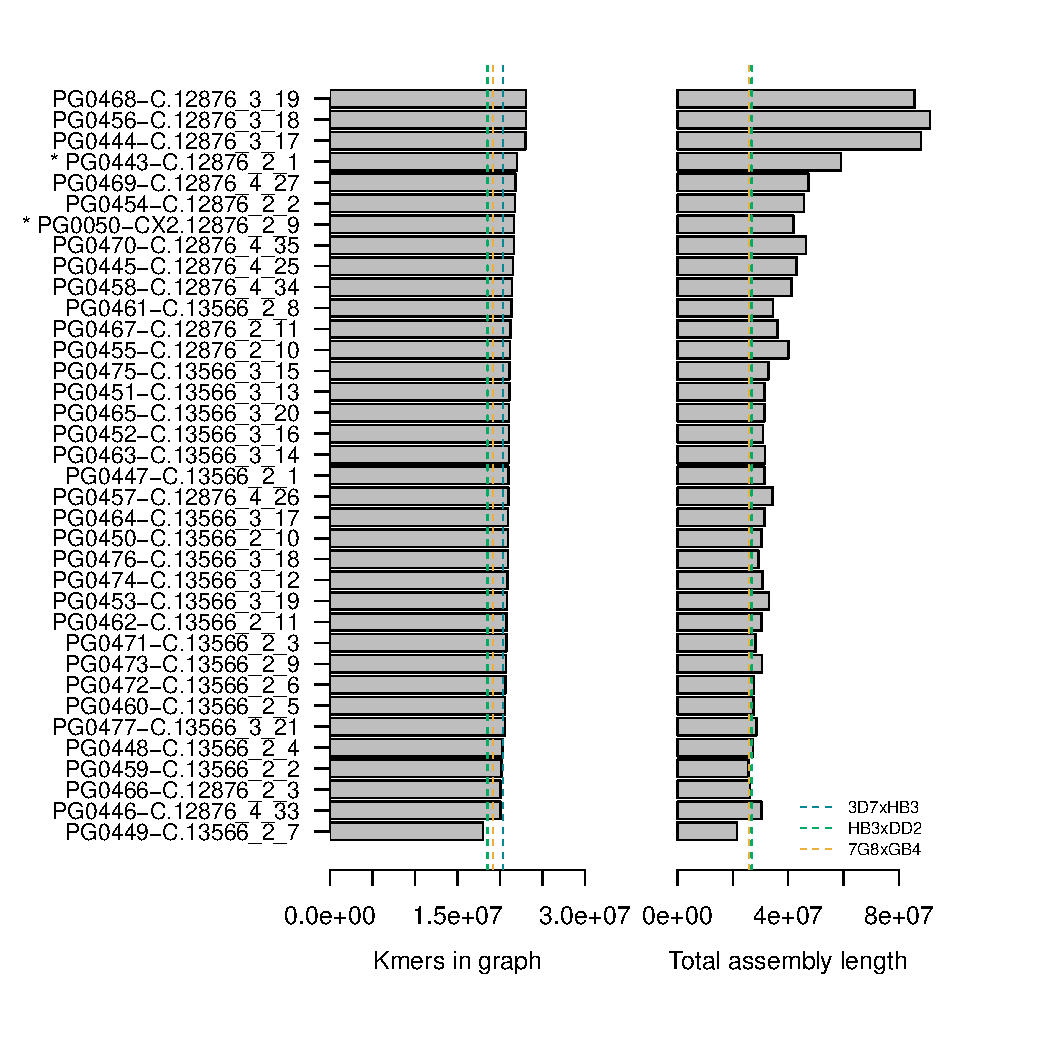
\includegraphics[width=0.5\textwidth]{weirdnessAsmLength-1}
  \caption{Number of kmers and assembly length in the 803xGB4 samples.  Vertical dashed lines indicate the mean value of the metric in other crosses.}
  \label{fig:weirdnessAsmLength}
\end{figure}

\subsection{Data processing for validation isolates}

We selected a number of samples for long-read sequencing on the PacBio RS II instrument.  As of this writing, two samples have been completed: PG0051-C (the 3D7 clone, useful for verifying assembly quality by comparison with the finished 3D7 reference), and PG0446-C (one of the 803xGB4 progeny).  The former was provided by Susana Campino of the Kwiatkowski lab at the Wellcome Trust Sanger Institute.  The latter was provided by Michael Krause and Rick Fairhurst at the Malaria Pathogenesis and Human Immunity Unit at the National Institute of Allergy and Infectious Disease.  Approximately $15~{\mu}g$ of high molecular weight gDNA was provided for each isolate to the CSHL Pacific Biosciences Sequencing Service\footnote{\url{http://cshl.edu/Research/PacBio.html}}.  Sequencing libraries with an average fragment size of $20$ kb were constructed for each sample and size-selected to remove fragments smaller than $7$ kb and larger than $20$ kb using BluePippin.  Optimal loading concentration was determined by choosing a wide range for each of the first $4$ SMRT cells and selecting the concentration that yielded the highest read yield for the remaining SMRT cells.  The PG0051-C isolate was sequenced in late 2014 with the P5-C3 chemistry and assembled with PacBio's HGAP $2.0$ software (assuming a genome size of $23$ megabases).  The PG0446-C isolate, run $16$ months later, was sequenced with the newer P6-C4 chemistry and HGAP $3.0$ software with the same genome size parameter.  Table \ref{tbl:asmstatspacbio} summarizes the sequencing and assembly results on these two isolates.

\begin{table}[]
\centering
\caption{Assembly statistics for PacBio RS II data on PG0051-C and PG0443-C isolates}
\label{tbl:asmstatspacbio}
\begin{tabular}{@{}lll@{}}
\toprule
                        & PG0051-C (3D7)   & PG0443-C (36F11)   \\ \midrule
Chemistry               & P5-C3            & P6-C4              \\
SMRT cells              & $8$              & $9$                \\
Number of reads         & $245,661$        & $282,459$          \\
N50 read length         & $12,968$ bp      & $14,339$ bp        \\
Assembler               & HGAP $2.0$       & HGAP $3.0$         \\
Average contig coverage & $78$x            & $94$x              \\
Polished contigs        & $34$             & $33$               \\ \bottomrule
\end{tabular}
\end{table}

\subsubsection{Establishing assembly quality}
We examined genome recovery and access to massively repetitive sequence (subtelomeric and centromeric regions) that tend to be inaccessible with Illumina sequencing.  PacBio reads were aligned to the finished 3D7 genome using PacBio's \texttt{blasr} long read alignment tool\footnote{\url{https://github.com/PacificBiosciences/blasr}}, while Illumina reads were mapped with the \texttt{bwa mem} tool.  Two such regions in the Illumina and PacBio data for the PG0051-C isolate are shown in Figure \ref{fig:pacbioregions}.  It is evident that the PacBio coverage is roughly uniform across the entire length of the chromosome. In contrast, the Illumina coverage spikes and dips as it moves along, reaching zero coverage in many regions (especially the biologically interesting subtelomeric repetitive regions).

\begin{figure}[h!]
  \centering
    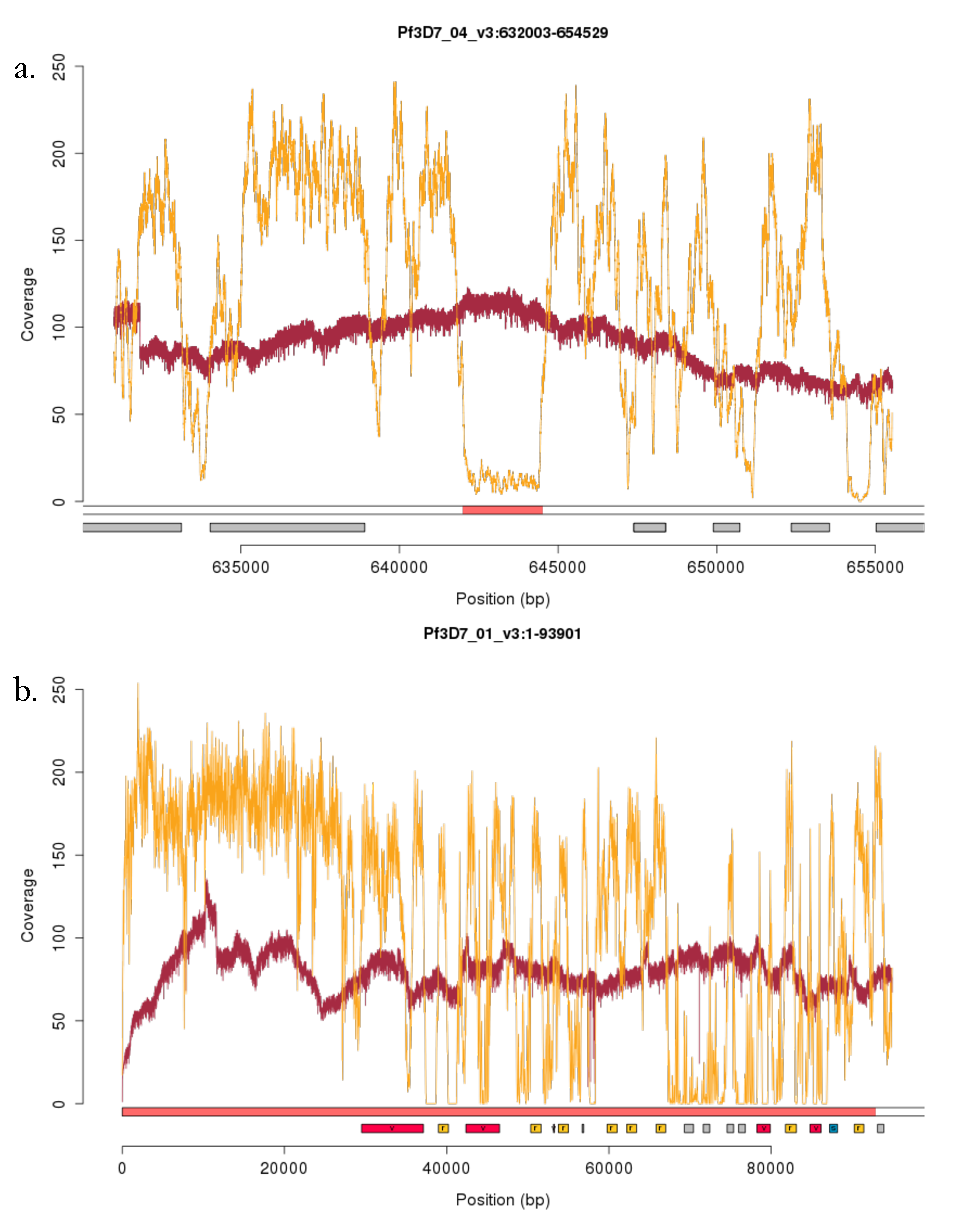
\includegraphics[width=\textwidth]{pacbioregions}
  \caption{Coverage for Illumina data (orange) and PacBio data (red) of the same sample: PG0051-C (the reference isolate, 3D7).  a. Coverage over the chromosome $4$ centromere.  b. Coverage over the $5'$ telomere of chromosome $1$.  Genes from the \textit{var}, \textit{rifin}, and \textit{stevor} antigenic gene families are highlighted and identified with a "v", "r", or "s", respectively.}
  \label{fig:pacbioregions}
\end{figure}

We compared the PacBio-produced assembly of the PG0051-C isolate to the finished reference sequence by performing an all-by-all (contigs versus chromosomes) alignmnt with MUMmer\cite{Versatileandopens:2004dy}.  The alignments are visualized as a multi-dotplot in Figure \ref{fig:dotplot3D7}, an extension of a dot plot that depicts alignments as two dimensional matricies with target and query sequences on the $x$ and $y$ axes, aligning regions of the two sequences shaded accordingly\cite{Gibbs:1970jf}.  Most chromosomes are assembled completely, and the overwhelming majority of the assembly appears on-diagonal (indicating successful one-to-one reconstruction).  Elements appearing off-diagonal could represent misassembly.  However, note that most of these off-diagonal elements occur towards the extremes of each chromosome.  Given that the reference genome was constructed with Sanger reads substantially shorter than the PacBio reads, it is possible some repetitive regions have been collapsed or misplaced, contributing to this nominal error rate.

\begin{figure}[h!]
  \centering
    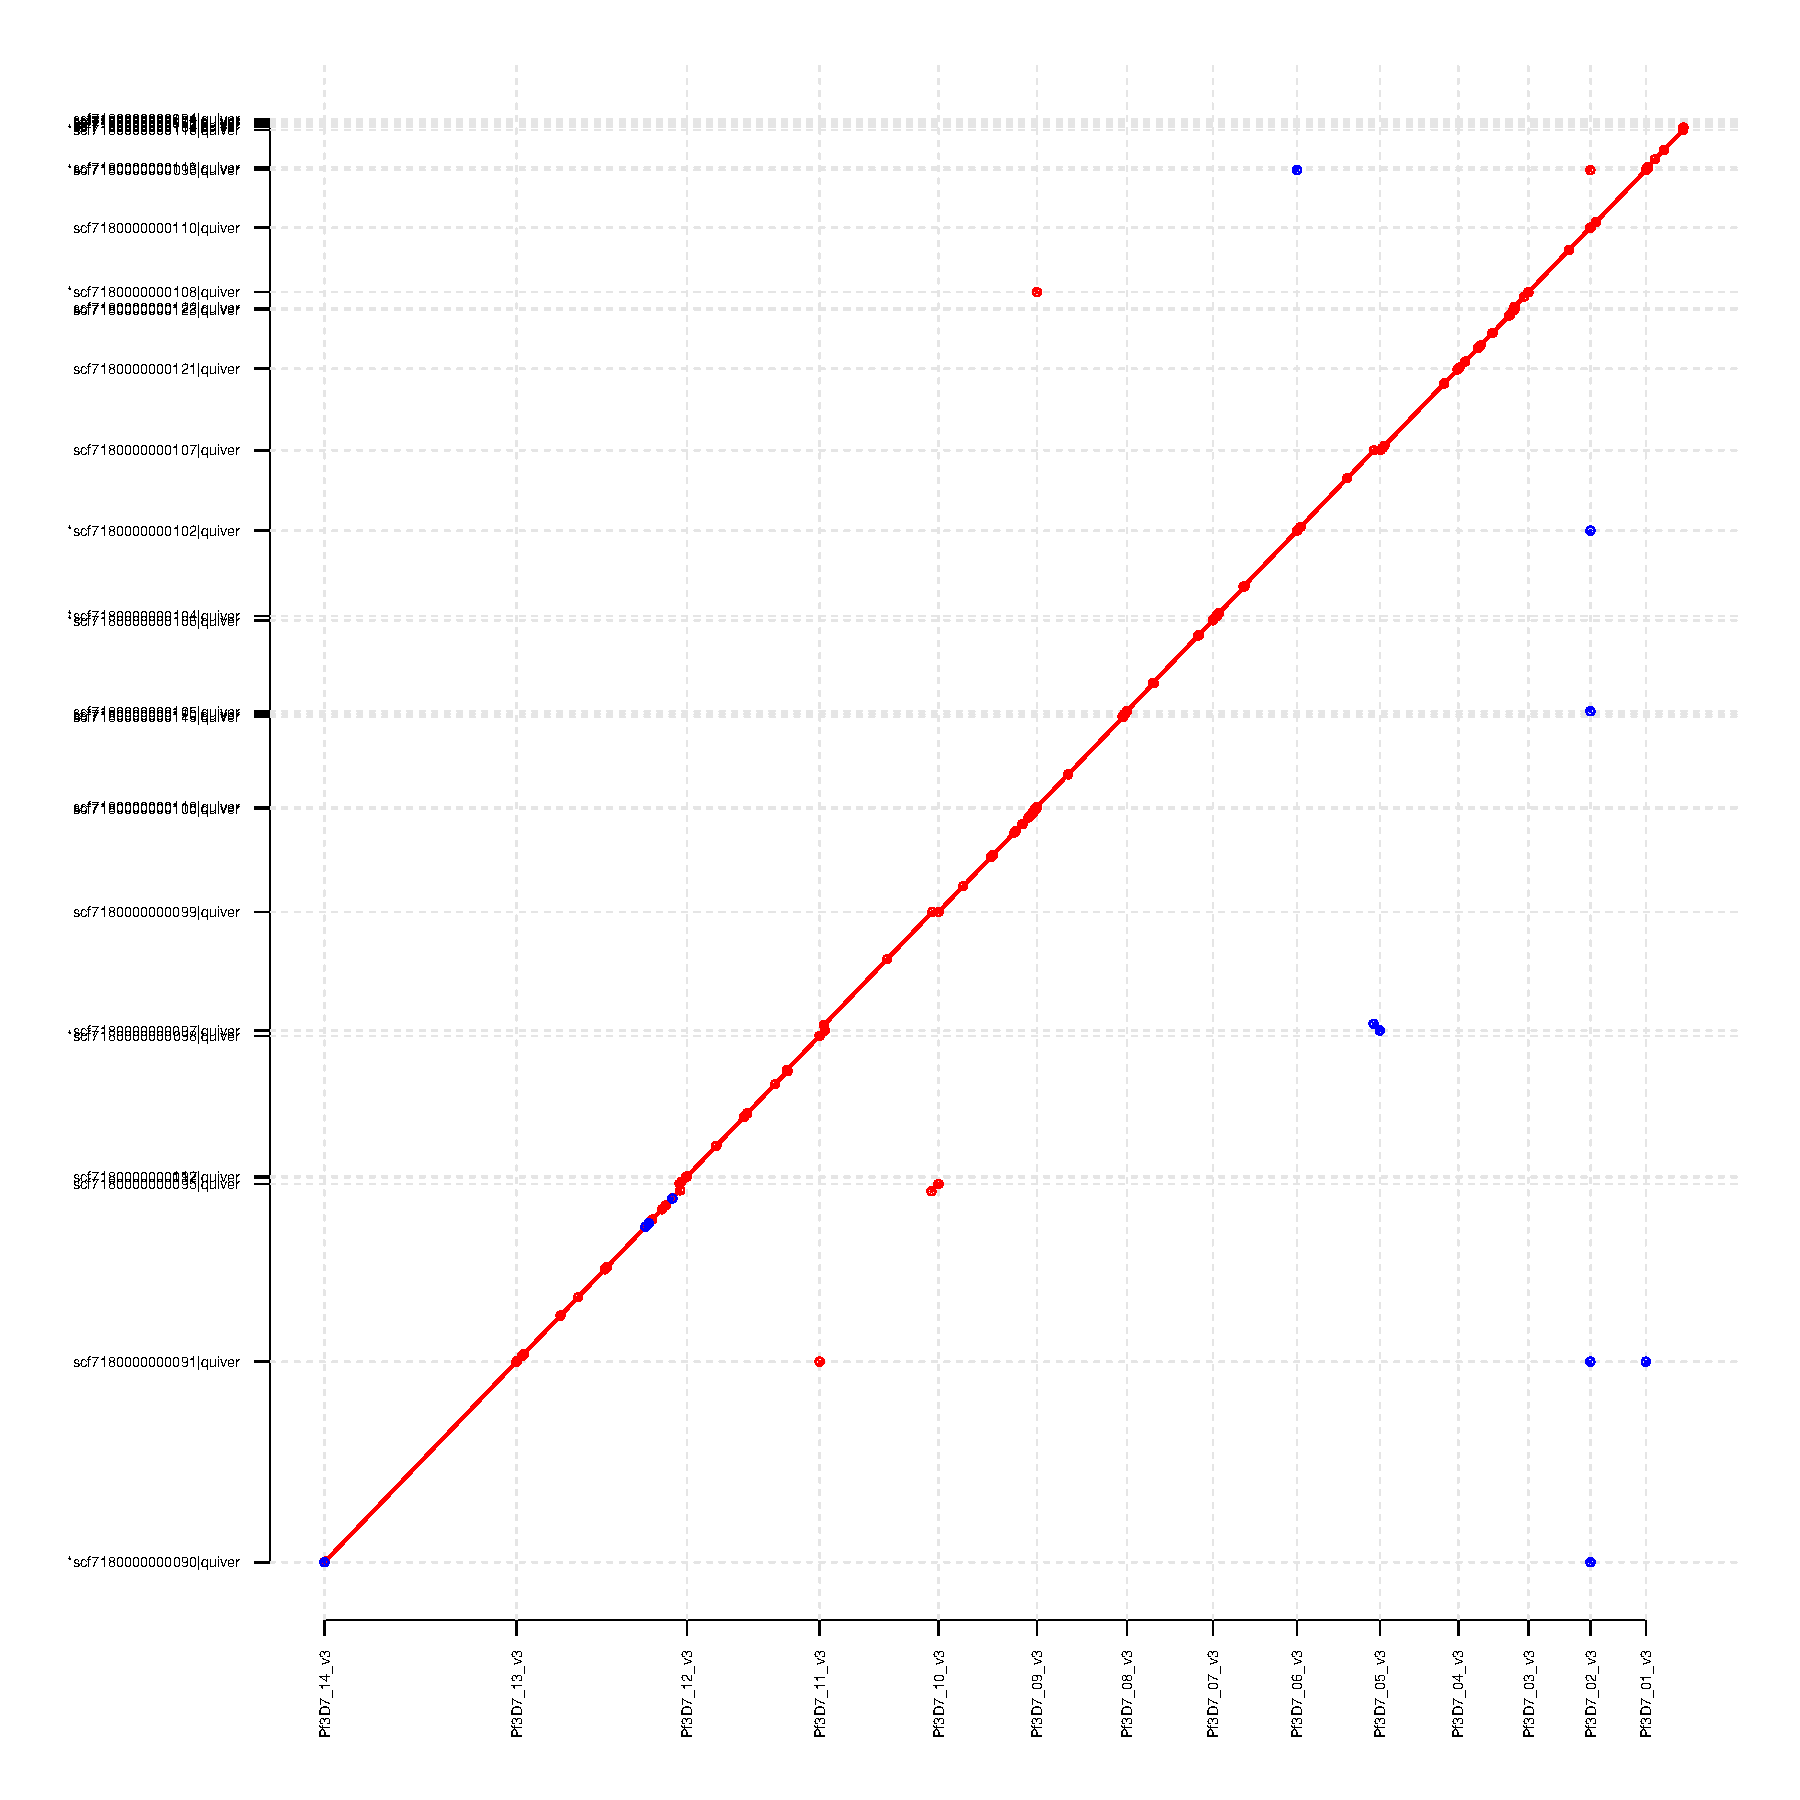
\includegraphics[width=0.7\textwidth]{dotplot}
  \caption{Alignment of contigs from PG0051-C to 3D7 reference assembly}
  \label{fig:dotplot3D7}
\end{figure}

\begin{table}[]
\centering
\caption{Apparent errors per chromosome in the PG0051-C assembly}
\label{tbl:asmerrors}
\begin{tabular}{@{}llll@{}}
\toprule
              & SNP              & INS               & DEL              \\
\midrule
Pf3D7\_01\_v3 & $119~(0.02\%)$   & $763~(0.12\%)$    & $291~(0.05\%)$   \\
Pf3D7\_02\_v3 & $164~(0.02\%)$   & $475~(0.05\%)$    & $162~(0.02\%)$   \\
Pf3D7\_03\_v3 & $272~(0.03\%)$   & $523~(0.05\%)$    & $290~(0.03\%)$   \\
Pf3D7\_04\_v3 & $141~(0.01\%)$   & $856~(0.07\%)$    & $713~(0.06\%)$   \\
Pf3D7\_05\_v3 & $111~(0.01\%)$   & $531~(0.04\%)$    & $175~(0.01\%)$   \\
Pf3D7\_06\_v3 & $504~(0.04\%)$   & $731~(0.05\%)$    & $180~(0.01\%)$   \\
Pf3D7\_07\_v3 & $194~(0.01\%)$   & $609~(0.04\%)$    & $320~(0.02\%)$   \\
Pf3D7\_08\_v3 & $134~(0.01\%)$   & $597~(0.04\%)$    & $251~(0.02\%)$   \\
Pf3D7\_09\_v3 & $61~(0.00\%)$    & $713~(0.05\%)$    & $259~(0.02\%)$   \\
Pf3D7\_10\_v3 & $732~(0.04\%)$   & $810~(0.05\%)$    & $308~(0.02\%)$   \\
Pf3D7\_11\_v3 & $310~(0.02\%)$   & $1,008~(0.05\%)$  & $459~(0.02\%)$   \\
Pf3D7\_12\_v3 & $232~(0.01\%)$   & $1,202~(0.05\%)$  & $390~(0.02\%)$   \\
Pf3D7\_13\_v3 & $231~(0.01\%)$   & $1,493~(0.05\%)$  & $409~(0.01\%)$   \\
Pf3D7\_14\_v3 & $152~(0.00\%)$   & $1,309~(0.04\%)$  & $396~(0.01\%)$   \\
Total         & $3,357~(0.03\%)$ & $11,620~(0.10\%)$ & $4,603~(0.04\%)$ \\
\bottomrule
\end{tabular}
\end{table}

As we have sequenced DNA from the 3D7 parasite, any differences should likely reflect errors in the sequence. We therefore called SNPs between the two assemblies to find these errors. The sums are presented in Table \ref{tbl:asmerrors}, as well as the percent of bases per chromosome these errors represent.  Overall, the SNP, insertion, and deletion rates are exceedingly low: amounting to 19,580 events in a 23 megabase genome (0.17\%). The insertion rate is much higher than that of deletions and SNPs, perhaps due to the dominant insertion error mode of the PacBio sequencing instrument. All chromosomes appear reasonably similar in performance.

We examined the recovery of the $62$ members of the \textit{var} gene family by aligning their full-length genomic sequences (exons and introns) to the PG0051-C assembly using \texttt{bwa mem}. All $62$ \textit{var} genes were successfully aligned to the assembly (all had mapping quality greater than $0$; only $1$ had mapping quality less than 60).  $21$ were found to map with $100\%$ identity. The remaining have, on average, $2.46$ mismatches, $1.39$ insertions, and $0.63$ deletions. The overwhelming majority of indels are a single nucleotide in length.

It seemed likely that many of these errors occur in intronic regions where high repetitive sequence content might contribute to misassembly. We investigated this hypothesis by aligning the exons of the \textit{var} genes separately and enumerating errors observed in exons and introns. We ignored $11$ genes with poor exon alignments (i.e. with mapping quality less than $10$). $91.78\%$ of the errors are found in intronic regions. In all cases, exon $2$ of the \textit{var} gene (the short exon) is base-for-base perfect when compared to the canonical reference.

Based on these measurements of the error rate, we estimate the quality of the PacBio assembly of the PG0051-C (3D7) isolate to be approximately $Q31$\footnote{$Q = -10{\log}_{10}(q) = -10{\log}_{10}((11,620 + 4,603 + 3,357)/23,332,831)$}, or less than one error per thousand bases.  We note that this is a pessimistic estimate, based on the assumption that any differences between this and the reference assembly indicate errors in our assembly.  In long, repetitive regions of the genome, this assumption may not be accurate.

\subsubsection{Preparing the validation isolate reference}

\begin{figure}[h!]
  \centering
    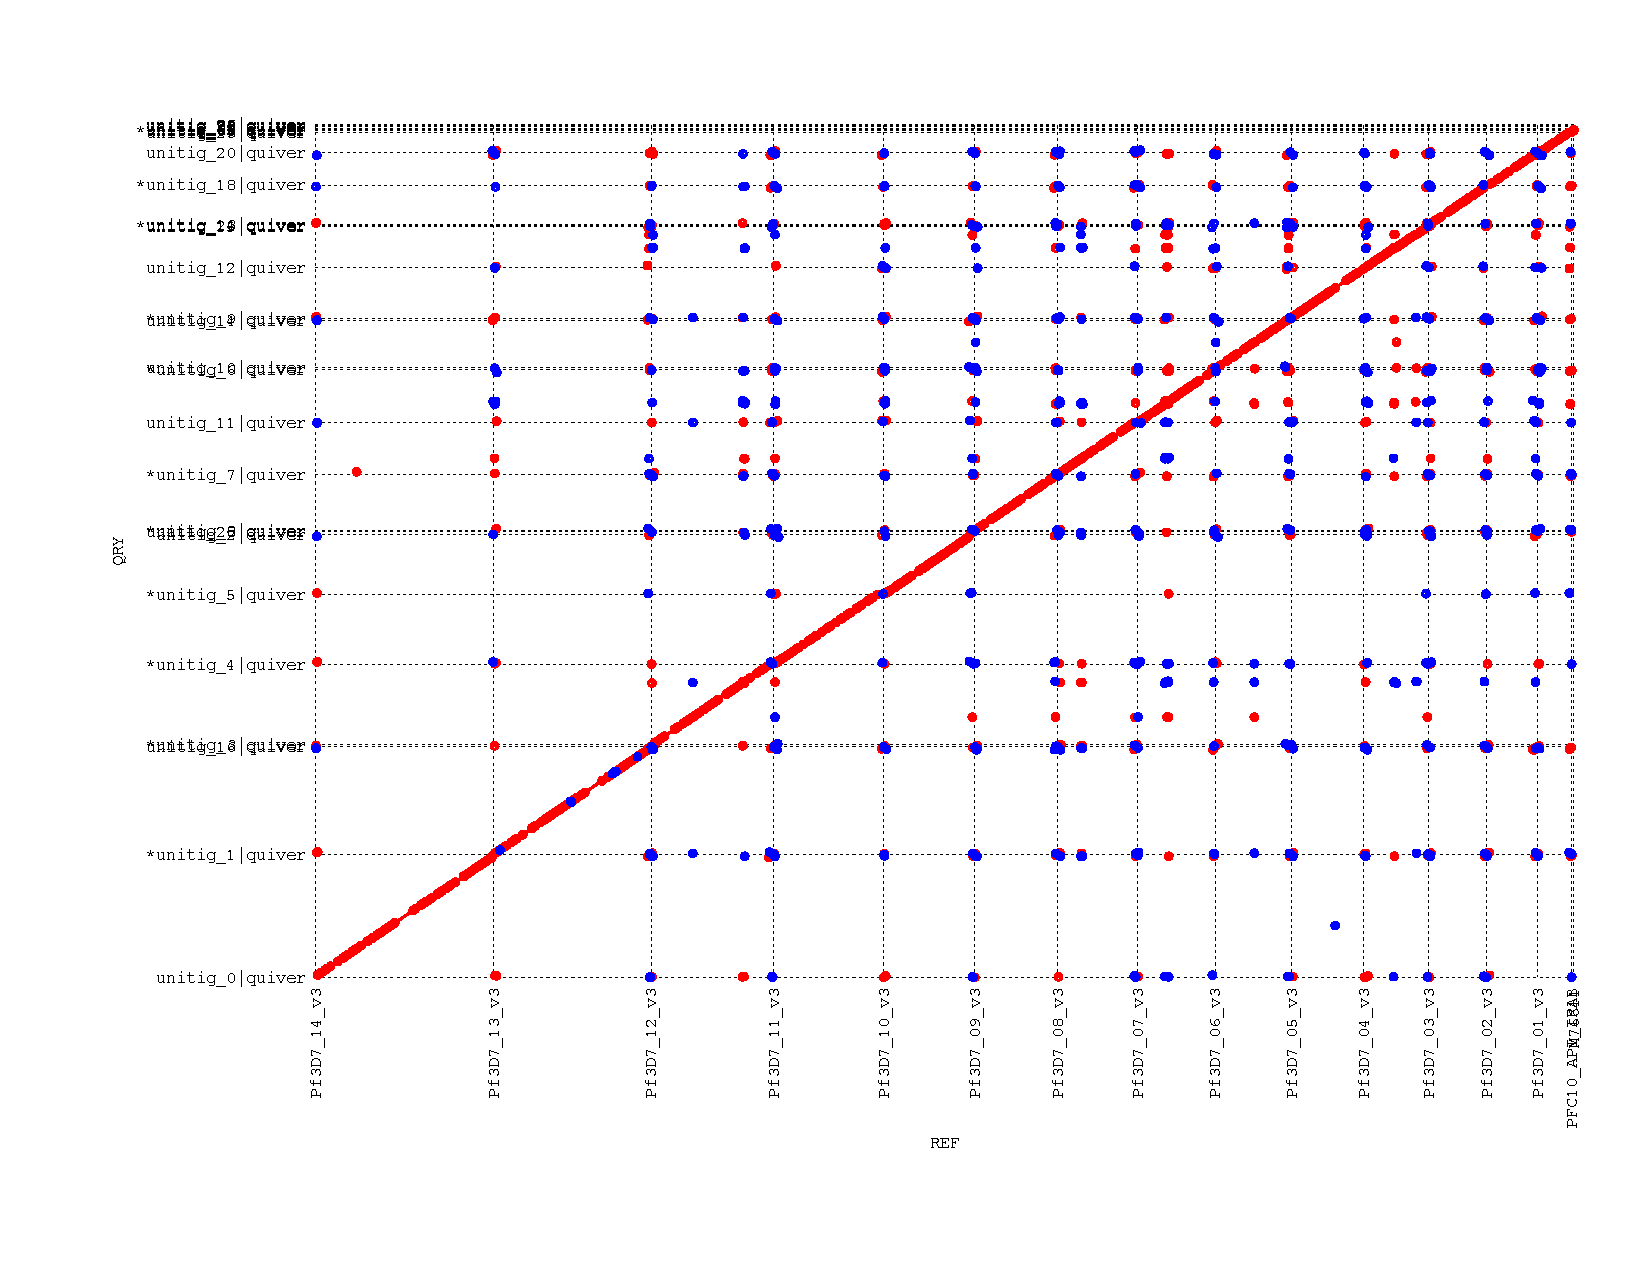
\includegraphics[width=\textwidth]{36F11dotplot}
  \caption{Alignment of contigs from PG0443-C to 3D7 reference assembly}
  \label{fig:valdotplot}
\end{figure}

Having established the performance of the instrument and assembler in providing a viable assembly for a \textit{P. falciparum} isolate, we turned our attention to the validation sample from the 803xGB4 cross, PG0446-C.  We aligned the isolate's assembly to the 3D7 reference sequence using MUMmer, shown in Figure \ref{fig:valdotplot}.  Note that compared to the PG0051-C isolate, the validation isolate has much more off-diagonal activity, particularly towards the telomeres.  This is to be expected.  While the core genome between isolates is expected to be relatively stable, tremendous immune pressure has forced the antigenic repertoire to diversify rapidly.  These genes, primarily located in the subtelomeric regions, are the regions that land off-diagonal, indicative of the extensive recombination and mutation history.

We relabelled and reoriented each contig as necessary based on the alignment so as to more easily establish genomic positioning of events during analysis.  The assignments and orientation were further validated by transferring 3D7 gene model annotations onto the PG0446-C assembly by aligning each exon with \texttt{bwa mem}, operating under the assumption that the core genome is reasonably stable between isolates and that properly labelled and oriented contigs will yield exon alignments that match orientation and approximate positioning between the two assemblies.  Figure \ref{fig:loadGff} shows an example for chromosome $1$.  The vertical offset of all points is due to the fact that the assembly length of chromosome $1$ in the PG0446-C assembly is longer than the reference length.  Only exons towards the telomeric ends of the chromosome are misplaced, evidently originating from chromosomes other than chromosome $1$.  All other chromosome $1$ exons are aligned with the expected position and orientation.

After chromosome identification, we observed a handful of contigs that could not be assigned a place in the nuclear genome.  After running each unplaced contig through BLAST, we discovered two long contigs (thousands of bp) and nearly perfect hits to various species in the \textit{Pseudomonas} genus.  Discovering this contamination in the PacBio assembly and the Illumina samples strongly suggests the samples are contaminated at the source, contributing to the inflated 803xGB4 assembly lengths.  We removed these contigs from our assembly.

\begin{figure}[h!]
  \centering
    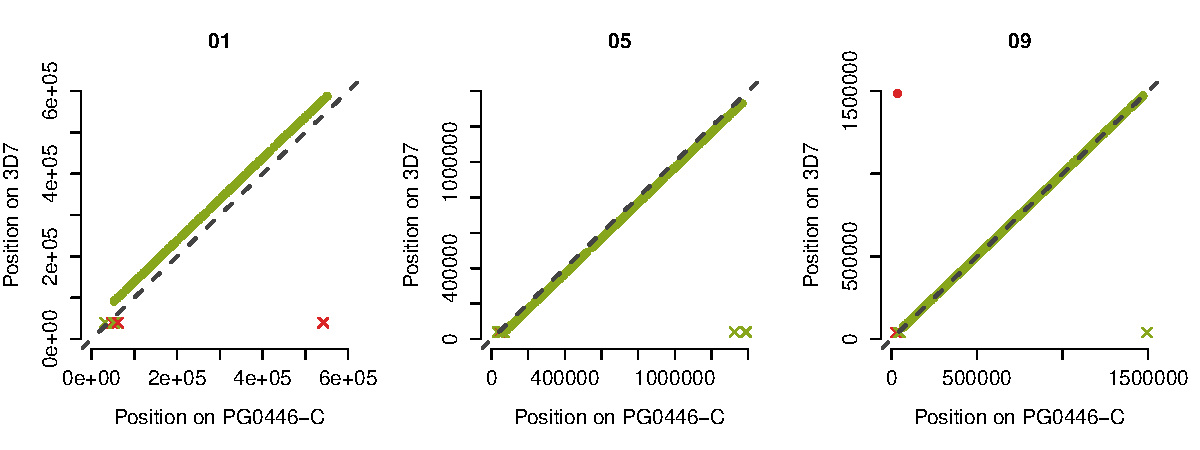
\includegraphics[width=\textwidth]{twochrs-1}
  \caption{Placement and orientation of exons from the reference assembly mapped to the PG0446-C assembly.  Chromosomes $1$, $5$, and $9$ shown.}
  \label{fig:loadGff}
\end{figure}

We verified sample identity by slicing the PacBio assembly into $1,000$ bp tiles (non-overlapping), aligning each tile to the 3D7 reference genome using \texttt{bwa mem}, and genotyping sites found to be variant in the MalariaGen 803xGB4 callset using the Genome Analysis Toolkit module, \texttt{UnifiedGenotyper} (specifying the genotype likelihood model to "SNP", ploidy to $1$, genotyping mode to "GENOTYPE\_GIVEN\_ALLELES", assuming default base quality scores should be $Q30$, and providing the 803xGB4 alleles from MalariaGen)\footnote{This procedure, while admittedly a bit indirect, provides vastly better results than genotyping the PacBio reads directly.  The assembly contains far fewer errors than the reads, even after error correction.  It is also much more straightforward than processing the MUMmer variant output, which uses a different file format to VCF, making comparisons cumbersome.}.  Chromosome $14$ is shown in Figure \ref{fig:showHaps}.  Note that while the PacBio sample's crossover pattern does appear to match that of PG0446-C, samples PG0445-C, PG0453-C, and PG0457-C also share the same pattern.  This common pattern is observed for these samples on all chromosomes.  These samples are almost certainly clones of one another.

\begin{figure}[h!]
  \centering
    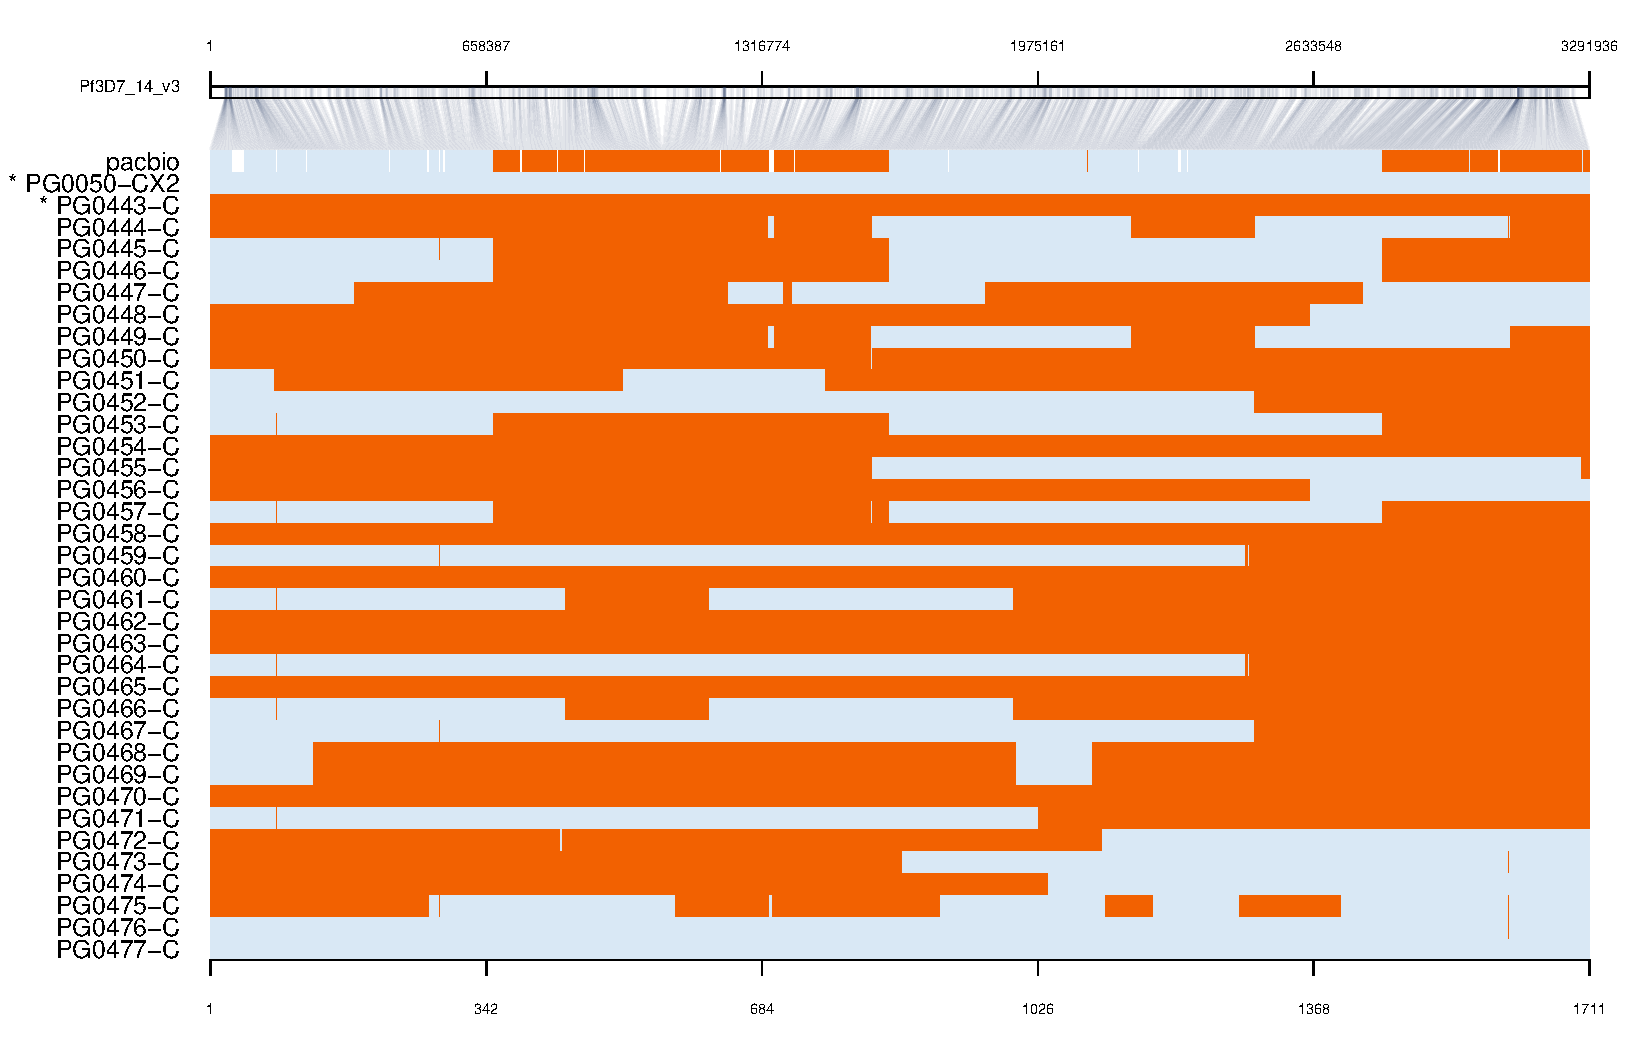
\includegraphics[width=\textwidth]{showHaps-14}
  \caption{Haplotype mosaic for chromosome $14$ in the 803xGB4 cross dataset.  Parental samples are identified with asterisks.  For remaining samples, alleles are color-coded according to the parent from which they are apparently inherited - orange for mother (PG0443-C, the 803 isolate), blue for father (PG0050-CX2, the GB4 isolate).  Missing data (sites where no genotype could be ascertained) are shown in white.  Bottom axis represents variant number.  Top axis represents variant position along the length of the chromosome.}
  \label{fig:showHaps}
\end{figure}

\section{Comparison to validation isolate}

\subsection{Verification of novel kmers}

As we have demonstrated that the PacBio assembly of the validation isolate is high-quality, novelty found in the Illumina dataset for the same sample can be verified by examining the PacBio isolate.  At the filtration levels of "all", "confident", and "trusted", initial processing of the Illumina data for 803xGB4 sample PG0446-C was found to have $28,904$; $17,069$; and $8,197$ novel kmers, respectively.  The PacBio assembly of the same sample recapitulates only $1,639$; $802$; and $48$ novel kmers, respectively.  The discrepancies can be largely attributed to three (not necessarily independent) factors: an over-aggressive lower threshold for coverage, no upper threshold, and significant data contamination.

The first two points regarding coverage can be observed in Figure \ref{fig:covdists}a-c.  The leftmost panel shows a clear valley between the left end of the distribution (presumably sequencing errors, as they are so rarely observed in the dataset) and the first local maximum (likely real data).  In the middle panel, kmer coverage in PG0446-C decays more smoothly, and it is far less obvious as to where the lower threshold should be placed\footnote{It is worth mentioning that the PG0446-C sample, sequenced on more modern Illumina HiSeq 2000 platforms, likely enjoys a much lower sequencing error rate than the Illumina GAII used for PG0055-C, which contributes to our difficulty in automatically finding a reasonable coverage threshold.}.  In the rightmost panel, all novel kmers are shown, conditional to being present or absent in the PacBio assembly of the same sample.  Our automatically calulated threshold is clearly set too high, as it is slicing through the middle of the coverage distribution for novel kmers recapitulated by the PacBio dataset.

Furthermore, the rightmost panel shows a number of coverage outliers in the set of novel kmers that are not present in the PacBio dataset.  While their source is not immediately apparent, it is clear they have a large contribution to the set of novel kmers we examine; $1,057$ kmers present in the Illumina dataset but absent in the PacBio dataset were found to be high coverage outliers.

\begin{figure}[h!]
  \centering
    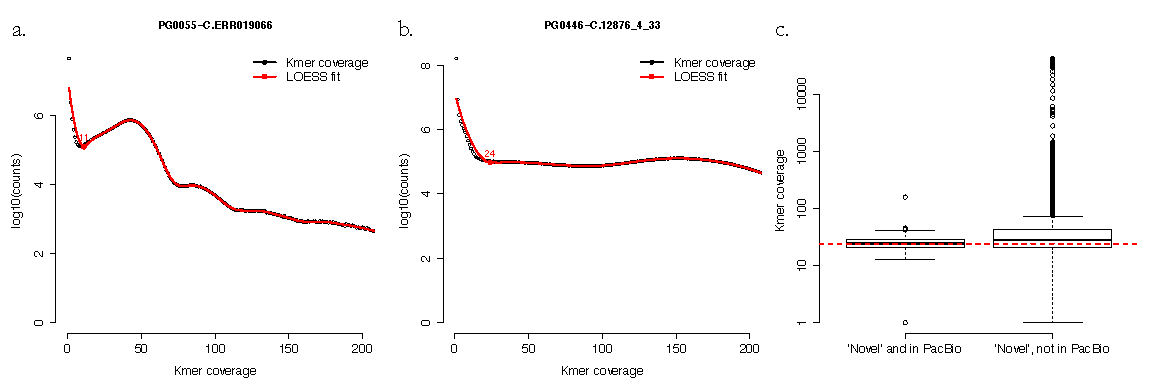
\includegraphics[width=\textwidth]{covdists}
  \caption{a. Kmer coverage in a 3D7xHB3 sample, with calculated lower threshold shown in red.  b. Kmer coverage in the 803xGB4 sample, PG0446-C, with calculated lower threshold shown in red.  c. Kmer coverage distributions for all novel kmers in PG0446-C, conditional on the kmer being present or absent in the PacBio assembly.  Calculated lower threshold from panel b shown in red.}
  \label{fig:covdists}
\end{figure}

We investigated other potentially erroneous novel kmers: putative novel kmers absent from the PacBio assembly and with coverage between $10x$ and $74x$.  We discovered many of these novel kmers exist in branches that either never connect with the graphs of the parents (we refer to these as "orphan" branches, Figure \ref{fig:orphans}a), or connect suspiciously amidst a number of putatively novel kmers rejected by the contamination checks (we refer to these as "bushy-tailed" branches, Figure \ref{fig:orphans}b).  Both appear to be symptoms of unrecognized contamination, owing to the fact that the BLAST database is not (and can never be) complete.  In attempting to remove any contribution to the graphs from non-target sources, it is insufficient to discard only the kmers that appear in the BLAST database.  Sequencing centers will always be sequencing new organisms, and the contents of the BLAST database will necessarily lag behind.  Discarding orphan branches is straightforward, but incompletely treats the problem; the bushy-tailed branches erroneously connect with the parental graphs and must be removed as well.

Finally, we discovered a substantial source of erroneous novel kmers stemming from "overcleaning", an issue wherein some kmers representing true genomic sequence are mistaken for sequencing error and removed from the graph via the assembler's error-cleaning or error-correcting process.  When this occurs in the parents but not the child (often due to coverage fluctuations), a kmer can appear to be "novel".  To mitigate this issue, we inspect the child's cleaned graph and the parents' dirty graphs.  However, a region of low coverage can also be flanked by regions of \textit{no} coverage; there are many kmers that are likely present in the parental genomes, but unobserved by chance.

\begin{figure}[h!]
  \centering
    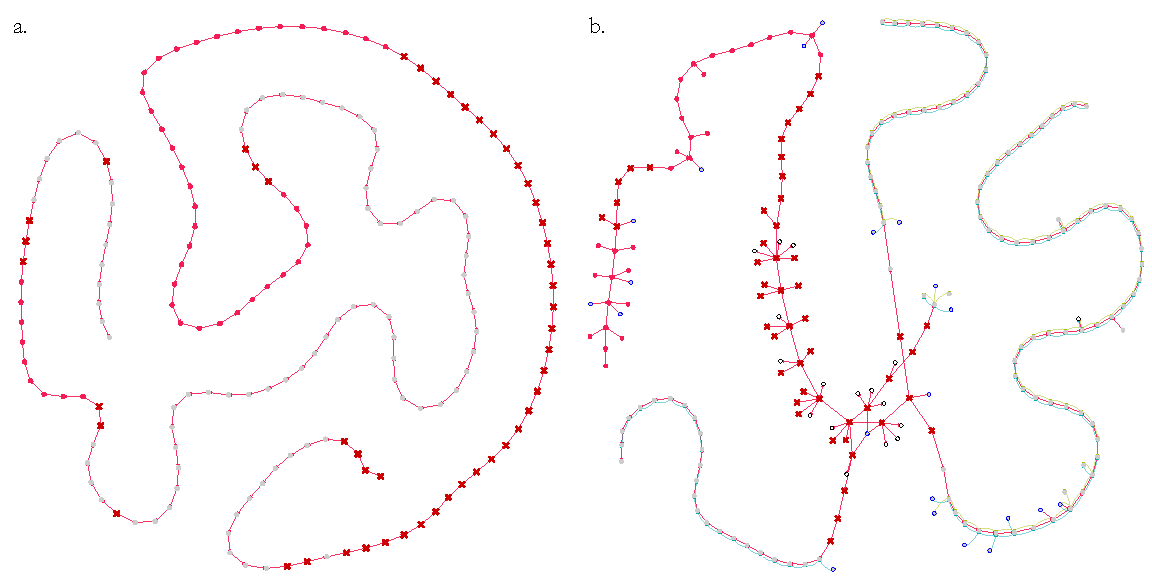
\includegraphics[width=\textwidth]{orphans}
  \caption{Local subgraphs in the Illumina data for PG0446-C near novel kmers that are absent in the corresponding PacBio assembly.  Red circles denote "trusted" novel kmers (those that passed our initial coverage and contamination checks).  Red crosses indicate "untrusted" novel kmers (those that passed our initial coverage check but failed the contamination check).  a. An "orphan" branch: a series of novel kmers not connected to the parental graphs.  b. A "bushy-tailed" branch: a series of novel kmers that appear to connect to everything, including the parental graphs, by chance.}
  \label{fig:orphans}
\end{figure}

To resolve these issues, we implemented a filtering solution for novel kmers in four parts.  First, we implemented a manual procedure for specifying coverage limits, selecting a lower limit of $10x$ and an upper limit of $74x$.  Next, we implemented software to explore the trio graph starting at confident novel kmers rejected by the contamination filter using our condition-limited depth first search software.  Explored branches containing novel kmers that are on the same branch as rejected kmers are similarly tagged for rejection.  Third, we explore the trio graph starting with remaining confident novel kmers.  If the explored subgraph does not connect with the parental graphs in any way, the kmers in the branch are marked for rejection and removed from further consideration.  Finally, we examine contigs with "overcleaned" novel kmers (i.e. any kmer that would be considered novel by comparing to the cleaned parental graphs, but is subsequently denied this label after examining the dirty parental graphs).  Novel kmers found on the same contig are considered tainted and removed from consideration.  Any putatively novel kmer surviving this battery of tests is considered "filtered".

The results of our novel kmer filtering are shown in Figure \ref{fig:novelfilter}.  $95$ kmers survive our battery of filters to be considered truly novel sequence in the genome of the PG0446-C child.  We called DNMs in the Illumina data using our graph-based calling software and discovered three events: two SNPs ($47$ kmers each) and a single kmer occurring in a repetitive region of a telomere; the precise nature of this single-kmer event is not clear.  The PacBio dataset contains $51$ novel kmers, $48$ of which overlap our calls (one SNP and the unknown event).  The other $47$ kmers from the second SNP are not present in the PacBio assembly.  However, manual inspection reveals this SNP to be polymorphic, possibly indicating a \textit{de novo} mutation that has occurred in the sample during mitosis that has not yet reached fixation in the sequenced population of cells.  It is likely that the event (shown in Figure \ref{fig:fpcomp}) is a true variant, absent in the PacBio assembly as the Celera assembler is forced to make a choice between which allele to retain in the haploid assembly.  The presence of the alternate allele in the uncorrected PacBio reads strongly suggests this is event is real and its absence from the assembly is an artifact of the assembler's bubble-popping procedure.  The remaining $3$ kmers from the PacBio dataset are not called in the Illumina data as they are low coverage (all at $1x$ coverage, all low complexity sequence, possibly representing recurrent sequencing errors in both the PacBio and Illumina data).

\begin{figure}[h!]
  \centering
    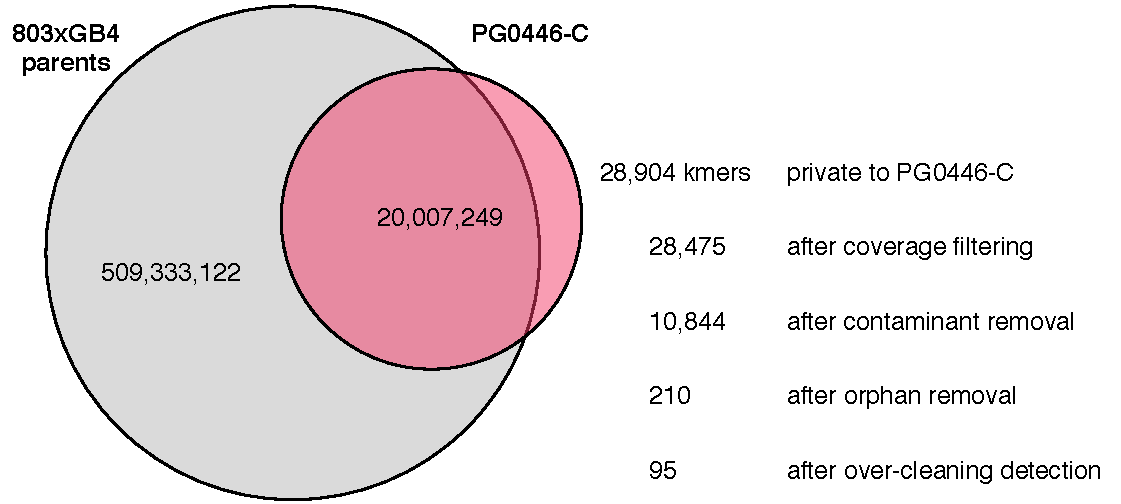
\includegraphics[width=\textwidth]{novelfilter}
  \caption{The results of filtering kmers private to the PG0446-C child }
  \label{fig:novelfilter}
\end{figure}

Based on the kmer recovery results listed above, our sensitivity to novel kmers is between $94\%$ and $100\%$ (depending on whether the $3$ missed kmers are considered truly novel kmers or sequencing errors), and specificity is greater than $99\%$.  Both SNPs and the unknown third event are recovered successfully.  The two SNPs are shown in Figures \ref{fig:pacbiohomsnpigv} (A to G, $13:2,032,381$) and \ref{fig:pacbiohetsnpigv} (C to T, $14:1,396,035$, a non-synonymous substitution resulting in a T to I amino acid change).  Figure \ref{fig:pacbiounknownigv} shows the third, unknown event.

\begin{sidewaysfigure}[h!]
  \centering
    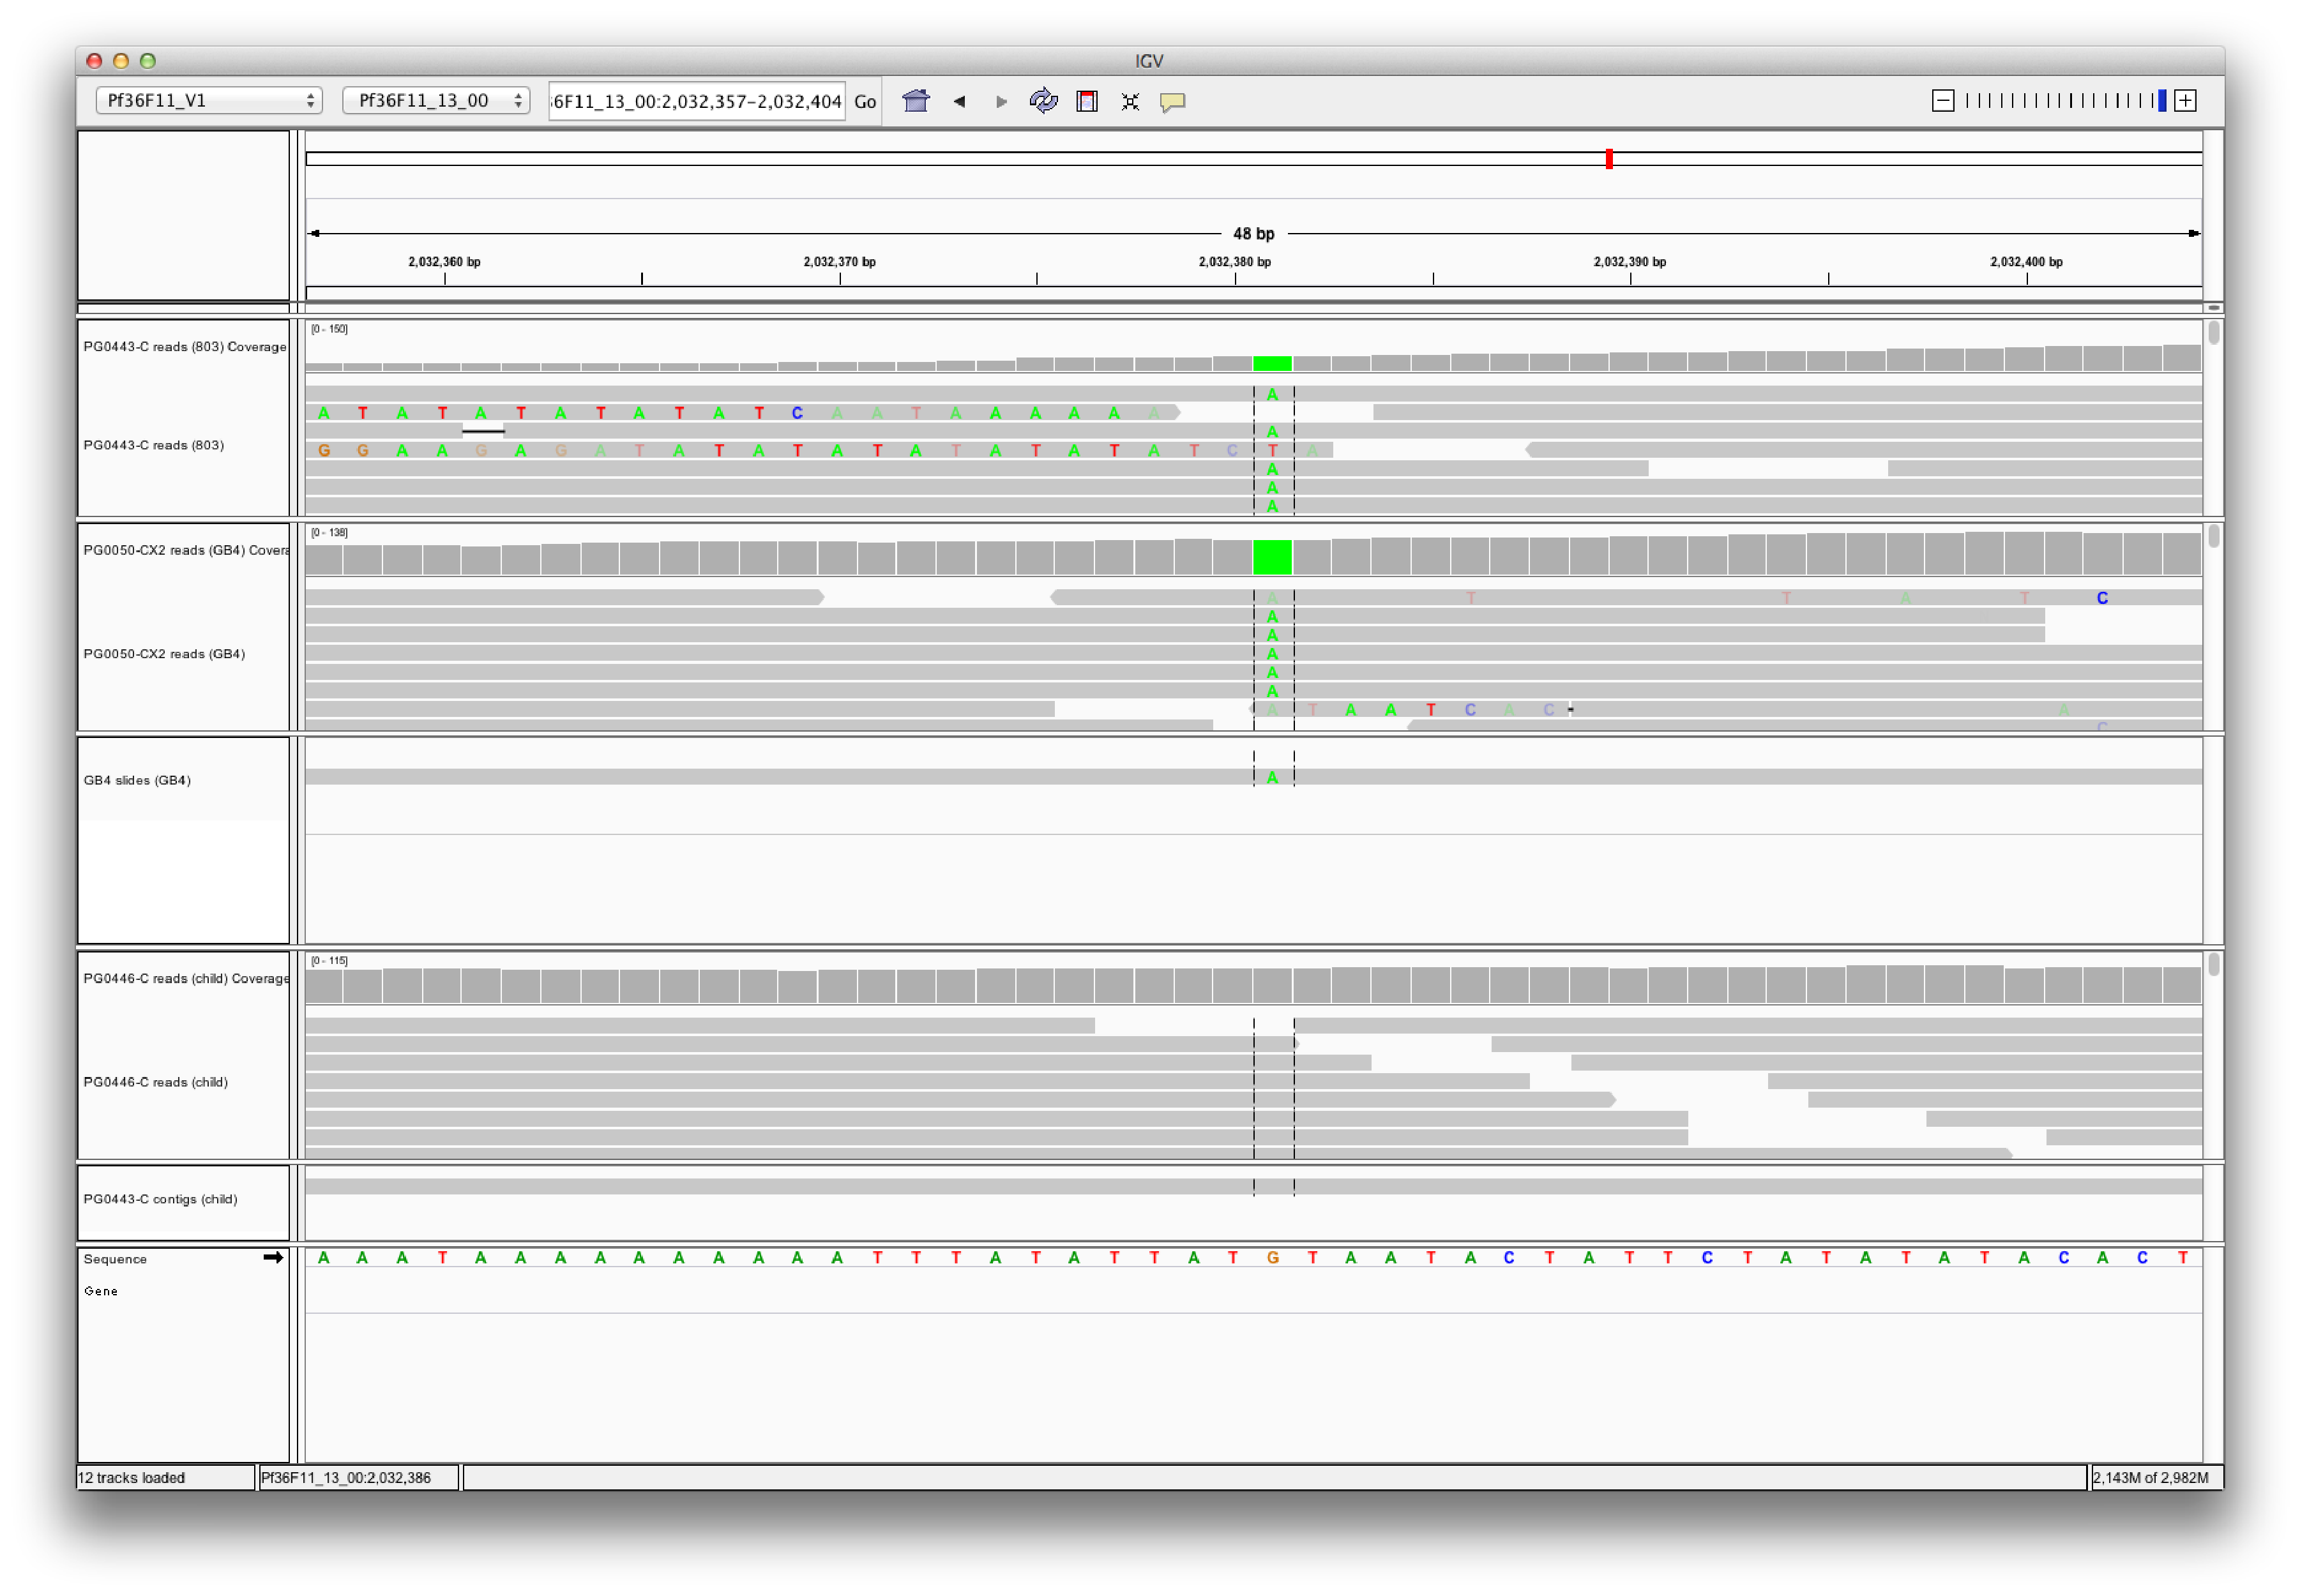
\includegraphics[width=\textwidth]{pacbiohomsnpigv}
  \caption{IGV screenshot of an A to G SNP, showing reads and assembly information for the trio, aligned to the PacBio PG0446-C assembly.  Top panel: 803.  Middle two: GB4 reads and PacBio assembly (sliced to facilitate alignment).  Lower two: PG0446-C reads and contig containing the variant in question from the a. panel.}
  \label{fig:pacbiohomsnpigv}
\end{sidewaysfigure}

\begin{sidewaysfigure}[h!]
  \centering
    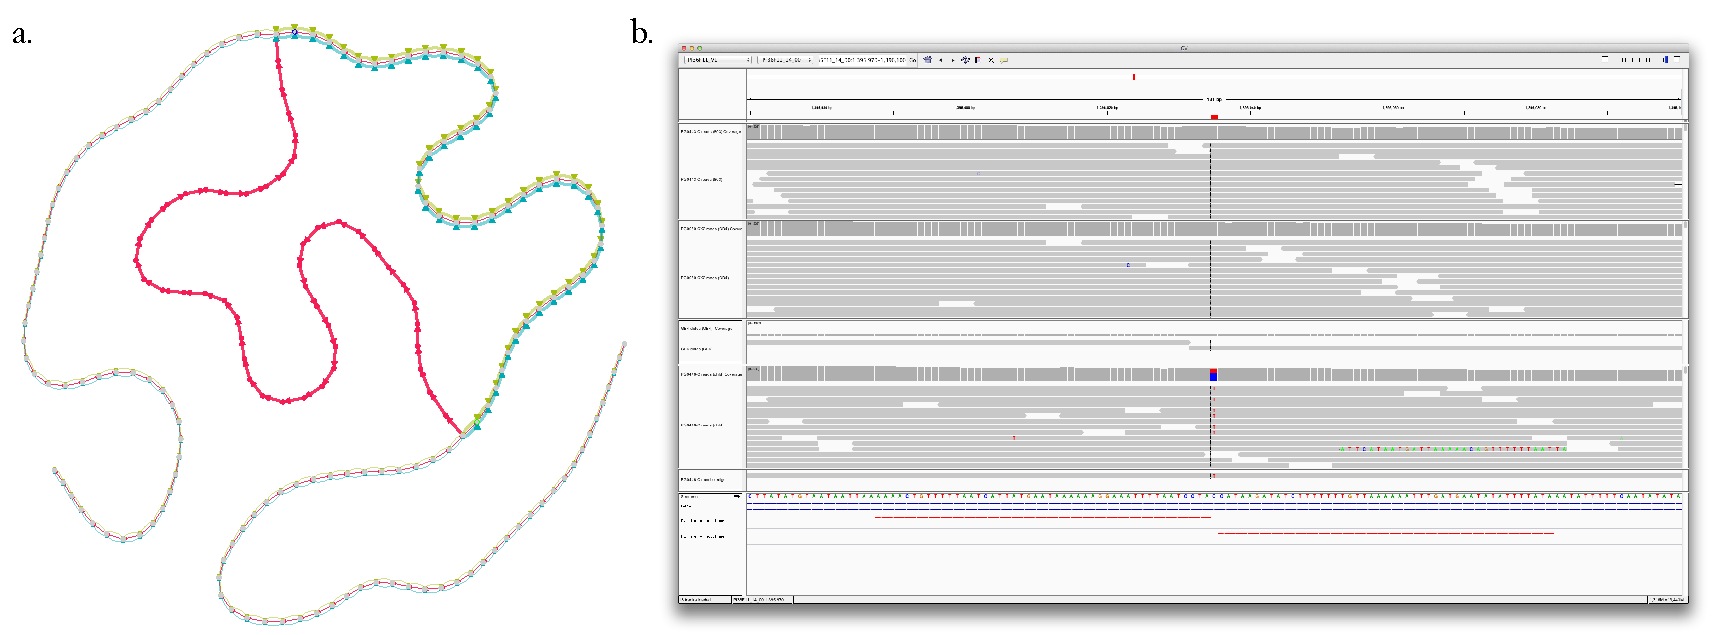
\includegraphics[width=\textwidth]{fpcomp}
  \caption{A C to T SNP that has likely not reached fixation in the sequenced population of ostensibly clonal parasites.  a. Local subgraph at the site, wherein the child's graph contains paths that traverse the series of novel kmers as well as the parental kmers, indicating polymorphic status.  b. IGV screenshot of the site showing reads and assembly information for the trio, aligned to the 3D7 reference genome.  Top panel: positions of the called variants in the reference-basde analysis.  Second panel: PG0443-C (803).  Third: PG0050-CX2 (GB4).  Fourth: PG0446-C (child).  Fifth: Uncorrected PacBio reads from PG0446-C.  Bottom: gene model track from PlasmoDB $9.0$.  Stacked barplots above tracks indicate the proportion of reads supporting each allele.}
  \label{fig:pacbiohetsnpigv}
\end{sidewaysfigure}

\begin{sidewaysfigure}[h!]
  \centering
    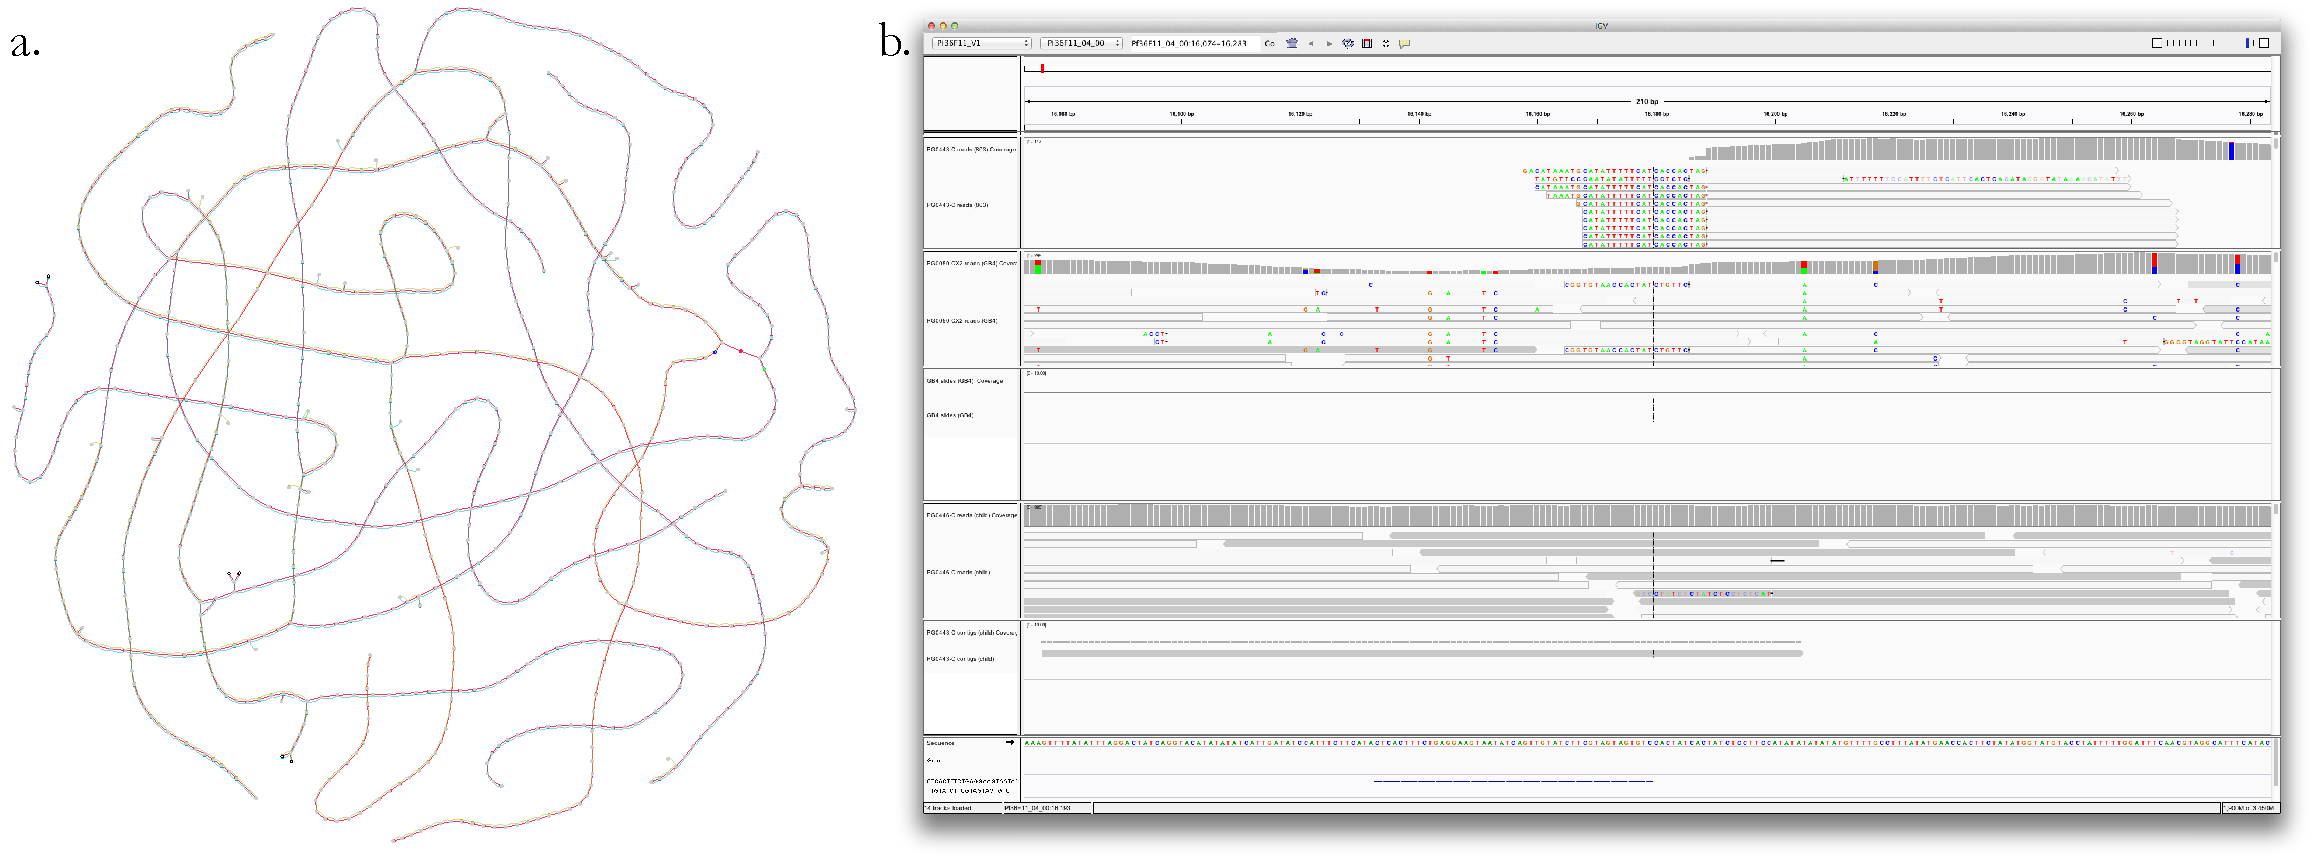
\includegraphics[width=\textwidth]{weirdsinglenovelkmercomp}
  \caption{A strange event involving a single novel kmer.  a. Local subgraph at the site; the novel kmer in question is depicted as a filled red vertex in the right side of the image.  b. IGV screenshot of the site showing reads and assembly information for the trio, aligned to the PacBio PG0446-C assembly.}
  \label{fig:weirdsinglenovelkmercomp}
\end{sidewaysfigure}

\subsection{Comparison to reference-based analysis}

We sought to determine our relative ability to detect DNMs accurately compared to that of the reference-based analysis.  As the release version of the MalariaGen callset purposefully excluded \textit{de novo} mutations (attempting to minimize Mendelian error rates to ensure high confidence in the inherited variation callset), we set about we processing the Illumina data from the PG0446-C trio (PG0443-C (803), PG0050-CX2 (GB4), and PG0446-C) ourselves.  Reads were aligned with \texttt{bwa mem} to the 3D7 reference genome, release $9.0$ from PlasmoDB.  PCR duplicates were marked with the \texttt{MarkDuplicates} program from the Picard suite; these marked reads were subsequently ignored in downstream processing.  A list of genomic regions with reads appearing to span indels were discovered using the GATK's \texttt{RealignerTargetCreator} module (supplemented by MalariaGen's 803xGB4 calls as additional candidate regions to consider).  We subsequently ran the GATK's \texttt{IndelRealigner} to perform the local realignments on these candidate regions.  We recalibrated base quality scores using the GATK's \texttt{BaseRecalibrator} tool, once again supplying the MalariaGen calls as sites to ignore when computing the data error model.  Variants were called across the PG0443-C, PG0050-CX2, and PG0446-C samples simultaneously using the GATK's \texttt{HaplotypeCaller} module, which performs local \textit{de novo} assembly to determine the haplotype sequence at so-called "active sites", windows of the genome detected to harbor some sort of variation.  For each approach, we specified a ploidy of $1$.  SNPs and indels were filtered separately using the GATK's \texttt{VariantRecalibrator} tool, supplying the MalariaGen calls as training data.  We set the desired truth sensitivity to $99\%$ (i.e. requesting that the recalibration tool learn filter thresholds such that at least $99\%$ of the MalariaGen calls were recapitulated).  Finally, we isolated putative DNMs by selecting sites confidently called in all three samples, where the genotype of the child differed from that of mother and father, requiring confident genotypes in all three samples (i.e. $GQ > 90$), and sufficient allele depth in all three samples (i.e. $DP > 20$).

Callset metrics are presented in Table \ref{tbl:gatkmetrics}.  Note that while MalariaGen chose to include calls only in the so-called "core" region of the genome (comprising $20.7$ Mbp of sequence), we have included the accessory genome in our callset as well (the remaining $2.5$ Mbp of genomic sequence spanning telomeric, subtelomeric, pericentromeric, and other hypervariable loci).  For a fairer comparison, we have partitioned the calls into the core and accessory regions.  Furthermore, in addition to the monomorphic sites one expects to see in a haploid genome for a \textit{de novo} variant that occurs during meiosis or in one of the gametocytes, the trio contains thousands of polymorphic sites ($23,004$ sites where the reference allele and alternate allele have non-zero coverage, $4,364$ with reference and alternate allele coverage greater than $10x$).  Both the accessory genome and polymorphic sites are easily removed.  However, given that our graph-based approach is theoretically able to access the accessory genome and that we saw at least one polymorphic site in our graph-based \textit{de novo} mutation callset, we chose not to exclude these sites at this stage.

\begin{table}[]
\centering
\caption{Callset metrics in the PG0446-C sample of the trio}
\label{tbl:gatkmetrics}
\begin{tabular}{@{}rrrrrr@{}}
\toprule
\multicolumn{1}{l}{}           & All      & In MalariaGen & Not in MalariaGen & Core     & Accessory \\
\midrule
\multicolumn{1}{l}{SNPs}       &          &               &                   &          &           \\
\textit{all}                   & $28,613$ & $5,742$       & $22,871$          & $13,700$ & $14,913$  \\
\textit{de novo}               & $128$    & $0$           & $128$             & $7$      & $121$     \\
\multicolumn{1}{l}{Insertions} &          &               &                   &          &           \\
\textit{all}                   & $15,163$ & $4,543$       & $10,620$          & $12,540$ & $2,623$   \\
\textit{de novo}               & $38$     & $0$           & $38$              & $8$      & $30$      \\
\multicolumn{1}{l}{Deletions}  &          &               &                   &          &           \\
\textit{all}                   & $17,762$ & $5,160$       & $12,602$          & $15,123$ & $2,639$   \\
\textit{de novo}               & $30$     & $0$           & $25$              & $5$      & $25$      \\
\multicolumn{1}{l}{MNPs}       &          &               &                   &          &           \\
\textit{all}                   & $144$    & $0$           & $144$             & $65$     & $79$      \\
\textit{de novo}               & $0$      & $0$           & $0$               & $0$      & $0$       \\
\bottomrule
\end{tabular}
\end{table}

We identified $196$ potential \textit{de novo} variants in the PG0443-C sample using the reference-based \texttt{HaplotypeCaller} approach and the filters described above.  This is two orders of magnitude greater than the number of DNMs we found in the PacBio data.  As expected, much of this putative variation appears in the accessory compartments of the genome, owing to the massive divergence between the reference and sampled haplotypes.  However, even when we restrict our analysis to the core genome, we still find an order of magnitude more events than we expect.

We sought to establish the veracity of any of these putative \textit{de novo} events.  Assuming the child's underlying haplotype is the reference haplotype plus the variants discovered in that sample, we expected to find kmers spanning the DNMs to be present in the PacBio assembly, present in the clean graph of the child, and absent in the dirty graphs of the parents.  Revisiting Algorithm \ref{alg:all_subsets} from Chapter \ref{ch:motivation}, we combinatorically generated kmers spanning all \textit{de novo} variants and any nearby variants (including variants that were filtered out) that would affect the local haplotype.  $30,360$ such kmers were generated, $3,740$ of which are present in our PacBio draft reference for the child.  $3,547$ ($\approx 95\%$) of these kmers are present in the Illumina data for the child as well.  $3,500$ of these are present in the dirty graphs of the parents, suggesting that all associated events ($195/196$) are false positives.

The remaining $47$ kmers represent a single SNP: the clearly homozygous SNP on chromosome $13$ discussed in the previous section.  This is the only event recapitulated between the PacBio dataset and these calls.  However, we note that in selecting our coverage thresholds, we benefitted from prior knowledge.  The coverage in the 803 parent is approximately $30x$, while coverage in the GB4 parent and the child are in excess of $60x$; our depth filtering threshold was specifically chosen to recover this validated variant.  The SNP is shown in Figure \ref{fig:homlowcov}; the PG0443-C (803) panel shows the drop in coverage in the downstream intergenic region beyond PF3D7\_1350600.  In this region, sequence complexity drops sharply, dominated by runs of As and Ts.  Sequencing error may be accumulating in reads sampled from this region such that they fail to align back, thus contributing to the coverage falloff.  Raising the coverage threshold would of course remove more false-positives, but there is no \textit{a priori} reason to choose a threshold of $20x$ versus $30x$ (especially when average coverage in the 803xGB4 samples is around $200x \pm 100x$).

The polymorphic variant on chromosome $14$ is not present in the reference-based callset, owing to the fact that we instructed \texttt{HaplotypeCaller} to assume a ploidy of $1$.  If we genotype this site alone without the ploidy specification, we can recover the event.  However, removing the ploidy specification does not mean allowing any ratio of reference to non-reference alleles at a putative variant site.  Instead, the software simply defaults to a ploidy of $2$, which is not necessarily a correct assumption to make for our data.  The ploidy setting merely enables the caller to adjust its allele balance expectations, and revising it upwards increases the chance that the caller will accept sequencing error as variation.  Thus, removing the ploidy setting would necessarily increase the false-positive rate as well.

We visually inspected the alignments spanning the false \textit{de novo} events using IGV.  Many of these sites were seemingly polymorphic as well, in close proximity to one another, and in known high-diversity regions of the genome.  Figure \ref{fig:lotsosnps} depicts one such example of false-positives on chromosome $2$.  It is possible to begin adding heuristic filters to remove these events (e.g. rejecting events on allele balance, inter-marker distance, and the genomic compartment in which they are discovered).  However, there are two very good reasons not to do so.

First, consider the underlying cause of these artifacts.  The myriad inconsistencies between the Illumina reads for PG0446-C, the PacBio reads for the same sample, and the presence of many mapping quality $0$ reads, strongly suggests misalignment.  The true haplotype from which these reads are sampled are clearly not in the reference genome, but are similar enough that many reads map anyway, and the precise placement is a function of read length and repetitiveness of the sampled haplotype.  When we align reads from this region in the child to the PacBio reference for the child, we find that most map to chromosome $1$, not chromosome $2$.  Filters can only accomplish one thing: reject potential false-positives.  However, filters can do nothing to address the root issue: the reads were sampled from one region of the child's genome and aligned to a sample too genomically divergent in these loci to serve as a useful platform for comparison.  Application of such filters would necessarily require sacrificing any ability to say something meaningful about enormous diverse regions of the genome.

Second, consider what these variants in a haploid genome must represent: \textit{de novo} mutations that have occurred while the parasites have been in culture and have not reached fixation in the sample.  These events necessarily must have occurred during mitosis, as mutations incurred during meiosis or present in the gametocytes would appear in every read spanning the site.  Filtering any events based on allele balance would necessarily mean discarding every potential mitotic \textit{de novo} mutation\footnote{In a haploid genome, every true variant presenting as seemingly polymorphic must be a mitotic event, but as some mutations could have reached fixation in the sample, not every mitotic event will necessarily present as polymorphic.}.

\begin{sidewaysfigure}[h!]
  \centering
    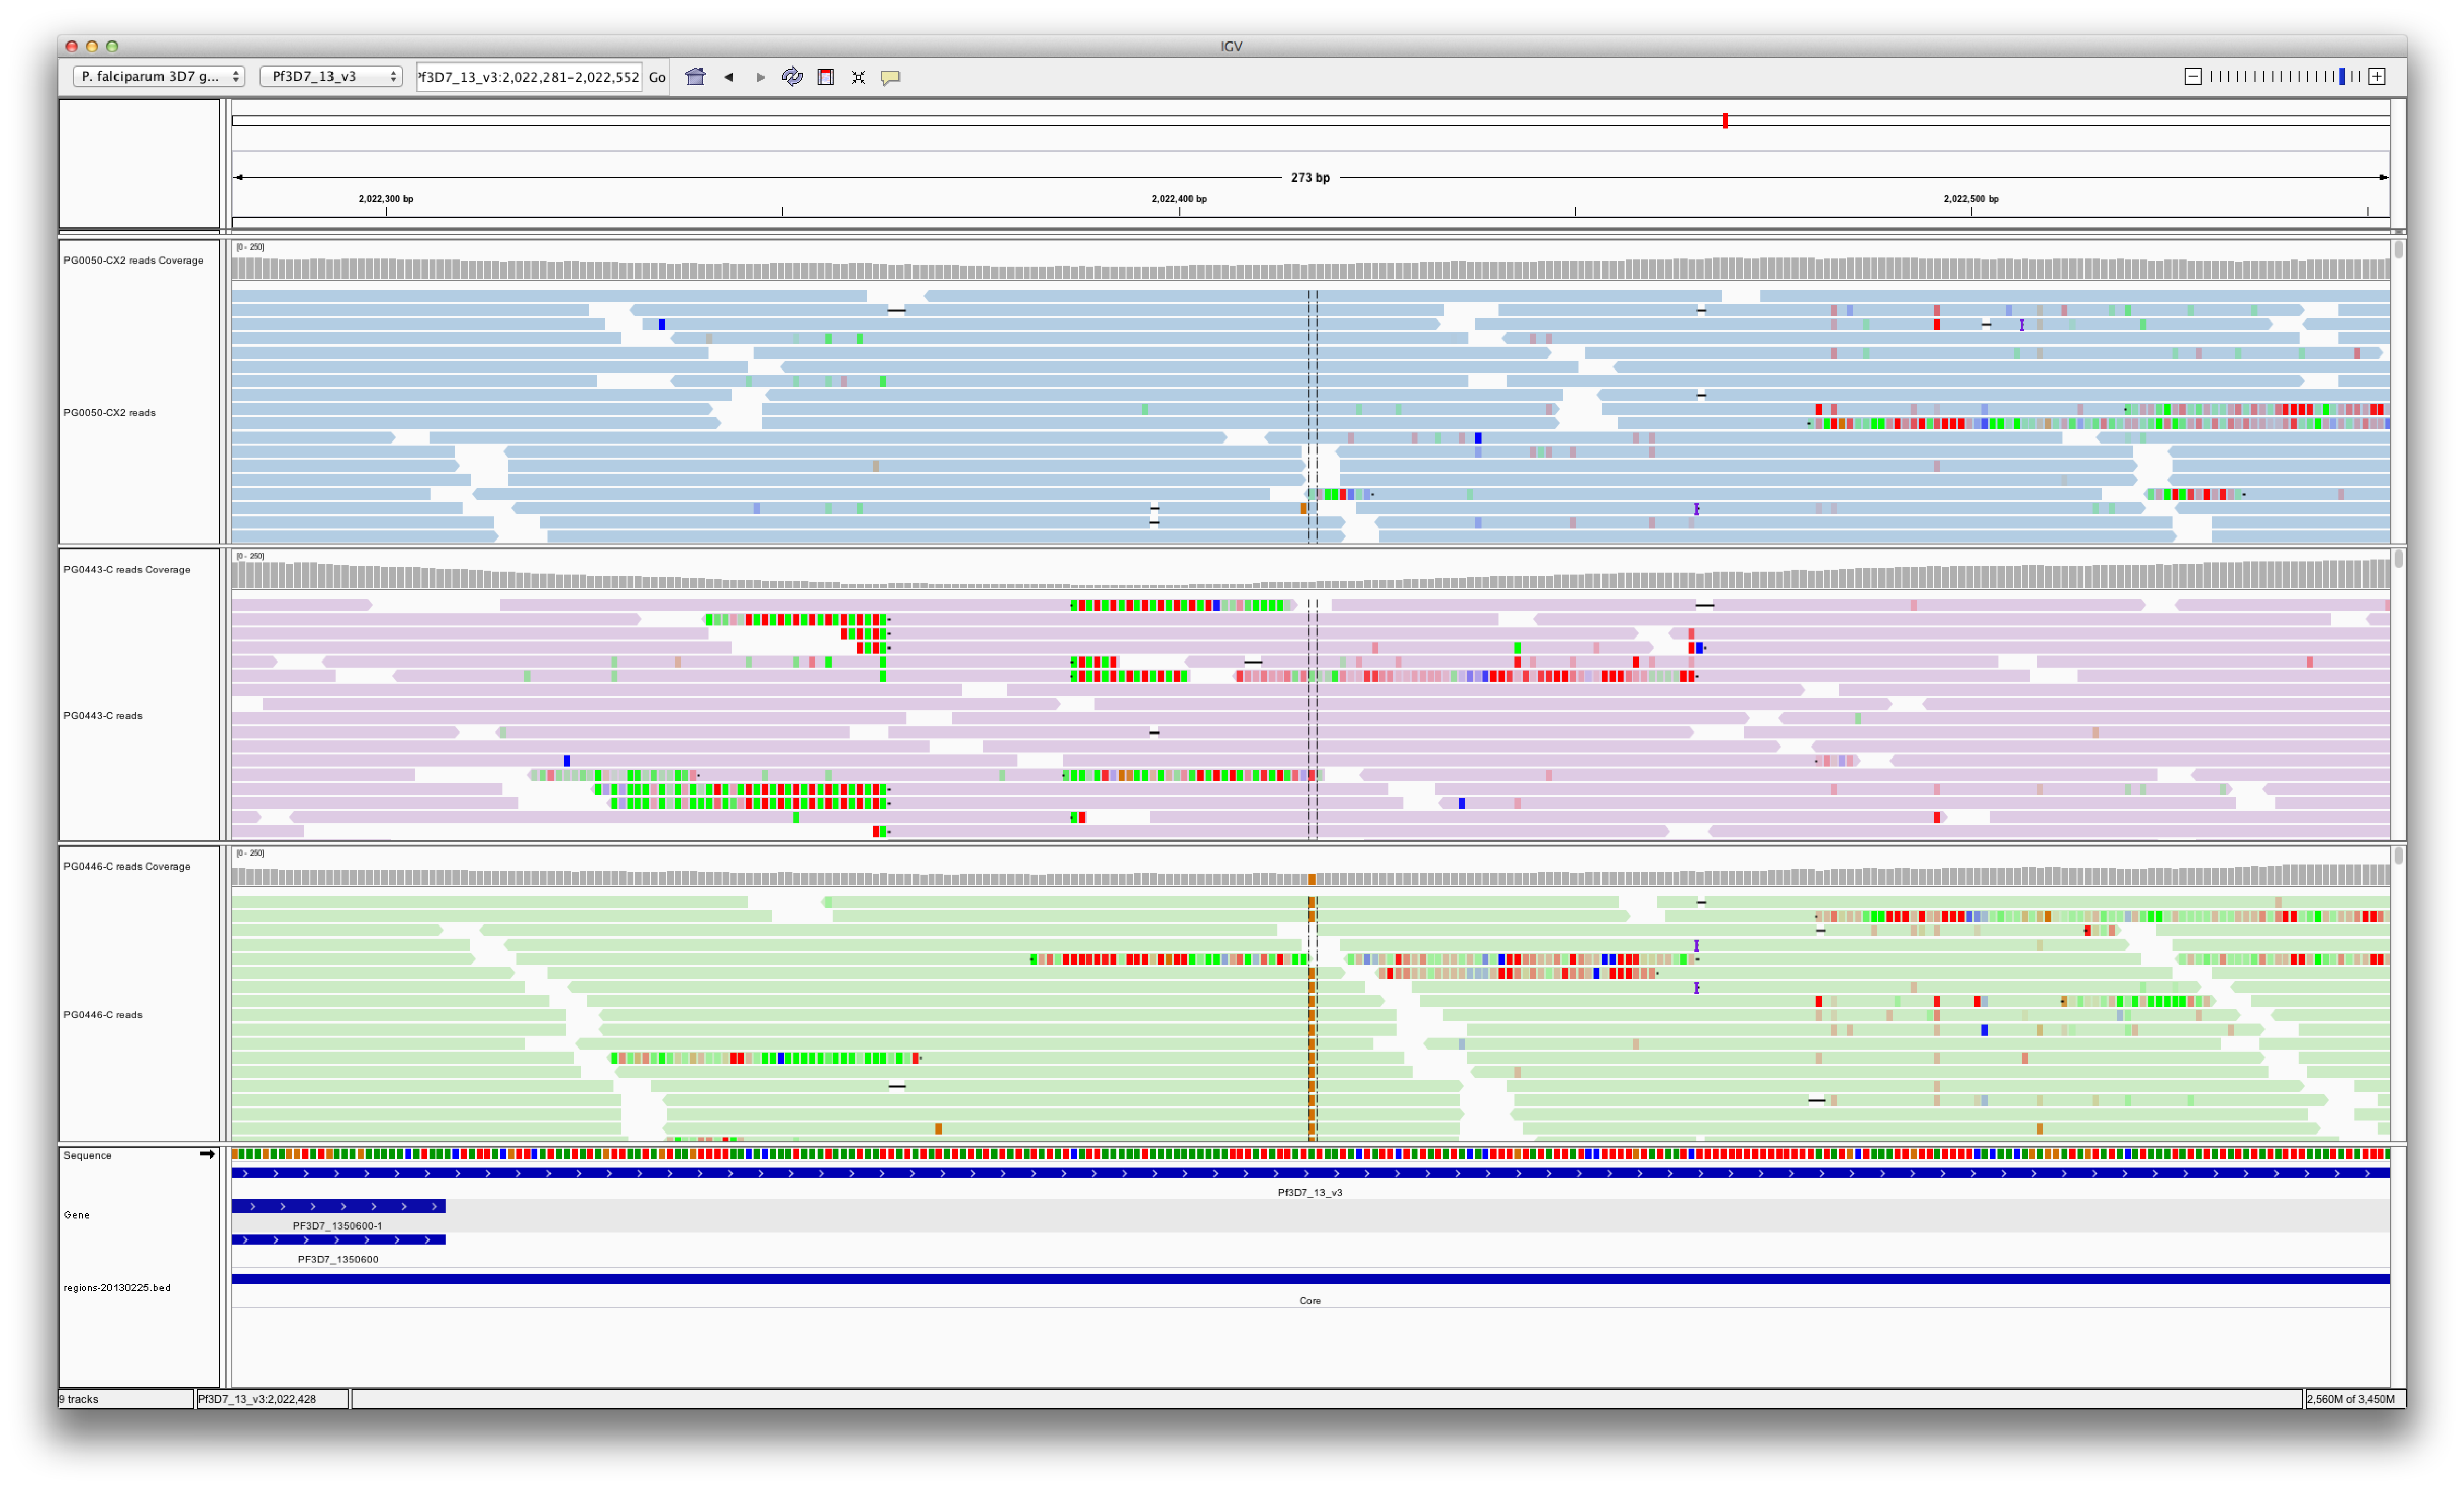
\includegraphics[width=\textwidth]{homlowcov}
  \caption{A validated \textit{de novo} SNP, recovered in the child amidst a great deal of sequencing error.  Top panel: PG0443-C (803).  Middle panel: PG0050-CX2 (GB4).  Lower panel: PG0446-C (child).}
  \label{fig:homlowcov}
\end{sidewaysfigure}

\begin{sidewaysfigure}[h!]
  \centering
    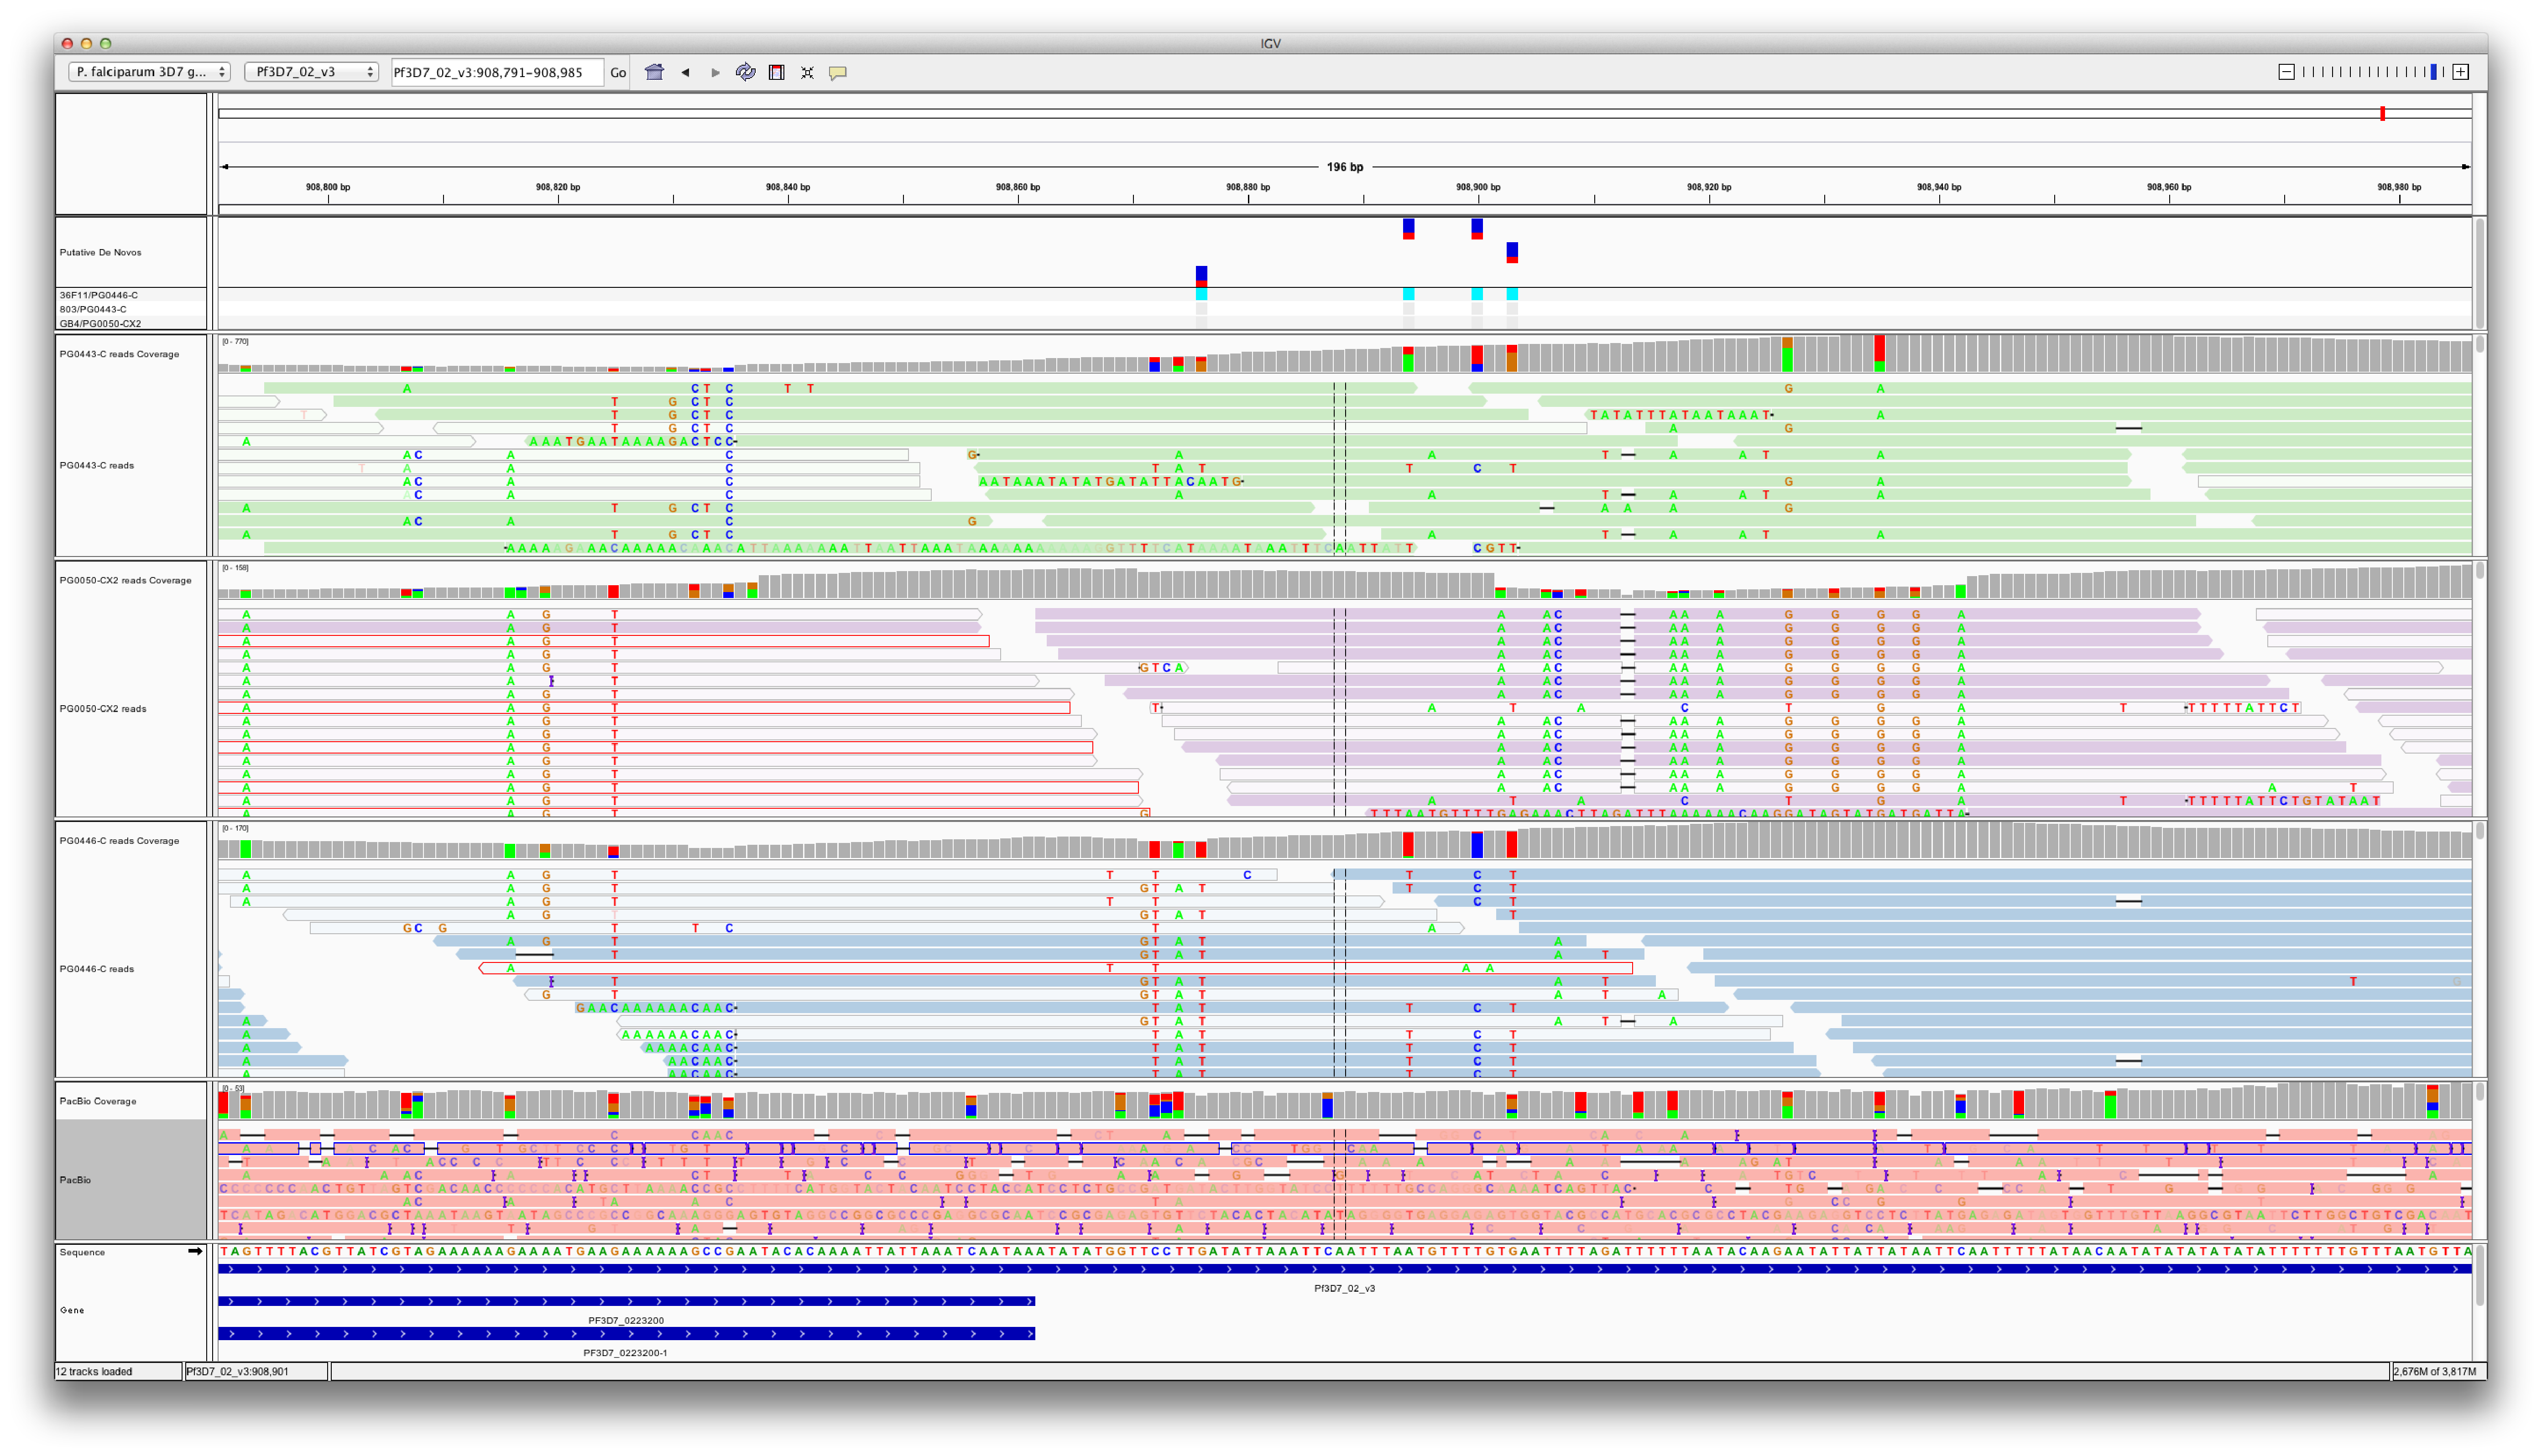
\includegraphics[width=\textwidth]{lotsosnps}
  \caption{False-positive \textit{de novo} variants in the 3' subtelomeric region of chromosome $2$.  Top panel: positions of the called variants in the reference-based analysis.  Second panel: PG0443-C (803).  Third: PG0050-CX2 (GB4).  Fourth: PG0446-C (child).  Fifth: Uncorrected PacBio reads from PG0446-C.  Bottom: gene model track from PlasmoDB $9.0$.  Stacked barplots above tracks indicate the proportion of reads supporting each allele.  Reads with ambiguous alignments are displayed in a lighter shade.}
  \label{fig:lotsosnps}
\end{sidewaysfigure}

\section{\textit{De novo} mutations in a single 3D7xHB3 sample}

\subsection{List of mutations}

A single validation sample is limited in its ability to inform us on the efficacy of the graphical variant calling approach, particularly as it apparently lacks an NAHR or other complex event for us to inspect.  We thus turned our attention to a single sample from the $3D7xHB3$ cross: PG0063-C.  This sample is known to harbor an NAHR event between two \textit{var} genes: $PF3D7\_0100100$ (situated in the 5' subtelomere of chromosome $1$), and $PF3D7\_0223500$ (the 3' subtelomere of chromosome $2$).  Their validated presence in PG0063-C makes this sample a particularly useful test sample for examination.

Applying our novel kmer identification software (and the new filters described above), we identified $314$ novel kmers corresponding to $77$ putative events.  Post-calling filtration brought this list down to $7$ events, described in Table \ref{tbl:callsPG0063C}.  These events are annotated with the locus, the haplotypic background of the variant, variant type, closest gene (and the associated product), and whether the variant falls within the MalariaGen variant calling exclusion mask.  The variants can be seen in their genomic context in Figure \ref{fig:circosPG0063C}.  

\begin{landscape}
\begin{table}[]
\centering
\caption{\textit{De novo} variants in 3D7xHB3 progeny, PG0063-C}
\label{tbl:callsPG0063C}
\begin{tabular}{@{}lllllll@{}}
\toprule
       & locus                & background &  event    &  closest gene                   &  product           &  within mask  \\
\midrule
1 (a)  & 1:27,780             & 3D7        &  SNP      &  PF3D7\_0100100                 &  PfEMP1 (var)       & yes          \\
1 (b)  & 1:27,782             & 3D7        &  MNP      &  PF3D7\_0100100                 &  PfEMP1 (var)       & yes          \\
1 (c)  & 1:27,854             & 3D7        &  MNP      &  PF3D7\_0100100                 &  PfEMP1 (var)       & yes          \\
1 (d)  & 1:29,441;2:923,083   & 3D7        &  NAHR     &  PF3D7\_0100100;PF3D7\_0223500  &  PfEMP1 (var)       & yes          \\
1 (e)  & 2:923,083;8:21,877   & 3D7        &  NAHR     &  PF3D7\_0223500;PF3D7\_0800100  &  PfEMP1 (var)       & yes          \\
1 (f)  & 8:21,877;1:30,087    & 3D7        &  NAHR     &  PF3D7\_0800100;PF3D7\_0100100  &  PfEMP1 (var)       & yes          \\
1 (g)  & 2:925,756;1:27,374   & 3D7        &  unknown  &  PF3D7\_0100100;PF3D7\_0223500  &  PfEMP1 (var)       & yes          \\
1 (h)  & 2:919,850            & 3D7        &  SNP      &  PF3D7\_0223500                 &  PfEMP1 (var)       & yes          \\
2      & 2:394,194            & HB3        &  unknown  &  PF3D7\_0209600                 &  transporter        & no           \\
3      & 4:568,395            & 3D7        &  SNP      &  PF3D7\_0412700                 &  PfEMP1 (var)       & yes          \\
4      & 4:568,401            & 3D7        &  SNP      &  PF3D7\_0412700                 &  PfEMP1 (var)       & yes          \\
\bottomrule
\end{tabular}
\end{table}
\end{landscape}

\begin{figure}[h!]
  \centering
    \includegraphics[width=\textwidth]{{PG0063-C.ERR019060.circos.edr}.png}
  \caption{Circos visualization of all \textit{de novo} mutations in PG0063-C, positioned on the reference sequence (outer ring), aligned maternal assembly (middle), and aligned paternal assembly (inner).  Unplaced parental contigs are concatenated and placed in the "U" pseudochromosome.  Each parental ring is annotated with a sequence compressibility score for every $2,500$ bp shown above their ideograms, while the reference ring is annotated with mean read coverage per $2,500$ bp.  Within the reference ideogram, all reference-based variant calls made in this sample from the MalariaGen project are shown, color-coded to reflect their parentage.  Regions that were masked out of MalariaGen's variant calling process are shown as grey bars.  Variants are shown as glyphs below the parental ideograms, shape-coded for type (small circle: unknown, large circle: SNP, triangle: indel, square: MNP, diamond: NAHR event).  The color and positioning of the glyph reflects the haplotypic background upon which the event occurred.  Interchromosomal structural variation and gene-conversion events are additionally denoted as arcs linking the relevant parts of the genome.  The closest gene to the event is reported in black if the mutation falls within the gene and as grey if it falls outside the gene.}
  \label{fig:circosPG0063C}
\end{figure}

There are several noteworthy features of Table \ref{tbl:callsPG0063C} and Figure \ref{fig:circosPG0063C}.  First, we discover a variety of event types, including SNPs (depicted in the plot with large circles), indels (triangles), multi-nucleotide polymorphisms (squares), and NAHR events (diamonds).  Few events could not be typed (small circles).

Second, we are able to localize all mutational events within the parental genomes, even if the precise nature of the event could not be ascertained.  Here, we benefit from aligning the parental sequences rather than the child's sequence or short $76$ bp reads.  The parental sequences are often be longer than a read length, and should obviously match the parental genomes more closely.  This provides the alignment software more context and less variation with which to determine an appropriate home for the mutation.

Third, we are able to identify interchromosomal exchanges, including the known NAHR event between PF3D7\_0100100 on the 5' end of chromosome $1$ and PF3D7\_0223500 on the 3' end of chromosome $2$\cite{Anonymous:2013hi}.  Curiously, there is another apparent interchromosomal exchange involving these two \textit{var} genes and one on chromosomes $8$.  No such recombination is reported in the literature, and the event is supported by a very short contig aligned to chromosome $8$ ($< 50$ bp).  While it is conceivable that the NAHR machinery may switch templates to potentially involve content from a third chromosome, it is more plausible that the recombination process gave rise to a short region of low-complexity sequence that happens to occur elsewhere in the genome.

Fourth, we are able to detect mutations that occur in regions of the reference genome typically ignored in reference-based analyses.  MalariaGen delibrately excluded a number of regions from processing, including repetitive regions (often telomeric, centromeric, or pericentromeric regions) as short reads could often not be aligned in long repetitive regions with confidence.  It also excluded hypervariable regions (typically subtelomeric) as population diversity was too high to yield confident results in the reference-based analysis.  As we are comparing each sample to a parental graph rather than a reference sequence that is an undetermined number of generations removed, our graphical approach can reconstruct and localize these events.

Fifth, our calls in this sample appear overwhelmingly concentrated in or near antigenic genes ($8$/$9$).  Such a skew is unusual, especially given the fact that our algorithm is hypothesis-free and is not biased towards processing any particular region of the genome.

Sixth, the call rate is reasonably low; $9$ events in this sample total.  However, the first several events in the table appear to take place in the same \textit{var} genes.  Presumably, these events are all part of the single NAHR event.  Counted together, the revised \textit{de novo} mutation count is $4$.  Both are consistent with the expectation from the validation data that \textit{de novo} mutations should be rare.

Subtelomeric regions (and the antigenic genes contained within) are known to be high in repetitive sequence.  To visualize the potential relationship between sequence content and variant location, we examined a number of different sequence properties.  Shown in Figure \ref{fig:circosPG0063C} above each parental assembly track is one of these metrics: the sequence compression ratio.  Many of our DNM calls appear to follow closely with spikes in the local sequence compressibility measure.  Quite often these spikes correspond with being in a masked repetitive region.

\subsection{Manual examination of all \textit{de novo} mutations}

To establish the veracity of these calls, we manually examined all events in Table \ref{tbl:callsPG0063C} in IGV and our custom graph viewing software.

\subsubsection{Event $1$ (a-h): NAHR}

The first event in Table \ref{tbl:callsPG0063C} appears to be an NAHR event.  Unfortunately, short reads are insufficient to capture the entire event in a single contig.  Instead, we see pieces of the chromosomal exchange manifest as a series of SNPs, MNPs, and longer sequences that co-localize disparate regions of the genome onto a single contig.

The first three variants ($1a-c$: a SNP and two MNPs), are depicted in Figure \ref{fig:event1a-c}.  Upon initial inspection, it is not immediatley obvious that the child's reads are sampled from the maternal or paternal haplotypes at all.  Many apparent variants from the HB3 parent are not present in the child.  Several loci appear to be polymorphic.  It is tempting to conclude that the results are indicative of sequencing error or myriad mutational events sustained in mitosis.  However, given the repetitive nature of the locus, the presence of ambiguously aligned reads (shown in translucent colors), and reads with several mismatches, it is more likely that many reads sampled from similar haplotypes are simply misaligned to the sole copy in the reference sequence.

\begin{sidewaysfigure}[h!]
  \centering
    \includegraphics[width=\textwidth]{event1a-c}
  \caption{IGV screenshot of SNP and two MNPs: three apparent \textit{de novo} mutations within a much larger NAHR event.  Top panel: 3D7 parent.  Middle panel: HB3 parent.  Lower panel: PG0063-C child.  Variant positions are shown as red blocks at the top of the three panels below the genome position track.  Stacked barplots above variant positions indicate the proportion of bases supporting an alternate allele to the reference.}
  \label{fig:event1a-c}
\end{sidewaysfigure}

The local subgraph for these events, shown in Figure \ref{fig:event1a-cgraph}, exhibits a complicated structure containing several tendrils to homologous (but irrelevant) regions of the genome.  Despite this complexity, two bubble motifs (drawn with thicker lines) can clearly be observed, encapsulating the first SNP/MNP\footnote{As these events are separated by less than a kmer length, they present as a single bubble.} and second MNP.  Inspection of individual vertices in the event reveals all kmers to be of nominal coverage ($> 40x$), and the subgraph itself is devoid of any suspicious kmers (contaminants, exceedingly low-coverage sequence, or dirty kmers) that would be suggestive of error.

\begin{figure}[h!]
  \centering
    \includegraphics[width=\textwidth]{{event1a-c.graph}.pdf}
  \caption{IGV screenshot of SNP and two MNPs: three apparent \textit{de novo} mutations within a much larger NAHR event.  Top panel: 3D7 parent.  Middle panel: HB3 parent.  Lower panel: PG0063-C child.  Variant positions are shown as red blocks at the top of the three panels below the genome position track.  Stacked barplots above variant positions indicate the proportion of bases supporting an alternate allele to the reference.}
  \label{fig:event1a-cgraph}
\end{figure}

The next four events capture the NAHR event itself and are displayed in Figure \ref{fig:event1d-h}.  The graphical view shows a very simple structure, unmarred by indications of sequencing error.  Starting from the upper right, the child and 3D7 assemblies track along chromosome $1$ until the child's assembly forks off, apparently passing through a few kmers from chromosome $8$, rejoining at chromosome $2$.  Meanwhile, the 3D7 genome continues to track along chromosome $1$ until it rejoins a region of the child's assembly (towards the bottom of the image).  Here, 3D7 and the child fork again, with the child's assembly connecting again to chromosome $2$.  The IGV panels show the reads aligned to these regions of the 3D7 reference genome.  In the $b$ panel (shoing the $5'$ end of chromosome $1$, the reads appear to be sampled largely from the 3D7 parent until an abrupt change midway through the track (denoted by the red bar).  Similarly, the $c$ panel shows a region on chromosome $2$ that supports the 3D7 haplotype over a window substantially longer than a read length ($300$ bp).

\begin{sidewaysfigure}[h!]
  \centering
    \includegraphics[width=\textwidth]{event1d-h}
  \caption{A NAHR event.  a. Graphical view of the exchange; chromosome of origin specified for various regions.  b. IGV screenshot for 3D7 (top), HB3 (middle), and PG0063-C (child) on the chromosome $1$ region of the event.  c. IGV screenshot of the chromosome $2$ region of the event.}
  \label{fig:event1d-h}
\end{sidewaysfigure}

The last mutation seemingly associated with the NAHR event is a single SNP; the context is shown in Figure \ref{fig:funnysnp}.  A naive analysis would not assign \textit{de novo} status to such an event as there appears to be some evidence for this allele in the HB3 parent.  However, the left and right sections of the HB3 reads flanking the putative variant exhibit an extraordinary number of mismatches and are clipped off in the alignment.  A small number of reads have mapping quality $0$, indicating that the aligner had no confidence in their placement.  While the 3D7 parent and the child are covered over this region to $> 150x$, the HB3 sample is only covered to $20x$, with many apparent holes in the coverage across the $200$ bp region shown.  Finally, the child's alignments are very clean across this region: no mismatches, no clipped reads, and consistent coverage.  It is likely that the HB3 alignments are in error - a homologous region from another \textit{var} gene have landed here because the proper haplotype is not represented in the reference.  Our graphical method detects the mutation on the correct haplotypic background and calls it accordingly.

\begin{sidewaysfigure}[h!]
  \centering
    \includegraphics[width=\textwidth]{funnysnp}
  \caption{A \textit{de novo} SNP in a \textit{var} on the 3D7 haplotypic background.  Top panel: 3D7.  Middle: HB3.  Lower: PG0063-C child.}
  \label{fig:funnysnp}
\end{sidewaysfigure}

\subsubsection{Event $2$: unknown}

\begin{figure}[h!]
  \centering
    \includegraphics[width=\textwidth]{tangle}
  \caption{A graph "tangle": a region of the graph where the in/out degree of vertices within a small radius sharply increases, resulting from attempting to traverse a low-complexity region of the genome.}
  \label{fig:tangle}
\end{figure}

Event $2$ is an unknown event, seemingly localized to the $5'$ telomere of chromosome $2$.  However, examination of the subgraph (Figure \ref{fig:tangle} reveals the event in question likely stems from a graphical "tangle": a region of the graph where long, uninterrupted, singly-connected regions of the graph collapse into a messy structure wherein every vertex appears to connect to many others.  The IGV screenshot for this region (Figure \ref{fig:tangle.igv} shows a number of errorful reads spanning a homopolymer region.  If these results are due to a recurrent error by the sequencer (sometimes skipping one, two, or many bases), they may occur slightly differently between samples and often enough to produce enough kmers to overcome the novelty coverage thresholds.  This would give rise to a stretch of novel kmers near the low-complexity region that fails to resolve into a \textit{de novo} variant.

One can conceive of a few simple checks to remove these events from our callset (e.g. walking the graph within a certain radius to discover potential nearby tangles).  However, such regions may also be biologically interesting, potentially giving rise to small indels induced by DNA repair over those low-complexity sequences.  Unclassified events are not harmful to us, as they will not count in measures of SNP, MNP, indel, or NAHR event mutation rates.  They simply eat up novel kmers without assigning any identity to the kmers.  For these reasons, we have not made strong efforts to filter them out.

\begin{sidewaysfigure}[h!]
  \centering
    \includegraphics[width=\textwidth]{{tangle.igv}.pdf}
  \caption{A low-complexity region of the genome containing many reads with many apparent errors.}
  \label{fig:tangle.igv}
\end{sidewaysfigure}

\subsubsection{Events $3$ and $4$: two SNPs}

\begin{sidewaysfigure}[h!]
  \centering
    \includegraphics[width=\textwidth]{twosnps}
  \caption{Two SNPs, non-obvious from the alignments, but apparent in graph.  a. IGV screenshot of two \textit{de novo} SNPs in a \textit{var} gene.  b. Graphical view of the two SNPs.}
  \label{fig:twosnps}
\end{sidewaysfigure}

Figure \ref{fig:twosnps} show the last events in this sample, two SNPs set $5$ bp apart, and reveal an interesting limitation of our graphical approach.  While our alignments of the parental sequence suggest these events occur on chromosome $4$, no evidence for the events are found at that locus.  A BLAST search reveals the proper home (barring a single nucleotide) to be on chromosome $1$, within the PF3D7\_0100100 \textit{var} gene - the same gene involved in the NAHR event described above.  This locus is shown in Figure \ref{misplacedsnp}.  The misplacement of these events are likely due to an error in the reference sequence.  A single nucleotide error in the reference sequence prevents us from finding the true home of the kmers spanning the error.  By chance, those aberrant kmer exist elsewhere in the genome: a \textit{var} gene on chromosome $4$.  This misleads us into choosing the home on chromosome $1$ instead.  Thus, while the events are likely to be real, our placement is erroneous.

\begin{sidewaysfigure}[h!]
  \centering
    \includegraphics[width=\textwidth]{misplacedsnp}
  \caption{The true home of the aforementioned two SNPs.}
  \label{fig:misplacedsnp}
\end{sidewaysfigure}

\subsection{Rejected events}

Post-calling filters rejected nine putative \textit{de novo} events.  These events were rejected for a variety of reasons: either internal use of dirty kmers exceeded a maximum threshold of $10\%$ (5), the novel kmers were found at the extremeties of a graph with no apparent connection to any other part of the genome (2), or the contig failed to align to any part of the genome (2).  Most rejected events were of an "unknown" event type (no label could be reasonably assigned to the putative variant).  One was a potential recombination event, but upon inspection of the data in IGV, a recombination event is not readily apparent.

Events lacking alignments do not visualize well; there is nothing to display in IGV and the graph itself is non-descript (potentially an unrecognized contaminant).  An event with dirty kmers and an event with novel kmers without connection to the rest of the graph are shown in Figure \ref{fig:graphfilters}.  Notice that these filters are clearly not orthogonal; had the event with dirty kmers remained in consideration, it would have been flagged as a disconnected event as well.

\begin{figure}[h!]
  \centering
    \includegraphics[width=\textwidth]{graphfilters}
  \caption{Graph motifs for discarded events.  a. Disconnected events: novel kmers that fail to link back to the genome.  b. "Dirty" events: the dirty kmers (shown in grey with red edges) make up more than $10\%$ of the novel kmers in the region.}
  \label{fig:graphfilters}
\end{figure}

\subsection{Novel kmer accounting}

\begin{figure}[h!]
  \centering
    \includegraphics[width=0.7\textwidth]{accounting-1}
  \caption{Cumulative accounting of novel kmers and the mutation types to which they correspond.  Events passing filters are depicted in green.  Those failing filters are in red.}
  \label{fig:accounting}
\end{figure}

Figure \ref{fig:accounting} details the cumulative usage of novel kmers in the PG0063-C sample.  Of the $314$ novel kmers detected, $154$ were discarded as part of events suspected not to be true mutational events.  The remaining $160$ are present in mutational events passing filters.  $156/160$ ($97.5\%$) of novel kmers could be assigned to a definable mutational type.

\section{\textit{De novo} mutations in all crosses and samples}

\subsection{Novel kmer use}

\begin{figure}[h!]
  \centering
    \includegraphics[width=\textwidth]{allnovelkmers-1}
  \caption{Novel kmers per sample and cross.  Left: number of novel kmers in each sample, after filtering.  Right: distribution of novel kmers per sample in each cross.}
  \label{fig:allnovelkmers-1}
\end{figure}

\begin{figure}[h!]
  \centering
    \includegraphics[width=\textwidth]{novelKmerUsage-1}
  \caption{Novel kmer usage by variants per sample and cross.  Left: novel kmers used in variants (green), in unknown events (orange), and events failing filters (red).  Right: fraction of novel kmers used by vaiants (green), unknown events (orange), and events failing filters (red).}
  \label{fig:novelKmerUsage-1}
\end{figure}

We applied our software to determine the number of novel kmers in all samples and all crosses.  These per-sample counts are shown in Figure \ref{fig:allnovelkmers-1}.  Counts are largely consistent across samples and crosses, typically ranging from a few hundred to a few thousand novel kmers.  Notably, the 803xGB4 samples have substantially more novel kmers than the other crosses.  While the median number of novel kmers per sample in the 3D7xHB3, HB3xDD2, and 7G8xGB4 crosses are $340$, $278$, and $173$ respectively, the median count in the 803xGB4 cross is $1,650$ with a very large variance.  Given that we've seen the larger-than-expected assembly lengths and a tremendous amount of data contamination, it seems likely that this excess is due to incomplete mitigation of those factors via our filtration process.  Rather than the samples harboring a vast amount of \textit{de novo} mutation activity, we expect to find a large fraction of calls in these samples to be unclassifiable.

Next, we applied our DNM calling software to all samples.  To see how many of the novel kmers were explained by variants passing filters, unknown events passing filters, or events failing filters, we superimposed the variant calls' novel kmer usage atop the total number of novel kmers per sample.  As evident in Figure \ref{fig:novelKmerUsage-1}, there is substantial variation between samples.  As predicted, many of the 803xGB4 variants are unclassified.  The median fraction of kmers explained by definable variants passing filters is a mere $29\%$, but when events failing filters are removed from consideration, this number jumps to $70\%$ of novel kmers explained.

\subsection{Variants per sample and cross}

Within each sample, we removed allelic variants appearing within the same gene as an NAHR event since, as we saw in the previous section, partial recovery of NAHR events can lead to erroneous accounting of the true mutation rates.  This rejects $211$ additional events, leaving us with $7,193$ that pass filters.

The monomorphic and polymorphic variants per sample and cross are summarized in Tables \ref{tbl:variantTableMono} and \ref{tbl:variantTablePoly}.  Behavior is largely consistent between samples and crosses.  Typically, each sample harbors only one or two monomorphic variants (presumably accumulated prior to or during meiosis), and fewer polymorphic variants (presumably accumulated during mitosis).  SNPs are the most common variant, followed by deletion events.  Insertions and multinucleotide polymorphisms occur rarely.  We detect no inversions.

At first glance, the 803xGB4 cross seems to harbor an unusual amount of NAHR activity.  However, we believe skepticism is warranted for this type of variant in this cross.  The key to detecting NAHR events is determining that many kmers co-localize on the same contig in the child but originate from different chromosomes in the parent.  With a poor 803 parental assembly constructed from short Illumina reads, many events may span multiple parental contigs but be part of the same chromosome.  A possible solution would be to align these parental contigs to the 3D7 reference and apply heuristics, rejecting any event where different contigs involved in the event align to the same chromosome.  However, this solution is not necessarily workable.  The assembled contigs are short, and the divergence between 803 and 3D7 is very high, particularly in the subtelomeric regions where true events almost certainly originate.  Therefore, alignment of the parental contigs to the 3D7 reference is not expected to solve the problem.  We have initiated an effort to have the 803 parent sequenced on PacBio instruments.  At of this writing, such data is not expected to be available for several months.

%\begin{figure}[h!]
%  \centering
%    \includegraphics[width=\textwidth]{variantbarplot-1}
%  \caption{Variants per sample and cross.  Top: monomorphic variants.  Bottom: polymorphic variants.}
%  \label{fig:variantbarplot-1}
%\end{figure}

% Outstanding items
% 1. FDR
% 2. Verification (or refutation) of every known NAHR event
% 3. Rates

\begin{table}[]
\small
\centering
\caption{Monomorphic variants and rates of occurrence per cross and per sample}
\label{tbl:variantTableMono}
\begin{tabular}{rrrrr}
\toprule
                                   & 3D7xHB3                & HB3xDD2                & 7G8xGB4                & 803xGB4                   \\
\midrule
    \multicolumn{1}{l}{Samples}    & 20                     & 36                     & 26                     & 33                        \\
\addlinespace
    \multicolumn{1}{l}{SNP}        & $26$ $(1.37 \pm 1.07)$ & $45$ $(0.97 \pm 1.43)$ & $77$ $(1.05 \pm 1.38)$ & $187$ $(1.34 \pm 1.42)$   \\
\addlinespace
    \multicolumn{1}{l}{Insertions} & $3$ $(0.00 \pm 0.00)$  & $15$ $(0.38 \pm 0.61)$ & $13$ $(0.00 \pm 0.00)$ & $33$ $(0.52 \pm 0.69)$    \\
            \textit{STR expansion} & $1$ $(0.00 \pm 0.00)$  & $8$ $(0.00 \pm 0.00)$  & $8$ $(0.00 \pm 0.00)$  & $25$ $(0.45 \pm 0.51)$    \\
       \textit{Tandem duplication} & $1$ $(0.00 \pm 0.00)$  & $2$ $(0.00 \pm 0.00)$  & $3$ $(0.00 \pm 0.00)$  & $1$ $(0.00 \pm 0.00)$     \\
                    \textit{Other} & $1$ $(0.00 \pm 0.00)$  & $5$ $(0.00 \pm 0.00)$  & $2$ $(0.00 \pm 0.00)$  & $7$ $(0.00 \pm 0.00)$     \\
\addlinespace
     \multicolumn{1}{l}{Deletions} & $5$ $(0.26 \pm 0.45)$  & $35$ $(1.06 \pm 1.14)$ & $39$ $(0.66 \pm 0.73)$ & $41$ $(0.63 \pm 0.67)$    \\
          \textit{STR contraction} & $4$ $(0.00 \pm 0.00)$  & $13$ $(0.39 \pm 0.61)$ & $18$ $(0.28 \pm 0.55)$ & $17$ $(0.42 \pm 0.66)$    \\
                    \textit{Other} & $1$ $(0.00 \pm 0.00)$  & $22$ $(0.43 \pm 0.68)$ & $21$ $(0.41 \pm 0.58)$ & $24$ $(0.44 \pm 0.56)$    \\
\addlinespace
           \multicolumn{1}{l}{MNP} & $1$ $(0.00 \pm 0.00)$  & $17$ $(0.31 \pm 0.59)$ & $15$ $(0.00 \pm 0.00)$ & $50$ $(0.00 \pm 0.00)$    \\
                \textit{Inversion} & $0$ $(0.00 \pm 0.00)$  & $0$ $(0.00 \pm 0.00)$  & $0$ $(0.00 \pm 0.00)$  & $0$ $(0.00 \pm 0.00)$     \\
                    \textit{Other} & $1$ $(0.00 \pm 0.00)$  & $17$ $(0.31 \pm 0.59)$ & $15$ $(0.00 \pm 0.00)$ & $0$ $(0.00 \pm 0.00)$     \\
\addlinespace
          \multicolumn{1}{l}{NAHR} & $6$ $(0.00 \pm 0.00)$  & $13$ $(0.00 \pm 0.00)$ & $4$ $(0.00 \pm 0.00)$  & $15$ $(0.00 \pm 0.00)$    \\
 \multicolumn{1}{l}{Recombination} & $6$ $(0.00 \pm 0.00)$  & $32$ $(0.00 \pm 0.00)$ & $19$ $(0.42 \pm 0.58)$ & $59$ $(0.54 \pm 0.58)$    \\
\addlinespace
       \multicolumn{1}{l}{unknown} & $21$ $(0.00 \pm 0.00)$ & $828$ $(0.00 \pm 0.00)$ & $1548$ $(0.00 \pm 0.00)$   & $1513$ $(0.00 \pm 0.00)$    \\
\bottomrule
\end{tabular}
\end{table}

\begin{table}[]
\small
\centering
\caption{Polymorphic variants and rates of occurrence per cross and per sample}
\label{tbl:variantTablePoly}
\begin{tabular}{rrrrr}
\toprule
                                   & 3D7xHB3                & HB3xDD2                & 7G8xGB4                 & 803xGB4                   \\
\midrule
    \multicolumn{1}{l}{Samples}    & 20                     & 36                     & 26                      & 33                        \\
\addlinespace
    \multicolumn{1}{l}{SNP}        & $11$ $(0.00 \pm 0.00)$ & $96$ $(0.38 \pm 0.73)$ & $149$ $(0.62 \pm 1.14)$ & $207$ $(1.66 \pm 2.02)$   \\
\addlinespace
    \multicolumn{1}{l}{Insertions} & $2$ $(0.00 \pm 0.00)$  & $16$ $(0.00 \pm 0.00)$ & $1$ $(0.00 \pm 0.00)$   & $35$ $(0.00 \pm 0.00)$    \\
            \textit{STR expansion} & $1$ $(0.00 \pm 0.00)$  & $0$ $(0.00 \pm 0.00)$  & $0$ $(0.00 \pm 0.00)$   & $30$ $(0.00 \pm 0.00)$    \\
       \textit{Tandem duplication} & $0$ $(0.00 \pm 0.00)$  & $2$ $(0.00 \pm 0.00)$  & $1$ $(0.00 \pm 0.00)$   & $4$ $(0.00 \pm 0.00)$     \\
                    \textit{Other} & $1$ $(0.00 \pm 0.00)$  & $14$ $(0.00 \pm 0.00)$ & $0$ $(0.00 \pm 0.00)$   & $1$ $(0.00 \pm 0.00)$     \\
\addlinespace
     \multicolumn{1}{l}{Deletions} & $1$ $(0.00 \pm 0.00)$  & $17$ $(0.00 \pm 0.00)$ & $10$ $(0.00 \pm 0.00)$  & $214$ $(0.00 \pm 0.00)$    \\
          \textit{STR contraction} & $0$ $(0.00 \pm 0.00)$  & $7$ $(0.00 \pm 0.00)$  & $8$ $(0.00 \pm 0.00)$   & $71$ $(0.17 \pm 0.38)$    \\
                    \textit{Other} & $1$ $(0.00 \pm 0.00)$  & $10$ $(0.00 \pm 0.00)$ & $2$ $(0.00 \pm 0.00)$   & $143$ $(0.28 \pm 0.59)$    \\
\addlinespace
           \multicolumn{1}{l}{MNP} & $1$ $(0.00 \pm 0.00)$  & $11$ $(0.00 \pm 0.00)$ & $34$ $(0.00 \pm 0.00)$  & $31$ $(0.00 \pm 0.00)$    \\
                \textit{Inversion} & $0$ $(0.00 \pm 0.00)$  & $0$ $(0.00 \pm 0.00)$  & $0$ $(0.00 \pm 0.00)$   & $0$ $(0.00 \pm 0.00)$     \\
                    \textit{Other} & $1$ $(0.00 \pm 0.00)$  & $0$ $(0.00 \pm 0.00)$  & $34$ $(0.00 \pm 0.00)$  & $31$ $(0.00 \pm 0.00)$     \\
\addlinespace
          \multicolumn{1}{l}{NAHR} & $0$ $(0.00 \pm 0.00)$  & $0$ $(0.00 \pm 0.00)$  & $0$ $(0.00 \pm 0.00)$   & $0$ $(0.00 \pm 0.00)$    \\
 \multicolumn{1}{l}{Recombination} & $0$ $(0.00 \pm 0.00)$  & $0$ $(0.00 \pm 0.00)$  & $2$ $(0.00 \pm 0.00)$   & $0$ $(0.00 \pm 0.00)$    \\
\bottomrule
\end{tabular}
\end{table}

\subsection{Manual examination of every event in the 3D7xHB3 cross}

To estimate a false discovery rate, we manually examined all $83$ monomorphic and polymorphic events in the 3D7xHB3 cross using our graph visualization software and IGV.  $50/83$ events appear to have clear support in both visualizations.  The vast majority of these events are so-called bubble-motif variants, with the exception of the NAHR event in PG0063-C and an unknown event (a misclassification - an event is called in the correct location, but upon closer inspection, appears to be two biallelic SNPs in close proximity, confusing the calling software).  Another $12$ events had uncertain validation status; one was a putative NAHR event, another was a recombination event, two were polymorphic variants, and the remaining $8$ could not be typed.  Finally, $25$ events were clear false-positives owing to various issues (e.g. proximity to a repetitive region or otherwise appearing artifactual).  The bulk of such events could not be typed ($12$) or were non-bubble-motif ($7$).  It was rare for bubble-motif variants to manifest as false-positives; occuring for a single insertion and $5$ SNPs.  In the case of the SNPs, all false-positives appeared as a result of misclassifying an inherited event as \textit{de novo} due to the mutations' proximity to another event - usually a polymorphic variant.  The polymorphic event makes it appear that the haplotypic background of the variant is different from the true background which contains the SNP.  Thus, when our caller goes to examine the evidence, it finds novel kmers due to the polymorphic event, finds the inherited mutation in close proximity, misassociates the two, and calls the variant.

Ignoring untyped events and pessimistically assuming that any event with uncertain validation status was false, we estimate our FDR to be $18/68$, or approximately $26\%$.  However, we should expect that NAHR and recombination events carry a much higher false-positive rate and drive the bulk of this estimate.  After removing these events from consideration, we find our FDR is $9/54$, or approximately $16\%$.

\subsection{Recovery of published \textit{var} gene recombinations}

The underlying dataset for our study was partially available to Claessens \textit{et al.} at the time of their study.  In their reference-based work, Claessens \textit{et al.} identified many \textit{var} gene recombinations involving exon $1$, including subtelomeric members and centrally-located members of the gene family.  As core \textit{var} gene recombinations have not been reported in the past, we sought to confirm these events with our reference-free methods.  The calls from Claessens \textit{et al.} and our study are summarized in Table \ref{tbl:nahrcompare}.  Of the $12$ calls they make in the shared 3D7xHB3 and HB3xDD2 samples, a single event is recapitulated by our graphical method: the well-known PG0063-C event.  $6$ more of their events find no visual support in our reference-free kmer accounting method, which would otherwise indicate some sort of structural variant activity (even it is unable to prove that the event occured between two specific genes in question).  $3$ more events do show some signs of NAHR activity, but not between the genes listed by Claessens \textit{et al.}.  No recombinations between core \textit{var} genes validate visually.

In contrast, examining the 3D7xHB3 and HB3xDD2 crosses, we find $5$ events, all of which are supported by the kmer recovery diagnostic plots.  Figure \ref{fig:kmerrecoverytpfp} shows an example of a seemingly false-positive core \textit{var} gene recombination (a) and a true event (b).

\begin{table}[]
\centering
\caption{NAHR events in Claessens \textit{et al.} and this study}
\label{tbl:nahrcompare}
\begin{tabular}{@{}lllll@{}}
\toprule
Sample    & Cross   & Called in Claessens \textit{et al.} & Called in this study & Support in kmer recovery \\ \midrule
PG0015-C  & HB3xDD2 & n                         & y                    & y                        \\
PG0018-C  & HB3xDD2 & n                         & y                    & y                        \\
PG0020-C  & HB3xDD2 & y                         & n                    & n                        \\
PG0025-C  & HB3xDD2 & n                         & y                    & n                        \\
PG0030-C  & HB3xDD2 & y                         & n                    & n                        \\
PG0034-C  & HB3xDD2 & y                         & n                    & y                        \\
PG0035-Cx & HB3xDD2 & n                         & y                    & n                        \\
PG0036-C  & HB3xDD2 & y                         & n                    & wrong genes              \\
PG0038-C  & HB3xDD2 & y                         & n                    & y                        \\
PG0044-C  & HB3xDD2 & y                         & n                    & n                        \\
PG0054-C  & 3D7xHB3 & y                         & n                    & n                        \\
PG0055-C  & 3D7xHB3 & n                         & y                    & y                        \\
PG0058-C  & 3D7xHB3 & y                         & n                    & wrong gene               \\
PG0063-C  & 3D7xHB3 & y                         & y                    & y                        \\
PG0067-C  & 3D7xHB3 & n                         & y                    & n                        \\
PG0068-C  & 3D7xHB3 & y                         & n                    & n                        \\
PG0069-C  & 3D7xHB3 & y                         & n                    & n                        \\
PG0070-C  & 3D7xHB3 & n                         & y                    & n                        \\
PG0071-C  & 3D7xHB3 & n                         & y                    & y                        \\
PG0072-C  & 3D7xHB3 & y                         & n                    & wrong gene               \\
PG0079-CW & 7G8xGB4 & y                         & n                    & NA                       \\
PG0082-C  & 7G8xGB4 & y                         & n                    & NA                       \\
PG0085-C  & 7G8xGB4 & y                         & y                    & NA                       \\
PG0087-C  & 7G8xGB4 & y                         & n                    & NA                       \\
PG0088-C  & 7G8xGB4 & y                         & y                    & NA                       \\
PG0095-C  & 7G8xGB4 & y                         & n                    & NA                       \\
PG0100-CW & 7G8xGB4 & y                         & n                    & NA                       \\
PG0103-CW & 7G8xGB4 & y                         & n                    & NA                       \\
PG0105-CW & 7G8xGB4 & y                         & n                    & NA                       \\
PG0107-C  & 7G8xGB4 & y                         & n                    & NA                       \\
PG0112-C  & 7G8xGB4 & NA                        & y                    & NA                       \\
PG0113-C  & 7G8xGB4 & NA                        & y                    & NA                       \\
PG0444-C  & 803xGB4 & NA                        & y                    & NA                       \\
PG0456-C  & 803xGB4 & NA                        & y                    & NA                       \\
PG0459-C  & 803xGB4 & NA                        & y                    & NA                       \\
PG0468-C  & 803xGB4 & NA                        & y                    & NA                       \\
PG0469-C  & 803xGB4 & NA                        & y                    & NA                       \\ \bottomrule
\end{tabular}
\end{table}

\begin{figure}[h!]
  \centering
    \includegraphics[width=\textwidth]{kmerrecoverytpfp}
  \caption{Recovery of diagnostic kmers in 3D7 and HB3 \textit{var} genes.  White regions indicate kmers that were not diagnostic.  Vertical grey indicates a diagnostic kmer that absent in the progeny, while vertical colored lines indicate the kmer's presence.  a. Two genes in PG0020-C purported to have an NAHR event in Claessens \textit{et al.}, but exhibiting no kmer loss indicative of an NAHR event.  b. Two genes in PG0034-C with missing diagnostic kmers, possibly indicative of an NAHR event.  c. Two genes (DD2var13 and DD2var18) which exhibit very slight recovery or loss of diagnostic kmers towards their terminal ends.}
  \label{fig:kmerrecoverytpfp}
\end{figure}

\chapter{\textit{Plasmodium falciparum}}
\label{ch:pf}

\section{\textit{De novo} mutations in a single 3D7xHB3 sample}

\subsection{List of mutations}

A single validation sample is limited in its ability to inform us on the efficacy of the graphical variant calling approach, particularly as it apparently lacks an NAHR or other complex event for us to inspect.  We thus turned our attention to a single sample from the $3D7xHB3$ cross: PG0063-C.  This sample is known to harbor an NAHR event between two \textit{var} genes: $PF3D7\_0100100$ (situated in the 5' subtelomere of chromosome $1$), and $PF3D7\_0223500$ (the 3' subtelomere of chromosome $2$).  Their validated presence in PG0063-C makes this sample a particularly useful test sample for examination.

Applying our novel kmer identification software (and the new filters described above), we identified $314$ novel kmers corresponding to $77$ putative events.  Post-calling filtration brought this list down to $7$ events, described in Table \ref{tbl:callsPG0063C}.  These events are annotated with the locus, the haplotypic background of the variant, variant type, closest gene (and the associated product), and whether the variant falls within the MalariaGen variant calling exclusion mask.  The variants can be seen in their genomic context in Figure \ref{fig:circosPG0063C}.  

\begin{landscape}
\begin{table}[]
\centering
\caption{\textit{De novo} variants in 3D7xHB3 progeny, PG0063-C}
\label{tbl:callsPG0063C}
\begin{tabular}{@{}lllllll@{}}
\toprule
       & locus                & background &  event    &  closest gene                   &  product           &  within mask  \\
\midrule
1 (a)  & 1:27,780             & 3D7        &  SNP      &  PF3D7\_0100100                 &  PfEMP1 (var)       & yes          \\
1 (b)  & 1:27,782             & 3D7        &  MNP      &  PF3D7\_0100100                 &  PfEMP1 (var)       & yes          \\
1 (c)  & 1:27,854             & 3D7        &  MNP      &  PF3D7\_0100100                 &  PfEMP1 (var)       & yes          \\
1 (d)  & 1:29,441;2:923,083   & 3D7        &  NAHR     &  PF3D7\_0100100;PF3D7\_0223500  &  PfEMP1 (var)       & yes          \\
1 (e)  & 2:923,083;8:21,877   & 3D7        &  NAHR     &  PF3D7\_0223500;PF3D7\_0800100  &  PfEMP1 (var)       & yes          \\
1 (f)  & 8:21,877;1:30,087    & 3D7        &  NAHR     &  PF3D7\_0800100;PF3D7\_0100100  &  PfEMP1 (var)       & yes          \\
1 (g)  & 2:925,756;1:27,374   & 3D7        &  unknown  &  PF3D7\_0100100;PF3D7\_0223500  &  PfEMP1 (var)       & yes          \\
1 (h)  & 2:919,850            & 3D7        &  SNP      &  PF3D7\_0223500                 &  PfEMP1 (var)       & yes          \\
2      & 2:394,194            & HB3        &  unknown  &  PF3D7\_0209600                 &  transporter        & no           \\
3      & 4:568,395            & 3D7        &  SNP      &  PF3D7\_0412700                 &  PfEMP1 (var)       & yes          \\
4      & 4:568,401            & 3D7        &  SNP      &  PF3D7\_0412700                 &  PfEMP1 (var)       & yes          \\
\bottomrule
\end{tabular}
\end{table}
\end{landscape}

\begin{figure}[h!]
  \centering
    \includegraphics[width=\textwidth]{{PG0063-C.ERR019060.circos.edr}.png}
  \caption{Circos visualization of all \textit{de novo} mutations in PG0063-C, positioned on the reference sequence (outer ring), aligned maternal assembly (middle), and aligned paternal assembly (inner).  Unplaced parental contigs are concatenated and placed in the "U" pseudochromosome.  Each parental ring is annotated with a sequence compressibility score for every $2,500$ bp shown above their ideograms, while the reference ring is annotated with mean read coverage per $2,500$ bp.  Within the reference ideogram, all reference-based variant calls made in this sample from the MalariaGen project are shown, color-coded to reflect their parentage.  Regions that were masked out of MalariaGen's variant calling process are shown as grey bars.  Variants are shown as glyphs below the parental ideograms, shape-coded for type (small circle: unknown, large circle: SNP, triangle: indel, square: MNP, diamond: NAHR event).  The color and positioning of the glyph reflects the haplotypic background upon which the event occurred.  Interchromosomal structural variation and gene-conversion events are additionally denoted as arcs linking the relevant parts of the genome.  The closest gene to the event is reported in black if the mutation falls within the gene and as grey if it falls outside the gene.}
  \label{fig:circosPG0063C}
\end{figure}

There are several noteworthy features of Table \ref{tbl:callsPG0063C} and Figure \ref{fig:circosPG0063C}.  First, we discover a variety of event types, including SNPs (depicted in the plot with large circles), indels (triangles), multi-nucleotide polymorphisms (squares), and NAHR events (diamonds).  Few events could not be typed (small circles).

Second, we are able to localize all mutational events within the parental genomes, even if the precise nature of the event could not be ascertained.  Here, we benefit from aligning the parental sequences rather than the child's sequence or short $76$ bp reads.  The parental sequences are often be longer than a read length, and should obviously match the parental genomes more closely.  This provides the alignment software more context and less variation with which to determine an appropriate home for the mutation.

Third, we are able to identify interchromosomal exchanges, including the known NAHR event between PF3D7\_0100100 on the 5' end of chromosome $1$ and PF3D7\_0223500 on the 3' end of chromosome $2$\cite{Anonymous:2013hi}.  Curiously, there is another apparent interchromosomal exchange involving these two \textit{var} genes and one on chromosomes $8$.  No such recombination is reported in the literature, and the event is supported by a very short contig aligned to chromosome $8$ ($< 50$ bp).  While it is conceivable that the NAHR machinery may switch templates to potentially involve content from a third chromosome, it is more plausible that the recombination process gave rise to a short region of low-complexity sequence that happens to occur elsewhere in the genome.

Fourth, we are able to detect mutations that occur in regions of the reference genome typically ignored in reference-based analyses.  MalariaGen delibrately excluded a number of regions from processing, including repetitive regions (often telomeric, centromeric, or pericentromeric regions) as short reads could often not be aligned in long repetitive regions with confidence.  It also excluded hypervariable regions (typically subtelomeric) as population diversity was too high to yield confident results in the reference-based analysis.  As we are comparing each sample to a parental graph rather than a reference sequence that is an undetermined number of generations removed, our graphical approach can reconstruct and localize these events.

Fifth, our calls in this sample appear overwhelmingly concentrated in or near antigenic genes ($8$/$9$).  Such a skew is unusual, especially given the fact that our algorithm is hypothesis-free and is not biased towards processing any particular region of the genome.

Sixth, the call rate is reasonably low; $9$ events in this sample total.  However, the first several events in the table appear to take place in the same \textit{var} genes.  Presumably, these events are all part of the single NAHR event.  Counted together, the revised \textit{de novo} mutation count is $4$.  Both are consistent with the expectation from the validation data that \textit{de novo} mutations should be rare.

Subtelomeric regions (and the antigenic genes contained within) are known to be high in repetitive sequence.  To visualize the potential relationship between sequence content and variant location, we examined a number of different sequence properties.  Shown in Figure \ref{fig:circosPG0063C} above each parental assembly track is one of these metrics: the sequence compression ratio.  Many of our DNM calls appear to follow closely with spikes in the local sequence compressibility measure.  Quite often these spikes correspond with being in a masked repetitive region.

\subsection{Manual examination of all \textit{de novo} mutations}

To establish the veracity of these calls, we manually examined all events in Table \ref{tbl:callsPG0063C} in IGV and our custom graph viewing software.

\subsubsection{Event $1$ (a-h): NAHR}

The first event in Table \ref{tbl:callsPG0063C} appears to be an NAHR event.  Unfortunately, short reads are insufficient to capture the entire event in a single contig.  Instead, we see pieces of the chromosomal exchange manifest as a series of SNPs, MNPs, and longer sequences that co-localize disparate regions of the genome onto a single contig.

The first three variants ($1a-c$: a SNP and two MNPs), are depicted in Figure \ref{fig:event1a-c}.  Upon initial inspection, it is not immediatley obvious that the child's reads are sampled from the maternal or paternal haplotypes at all.  Many apparent variants from the HB3 parent are not present in the child.  Several loci appear to be polymorphic.  It is tempting to conclude that the results are indicative of sequencing error or myriad mutational events sustained in mitosis.  However, given the repetitive nature of the locus, the presence of ambiguously aligned reads (shown in translucent colors), and reads with several mismatches, it is more likely that many reads sampled from similar haplotypes are simply misaligned to the sole copy in the reference sequence.

\begin{sidewaysfigure}[h!]
  \centering
    \includegraphics[width=\textwidth]{event1a-c}
  \caption{IGV screenshot of SNP and two MNPs: three apparent \textit{de novo} mutations within a much larger NAHR event.  Top panel: 3D7 parent.  Middle panel: HB3 parent.  Lower panel: PG0063-C child.  Variant positions are shown as red blocks at the top of the three panels below the genome position track.  Stacked barplots above variant positions indicate the proportion of bases supporting an alternate allele to the reference.}
  \label{fig:event1a-c}
\end{sidewaysfigure}

The local subgraph for these events, shown in Figure \ref{fig:event1a-cgraph}, exhibits a complicated structure containing several tendrils to homologous (but irrelevant) regions of the genome.  Despite this complexity, two bubble motifs (drawn with thicker lines) can clearly be observed, encapsulating the first SNP/MNP\footnote{As these events are separated by less than a kmer length, they present as a single bubble.} and second MNP.  Inspection of individual vertices in the event reveals all kmers to be of nominal coverage ($> 40x$), and the subgraph itself is devoid of any suspicious kmers (contaminants, exceedingly low-coverage sequence, or dirty kmers) that would be suggestive of error.

\begin{figure}[h!]
  \centering
    \includegraphics[width=\textwidth]{{event1a-c.graph}.pdf}
  \caption{IGV screenshot of SNP and two MNPs: three apparent \textit{de novo} mutations within a much larger NAHR event.  Top panel: 3D7 parent.  Middle panel: HB3 parent.  Lower panel: PG0063-C child.  Variant positions are shown as red blocks at the top of the three panels below the genome position track.  Stacked barplots above variant positions indicate the proportion of bases supporting an alternate allele to the reference.}
  \label{fig:event1a-cgraph}
\end{figure}

The next four events capture the NAHR event itself and are displayed in Figure \ref{fig:event1d-h}.  The graphical view shows a very simple structure, unmarred by indications of sequencing error.  Starting from the upper right, the child and 3D7 assemblies track along chromosome $1$ until the child's assembly forks off, apparently passing through a few kmers from chromosome $8$, rejoining at chromosome $2$.  Meanwhile, the 3D7 genome continues to track along chromosome $1$ until it rejoins a region of the child's assembly (towards the bottom of the image).  Here, 3D7 and the child fork again, with the child's assembly connecting again to chromosome $2$.  The IGV panels show the reads aligned to these regions of the 3D7 reference genome.  In the $b$ panel (shoing the $5'$ end of chromosome $1$, the reads appear to be sampled largely from the 3D7 parent until an abrupt change midway through the track (denoted by the red bar).  Similarly, the $c$ panel shows a region on chromosome $2$ that supports the 3D7 haplotype over a window substantially longer than a read length ($300$ bp).

\begin{sidewaysfigure}[h!]
  \centering
    \includegraphics[width=\textwidth]{event1d-h}
  \caption{A NAHR event.  a. Graphical view of the exchange; chromosome of origin specified for various regions.  b. IGV screenshot for 3D7 (top), HB3 (middle), and PG0063-C (child) on the chromosome $1$ region of the event.  c. IGV screenshot of the chromosome $2$ region of the event.}
  \label{fig:event1d-h}
\end{sidewaysfigure}

The last mutation seemingly associated with the NAHR event is a single SNP; the context is shown in Figure \ref{fig:funnysnp}.  A naive analysis would not assign \textit{de novo} status to such an event as there appears to be some evidence for this allele in the HB3 parent.  However, the left and right sections of the HB3 reads flanking the putative variant exhibit an extraordinary number of mismatches and are clipped off in the alignment.  A small number of reads have mapping quality $0$, indicating that the aligner had no confidence in their placement.  While the 3D7 parent and the child are covered over this region to $> 150x$, the HB3 sample is only covered to $20x$, with many apparent holes in the coverage across the $200$ bp region shown.  Finally, the child's alignments are very clean across this region: no mismatches, no clipped reads, and consistent coverage.  It is likely that the HB3 alignments are in error - a homologous region from another \textit{var} gene have landed here because the proper haplotype is not represented in the reference.  Our graphical method detects the mutation on the correct haplotypic background and calls it accordingly.

\begin{sidewaysfigure}[h!]
  \centering
    \includegraphics[width=\textwidth]{funnysnp}
  \caption{A \textit{de novo} SNP in a \textit{var} on the 3D7 haplotypic background.  Top panel: 3D7.  Middle: HB3.  Lower: PG0063-C child.}
  \label{fig:funnysnp}
\end{sidewaysfigure}

\subsubsection{Event $2$: unknown}

\begin{figure}[h!]
  \centering
    \includegraphics[width=\textwidth]{tangle}
  \caption{A graph "tangle": a region of the graph where the in/out degree of vertices within a small radius sharply increases, resulting from attempting to traverse a low-complexity region of the genome.}
  \label{fig:tangle}
\end{figure}

Event $2$ is an unknown event, seemingly localized to the $5'$ telomere of chromosome $2$.  However, examination of the subgraph (Figure \ref{fig:tangle} reveals the event in question likely stems from a graphical "tangle": a region of the graph where long, uninterrupted, singly-connected regions of the graph collapse into a messy structure wherein every vertex appears to connect to many others.  The IGV screenshot for this region (Figure \ref{fig:tangle.igv} shows a number of errorful reads spanning a homopolymer region.  If these results are due to a recurrent error by the sequencer (sometimes skipping one, two, or many bases), they may occur slightly differently between samples and often enough to produce enough kmers to overcome the novelty coverage thresholds.  This would give rise to a stretch of novel kmers near the low-complexity region that fails to resolve into a \textit{de novo} variant.

One can conceive of a few simple checks to remove these events from our callset (e.g. walking the graph within a certain radius to discover potential nearby tangles).  However, such regions may also be biologically interesting, potentially giving rise to small indels induced by DNA repair over those low-complexity sequences.  Unclassified events are not harmful to us, as they will not count in measures of SNP, MNP, indel, or NAHR event mutation rates.  They simply eat up novel kmers without assigning any identity to the kmers.  For these reasons, we have not made strong efforts to filter them out.

\begin{sidewaysfigure}[h!]
  \centering
    \includegraphics[width=\textwidth]{{tangle.igv}.pdf}
  \caption{A low-complexity region of the genome containing many reads with many apparent errors.}
  \label{fig:tangle.igv}
\end{sidewaysfigure}

\subsubsection{Events $3$ and $4$: two SNPs}

\begin{sidewaysfigure}[h!]
  \centering
    \includegraphics[width=\textwidth]{twosnps}
  \caption{Two SNPs, non-obvious from the alignments, but apparent in graph.  a. IGV screenshot of two \textit{de novo} SNPs in a \textit{var} gene.  b. Graphical view of the two SNPs.}
  \label{fig:twosnps}
\end{sidewaysfigure}

Figure \ref{fig:twosnps} show the last events in this sample, two SNPs set $5$ bp apart, and reveal an interesting limitation of our graphical approach.  While our alignments of the parental sequence suggest these events occur on chromosome $4$, no evidence for the events are found at that locus.  A BLAST search reveals the proper home (barring a single nucleotide) to be on chromosome $1$, within the PF3D7\_0100100 \textit{var} gene - the same gene involved in the NAHR event described above.  This locus is shown in Figure \ref{misplacedsnp}.  The misplacement of these events are likely due to an error in the reference sequence.  A single nucleotide error in the reference sequence prevents us from finding the true home of the kmers spanning the error.  By chance, those aberrant kmer exist elsewhere in the genome: a \textit{var} gene on chromosome $4$.  This misleads us into choosing the home on chromosome $1$ instead.  Thus, while the events are likely to be real, our placement is erroneous.

\begin{sidewaysfigure}[h!]
  \centering
    \includegraphics[width=\textwidth]{misplacedsnp}
  \caption{The true home of the aforementioned two SNPs.}
  \label{fig:misplacedsnp}
\end{sidewaysfigure}

\subsection{Rejected events}

Post-calling filters rejected nine putative \textit{de novo} events.  These events were rejected for a variety of reasons: either internal use of dirty kmers exceeded a maximum threshold of $10\%$ (5), the novel kmers were found at the extremeties of a graph with no apparent connection to any other part of the genome (2), or the contig failed to align to any part of the genome (2).  Most rejected events were of an "unknown" event type (no label could be reasonably assigned to the putative variant).  One was a potential recombination event, but upon inspection of the data in IGV, a recombination event is not readily apparent.

Events lacking alignments do not visualize well; there is nothing to display in IGV and the graph itself is non-descript (potentially an unrecognized contaminant).  An event with dirty kmers and an event with novel kmers without connection to the rest of the graph are shown in Figure \ref{fig:graphfilters}.  Notice that these filters are clearly not orthogonal; had the event with dirty kmers remained in consideration, it would have been flagged as a disconnected event as well.

\begin{figure}[h!]
  \centering
    \includegraphics[width=\textwidth]{graphfilters}
  \caption{Graph motifs for discarded events.  a. Disconnected events: novel kmers that fail to link back to the genome.  b. "Dirty" events: the dirty kmers (shown in grey with red edges) make up more than $10\%$ of the novel kmers in the region.}
  \label{fig:graphfilters}
\end{figure}

\subsection{Novel kmer accounting}

\begin{figure}[h!]
  \centering
    \includegraphics[width=0.7\textwidth]{accounting-1}
  \caption{Cumulative accounting of novel kmers and the mutation types to which they correspond.  Events passing filters are depicted in green.  Those failing filters are in red.}
  \label{fig:accounting}
\end{figure}

Figure \ref{fig:accounting} details the cumulative usage of novel kmers in the PG0063-C sample.  Of the $314$ novel kmers detected, $154$ were discarded as part of events suspected not to be true mutational events.  The remaining $160$ are present in mutational events passing filters.  $156/160$ ($97.5\%$) of novel kmers could be assigned to a definable mutational type.

\section{\textit{De novo} mutations in all crosses and samples}

\subsection{Novel kmer use}

\begin{figure}[h!]
  \centering
    \includegraphics[width=\textwidth]{allnovelkmers-1}
  \caption{Novel kmers per sample and cross.  Left: number of novel kmers in each sample, after filtering.  Right: distribution of novel kmers per sample in each cross.}
  \label{fig:allnovelkmers-1}
\end{figure}

\begin{figure}[h!]
  \centering
    \includegraphics[width=\textwidth]{novelKmerUsage-1}
  \caption{Novel kmer usage by variants per sample and cross.  Left: novel kmers used in variants (green), in unknown events (orange), and events failing filters (red).  Right: fraction of novel kmers used by vaiants (green), unknown events (orange), and events failing filters (red).}
  \label{fig:novelKmerUsage-1}
\end{figure}

We applied our software to determine the number of novel kmers in all samples and all crosses.  These per-sample counts are shown in Figure \ref{fig:allnovelkmers-1}.  Counts are largely consistent across samples and crosses, typically ranging from a few hundred to a few thousand novel kmers.  Notably, the 803xGB4 samples have substantially more novel kmers than the other crosses.  While the median number of novel kmers per sample in the 3D7xHB3, HB3xDD2, and 7G8xGB4 crosses are $340$, $278$, and $173$ respectively, the median count in the 803xGB4 cross is $1,650$ with a very large variance.  Given that we've seen the larger-than-expected assembly lengths and a tremendous amount of data contamination, it seems likely that this excess is due to incomplete mitigation of those factors via our filtration process.  Rather than the samples harboring a vast amount of \textit{de novo} mutation activity, we expect to find a large fraction of calls in these samples to be unclassifiable.

Next, we applied our DNM calling software to all samples.  To see how many of the novel kmers were explained by variants passing filters, unknown events passing filters, or events failing filters, we superimposed the variant calls' novel kmer usage atop the total number of novel kmers per sample.  As evident in Figure \ref{fig:novelKmerUsage-1}, there is substantial variation between samples.  As predicted, many of the 803xGB4 variants are unclassified.  The median fraction of kmers explained by definable variants passing filters is a mere $29\%$, but when events failing filters are removed from consideration, this number jumps to $70\%$ of novel kmers explained.

\subsection{Variants per sample and cross}

Within each sample, we removed allelic variants appearing within the same gene as an NAHR event since, as we saw in the previous section, partial recovery of NAHR events can lead to erroneous accounting of the true mutation rates.  This rejects $211$ additional events, leaving us with $7,193$ that pass filters.

The monomorphic and polymorphic variants per sample and cross are summarized in Tables \ref{tbl:variantTableMono} and \ref{tbl:variantTablePoly}.  Behavior is largely consistent between samples and crosses.  Typically, each sample harbors only one or two monomorphic variants (presumably accumulated prior to or during meiosis), and fewer polymorphic variants (presumably accumulated during mitosis).  SNPs are the most common variant, followed by deletion events.  Insertions and multinucleotide polymorphisms occur rarely.  We detect no inversions.

At first glance, the 803xGB4 cross seems to harbor an unusual amount of NAHR activity.  However, we believe skepticism is warranted for this type of variant in this cross.  The key to detecting NAHR events is determining that many kmers co-localize on the same contig in the child but originate from different chromosomes in the parent.  With a poor 803 parental assembly constructed from short Illumina reads, many events may span multiple parental contigs but be part of the same chromosome.  A possible solution would be to align these parental contigs to the 3D7 reference and apply heuristics, rejecting any event where different contigs involved in the event align to the same chromosome.  However, this solution is not necessarily workable.  The assembled contigs are short, and the divergence between 803 and 3D7 is very high, particularly in the subtelomeric regions where true events almost certainly originate.  Therefore, alignment of the parental contigs to the 3D7 reference is not expected to solve the problem.  We have initiated an effort to have the 803 parent sequenced on PacBio instruments.  At of this writing, such data is not expected to be available for several months.

%\begin{figure}[h!]
%  \centering
%    \includegraphics[width=\textwidth]{variantbarplot-1}
%  \caption{Variants per sample and cross.  Top: monomorphic variants.  Bottom: polymorphic variants.}
%  \label{fig:variantbarplot-1}
%\end{figure}

% Outstanding items
% 1. FDR
% 2. Verification (or refutation) of every known NAHR event
% 3. Rates

\begin{table}[]
\small
\centering
\caption{Monomorphic variants and rates of occurrence per cross and per sample}
\label{tbl:variantTableMono}
\begin{tabular}{rrrrr}
\toprule
                                   & 3D7xHB3                & HB3xDD2                & 7G8xGB4                & 803xGB4                   \\
\midrule
    \multicolumn{1}{l}{Samples}    & 20                     & 36                     & 26                     & 33                        \\
\addlinespace
    \multicolumn{1}{l}{SNP}        & $26$ $(1.37 \pm 1.07)$ & $45$ $(0.97 \pm 1.43)$ & $77$ $(1.05 \pm 1.38)$ & $187$ $(1.34 \pm 1.42)$   \\
\addlinespace
    \multicolumn{1}{l}{Insertions} & $3$ $(0.00 \pm 0.00)$  & $15$ $(0.38 \pm 0.61)$ & $13$ $(0.00 \pm 0.00)$ & $33$ $(0.52 \pm 0.69)$    \\
            \textit{STR expansion} & $1$ $(0.00 \pm 0.00)$  & $8$ $(0.00 \pm 0.00)$  & $8$ $(0.00 \pm 0.00)$  & $25$ $(0.45 \pm 0.51)$    \\
       \textit{Tandem duplication} & $1$ $(0.00 \pm 0.00)$  & $2$ $(0.00 \pm 0.00)$  & $3$ $(0.00 \pm 0.00)$  & $1$ $(0.00 \pm 0.00)$     \\
                    \textit{Other} & $1$ $(0.00 \pm 0.00)$  & $5$ $(0.00 \pm 0.00)$  & $2$ $(0.00 \pm 0.00)$  & $7$ $(0.00 \pm 0.00)$     \\
\addlinespace
     \multicolumn{1}{l}{Deletions} & $5$ $(0.26 \pm 0.45)$  & $35$ $(1.06 \pm 1.14)$ & $39$ $(0.66 \pm 0.73)$ & $41$ $(0.63 \pm 0.67)$    \\
          \textit{STR contraction} & $4$ $(0.00 \pm 0.00)$  & $13$ $(0.39 \pm 0.61)$ & $18$ $(0.28 \pm 0.55)$ & $17$ $(0.42 \pm 0.66)$    \\
                    \textit{Other} & $1$ $(0.00 \pm 0.00)$  & $22$ $(0.43 \pm 0.68)$ & $21$ $(0.41 \pm 0.58)$ & $24$ $(0.44 \pm 0.56)$    \\
\addlinespace
           \multicolumn{1}{l}{MNP} & $1$ $(0.00 \pm 0.00)$  & $17$ $(0.31 \pm 0.59)$ & $15$ $(0.00 \pm 0.00)$ & $50$ $(0.00 \pm 0.00)$    \\
                \textit{Inversion} & $0$ $(0.00 \pm 0.00)$  & $0$ $(0.00 \pm 0.00)$  & $0$ $(0.00 \pm 0.00)$  & $0$ $(0.00 \pm 0.00)$     \\
                    \textit{Other} & $1$ $(0.00 \pm 0.00)$  & $17$ $(0.31 \pm 0.59)$ & $15$ $(0.00 \pm 0.00)$ & $0$ $(0.00 \pm 0.00)$     \\
\addlinespace
          \multicolumn{1}{l}{NAHR} & $6$ $(0.00 \pm 0.00)$  & $13$ $(0.00 \pm 0.00)$ & $4$ $(0.00 \pm 0.00)$  & $15$ $(0.00 \pm 0.00)$    \\
 \multicolumn{1}{l}{Recombination} & $6$ $(0.00 \pm 0.00)$  & $32$ $(0.00 \pm 0.00)$ & $19$ $(0.42 \pm 0.58)$ & $59$ $(0.54 \pm 0.58)$    \\
\addlinespace
       \multicolumn{1}{l}{unknown} & $21$ $(0.00 \pm 0.00)$ & $828$ $(0.00 \pm 0.00)$ & $1548$ $(0.00 \pm 0.00)$   & $1513$ $(0.00 \pm 0.00)$    \\
\bottomrule
\end{tabular}
\end{table}

\begin{table}[]
\small
\centering
\caption{Polymorphic variants and rates of occurrence per cross and per sample}
\label{tbl:variantTablePoly}
\begin{tabular}{rrrrr}
\toprule
                                   & 3D7xHB3                & HB3xDD2                & 7G8xGB4                 & 803xGB4                   \\
\midrule
    \multicolumn{1}{l}{Samples}    & 20                     & 36                     & 26                      & 33                        \\
\addlinespace
    \multicolumn{1}{l}{SNP}        & $11$ $(0.00 \pm 0.00)$ & $96$ $(0.38 \pm 0.73)$ & $149$ $(0.62 \pm 1.14)$ & $207$ $(1.66 \pm 2.02)$   \\
\addlinespace
    \multicolumn{1}{l}{Insertions} & $2$ $(0.00 \pm 0.00)$  & $16$ $(0.00 \pm 0.00)$ & $1$ $(0.00 \pm 0.00)$   & $35$ $(0.00 \pm 0.00)$    \\
            \textit{STR expansion} & $1$ $(0.00 \pm 0.00)$  & $0$ $(0.00 \pm 0.00)$  & $0$ $(0.00 \pm 0.00)$   & $30$ $(0.00 \pm 0.00)$    \\
       \textit{Tandem duplication} & $0$ $(0.00 \pm 0.00)$  & $2$ $(0.00 \pm 0.00)$  & $1$ $(0.00 \pm 0.00)$   & $4$ $(0.00 \pm 0.00)$     \\
                    \textit{Other} & $1$ $(0.00 \pm 0.00)$  & $14$ $(0.00 \pm 0.00)$ & $0$ $(0.00 \pm 0.00)$   & $1$ $(0.00 \pm 0.00)$     \\
\addlinespace
     \multicolumn{1}{l}{Deletions} & $1$ $(0.00 \pm 0.00)$  & $17$ $(0.00 \pm 0.00)$ & $10$ $(0.00 \pm 0.00)$  & $214$ $(0.00 \pm 0.00)$    \\
          \textit{STR contraction} & $0$ $(0.00 \pm 0.00)$  & $7$ $(0.00 \pm 0.00)$  & $8$ $(0.00 \pm 0.00)$   & $71$ $(0.17 \pm 0.38)$    \\
                    \textit{Other} & $1$ $(0.00 \pm 0.00)$  & $10$ $(0.00 \pm 0.00)$ & $2$ $(0.00 \pm 0.00)$   & $143$ $(0.28 \pm 0.59)$    \\
\addlinespace
           \multicolumn{1}{l}{MNP} & $1$ $(0.00 \pm 0.00)$  & $11$ $(0.00 \pm 0.00)$ & $34$ $(0.00 \pm 0.00)$  & $31$ $(0.00 \pm 0.00)$    \\
                \textit{Inversion} & $0$ $(0.00 \pm 0.00)$  & $0$ $(0.00 \pm 0.00)$  & $0$ $(0.00 \pm 0.00)$   & $0$ $(0.00 \pm 0.00)$     \\
                    \textit{Other} & $1$ $(0.00 \pm 0.00)$  & $0$ $(0.00 \pm 0.00)$  & $34$ $(0.00 \pm 0.00)$  & $31$ $(0.00 \pm 0.00)$     \\
\addlinespace
          \multicolumn{1}{l}{NAHR} & $0$ $(0.00 \pm 0.00)$  & $0$ $(0.00 \pm 0.00)$  & $0$ $(0.00 \pm 0.00)$   & $0$ $(0.00 \pm 0.00)$    \\
 \multicolumn{1}{l}{Recombination} & $0$ $(0.00 \pm 0.00)$  & $0$ $(0.00 \pm 0.00)$  & $2$ $(0.00 \pm 0.00)$   & $0$ $(0.00 \pm 0.00)$    \\
\bottomrule
\end{tabular}
\end{table}

\subsection{Manual examination of every event in the 3D7xHB3 cross}

To estimate a false discovery rate, we manually examined all $83$ monomorphic and polymorphic events in the 3D7xHB3 cross using our graph visualization software and IGV.  $50/83$ events appear to have clear support in both visualizations.  The vast majority of these events are so-called bubble-motif variants, with the exception of the NAHR event in PG0063-C and an unknown event (a misclassification - an event is called in the correct location, but upon closer inspection, appears to be two biallelic SNPs in close proximity, confusing the calling software).  Another $12$ events had uncertain validation status; one was a putative NAHR event, another was a recombination event, two were polymorphic variants, and the remaining $8$ could not be typed.  Finally, $25$ events were clear false-positives owing to various issues (e.g. proximity to a repetitive region or otherwise appearing artifactual).  The bulk of such events could not be typed ($12$) or were non-bubble-motif ($7$).  It was rare for bubble-motif variants to manifest as false-positives; occuring for a single insertion and $5$ SNPs.  In the case of the SNPs, all false-positives appeared as a result of misclassifying an inherited event as \textit{de novo} due to the mutations' proximity to another event - usually a polymorphic variant.  The polymorphic event makes it appear that the haplotypic background of the variant is different from the true background which contains the SNP.  Thus, when our caller goes to examine the evidence, it finds novel kmers due to the polymorphic event, finds the inherited mutation in close proximity, misassociates the two, and calls the variant.

Ignoring untyped events and pessimistically assuming that any event with uncertain validation status was false, we estimate our FDR to be $18/68$, or approximately $26\%$.  However, we should expect that NAHR and recombination events carry a much higher false-positive rate and drive the bulk of this estimate.  After removing these events from consideration, we find our FDR is $9/54$, or approximately $16\%$.

\subsection{Recovery of published \textit{var} gene recombinations}

The underlying dataset for our study was partially available to Claessens \textit{et al.} at the time of their study.  In their reference-based work, Claessens \textit{et al.} identified many \textit{var} gene recombinations involving exon $1$, including subtelomeric members and centrally-located members of the gene family.  As core \textit{var} gene recombinations have not been reported in the past, we sought to confirm these events with our reference-free methods.  The calls from Claessens \textit{et al.} and our study are summarized in Table \ref{tbl:nahrcompare}.  Of the $12$ calls they make in the shared 3D7xHB3 and HB3xDD2 samples, a single event is recapitulated by our graphical method: the well-known PG0063-C event.  $6$ more of their events find no visual support in our reference-free kmer accounting method, which would otherwise indicate some sort of structural variant activity (even it is unable to prove that the event occured between two specific genes in question).  $3$ more events do show some signs of NAHR activity, but not between the genes listed by Claessens \textit{et al.}.  No recombinations between core \textit{var} genes validate visually.

In contrast, examining the 3D7xHB3 and HB3xDD2 crosses, we find $5$ events, all of which are supported by the kmer recovery diagnostic plots.  Figure \ref{fig:kmerrecoverytpfp} shows an example of a seemingly false-positive core \textit{var} gene recombination (a) and a true event (b).

\begin{table}[]
\centering
\caption{NAHR events in Claessens \textit{et al.} and this study}
\label{tbl:nahrcompare}
\begin{tabular}{@{}lllll@{}}
\toprule
Sample    & Cross   & Called in Claessens \textit{et al.} & Called in this study & Support in kmer recovery \\ \midrule
PG0015-C  & HB3xDD2 & n                         & y                    & y                        \\
PG0018-C  & HB3xDD2 & n                         & y                    & y                        \\
PG0020-C  & HB3xDD2 & y                         & n                    & n                        \\
PG0025-C  & HB3xDD2 & n                         & y                    & n                        \\
PG0030-C  & HB3xDD2 & y                         & n                    & n                        \\
PG0034-C  & HB3xDD2 & y                         & n                    & y                        \\
PG0035-Cx & HB3xDD2 & n                         & y                    & n                        \\
PG0036-C  & HB3xDD2 & y                         & n                    & wrong genes              \\
PG0038-C  & HB3xDD2 & y                         & n                    & y                        \\
PG0044-C  & HB3xDD2 & y                         & n                    & n                        \\
PG0054-C  & 3D7xHB3 & y                         & n                    & n                        \\
PG0055-C  & 3D7xHB3 & n                         & y                    & y                        \\
PG0058-C  & 3D7xHB3 & y                         & n                    & wrong gene               \\
PG0063-C  & 3D7xHB3 & y                         & y                    & y                        \\
PG0067-C  & 3D7xHB3 & n                         & y                    & n                        \\
PG0068-C  & 3D7xHB3 & y                         & n                    & n                        \\
PG0069-C  & 3D7xHB3 & y                         & n                    & n                        \\
PG0070-C  & 3D7xHB3 & n                         & y                    & n                        \\
PG0071-C  & 3D7xHB3 & n                         & y                    & y                        \\
PG0072-C  & 3D7xHB3 & y                         & n                    & wrong gene               \\
PG0079-CW & 7G8xGB4 & y                         & n                    & NA                       \\
PG0082-C  & 7G8xGB4 & y                         & n                    & NA                       \\
PG0085-C  & 7G8xGB4 & y                         & y                    & NA                       \\
PG0087-C  & 7G8xGB4 & y                         & n                    & NA                       \\
PG0088-C  & 7G8xGB4 & y                         & y                    & NA                       \\
PG0095-C  & 7G8xGB4 & y                         & n                    & NA                       \\
PG0100-CW & 7G8xGB4 & y                         & n                    & NA                       \\
PG0103-CW & 7G8xGB4 & y                         & n                    & NA                       \\
PG0105-CW & 7G8xGB4 & y                         & n                    & NA                       \\
PG0107-C  & 7G8xGB4 & y                         & n                    & NA                       \\
PG0112-C  & 7G8xGB4 & NA                        & y                    & NA                       \\
PG0113-C  & 7G8xGB4 & NA                        & y                    & NA                       \\
PG0444-C  & 803xGB4 & NA                        & y                    & NA                       \\
PG0456-C  & 803xGB4 & NA                        & y                    & NA                       \\
PG0459-C  & 803xGB4 & NA                        & y                    & NA                       \\
PG0468-C  & 803xGB4 & NA                        & y                    & NA                       \\
PG0469-C  & 803xGB4 & NA                        & y                    & NA                       \\ \bottomrule
\end{tabular}
\end{table}

\begin{figure}[h!]
  \centering
    \includegraphics[width=\textwidth]{kmerrecoverytpfp}
  \caption{Recovery of diagnostic kmers in 3D7 and HB3 \textit{var} genes.  White regions indicate kmers that were not diagnostic.  Vertical grey indicates a diagnostic kmer that absent in the progeny, while vertical colored lines indicate the kmer's presence.  a. Two genes in PG0020-C purported to have an NAHR event in Claessens \textit{et al.}, but exhibiting no kmer loss indicative of an NAHR event.  b. Two genes in PG0034-C with missing diagnostic kmers, possibly indicative of an NAHR event.  c. Two genes (DD2var13 and DD2var18) which exhibit very slight recovery or loss of diagnostic kmers towards their terminal ends.}
  \label{fig:kmerrecoverytpfp}
\end{figure}

\chapter{\textit{Pan troglodytes verus}}
\label{ch:chimp}

\begin{figure}[h!]
  \centering
    \includegraphics[width=0.7\textwidth]{pedigree}
  \caption{The three-generation chimpanzee pedigree.  The highlighted quintet is discussed in this chapter.  Average read coverage shown in parentheticals.}
  \label{fig:pedigree}
\end{figure}

Finally, we briefly explore our software's technical limitations by touching on a second, previously analyzed dataset: a quintet taken from a three-generation, nine member pedigree of West African chimpanzees (\textit{Pan troglodytes verus}).  The processed samples are highlighted in Figure \ref{fig:pedigree}.  Venn {et al.} sequenced and examined this pedigree using reference-based methods for \textit{de novo} variation discovery, reporting a substantial paternal age effect to the overall mutation rate\cite{Venn:2014ep}.

In many ways, the chimpanzee quintet is a more computationally challenging dataset to process than the \textit{falciparum} crosses.  First, the genome is roughly two orders of magnitude larger; \textit{Plasmodium falciparum} is approximately $23$ Mbp, while \textit{Pan troglodytes} is $3,300$ Mbp ($3.3$ Gbp).  Second, the genome is diploid rather than haploid, an additional challenge during variant detection as now our software must contend with the presence of heterozygotes.  Third, we do not have draft-quality parental assemblies, and owing to the genome size, it is prohibitively expensive to generate such data.  We will be forced to rely solely on the Illumina data for the parents and children.  Fourth, the chimpanzee reference genome is reported to be of substantially lesser quality than the \textit{P. falciparum} reference, riddled with misassemblies and ambiguous sequence which can contribute to false negative and false positive variant calls\cite{Mallick:2009go}.  The chimpanzee assembly process employed a whole-genome shotgun sequencing approach yielding $5x$ coverage and $37,846$ supercontigs that were aligned to the human reference build to reconstruct the autosomes and sex chromosomes\cite{ChimpanzeeSequencingandAnalysisConsortium:2005fa}.  The \textit{falciparum} employed a whole-chromosome shotgun approach yielding approximately $14x$ coverage per chromosome.  With myriad gaps and errors in the chimpanzee reference sequence, a method unbiased towards the reference sequence should prove quite useful.  Finally, the coverage is substantially lower: $57x$ on average for the founders, $28x$ on average for the children, or one-half and one-third the coverage we had for samples in the previous chapter.

For precisely these reasons, the chimpanzee dataset is an important test-bed for our \textit{de novo} mutation calling software.  It permits a demonstration of our capacity to process much larger genomes than the \textit{falciparum} parasite.  Moreover, the problematic chimpanzee reference sequence and infeasibility of generating draft reference assemblies for the parents or children allow us to demonstrate the value of an approach that can leverage both, but requires neither.

\section{Data processing}

\subsection{Initial data}

We obtained the raw genomic sequencing data for the nine members of the pedigree.  For simplicity, we chose to focus our efforts on three children in the $F_1$ generation: Dennis, Ruud, and Marlies.  Their parents, Marco and Pearl, were sequenced to higher coverage.  This should give us greater confidence in our ability to distinguish novel kmers, kmers present in the child but absent from the parents, from those only absent from the parental genomes due to issues with sequencing.  The quintet is summarized in Table \ref{tbl:pedstats}.  All samples were sequenced on Illumina HiSeq $2000$ platforms using $100$ bp reads.

\begin{table}[]
\centering
\caption{Summary of \textit{P. troglodytes} quintet data}
\label{tbl:pedstats}
\begin{tabular}{@{}llllll@{}}
\toprule
                                       & Marco           & Pearl           & Dennis         & Ruud            & Marlies         \\ \midrule
Fragment size (bp)                     & $369 \pm 23$    & $399 \pm 31$    & $377 \pm 24$   & $415 \pm 27$    & $383 \pm 28$    \\
Coverage                               & $63 \pm 10$     & $57 \pm 8$      & $35 \pm 6$     & $22 \pm 3$      & $31 \pm 5$      \\
Cleaning threshold                     & $10$            & $9$             & $8$            & $4$             & $6$             \\
Kmers                                  &                 &                 &                &                 &                 \\
\multicolumn{1}{r}{\textit{dirty}}     & $7.7e9$         & $9.0e9$         & $5.9e9$        & $4.4e9$         & $5.2e9$         \\
\multicolumn{1}{r}{\textit{clean}}     & $2.6e9$         & $2.7e9$         & $2.5e9$        & $2.7e9$         & $2.6e9$         \\
Novel kmers                            &                 &                 &                &                 &                 \\
\multicolumn{1}{r}{\textit{initial}}   & -               & -               & $126,536$      & $348,374$       & $121,834$       \\
\multicolumn{1}{r}{\textit{final}}     & -               & -               & $33,535$       & $30,794$        & $20,923$        \\ \bottomrule
\end{tabular}
\end{table}

\subsection{Sample processing}

Precisely as we did for the \textit{P. falciparum} samples in the previous chapter, we used the available Illumina data to construct the de Bruijn graph structures for each child with McCortex, using a kmer size of $47$ bp and discarding bases with a quality score less than $Q5$.  McCortex's automatic cleaning algorithm was applied to the dirty graph for each sample.  We did not apply the paired-end read threading and contig emission steps as contigs were not required for our analysis.

\subsection{Novel kmers}

We produced a list of novel kmers per child in the manner described in Chapter \ref{ch:methods}, selecting kmers present in the cleaned graph of the child but absent in the dirty graphs of the parents ("initial" in Table \ref{tbl:pedstats}), then applying our filters described in Chapter \ref{ch:realdata} for coverage (set at $5x$ in this dataset), non-chimpanzee contamination\footnote{Examining the results of the contamination check, it is evident that some samples contain small numbers of kmers that BLAST identifies as coming from human (hundreds) or gorilla (dozens).  Given the evolutionary relationships between the three species, it is perhaps not unreasonable to allow these kmers into the analysis, as they may misattributed in the BLAST database.  Instead, we have opted to remain conservative and exclude these from consideration.}, orphan removal and over-cleaning detection.

\subsection{Additional filters for low-coverage data}

Given the excessively large number of novel kmers in the final sets (an order of magnitude larger than what we might expect assuming $50$ \textit{de novo} SNPs per sample, each generating $47$ novel kmers), we were concerned that the lower read depth on these samples could contribute to false positives \textit{de novo} mutations.  Lower coverage and the presence of heterozygotes (which will halve the coverage seen on each allele) should make it substantially more difficult for the McCortex software to automatically determine a suitable coverage threhold for kmers arising from sequencing error versus true genomic data.  This may result in evidence against a putative mutation being discarded.  Inspection of subgraphs associated with novel kmers revealed a number of kmers that had been erroneously and incompletely cleaned.

An example SNV found in the pedigree founders, Pearl and Marco, and $F_1$ progeny, Ruud, is shown in Figure \ref{fig:missingnovelkmersandtable}.  At first glance, this image seems to depict an $A/C$ heterozygote on the haplotypic background of the mother.  This is evident from the child's path (red) branching off from the mother and father (green and blue, respectively) at the top of the image and rejoining $47$ kmers later towards the bottom of the figure.  A child's path can also be seen tracking along the parental path between the two junctions, implying heterozygote status.  However, two elements of this plot are suspicious.  First, paternal edges are present outside the junctions, but absent within.  Second, many of the kmers in the alternate branch are not novel (as indicated by the grey circles rather than red).  Closer examination of each kmer in the alternate branch (we have highlighted one for clarity) reveals that while the parental edges $G$ and $A$ are absent in the dirty graph, they are absent in the clean graph.  By chance, two kmers had zero coverage in both the clean and dirty graphs, leading to the false-positive call.

\begin{figure}[h!]
  \centering
    \includegraphics[width=0.9\textwidth]{missingnovelkmersandtable}
  \caption{A putative and suspicious \textit{de novo} SNP with very few novel kmers (filled red circles), and many non-novel kmers (filled grey circles) along the alternate branch.  An example kmer is highlighted; its coverage (c), incoming edges (i), and outgoing edges (o) are shown in the inset table.}
  \label{fig:missingnovelkmersandtable}
\end{figure}

%Gaps in the chimpanzee reference assembly may contribute to this peculiar behavior.  Figure \ref{fig:refhole} depicts read coverage in the aforementioned pedigree founders and F1 progeny.  The SNV depicted in the graph visualization above is shown to the left of this figure, while the assembly gap can be seen to the right.  Reads overlapping the gap may not align properly to this locus.  Additional variation on the same read proximate to the gap may not align at all, resulting in an allele-specific coverage drop out in the alignment data.
%
%\begin{figure}[h!]
%  \centering
%    \includegraphics[width=0.9\textwidth]{refhole}
%  \caption{Read coverage near the aberrant \textit{de novo} SNV and a reference assembly gap in chimpanzee pedigree founders, Pearl and Marco (top and middle tracks, respectively) and F1 progeny, Ruud (bottom track).}
%  \label{fig:refhole}
%\end{figure}

To guard against these false calls, we imposed two conditions.  First, we required that no kmer in the alternate branch have edges present in the parental colors of the dirty graph but absent in the clean graph.  Effectively, the absense of an edge is only to be trusted if it is never observed in the raw data.  Second, we required that a DNM contain at least $24$ novel kmers.  This cutoff is fairly arbitrary, chosen by simply considering that for graphs constructed at $k=47$, this is $(k+1)/2 = 24$ kmers, or a little more than half of the kmers generated by a single SNP being novel.  This ensures that our calls reach some reasonable quality threshold before we consider them.

\section{\textit{De novo} mutations in the \textit{P. troglodytes} dataset}

\begin{figure}[h!]
  \centering
    \includegraphics[width=0.95\textwidth]{ideogram-1}
  \caption{Positions of \textit{de novo} mutations from the reference-based analysis (left of ideogram) and graph-based analysis (graph-based analysis).}
  \label{fig:ideogram-1}
\end{figure}

We produced graph-based DNM calls using our software in three samples: Dennis, Ruud, and Marlies.  We have listed all variant calls made in both the reference-based and graph-based analyses in Table \ref{ruud_rf_vs_graph}, itself an expansion of a Table $S6$ in the Supplementary Online Methods from Venn \textit{et al.}, 2014\cite{Venn:2014ep}.  Each row in the table lists a variant call made in the sample.  Each call is either unique to the reference-based analysis (in which case the GraphCall column is "."), or the graph-based analysis (in which case the NovelKmerFound column is "novel"), or both (NovelKmerFound is "present" and GraphCall indicates the event type).  Many of the reference-based calls were validated by Sequenom assays.  Validation status is indicated as $1$ (validated), $0$ (failed to validate), or $-$ (not validated).  For brevity, we have only included the results for Ruud in this listing, as this sample had the largest number of validated sites.

We considered sites that passed validation and others that passed visual inspect of alignments in IGV to be true positives.  $31$ such sites were recovered in the graphical analysis.  $19$ were classified as false negatives - that is, present in the reference-based analysis and seemingly real, but missed by our caller.  The positions of each DNM are shown in Figure \ref{fig:ideogram-1}, with variants from the reference-based analysis to the left of the ideogram and variants from the graph-based analysis to the right.

The reason for the missed variants is clear: in all cases, the some ($8$) or all ($11$) of the novel kmers needed to seed the traversal were missing.  Often, the novel kmers were found in the graph at coverage $< 4$, the automatically determined coverage threshold applied by McCortex.  This problem of missing sites is much more pronounced in Marlies.  While we recover $3$ of the known and validated DNMs, we fail to recover $23$; each one of these is missing a novel kmer somewhere along the variant branch, preventing traversal.  All but two sites have novel kmers present in the dirty graph of the child at coverages less than the automatically determined cut-off of $6$.  Dennis is affected most profoundly; with a coverage threshold of $8$, we recover $4$ sites and miss $50$.

\section{Summary}

Despite incomplete recovery of the known DNM repertoire, the results in Ruud, Marlies, and Dennis demonstrate that a reference-free, graph-based approach to DNM discovery does successfully find true \textit{de novo} variation in a genome two orders of magnitude larger than it was designed for, in a diploid rather than haploid genome, and where coverage is substantially lower.  Interestingly enough, the failure to re-discover many sites is not due to our algorithm, but overaggressive cleaning thresholds chosen by the assembly software.  False positives are not the problem; sensitivity is the primary concern in low coverage data, especially when the presence of heterozygotes halves the coverage available to construct the graph and make the call.

Most assembly algorithms are not written to discover heterozygous sites, but rather to produce the best draft assembly possible.  When contig length is considered the metric of measuring "best", it is no surprise that nearly every assembler makes a choice to drop heterozygous sites from the graph, randomly choosing one allele or another.  The graph structure we manipulate is automatically cleaned with this goal in mind.  Nearly every site we missed could have been recovered had the graph been cleaned at lower thresholds.  One wonders if a probabilistic approach to graph construction (wherein kmers and/or edges are assigned quality scores) would enable their recovery while keeping graph traversal tractable.  One also wonders if graphs need be cleaned at all if such a probabilistic construction were to exist.

% Please add the following required packages to your document preamble:
% \usepackage{booktabs}
\begin{landscape}
\begin{table}[]
\tiny
\centering
\caption{Variants found in $F_1$ sample, Ruud, in the reference-based and graph-based analyses.}
\label{tbl:ruud_ref_vs_graph}
\begin{tabular}{@{}lllllllll@{}}
\toprule
Chr   & Pos       & NovelKmer                                                & NovelKmerFound     & GraphCall & Allele0  & Allele1             & Validated & Status \\ \midrule
chr1  & 143564354 & \texttt{AAGATTCAGGACCTTGGGGAGAGCACTTATTAATGGAAGCTATAGAT} & missing            & .         & T        & C                   & 1         & FN     \\
chr1  & 130945113 & \texttt{CCACGCAAGTTAGAAGCATCTGATAGTGGAGATTTGAGGGTTGGGGC} & missing            & .         & A        & G                   & 1         & FN     \\
chr1  & 2700783   & \texttt{GGCTTACGTCCGGGGCGGTCCAGCGTGCCCAGGAGCCGGCGAGCTCT} & present            & .         & C        & T                   & 0         & FN     \\
chr1  & 136785165 & \texttt{TGTTGATTCAGATGAGAGTTTCTATATCAAGGCAGCTTCCCTCTCAT} & present            & SNP       & C        & A                   & 1         & TP     \\
chr1  & 160615945 & \texttt{ATGGTCTTTTCAAAGAATAGACATGCTTACTGTTCAATATAGGCAAA} & novel              & SNP       & G        & A                   & -         & TP     \\
chr2A & 18269979  & \texttt{AAAAGATATGAAATTATTCATCTAGATAAGTTTCAGGACAGCCATCT} & present;not\_novel & .         & G        & A                   & 1         & FN     \\
chr2A & 12036323  & \texttt{AATGCAGTGGCACGGTCTCAGCTCAATGCAACCTCCACCTCCCGGGT} & missing            & .         & C        & A                   & 1         & FN     \\
chr2A & 27752205  & \texttt{CCTGATGAAAAGGAACTCCCTTCACCAGCAGATTTCCCCACTTCCTC} & missing            & .         & T        & C                   & 1         & FN     \\
chr2B & 154740624 & \texttt{ACTAGATTAGCTAGATACAGAGTGTTGATTGGTGTATTTACAAACTC} & missing            & .         & CC       & TG                  & 0         & FP     \\
chr2B & 154740632 & \texttt{AGCTAGATACAGAGTGTCCATTGGTATAATTACAAACTCTGAGCTAG} & missing            & .         & GTAT     & ATAA                & 0         & FP     \\
chr2B & 127429405 & \texttt{GAGGAGGCTATGTGGTCAATGGAGTGTTATCTTAGTTCCATCTTACA} & present            & SNP       & T        & G                   & 1         & TP     \\
chr2B & 155669031 & \texttt{TCTGATCTACACTCATCTGAAGAAATGAATACCAAAATGAAAAATTA} & missing            & .         & C        & T                   & 1         & FN     \\
chr2B & 215527935 & \texttt{CATCTTTTTTTGCTTTTTTGTCAATAACTAAATATCAATTTAATCAA} & novel              & MNP       & TGTTAGTG & AATTTAATCAAATTTAAAT & -         & TP     \\
chr3  & 16093871  & \texttt{GGGAGGGCTGCACATGGCTTGAACTTGTAAGTTCAAGGCCAGCCTGG} & present            & SNP       & C        & T                   & 0         & TP     \\
chr3  & 189709073 & \texttt{GTGCTTGTAGTCCCAGTTATTGAGGCGGCTGAGGTGGGAGGATTGCT} & present            & .         & A        & C                   & 1         & FN     \\
chr3  & 175043577 & \texttt{TAAGCTTCACCTACAGAAATTCAGTGAGACAGAAATAGGAATTCAGT} & present            & SNP       & A        & G                   & 1         & TP     \\
chr3  & 158138958 & \texttt{TCTTGATCCACAATCAACGGTTTGGCTAGAAACATGAAGGATAACTT} & present            & .         & A        & C                   & 1         & FN     \\
chr4  & 76952784  & \texttt{AACTGTGGGTTTGCATGATTCATTCAAAAACATCATTTGGGGGTCGT} & present            & SNP       & G        & A                   & 1         & TP     \\
chr4  & 84732820  & \texttt{AATTTCCAGAGGAGGAAGAAAGAGACGGAATTCTAAGCACAGCGGGC} & present            & SNP       & T        & C                   & 1         & TP     \\
chr4  & 182283692 & \texttt{CAACTTTCAGATATATTTGTTATACTGTTTTCACATAGCTCTATATT} & present            & SNP       & C        & T                   & 1         & TP     \\
chr4  & 98504146  & \texttt{CTTCAAACAGCTAGGAATTAATCAGACAGCTTGGCTTCAAGCTCGGT} & missing            & .         & C        & A                   & 0         & FP     \\
chr4  & 182152047 & \texttt{GGCATGATTTGGCAGCGGCTGGTACTGCTTGTTCCTTTCCATGTTTA} & present            & .         & C        & T                   & 0         & FN     \\
chr4  & 26839240  & \texttt{GTGTATGACTAGTGCTTTCTTTTATAATTCTATTTGTAAATGTTATG} & present            & SNP       & G        & A                   & 1         & TP     \\
chr4  & 119767460 & \texttt{TAAGCCACCACTCCTGGCCTTGGAACGATTTTAACAAGACAAATGTG} & present            & SNP       & T        & C                   & 0         & TP     \\
chr4  & 14340935  & \texttt{TCAGTGCTAGAAAATGTTTGGGTGTTGACCAGCCTGAGTAACAAGTA} & present            & SNP       & C        & T                   & 1         & TP     \\
chr5  & 31583344  & \texttt{AGTGTTGGGGCAGGGGAGGGGGGAGGAAAAGGGAGTTTACAAAAAGA} & present            & SNP       & A        & G                   & 1         & TP     \\
chr5  & 113309277 & \texttt{GAAGTGAATCTGATAGATCAGAAAGGCCTGTATTAGTACGCCAGTCA} & present            & .         & A        & G                   & 1         & FN     \\
chr5  & 116781586 & \texttt{GTTAAAAAAGCTTCAAATAATCATACTCAAAACCTCTTAACTTGCTG} & present            & SNP       & T        & C                   & 1         & TP     \\
chr5  & 129805166 & \texttt{TGAAAAGAGTCTTATTTCCCTTTCATTTATGAAGCTTAGTTTGGCTA} & present            & SNP       & C        & T                   & 1         & TP     \\
chr5  & 30381378  & \texttt{TGTATTTACCCAATGCCTGTGCCCCTGTTGTAGACAAGAAGTAACTA} & present            & SNP       & C        & T                   & 0         & TP     \\
chr6  & 14157189  & \texttt{CCCACAAAAATAACTAGGGGATAATATGAGGGTGGACTTAGTTCTAG} & present            & SNP       & T        & A                   & 1         & TP     \\
chr6  & 42794716  & \texttt{TAAGCCCTGGCATGTCAAGTGTGCATGCATACACACACACCTGCTGC} & present            & SNP       & C        & T                   & 1         & TP     \\
chr6  & 66924441  & \texttt{ATGTTAGTAGCAGCAGCATTTCTTTGTTCTCAAAACATCACAAAAAC} & novel              & SNP       & T        & C                   & -         & NA     \\
chr7  & 137493791 & \texttt{ATAAAATAAAATAATAACAGAGTACATGTAACTATATATAGAAATAC} & present            & SNP       & G        & A                   & 0         & TP     \\
chr7  & 82509177  & \texttt{CATTTAACTTAGCAAAGAAAATCTATATAATTGAGACTAAAATACAT} & missing            & .         & G        & T                   & 0         & FP     \\
chr7  & 144765721 & \texttt{CCATGGTGGTTAATAGAGCTCATTAATACATCTAAGTATTACTAAAT} & missing            & .         & C        & A                   & 1         & FN     \\
chr7  & 66260437  & \texttt{GCGTATTGCACGGGAATGTGTTTAACTGTCAGCAGAGGTGGCCTGGA} & present            & SNP       & G        & C                   & 1         & TP     \\
chr8  & 43737875  & \texttt{AGAACGGTTTTGAAACACTCTTTTTGTAGAATGTGTAAGTGAAAACT} & novel              & SNP       & A        & G                   & -         & NA     \\
chr8  & 43738841  & \texttt{AGAGTGTTTCAAAACTGCTGTATGAAAAGGAATGTTCAACGCTGTGA} & novel              & SNP       & G        & A                   & -         & NA     \\
chr8  & 43738841  & \texttt{AGAGTGTTTCAAAACTGCTGTATGAAAAGGAATGTTCAACGCTGTGA} & novel              & SNP       & T        & G                   & -         & NA     \\
chr9  & 110484253 & \texttt{CCAACCAACTTGCTGTATACACCTTAGACAAGTCATTTGACCTTTCA} & present            & SNP       & G        & A                   & 1         & TP     \\
chr9  & 9965284   & \texttt{TTGGGAACAAAAAAGAGAGACTAGATGTCAGTATTAATTATAAAACT} & present            & SNP       & C        & T                   & 1         & TP     \\
chr10 & 120057414 & \texttt{TCAGTCACATAAAAATGTAGAGCAGACTGTTTGCAGTCTCCTTTAGG} & present            & SNP       & G        & A                   & 1         & TP     \\
chr10 & 80306438  & \texttt{TGTTGACCGGAAGCCTTACCAATAATATATAGTCGATTAACACATAT} & present            & SNP       & C        & T                   & 1         & TP     \\
chr10 & 57652821  & \texttt{TTCAAGGTCATCATATGAGACTAGCCTTATTATATCTATTTCACCTA} & present            & .         & A        & C                   & 1         & FN     \\
chr10 & 104106966 & \texttt{ATGCCTCTAATTGTTTATATTTATAAATATACTTATCAATACATTTA} & novel              & SNP       & A        & T                   & -         & TP     \\
chr11 & 24359728  & \texttt{ATTTTGAAATATCCATCTACAACTGTATTTGTTTTTGTTATTTTAAC} & missing            & .         & C        & T                   & 1         & FN     \\
chr11 & 95890315  & \texttt{ATGTCCTACAATCACATAGATTTTGCAATATAAACTTATATTGAATC} & novel              & SNP       & G        & A                   & -         & TP     \\
chr13 & 95270772  & \texttt{GCCCTGCAGCATGCCATTTTCTGGGCGTACAGAGACGAATATAAAAT} & missing            & .         & G        & C                   & 1         & FN     \\
chr14 & 39651670  & \texttt{ACACTCTAAGCATTAGACTTTGCATTGATAATATATATAAAATATAT} & present            & .         & C        & T                   & 0         & FN     \\
chr14 & 65139282  & \texttt{ACCACACTGCCTCCAAGGGAACTGATGCATACATTGCAGGCTTTGTG} & present            & SNP       & C        & T                   & 1         & TP     \\
chr14 & 18496753  & \texttt{ACAGATAAATAAATTTTAGAGACTGAAGAACCCACTTACATTCTCAA} & novel              & SNP       & A        & G                   & -         & TP     \\
chr15 & 91802628  & \texttt{AGAGCCTTTCTTGGAGAAGGAAAAGTGTTTTCACAGTCCAGCTATAA} & missing            & .         & C        & T                   & 1         & FN     \\
chr16 & 50735389  & \texttt{AATGAGCCTCAGCACGCAGCAGCCCTGACATCAAACGCACTTGTGTT} & present            & SNP       & C        & T                   & 1         & TP     \\
chr16 & 23062470  & \texttt{CCTTCTCATAGGTATGCTTTATGTTTCTGTAGAATTTTGGGATGAAG} & novel              & SNP       & C        & T                   & -         & NA     \\
chr19 & 3715608   & \texttt{GAGCCTTCCCTGAAATACTGCTCAGAGTCAAAACCGGGATCCCCGTT} & missing            & .         & G        & A                   & 1         & FN     \\
chr21 & 16410630  & \texttt{CAATGGATAGCATTTCATTAGATGGGAATGTGGTTCAAAGCTACCCA} & novel              & SNP       & G        & T                   & -         & TP     \\
chrX  & 9149290   & \texttt{CAAATATCCATCCAACTGAATACTCTCAAGGGATAGAAAGAAAAGAA} & missing            & .         & C        & T                   & 0         & FN     \\
chrX  & 126947832 & \texttt{GTCTAAGGAAGTCAGGCGCCAATTTCAATCATAAACATTTAAGAAAT} & present            & SNP       & T        & C                   & 0         & TP     \\ \bottomrule
\end{tabular}
\end{table}
\end{landscape}


\chapter{Discussion}
\label{ch:discussion}

\section{Lit review}
\subsection{Review of Kong et al., 2002}

Augustine Kong et al. discuss a new genetic map of recombination rates using genotyping information from $869$ individuals in 146 Icelandic families.  This is the first such map made after the sequencing of the human genome, and is thus able to leverage the new reference sequence in order to correctly order the genotyped markers.  It is a substantially higher-resolution map than provided by the former gold-standard, the Marshfield map.  The Marshfield map contained data on only $188$ meioses, whereas the Kong et al. map contained data on $1,257$.  The new map reveals marked differences in recombination rates between males and females (e.g. the recombination rate in female autosomes is a factor of $1.65$ higher than that observed in males) for reasons beyond sequence features.



% ============
% Bibliography
% ============
\addcontentsline{toc}{chapter}{References}
\renewcommand{\bibname}{References}
\bibliography{/Users/kiran/Documents/allpapers}
\bibliographystyle{unsrt}

% ==========
% Appendices
% ==========
\begin{appendices}
\chapter{Manual examination of all DNMs in a single \textit{P. falciparum} sample}
\label{ch:pfscreenshots}

\section{Introduction}

To establish the veracity of our calls in the \textit{P. falciparum} crosses, we manually examined all events in a single sample, the 3D7xHB3 progeny PG0063-C.  This appendix presents several screenshots from IGV and our custom graph viewing software used to establish the visual veracity of the calls.  The calls depicted are taken from Table \ref{tbl:callsPG0063C}.

\section{Screenshots}

\begin{sidewaysfigure}[h!]
  \centering
    \includegraphics[width=\textwidth]{event1a-c}
  \caption{IGV screenshot of PG0063-C event $1$ (a-c), SNP and two MNPs: three apparent \textit{de novo} mutations within a much larger NAHR event.  Top panel: 3D7 parent.  Middle panel: HB3 parent.  Lower panel: PG0063-C child.  Variant positions are shown as red blocks at the top of the three panels below the genome position track.  Stacked barplots above variant positions indicate the proportion of bases supporting an alternate allele to the reference.}
  \label{fig:event1a-c}
\end{sidewaysfigure}

\begin{figure}[h!]
  \centering
    \includegraphics[width=\textwidth]{{event1a-c.graph}.pdf}
  \caption{Graph screenshot of event $1$ (a-c), SNP and two MNPs: three apparent \textit{de novo} mutations within a much larger NAHR event shown as two bubbles with novel kmer involvement in the upper and middle-left sections of the plot.}
  \label{fig:event1a-cgraph}
\end{figure}

\begin{sidewaysfigure}[h!]
  \centering
    \includegraphics[width=\textwidth]{event1d-h}
  \caption{IGV and graph screenshots of event $1$ (d-h), a NAHR event.  a. Graphical view of the exchange; chromosome of origin specified for various regions.  b. IGV screenshot for 3D7 (top), HB3 (middle), and PG0063-C (child) on the chromosome $1$ region of the event.  c. IGV screenshot of the chromosome $2$ region of the event.}
  \label{fig:event1d-h}
\end{sidewaysfigure}

\begin{sidewaysfigure}[h!]
  \centering
    \includegraphics[width=\textwidth]{funnysnp}
  \caption{Event $1$ h: a \textit{de novo} SNP in a \textit{var} on the 3D7 haplotypic background.  Top panel: 3D7.  Middle: HB3.  Lower: PG0063-C child.}
  \label{fig:funnysnp}
\end{sidewaysfigure}

\begin{figure}[h!]
  \centering
    \includegraphics[width=\textwidth]{tangle}
  \caption{Event $2$, a graph "tangle": a region of the graph where the in/out degree of vertices within a small radius sharply increases, resulting from attempting to traverse a low-complexity region of the genome.}
  \label{fig:tangle}
\end{figure}

\begin{sidewaysfigure}[h!]
  \centering
    \includegraphics[width=\textwidth]{{tangle.igv}.pdf}
  \caption{IGV screenshot of event $2$, a low-complexity region of the genome containing many reads with many apparent errors.}
  \label{fig:tangle.igv}
\end{sidewaysfigure}

\begin{sidewaysfigure}[h!]
  \centering
    \includegraphics[width=\textwidth]{twosnps}
  \caption{Events $3$ and $4$, two SNPs, non-obvious from the alignments, but apparent in graph.  a. IGV screenshot of two \textit{de novo} SNPs in a \textit{var} gene.  b. Graphical view of the two SNPs.}
  \label{fig:twosnps}
\end{sidewaysfigure}

\begin{sidewaysfigure}[h!]
  \centering
    \includegraphics[width=\textwidth]{misplacedsnp}
  \caption{The true home of the events $3$ and $4$, two SNPs misplaced during alignment.}
  \label{fig:misplacedsnp}
\end{sidewaysfigure}

\end{appendices}

\end{document}
